% Options for packages loaded elsewhere
\PassOptionsToPackage{unicode}{hyperref}
\PassOptionsToPackage{hyphens}{url}
\PassOptionsToPackage{dvipsnames,svgnames,x11names}{xcolor}
%

\documentclass[
  10pt,
  letterpaper,
  a4paper, twoside]{scrreprt}
% \documentclass[twoside, fontsize=10pt]{scrreport}
\usepackage{amsmath,amssymb}
\usepackage{iftex}
\ifPDFTeX
  \usepackage[T1]{fontenc}
  \usepackage[utf8]{inputenc}
  \usepackage{textcomp} % provide euro and other symbols
\else % if luatex or xetex
  \usepackage{unicode-math}
  \defaultfontfeatures{Scale=MatchLowercase}
  \defaultfontfeatures[\rmfamily]{Ligatures=TeX,Scale=1}
\fi
% Use upquote if available, for straight quotes in verbatim environments
\IfFileExists{upquote.sty}{\usepackage{upquote}}{}
\usepackage{xcolor}

\usepackage[top=30mm,left=20mm,lmargin=30mm,,textwidth =
15.5cm,,textheight = 22.5cm]{geometry}

\usepackage{pdflscape}

\setlength{\emergencystretch}{3em} % prevent overfull lines
\setcounter{secnumdepth}{5}
% Make \paragraph and \subparagraph free-standing
\ifx\paragraph\undefined\else
  \let\oldparagraph\paragraph
  \renewcommand{\paragraph}[1]{\oldparagraph{#1}\mbox{}}
\fi
\ifx\subparagraph\undefined\else
  \let\oldsubparagraph\subparagraph
  \renewcommand{\subparagraph}[1]{\oldsubparagraph{#1}\mbox{}}
\fi


\usepackage{color}
\usepackage{fancyvrb}
\newcommand{\VerbBar}{|}
\newcommand{\VERB}{\Verb[commandchars=\\\{\}]}
\DefineVerbatimEnvironment{Highlighting}{Verbatim}{commandchars=\\\{\}}
% Add ',fontsize=\small' for more characters per line
\usepackage{framed}
\definecolor{shadecolor}{RGB}{241,243,245}
\newenvironment{Shaded}{\begin{snugshade}}{\end{snugshade}}
\newcommand{\AlertTok}[1]{\textcolor[rgb]{0.68,0.00,0.00}{#1}}
\newcommand{\AnnotationTok}[1]{\textcolor[rgb]{0.37,0.37,0.37}{#1}}
\newcommand{\AttributeTok}[1]{\textcolor[rgb]{0.40,0.45,0.13}{#1}}
\newcommand{\BaseNTok}[1]{\textcolor[rgb]{0.68,0.00,0.00}{#1}}
\newcommand{\BuiltInTok}[1]{\textcolor[rgb]{0.00,0.23,0.31}{#1}}
\newcommand{\CharTok}[1]{\textcolor[rgb]{0.13,0.47,0.30}{#1}}
\newcommand{\CommentTok}[1]{\textcolor[rgb]{0.37,0.37,0.37}{#1}}
\newcommand{\CommentVarTok}[1]{\textcolor[rgb]{0.37,0.37,0.37}{\textit{#1}}}
\newcommand{\ConstantTok}[1]{\textcolor[rgb]{0.56,0.35,0.01}{#1}}
\newcommand{\ControlFlowTok}[1]{\textcolor[rgb]{0.00,0.23,0.31}{#1}}
\newcommand{\DataTypeTok}[1]{\textcolor[rgb]{0.68,0.00,0.00}{#1}}
\newcommand{\DecValTok}[1]{\textcolor[rgb]{0.68,0.00,0.00}{#1}}
\newcommand{\DocumentationTok}[1]{\textcolor[rgb]{0.37,0.37,0.37}{\textit{#1}}}
\newcommand{\ErrorTok}[1]{\textcolor[rgb]{0.68,0.00,0.00}{#1}}
\newcommand{\ExtensionTok}[1]{\textcolor[rgb]{0.00,0.23,0.31}{#1}}
\newcommand{\FloatTok}[1]{\textcolor[rgb]{0.68,0.00,0.00}{#1}}
\newcommand{\FunctionTok}[1]{\textcolor[rgb]{0.28,0.35,0.67}{#1}}
\newcommand{\ImportTok}[1]{\textcolor[rgb]{0.00,0.46,0.62}{#1}}
\newcommand{\InformationTok}[1]{\textcolor[rgb]{0.37,0.37,0.37}{#1}}
\newcommand{\KeywordTok}[1]{\textcolor[rgb]{0.00,0.23,0.31}{#1}}
\newcommand{\NormalTok}[1]{\textcolor[rgb]{0.00,0.23,0.31}{#1}}
\newcommand{\OperatorTok}[1]{\textcolor[rgb]{0.37,0.37,0.37}{#1}}
\newcommand{\OtherTok}[1]{\textcolor[rgb]{0.00,0.23,0.31}{#1}}
\newcommand{\PreprocessorTok}[1]{\textcolor[rgb]{0.68,0.00,0.00}{#1}}
\newcommand{\RegionMarkerTok}[1]{\textcolor[rgb]{0.00,0.23,0.31}{#1}}
\newcommand{\SpecialCharTok}[1]{\textcolor[rgb]{0.37,0.37,0.37}{#1}}
\newcommand{\SpecialStringTok}[1]{\textcolor[rgb]{0.13,0.47,0.30}{#1}}
\newcommand{\StringTok}[1]{\textcolor[rgb]{0.13,0.47,0.30}{#1}}
\newcommand{\VariableTok}[1]{\textcolor[rgb]{0.07,0.07,0.07}{#1}}
\newcommand{\VerbatimStringTok}[1]{\textcolor[rgb]{0.13,0.47,0.30}{#1}}
\newcommand{\WarningTok}[1]{\textcolor[rgb]{0.37,0.37,0.37}{\textit{#1}}}

\providecommand{\tightlist}{%
  \setlength{\itemsep}{0pt}\setlength{\parskip}{0pt}}\usepackage{longtable,booktabs,array}
\usepackage{calc} % for calculating minipage widths
% Correct order of tables after \paragraph or \subparagraph
\usepackage{etoolbox}
\makeatletter
\patchcmd\longtable{\par}{\if@noskipsec\mbox{}\fi\par}{}{}
\makeatother
% Allow footnotes in longtable head/foot
\IfFileExists{footnotehyper.sty}{\usepackage{footnotehyper}}{\usepackage{footnote}}
\makesavenoteenv{longtable}
\usepackage{graphicx}
\makeatletter
\def\maxwidth{\ifdim\Gin@nat@width>\linewidth\linewidth\else\Gin@nat@width\fi}
\def\maxheight{\ifdim\Gin@nat@height>\textheight\textheight\else\Gin@nat@height\fi}
\makeatother
% Scale images if necessary, so that they will not overflow the page
% margins by default, and it is still possible to overwrite the defaults
% using explicit options in \includegraphics[width, height, ...]{}
\setkeys{Gin}{width=\maxwidth,height=\maxheight,keepaspectratio}
% Set default figure placement to htbp
\makeatletter
\def\fps@figure{htbp}
\makeatother

\usepackage{scrlayer-scrpage}
\automark[section]{section}
\cfoot[]{Statistik: Aufbau} 
\ifoot[]{Fretwurst}
\ofoot[]{\pagemark}
\usepackage{hyperref}
\usepackage[ngerman]{varioref}
\usepackage[ngerman]{cleveref}
\usepackage{eso-pic}
\usepackage[german=swiss]{csquotes}
\usepackage{pdfpages}
\usepackage[skip = 12pt, font=large,labelfont={large}]{caption}
\usepackage{float}
\usepackage{makecell}
\makeatletter
\@ifpackageloaded{tcolorbox}{}{\usepackage[skins,breakable]{tcolorbox}}
\@ifpackageloaded{fontawesome5}{}{\usepackage{fontawesome5}}
\definecolor{quarto-callout-color}{HTML}{909090}
\definecolor{quarto-callout-note-color}{HTML}{0758E5}
\definecolor{quarto-callout-important-color}{HTML}{CC1914}
\definecolor{quarto-callout-warning-color}{HTML}{EB9113}
\definecolor{quarto-callout-tip-color}{HTML}{00A047}
\definecolor{quarto-callout-caution-color}{HTML}{FC5300}
\definecolor{quarto-callout-color-frame}{HTML}{acacac}
\definecolor{quarto-callout-note-color-frame}{HTML}{4582ec}
\definecolor{quarto-callout-important-color-frame}{HTML}{d9534f}
\definecolor{quarto-callout-warning-color-frame}{HTML}{f0ad4e}
\definecolor{quarto-callout-tip-color-frame}{HTML}{02b875}
\definecolor{quarto-callout-caution-color-frame}{HTML}{fd7e14}
\makeatother
\makeatletter
\@ifpackageloaded{bookmark}{}{\usepackage{bookmark}}
\makeatother
\makeatletter
\@ifpackageloaded{caption}{}{\usepackage{caption}}
\AtBeginDocument{%
\ifdefined\contentsname
  \renewcommand*\contentsname{Inhaltsverzeichnis}
\else
  \newcommand\contentsname{Inhaltsverzeichnis}
\fi
\ifdefined\listfigurename
  \renewcommand*\listfigurename{Abbildungsverzeichnis}
\else
  \newcommand\listfigurename{Abbildungsverzeichnis}
\fi
\ifdefined\listtablename
  \renewcommand*\listtablename{Tabellenverzeichnis}
\else
  \newcommand\listtablename{Tabellenverzeichnis}
\fi
\ifdefined\figurename
  \renewcommand*\figurename{Abbildung}
\else
  \newcommand\figurename{Abbildung}
\fi
\ifdefined\tablename
  \renewcommand*\tablename{Tabelle}
\else
  \newcommand\tablename{Tabelle}
\fi
}
\@ifpackageloaded{float}{}{\usepackage{float}}
\floatstyle{ruled}
\@ifundefined{c@chapter}{\newfloat{codelisting}{h}{lop}}{\newfloat{codelisting}{h}{lop}[chapter]}
\floatname{codelisting}{Listing}
\newcommand*\listoflistings{\listof{codelisting}{Listingverzeichnis}}
\makeatother
\makeatletter
\makeatother
\makeatletter
\@ifpackageloaded{caption}{}{\usepackage{caption}}
\@ifpackageloaded{subcaption}{}{\usepackage{subcaption}}
\makeatother
\makeatletter
\@ifpackageloaded{sidenotes}{}{\usepackage{sidenotes}}
\@ifpackageloaded{marginnote}{}{\usepackage{marginnote}}
\makeatother
\ifLuaTeX
\usepackage[bidi=basic]{babel}
\else
\usepackage[bidi=default]{babel}
\fi
\babelprovide[main,import]{nswissgerman}
% get rid of language-specific shorthands (see #6817):
\let\LanguageShortHands\languageshorthands
\def\languageshorthands#1{}
\ifLuaTeX
  \usepackage{selnolig}  % disable illegal ligatures
\fi
\usepackage{csquotes}
\IfFileExists{bookmark.sty}{\usepackage{bookmark}}{\usepackage{hyperref}}
\IfFileExists{xurl.sty}{\usepackage{xurl}}{} % add URL line breaks if available
\urlstyle{same} % disable monospaced font for URLs


\hypersetup{
 pdflang = de, colorlinks = true, linkcolor = black, urlcolor = black,
 pdfauthor={ , Benjamin },
    pdfsubject={Absolvierendenbefragung des BfS für das IKMZ},
    pdftitle={Absolvierendenbefragung des BfS für das IKMZ},
    pdfkeywords={Befragung, Absolvierende, Alumni, IKMZ, Kommunikationswissenschaft}
   lang = {DE}
}

\usepackage{scrlayer-scrpage}

\definecolor{headergray}{RGB}{192,192,192}

\addtokomafont{disposition}{\sffamily}
\renewcommand{\familydefault}{\sfdefault}

\title{}
\date{}

\setlength{\abovecaptionskip}{10pt plus 3pt minus 2pt}
\setlength{\belowcaptionskip}{12pt plus 3pt minus 2pt}

\captionsetup{justification=raggedright, singlelinecheck=false}

%%%%%%%%%%%%%%%%%%%%%%%%%%%%%%%%%%%%%%%%%%%%

              %Dokumentstart

%%%%%%%%%%%%%%%%%%%%%%%%%%%%%%%%%%%%%%%%%%%%


\begin{document}

\pagestyle{scrheadings}
\clearscrheadfoot
\ohead{\textcolor{headergray}{\pagemark}}

\automark[section]{chapter}
\ihead{\textcolor{headergray}{\headmark}}

\ofoot{}
\ifoot{}

%\cfoot[]{Statistik Aufbau} %unten Mitte
%\setheadsepline{.2pt}



\begin{titlepage}
\sffamily

\setlength\parindent{0pt}

\hfill 
\includegraphics[width = 6cm]{files/LaTeX/uzh_logo_d_pos.pdf}\par

\vspace{2cm}


{\bfseries\Huge Statistik
Aufbau \\[1cm] } % Den Zeilenumbruch immer ins Huge mit rein, damit der Zeilenabstand auch angepasst wird



{\bfseries \Large
 Benjamin Fretwurst  \\ [1cm]
}


 
\vfill
{\bfseries \Large Version 0.84  \\[1cm] } 


\vfill 

Zuletzt aktualisiert: 2023-12-30

\vfill

\begin{tabbing}
Kontakt:\\
Dr. Benjamin Fretwurst\\
Institut für Kommunikationswissenschaft und Medienforschung -- IKMZ\\
Andreasstrasse 15\\
8050 Zürich\\
b.fretwurst@ikmz.ch\\[0.3cm]
\end{tabbing}

\setlength\parindent{1em}

\end{titlepage}

\makeatletter
\AddToShipoutPicture{\setlength{\unitlength}{1cm}\put(24.32,18.65){{
\includegraphics[height=.6cm]{files/LaTeX/uzh_logo_d_pos.pdf}}}}
\makeatletter

\cleardoublepage

%Überschriften unterdrücken durch IV und TV (wegen multicolumn)
\renewcommand{\listoftables}{\@starttoc{lot}}
\renewcommand{\tableofcontents}{\@starttoc{toc}}
\renewcommand{\listoffigures}{\@starttoc{lof}}

%Mehr Platz für breite Tabellennummern
\renewcommand{\l@table}{\@dottedtocline{1}{1em}{3em}}
\makeatother

\section*{Inhalt}
\label{sec:inhalt}
\pdfbookmark[1]{\contentsname}{toc}
%  \begin{multicols}{2}
    \tableofcontents
%  \end{multicols}


% \pdfbookmark[1]{Tabellen/Abbildungen}{lot}
\subsection*{Tabellenverzeichnis}
\label{sec:tabellenverzeichnis}

%\begin{multicols}{2}
\listoftables
%\end{multicols}

\subsection*{Abbildungsverzeichnis}
\label{sec:Abbildungsverzeichnis}

%\begin{multicols}{2}
\listoffigures
%\end{multicols}

\clearpage

% \maketitle

% 

\renewcommand{\familydefault}{\sfdefault}

\setlength{\parindent}{1em}

\bookmarksetup{startatroot}

\chapter*{Einleitung und Syllabus}\label{einleitung-und-syllabus}
\addcontentsline{toc}{chapter}{Einleitung und Syllabus}

\markboth{Einleitung und Syllabus}{Einleitung und Syllabus}

\section*{Syllabus}\label{syllabus}
\addcontentsline{toc}{section}{Syllabus}

\markright{Syllabus}

\section*{Vorwort}\label{vorwort}
\addcontentsline{toc}{section}{Vorwort}

\markright{Vorwort}

Sicher freuen Sie sich schon auf \enquote{Statistik: Aufbau}, und ich
glaube, Sie haben allen Grund dazu. Manche freuen sich weniger -- was ja
auch normal und ok ist. Wieder andere, denken lieber daran, wie das
Leben so sein wird, wenn Sie \enquote{Statistik: Aufbau} hinter sich
haben. Ihnen allen soll dieser Begleittext zur Seite stehen, damit Sie
aus dem Modul das für sich Beste rausholen. Diejenigen, die in der
Statistik ein mächtiges Tool entdecken, will ich ein tiefergehendes
Verständnis ermöglichen. Denen, die die Statistik einfach gut
absolvieren wollen, soll das Wichtigste vermittelt werden und die mit
Graus auf das Modul schauen, soll das Grauen genommen und etwas
Greifbares und Handhabbares angeboten werden, das sich -- mit zumutbaren
Investitionen -- lösen lässt. Hier in der Einleitung schreibe ich Ihnen,
was ich über den Sinn und die Mächtigkeit von Statistik denke sowie die
möglichen Ursachen für das Unbehagen denke.\\
\noindent Liebe Grüsse\\
Benjamin Fretwurst

\section*{Was bringt uns Statistik}\label{was-bringt-uns-statistik}
\addcontentsline{toc}{section}{Was bringt uns Statistik}

\markright{Was bringt uns Statistik}

Unser Alltag ist von Beobachtungen geprägt, aus denen wir etwas über uns
und die Welt lernen. Wir stellen Vermutungen an und haben das Gefühl,
dass wir wissen, wie es läuft. Das heisst, wir machen viele
Beobachtungen und ziehen unsere Schlüsse daraus. Wir entwickeln also aus
empirischen Beobachtungen Theorien. Diese Beobachtungen sind nur nicht
sehr systematisch und die Schlüsse, die wir aus ihnen ziehen sind mal
mehr von einer Erinnerung und mal mehr von einer anderen Erinnerung
geprägt. Wenn wir an dieses Erfahrungswissen etwas wissenschaftlicher
herangehen wollen, um systematisch Erkenntnisse zu erlangen, auf die wir
uns besser verlassen können, dann machen wir emprische Forschung.

Empirische Forschung ist wiederum dann genau und gültig, wenn sie sehr
viele (möglichst unverzerrte) Beobachtungen anstellt. Aber wie können
wir nur aus diesen ganzen Daten Informationen extrahieren, wie daraus
Schlüsse ziehen? Sie ahnen es: Das macht Statistik. Statistik ist also
ein Zweig der Mathematik, mit dessen Hilfe grosse Mengen an Daten auf
Kennwerte reduziert werden können, aus denen wir leicht unsere Schlüsse
für unser Verhalten im Alltag ziehen können -- sei es beruflicher Alltag
oder Privates. Die statistische Datenanalyse erlaubt es uns, sehr
komplexe Beziehungen in den gemachten Beobachtungen zu finden und zu
interpretieren. Die Methoden der Datenerhebung, wie Sie sie in der
Einführung kennengelernt haben, ermöglichen (je nach Budget) ein paar
Tausend Beobachtungen innerhalb einer Studie, die auf Knopfdruck in
Sekundenbruchteilen statistisch analysiert werden können. Daneben gibt
es aus dem Alltag der Menschen, der digital erfasst ist Terrabite grosse
Datenmengen, die mit denselben statistischen Grundlagen ausgewertet
werden können. Mit Hilfe von maschinellem Lernen können aus diesen
Datenmengen Prognosen erstellt werden. Dieses \enquote{Maschinelle
Lernen} (oder \enquote{Machine Learning} ML) basiert zu grossen Teilen
auf den statistischen Methoden, die Sie in diesem Semester kennenlernen.
Sie werden sehen, wie man aus statistischen Modellen generell lernen
kann und wie man mit statistischen Methoden Prognosen anstellt, wie sie
auch von ML-Algorithmen bereitgestellt werden. Die Art dieser
Beziehungen wird aus der Alltagswahrnehmung abgeleitet und durch
Formulierung wissenschaftlicher Hypothesen konkretisiert.

Wenn wir zum Beispiel davon sprechen, dass die Leute einfach nur das
wichtig finden, was Ihnen die Medien vorgeben, dann wird damit ein
Zusammenhang formuliert. Etwas konkreter würde ein KW-ler sagen: Die
Menschen lernen aus der Thematisierung in den Medien, was wichtige
Themen sind. Und weil das eine Theorie ist, bekommt sie auch noch einen
Namen: \enquote{Agenda-Setting} (AS).

Gegen den AS könnte man einwenden: \enquote{Das gilt nicht immer. Die
Leute kriegen schon mit, wenn die Preise steigen -- dazu brauchen sie
nicht die Medien.} Der AS gilt also nicht für alle Themen, sondern nur
für solche, die die Leute nicht am eigenen Leib erfahren können. Es wird
also in \enquote*{obtrusive} und \enquote*{nonobtrusive Issues}
unterschieden. Jetzt haben wir einen Zusammenhang formuliert, der
zusätzlich Randbedingungen enthält. Abgesehen von der Theorie könnte man
die Forschungsfrage stellen, ob AS in gleichem Masse für Gebildetere und
weniger Gebildete gilt. In der Alltagsbeobachtung wird es jetzt schon
kompliziert, da wir diese Randbedingungen schwerlich alle gleichzeitig
gegeneinander halten können. Selbst wenn wir den Bildungsstand
mitbeobachten können, ist das nicht mit der vollen Differenziertheit
möglich. Die wissenschaftliche Datenerhebung dient der Aufzeichnung
vieler unabhängiger Beobachtungen. Multivariate Statistik ermöglicht es
uns, diese Beobachtungen so zueinander in Beziehung zu setzen, dass wir
am Ende einfache Kennwerte bekommen, die für Zusammenhänge stehen.

\begin{center}\rule{0.5\linewidth}{0.5pt}\end{center}

\textbf{Was beschreibt die Funktion von Statistik am besten?}

Versuchen Sie es mit Ihren eigenen Worten.

\begin{center}\rule{0.5\linewidth}{0.5pt}\end{center}

\section*{Überblick Analysemethoden}\label{uxfcberblick-analysemethoden}
\addcontentsline{toc}{section}{Überblick Analysemethoden}

\markright{Überblick Analysemethoden}

Der folgende Überblick zeigt die statistischen Verfahren, mit deren
Hilfe kausale Zusammenhänge, Unterschiede und Datengruppierungen
analysiert werden können. Diese verschiedenen Analysemethoden
ermöglichen es, Daten aus unterschiedlichen Blickwinkeln zu analysieren.
Man kann also mit denselben Variablen eine Zusammenhangsanalyse machen
oder sie auf Unterschiede hin analysieren oder schauen, ob es
Interdependenzen gibt, sie als Gruppen bilden. Die zugrundeliegenden
Beziehungen in den Daten sind natürlich immer dieselben. Das liegt
daran, dass Unterschiede durch Zusammenhänge entstehen und Zusammenhänge
aufgrund von Unterschieden. Beides finden seine Ursache darin, dass
Variablen und Fälle Gruppen bilden; und gleichzeitig entstehen die
Gruppen durch die Zusammenhänge und Unterschiede.

Die Kennwerte, die aufgrund von Unterschiedsanalysen entstehen sind
nicht sehr hoch verdichtet. Daher sind sie leichter zu lernen und für
den Einstieg in die Statistik gut geeignet. Sie haben bereits
Unterschiedsanalysen kennengelernt, die Masse (gesprochen Maße :-) der
zentralen Tendenz auswerten, also zum Beispiel den t-Test für
Mittelwertunterschiede zwischen zwei Gruppen. Wir können dabei Variablen
aus verschiedenen Teilstichproben (Gruppe der Wähler:innen und
Nichtwähler:innen) untersuchen, also \enquote{unabhängige Stichproben}.
Oder wir untersuchen \enquote{verbundene Stichproben}, wenn zum Beispiel
die Mittelwerte von zwei Variablen verglichen werden sollen, die jeweils
für die ganze Stichprobe erhoben wurden (zB vor und nach einem
experimentellem Eingriff aka Treatment). Oder wir untersuchen die
Varianzen von Variablen mit Hilfe von \(\chi^2\) oder einem F-Test.

Wenn Sie genau auf die Grafik schauen, finden Sie den \(\Chi^2\)-Test
einmal bei den Unterschieden und einmal bei den \enquote{bivariaten}
Zusammenhangsanalysen. Das liegt an der oben angesprochenen
Verbundenheit der Konzepte: Unterschiede entstehen, wenn Dinge
miteinander zusmamenhängen. Bei den Zusammenhangsanyalysen unterscheiden
wir die \enquote{bivariten} von den \enquote{multivariten Modellen}. Die
bivariten bringen nur zwei Variablen in Beziehung zueinander, was sie
einfacher macht, aber im Grunde zu einfach, um die komplexeren
Zusammenhänge in unserer Welt zu erklären. Menschen sind einfach nicht
bivariat und unsere Welt ist nicht monokausal. Die multivariaten Modelle
sind Erweiterungen der bivariaten Analysemethoden. Bei den
\enquote{Generalisierten Linearen Modellen} (GLM) geht es also weiter.
Analysestrategien der GLM werden nach den Skalenniveaus der Variablen
unterschieden, die erklärt werden sollen (also die abhängigen Variablen
aka AV) und nach den Skalenniveaus der erklärenden (unabhängigen
Variablen aka UV).

Die Analysemethoden sind dann einfacher, wenn das Skalenniveau hoch ist.
Darum machen wir den Einstieg auch mit der Regression, bei der die AV
und die UVs metrisch sind. Wenn die UVs nominal sind (bzw. nominale
vorkommen), wird oft auch von Varianzanalysen (Analysis of Variance aka
ANOVA) gesprochen. Wenn die AV nominal ist (dichotom oder polytom)
werden logistische Regressionen gerechnet. Wenn Sie nach dem
Bachelorstudium mit dem Master weitermachen, lernen Sie die
multivariaten Analysemethoden auf dem \enquote{Next Level} kennen --
also zumindest einige davon. Wenn Sie dann auch noch in die Wissenschaft
weitergehen, befassen Sie sich sicher spezialisierter mit bestimmten
Verfahren der statistischen Datenanalyse, die für Ihre Forschung die am
besten geeignete ist.

In diesem Semester werden wir uns auch mit Verfahren befassen, die
Gruppierungen (aka Interdependenzen) untersuchen. Dazu gehört an erster
Stelle die Faktorenanalyse, mit deren Hilfe Faktoren extrahiert werden
sollen, die -- so die Vermutung -- die gemeinsame Ursache für gemessene
Variablen sind. Die Idee ist also, dass manifest gemessene Variablen
aufgrund von latenten Variablen miteinander zusammenhängen
beziehungsweise korrelieren. Das ist schon an sich interessant genug.
Darüber hinausgehend, können wir mit Hilfe einer Faktorenanalyse Indizes
bauen, die mehrere Variablen auf einmal abbilden. Während die
Faktorenanalyse Eigenschaften von Fällen auf zugrundeliegende
Gemeinsamkeiten hin untersucht, werden mit Clusteranalysen Fallgruppen
gebildet. Zum Beispiel könnten wir untersuchen, ob die Begeisterung und
Abneigung gegenüber Mathemaitik, Statistik, Computer-Programmierung, R
usw. einen gemeinsamen Kern haben, wie schlechter Matheunterricht oder
Identitiätsbildung. Und dann könnten wir mit Clusteranalysen Gruppen
identifizieren, je nachdem, wie gross die Begeisterung für Mathe is, für
Computer und für Programmiersprachen wie R. Da gibt es sicher die einen
und die anderen. Solche, die tollen Matheunterricht hatten und trotzdem
mit R auf Kriegsfuss stehen usw. Also, Sie sehen, wir können viel damit
anstellen. Das lohnt sich, auch wenn der Weg teils beschwerlich ist.

\begin{figure}[H]

{\centering 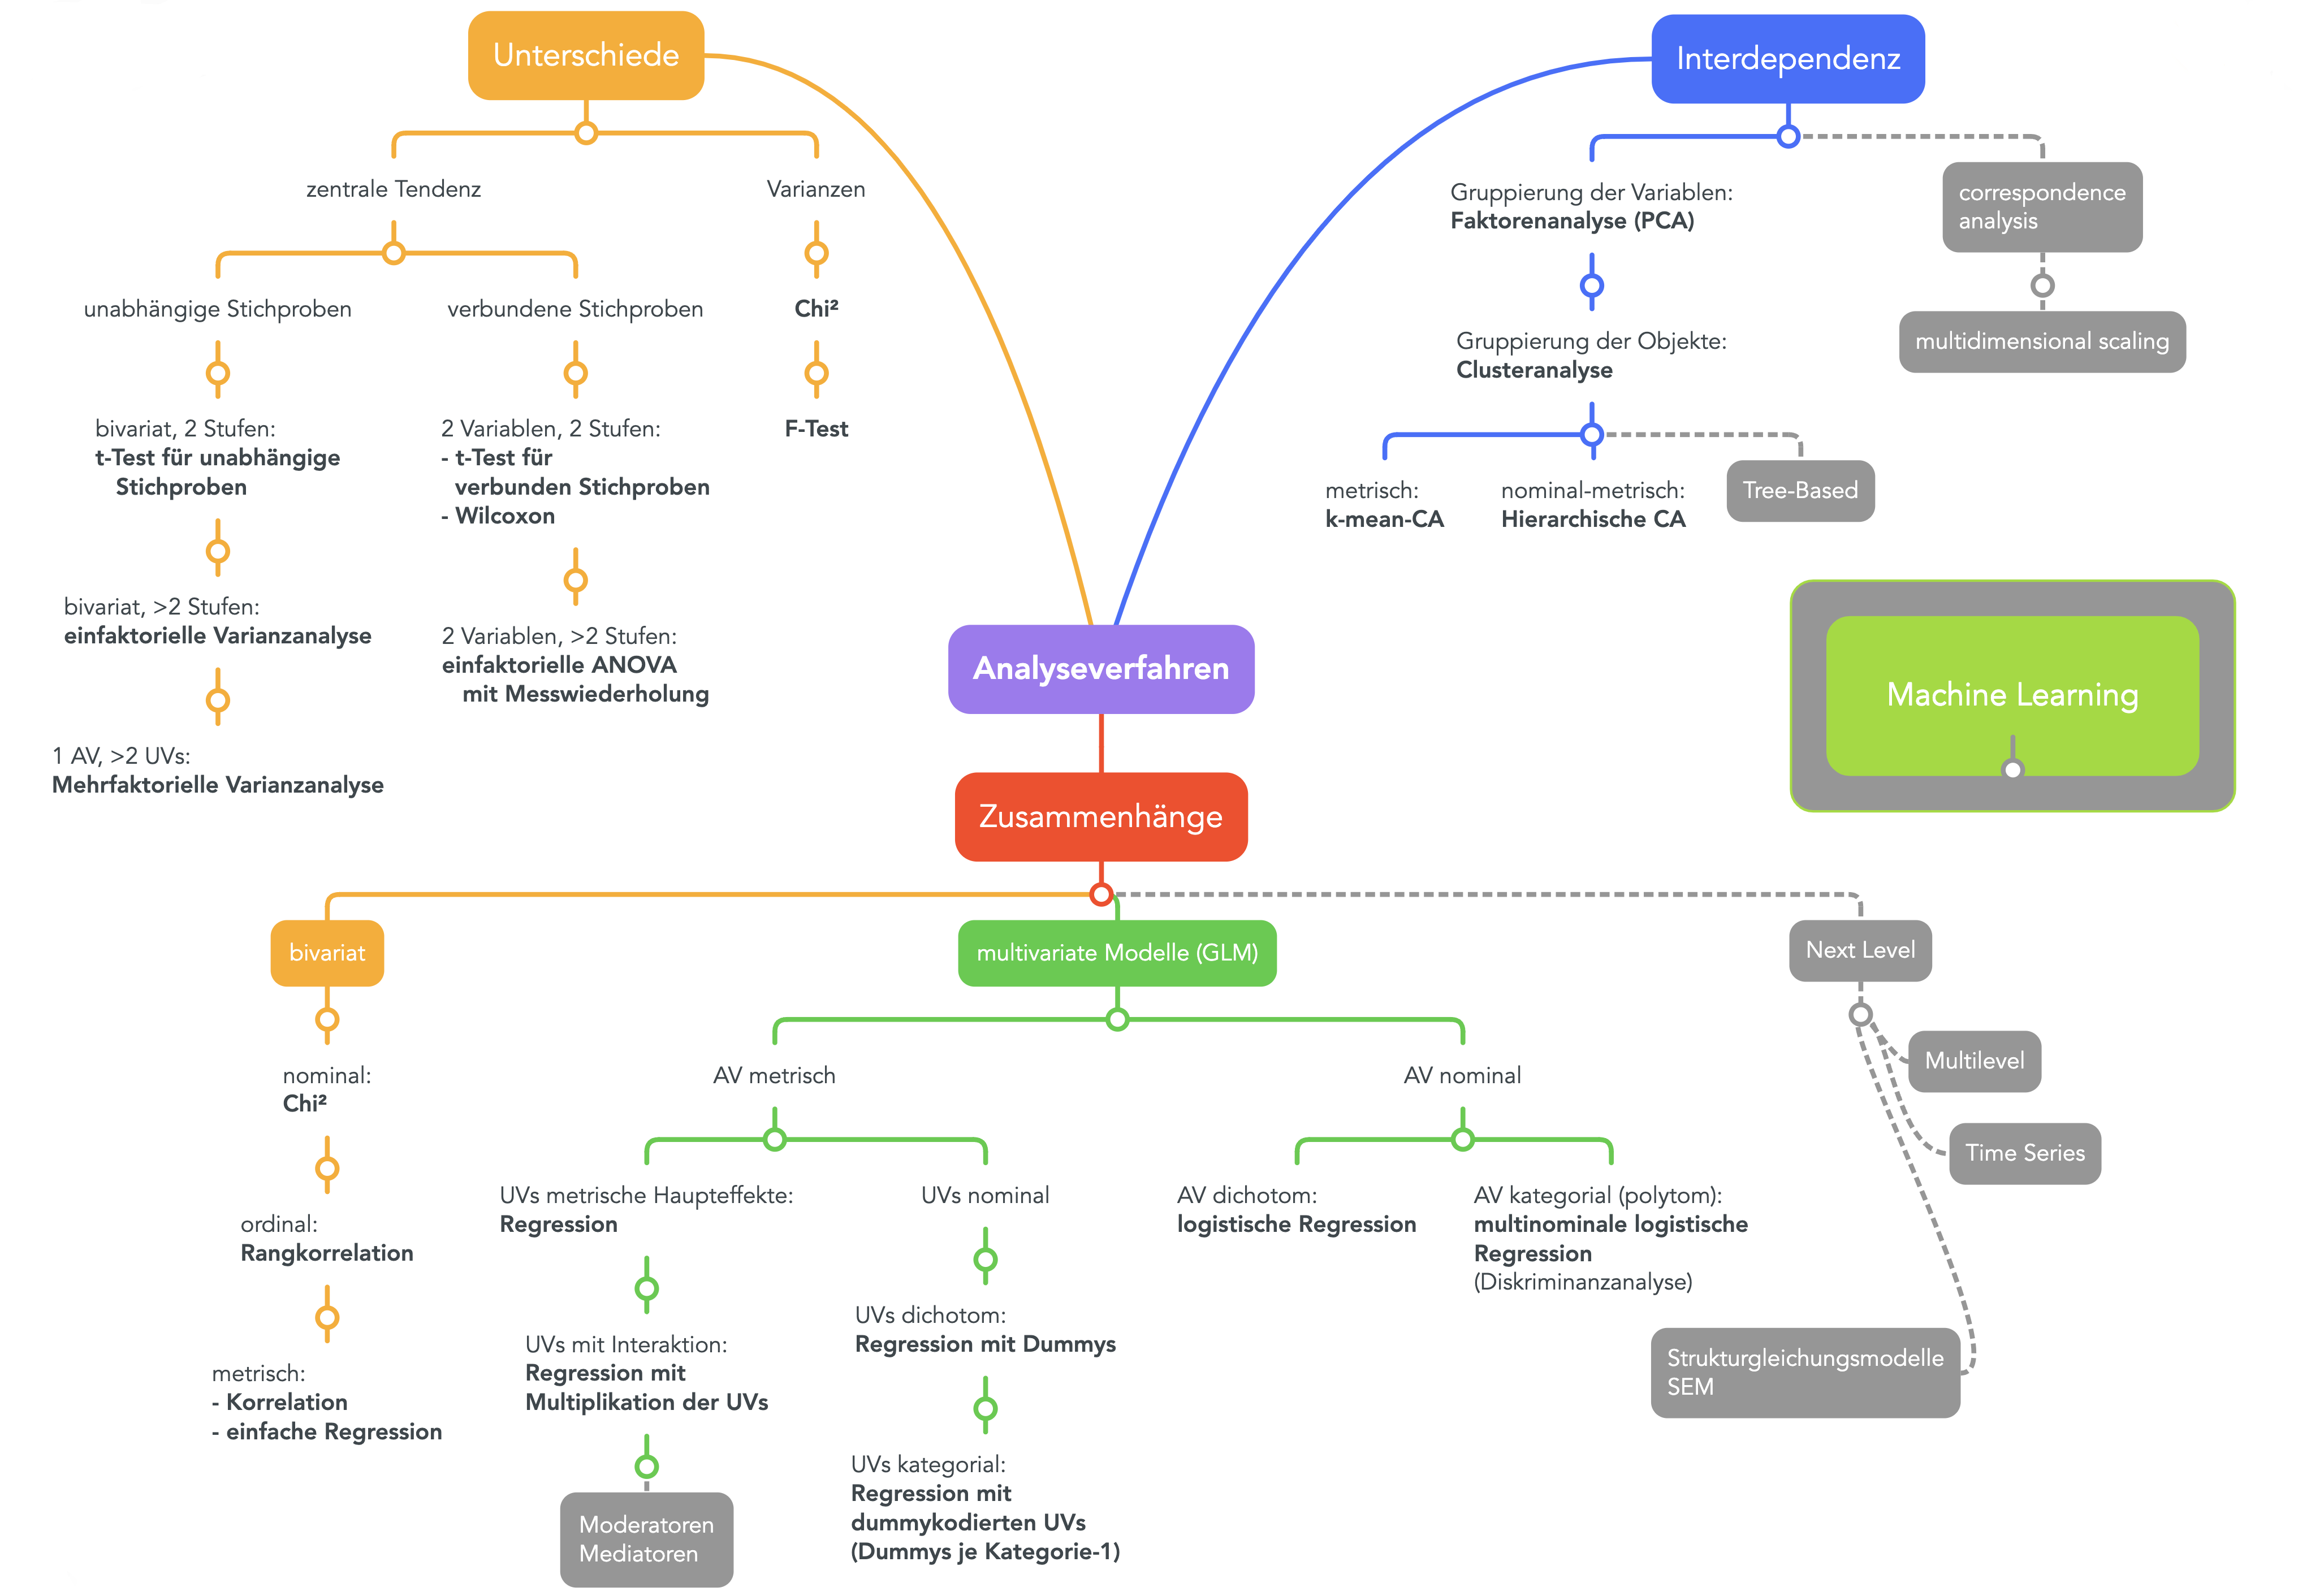
\includegraphics[width=1\textwidth,height=\textheight]{images/Analyseschema-total2.png}

}

\caption{Systematik gesamt}

\end{figure}%

\section*{Zitation dieser Seite}\label{zitation-dieser-seite}
\addcontentsline{toc}{section}{Zitation dieser Seite}

\markright{Zitation dieser Seite}

\begin{center}\rule{0.5\linewidth}{0.5pt}\end{center}

Zitation: Fretwurst, B. (2022). \emph{Statistik und Datenanalyse:
Aufbau. Begleittext zum Modul am IKMZ im HS22.}
https://www.ikmz.uzh.ch/static/methoden/Statistik-Aufbau/. Abrufdatum:
{[}aktuelles Datum{]}.

\begin{center}\rule{0.5\linewidth}{0.5pt}\end{center}

\bookmarksetup{startatroot}

\chapter{Uni- und Bivariate
Statistik}\label{uni--und-bivariate-statistik}

\section{Univariate Statistik}\label{univariate-statistik}

Alle Statistik baut auf Massen zentraler Tendenz und Streumasse auf. Für
das, was wir in diesem Semester tun, brauchen wir eigentlich nur den
Mittelwert (Durchschnitt) und die Standardabweichung. Der Mittelwert
entspricht der Frage: Wo stehen wir im Schnitt? Die Formel gibt an, dass
eine Summe (\(\sum\)) gebildet wird für alle \(x_i\) (von i = 1 bis n)
und diese durch die Anzahl der Fälle n geteilt wird beziehungsweise mit
1/n multipliziert wird:

\begin{align}
 \overline{x} = & \frac{1}{n}\sum_i^n(x_i)
\end{align}

Die Standardabweichung zeigt uns, wie homogen die Fälle in einer
Variable um den Mittelwert streuen. Das ist ein wichtiger Kennwert, weil
derselbe Mittelwert zustande kommt, wenn alle Fälle genau dem Mittelwert
entsprechen (die Standardabweichung wäre 0) oder wenn die Hälfte der
Werte extrem weit links von der Mitte und die andere Hälfte genauso
weit, aber rechts vom Mittelwert liegen (siehe
\textbf{?@fig-homogenitaet}). Die Standardabweichung (s) ist die Wurzel
aus der Varianz (\(s^2\) oder \enquote{V}). Wenn Sie genau hinschauen,
sehen Sie, dass die Varianz im Grunde der Mittelwert der quadrierten
Abweichungen vom Mittelwert ist (vergleichen Sie die Formel mit der
Mittelwertformel, wobei Sie gedanklich
\enquote{\((x_i-\overline{x})^2\)} durch \enquote{\(\overline{x}\)}
ersetzen).

\begin{align}
    s^2 = V = & \frac{1}{n} \sum_i^n(x_i-\overline{x})^2 \\    
    s  = & \sqrt{\frac{1}{n} \sum_i^n(x_i-\overline{x})^2}\\
    \hat{\sigma}^2 = & \frac{1}{n-1} \sum_i^n(x_i-\overline{x})^2\\
    \hat{\sigma} = & \sqrt{\frac{1}{n-1} \sum_i^n(x_i-\overline{x})^2}\\
\end{align}

\begin{tcolorbox}[enhanced jigsaw, coltitle=black, opacitybacktitle=0.6, toptitle=1mm, colbacktitle=quarto-callout-warning-color!10!white, colback=white, toprule=.15mm, opacityback=0, bottomrule=.15mm, arc=.35mm, colframe=quarto-callout-warning-color-frame, leftrule=.75mm, titlerule=0mm, breakable, left=2mm, rightrule=.15mm, title={IYI: Was das \(\frac{1}{n-1}\) bei der Varianz mit Freiheitsgraden zu
tun hat}, bottomtitle=1mm]

Wenn wir die Varianz als durchschnittliche quadrierte Abweichung vom
Mittelwert in der Grundgesamtheit bestimmen wollten und \(\mu\) kennen
würden, ergibt sich folgende Formel für die Varianz: \[ 
\sigma^2 = \frac{1}{n}\sum{(x_i-\mu)^2}
\]

Das Problem ist, dass wir \(\mu\) nicht kennen, wenn wir eine Stichprobe
gezogen haben. Um den unbekannten Parameter (der GG) \(\mu\) schätzen zu
können, ziehen wir den Mittelwert \(\overline{x}\) als
Stichprobenkennwert zur Schätzung von \(\mu\) heran. Dann teilen wir
aber nicht mehr durch n, sondern durch n-1. Das will ich hier erklären.
Die Schätzformel für die Varianz der GG ist (wie oben):

\begin{align}
 \hat{\sigma}^2 = & \frac{1}{n-1} \sum_i^n(x_i-\overline{x})^2
\end{align}

Um deutlich zu machen, dass wir die Varianz der GG nur schätzen, setzen
wir dem \(\hat{\sigma}^2\) ein Dach auf. Die Formel ist schön kurz und
knapp, aber eigentlich sieht man hier nicht gut, was durch das
\(\frac{1}{n-1}\) korrigiert wird. Ein bisschen klarer wird es, wenn wir
deutlich machen, dass es hier einen Korrekturfaktor für die
Stichprobenvarianz gibt, der gekürzt wurde. Eigentlich könnte man ja
schreiben:

\begin{align}
 \hat{\sigma}^2 = & \frac{n}{n-1} \cdot \frac{1}{n}\sum_i^n(x_i-\bar{x})^2\\ 
 \hat{\sigma}^2 = & \frac{n}{n-1} \cdot s^2
\end{align}

Wenn wir den Korrekturfaktor \(\frac{n}{n-1}\) separieren, dann ist der
Rest die einfach Varianz der Stichprobe \(s^2\). Den Korrekturfaktor
bringe ich jetzt mal auf die andere Seite, weil ich damit besser
weitermachen kann. Das tue ich, indem ich durch \(\frac{n}{n-1}\) teile.
Dann stelle ich links noch ein bisschen um.

\begin{align}
 \hat{\sigma}^2 = & \frac{n}{n-1} \cdot s^2 && |\ :\frac{n}{n-1}\\
 \hat{\sigma}^2 \frac{n-1}{n} = & s^2 \\ 
 \hat{\sigma}^2 \frac{n}{n} - \frac{\hat{\sigma}^2}{n} = & s^2 && |\ + \frac{\hat{\sigma}^2}{n}\\
 \hat{\sigma}^2 = & s^2 + \frac{\hat{\sigma}^2}{n} && |\ \sqrt{} \\
 \hat{\sigma} = & s + \frac{\hat{\sigma}}{\sqrt{n}} \\
 \hat{\sigma} = & s + s_{\bar{x}}
\end{align}

Nach ein paar Mal umstellen und dann noch die Waruzel aus allem ziehen,
kommt raus, dass das Sigma der Grundgesamtheit durch die
Standardabweichung in der Stichprobe \(s\) plus dem Standardfehler
\(s_{\bar{x}}\) berechnet wird. Durch die Ableitung wird gezeigt, dass
hinter dem Korrekturfaktor, der an die Stichprobenvarianz angelegt wird
(also \(\frac{1}{n-1}\)) eigentlich steht, dass wir die echte
Standardabweichung \(\sigma\) in der GG um die Standardabweichung der
Mittelwerte (aka Standardfehler) unterschätzen. Der Mittelwert wird je
Stichprobe berechnet und wackelt daher, er hat eben seien Freiheiten. Da
er ein Kennwert ist, der pro gedachter Stichprobe berechnet wird, hat,
nimmmt der Mittelwert der Schätzung der Populationsvarianz \(\sigma^2\)
einen Freiheitsgrad weg, weshalb durch n-1 geteilt wird.

Es gibt Statistiker und Statistikbücher, die sagen, dass auch die
Standardabweichung einer Stichprobe oder einer Grundgesamtheit GG ein
sinnvoller Wert ist (zB, wenn man eine Lehrevaluation in einem Semester
macht und nur etwas über eine Veranstaltung wissen möchte, dann ist das
ja eigentlich eine Vollerhebung der GG der Teilnehmenden.) Diese
Statistiker schreiben \(s^2 = \frac{1}{n}\sum(x_i-\overline{x})^2\).
Andere finden, dass die Standardabweichung eigentlich immer eine
Schätzung für eine Populationsstreuung ist und schreiben daher immer
\(s^2 = \frac{1}{n-1}\sum(x_i-\overline{x})^2\). Wer hat Recht? Is mir
egal. Im Zweifel schreib ich lieber \(\hat{\sigma}^2\), wenn ich
deutlich machen will, dass ein Parameter geschätzt werden soll und
\(s^2\) nur, wenn es um die Stichprobe geht.

\textbf{Im Tutorial schrittweise und graphisch erläutert:}

\url{https://www.youtube.com/embed/jXH1ly3Q87U}

\end{tcolorbox}

:::

\subsection{Z-Transformation}\label{z-transformation}

Die z-Transformation (auch \enquote{Standardisierung}) einer Variable
bedeutet, dass man sie so \enquote{verschiebt}, dass sie um den
Mittelwert 0 streut und zwar mit einer Standardabweichung von 1. Dazu
wird von jedem Wert \(x_i\) der Mittelwert abgezogen und diese Differenz
durch die Standardabweichung geteilt:

\begin{align}    
  z_i= & \frac{x_i-\bar{x}}{s} \label{eq:z-Transformation} 
\end{align}

\subsection{Normalverteilung und
Standardnormalverteilung}\label{normalverteilung-und-standardnormalverteilung}

Mit dem Mittelwert und der Abweichung vom Mittelwert können wir
Verteilungen beschreiben, die sich nach bekannten Gesetzen verteilen:
den Wahrscheinlichkeitsgesetzen. Die Normalverteilung ist dabei die
wichtigste Verteilung. Bei dieser gedachten Idealverteilung steht der
Mittelwert genau in der Mitte und die Streuung ist symmetrisch um den
Mittelwert herum verteilt (wie in Abbildung~\ref{fig-Normalverteilung},
mit dem Mittelwert 2,5 und der Standardabweichung 0,5).

\begin{figure}[H]

\caption{\label{fig-Normalverteilung}Beispiel einer Normalverteilung
(\(\overline{x}\) = 3, s = 0,5)}

\centering{

\includegraphics[width=0.8\textwidth,height=\textheight]{1_Uni_Bivariat_files/figure-pdf/fig-Normalverteilung-1.pdf}

}

\end{figure}%

Wegen dieser Eigenschaften, geben hier also der Mittelwert und die
Standardabweichung die volle Information über die Art der Verteilung ab
\(N(\overline{x},s_x)\). Die Standardnormalverteilung (nach der
z-Transformation) hat einen Mittelwert von 0 und eine Standardabweichung
von 1.

\begin{figure}[H]

\caption{\label{fig-Standardnormalverteilung}Die
Standardnormalverteilung (\(\overline{x}\) = 0, s = 1)}

\centering{

\includegraphics[width=0.8\textwidth,height=\textheight]{1_Uni_Bivariat_files/figure-pdf/fig-Standardnormalverteilung-1.pdf}

}

\end{figure}%

\subsection{Konfidenzintervalle für
Mittelwerte}\label{konfidenzintervalle-fuxfcr-mittelwerte}

Konfidenzintervalle geben einen Wertebereich an, in dem die Parameter
(GG) der Stichprobenkennwerte mit einer angebbaren Wahrscheinlichkeit
liegen.

\begin{align}
   \text{ KI:}& \overline{X}\pm z_1 \cdot SE \label{eq:Konfidenz-Intervall-1}\\
   \text{KI:}& \overline{X}\pm z_1 \cdot \frac{s_x}{\sqrt{n}} \label{eq:Konfidenz-Intervall-2}\\
   \text{KI}_{l.05} =& \overline{x} - 1.96 \cdot \frac{s_x}{\sqrt{n}} \label{eq:Konfidenz-Intervall-3}\\
   \text{KI}_{r.05} =& \overline{x} + 1.96 \cdot \frac{s_x}{\sqrt{n}}\label{eq:Konfidenz-Intervall-4}
\end{align}

\begin{center}\rule{0.5\linewidth}{0.5pt}\end{center}

Mit dieser kleinen Onlineapp können Sie sich mal einen Eindruck davon
verschaffen, wie Konfidenzintervalle reagieren. Schalten Sie sich mal
\enquote{Show Confidence Intervals} und \enquote{Show True Parameter} an
und stellen die \enquote{Number of Experiments} auf 20. Dann suchen Sie
mal, wie viele Konfidenzintervalle den wahren Wert nicht enthalten:

\begin{figure}[H]

{\centering \includegraphics[width=1\textwidth,height=\textheight]{images/KI_interaktiv.jpg}

}

\caption{KI-App}

\end{figure}%

\begin{center}\rule{0.5\linewidth}{0.5pt}\end{center}

\begin{tcolorbox}[enhanced jigsaw, coltitle=black, opacitybacktitle=0.6, toptitle=1mm, colbacktitle=quarto-callout-important-color!10!white, colback=white, toprule=.15mm, opacityback=0, bottomrule=.15mm, arc=.35mm, colframe=quarto-callout-important-color-frame, leftrule=.75mm, titlerule=0mm, breakable, left=2mm, rightrule=.15mm, title={Q\&A: Ist es nicht so, dass das Konfidenzintervall bei grösserer und
genauerer Sicherheit (zb eben 99\% anstatt 95\%) dann kleiner wird? Ich
dachte grosser KI bedeutet kleine Sicherheit und kleines bzw schmales KI
heisst grosse Sicherheit.}, bottomtitle=1mm]

Eine sehr gute Frage, echt! Sie haben richtig erfasst, dass Sicherheit
bei Konfidenzintervallen etwas mit der Wahrscheinlichkeit der
Korrektheit einer Aussage (Sicherheitsniveaus) zu tun hat und
gleichzeitig mit Genauigkeit der Aussage, also der Breite des
Konfidenzintervalls. Diese beiden Konzepte sind aber gegenläufig! Wenn
man in einer Schätzung mehr Sicherheit möchte, geht das nur auf Kosten
der Genauigkeit. Stellen Sie sich vor, sie verabreden sich und sagen,
dass sie es wahrscheinlich zwischen sechs und sieben schaffen. Ihrer
Verabredung ist das aber nicht genau genug und möchte, dass Sie sagen,
wann sie garantiert da sein können. Sie würden dann eher nicht das
Intervall verkleinern und sagen, dass sie es ganz sicher zwischen 18:13
und 18:21 schaffen, sondern das Intervall eher verbreitern und
vielleicht sagen, dass sie es sicher bis 20 Uhr schaffen werden. Wenn
dann verlangt wird, dass sie genauer werden bei höherer Sicherheit
würden Sie vielleicht vorschlagen, dass man sich ein andermal trifft.
Was für ein Stress!

Also, wird eine höhere Sicherheit verlangt (99\%-iges statt 95\%-iges
Signifikanzniveau), wird das Konfidenzintervall breiter.

Sie können das auch gedanklich durchspielen mit der Prognose der
Höchsttemperatur für morgen und was passiert, wenn zum einen gefordert
wird, dass die Prognose sehr genau ist (enges Intervall) und was
passiert, wenn gefordert wird, dass die Prognose mit einer hohen
Garantie auf Richtigkeit versehen wird (Signifikanz- bzw.
Sicherheitsniveau hoch).

\end{tcolorbox}

\section{Bivariate Statistik}\label{bivariate-statistik}

\subsection{Kreuztabellen}\label{kreuztabellen}

Wenn wir Daten analysieren, dann können wir sie visualisieren. Eine sehr
starke Form der Visualisierung sind Tabellen. Der Vorteil von Tabellen
ist, dass sie sehr dicht an den Daten sind, wir also z.B. sehen können
dass, 57 Prozent der Haushalte noch über mindestens ein Radiogerät
verfügen. In der Deutschschweiz (DS) sind es sogar 62 Prozent, während
es in der Romandie (FS) 44 Prozent sind und im Tessin und den weiteren
Teilen der italienischen Schweiz (IS) 63 Prozent. Man kann aus
Kreuztabellen für die beiden berücksichtigten Variablen den
ursprünglichen Datensatz rekonstruieren, weil man weiss wie viele Leute
befragt wurden, wie viel Prozent aus der DS sind, aus der FS und aus der
IS und wie viele Leute jeweils mindestens ein Radio haben. Irgendwann
kann ich Ihnen mal zeigen, wie man aus einer Kreuztabelle eine
Korrelation berechnen kann -- man braucht nicht mehr. Also gut, die
Tabellen enthalten viele Informationen und können, mit ein bisschen
Anleitung, von fast jedem gelesen werden (anders als unserer schönen
Regressions- oder Strukturgleichungsmodelle). Das Problem ist aber, dass
man sehr schnell einschläft, wenn einem so eine Tabelle vorgelesen wird.
Wenn man sie selbst liesst, ist es einfach sehr viel, worauf man schauen
muss, was man vergleichen und dann vielleicht sogar noch texten muss.
Eine Korrelation fast in einem direkt lesbaren Wert das Zusammen, was
Sie vielleicht aus 5*5, also 25 Tabellenzellen mühsam herauslesen und
dann immer noch nur so vom Gefühl her texten können. Tabellen sind also
relativ voraussetzungsfrei interpretierbar, aber es ist sehr ermüdend
und langwierig.

\begin{center}\rule{0.5\linewidth}{0.5pt}\end{center}

\textbf{Beispiel für eine Kreuztabelle mit Link zu mehr (interaktiven)
Kreuztballen:}\\
\includegraphics[width=1\textwidth,height=\textheight]{images/Kreuztabelle.jpg}

\begin{center}\rule{0.5\linewidth}{0.5pt}\end{center}

\subsection{Covarianz und Korrelation}\label{covarianz-und-korrelation}

Vor ein paar Zeilen hatte ich behauptet, man brauche als Kenngrössen in
der Statistik nicht mehr als Mittelwert und Standardabweichung. Das
sollte der Beruhigung dienen und ist ein bisschen gelogen. Ein Merkmal
kann man mit diesen Kenngrössen in der Regel gut beschreiben, aber um
das Zusammenspiel zweier Variablen beschreiben zu können, braucht es
noch eine Kenngrösse: die Kovariation. Wieder etwas vereinfacht und doch
nicht ganz falsch: fast alle multivariate Statistik baut auf
Mittelwerten, Varianzen und Kovarianzen auf.

Kovarianz (cov oder auch C) sieht genauso aus, wie die Definition der
Varianz, nur, dass nicht die Mittelwertabweichungen einer Variablen
quadriert werden, sondern die Mittelwertabweichungen zweier Variablen
multipliziert werden. Berechnet man die Kovarianz einer Variable mit
sich selbst, kommt wieder die Varianz raus. Da Varianz und Mittelwert
nicht standardisiert sind, ist auch die Kovarianz nicht standardisiert.
Rechnet man mit standardisierten Variablen, kommt auch ein
standardisierter Wert für die Kovarianz raus. Da der für Vergleiche von
unvergleichlicher Bedeutung ist, hat auch dieser Kennwert einen eigenen
Namen bekommen: Korrelation (r).

\begin{align}
      cov = C =  & \frac{1}{n}\sum_i^n(x_i-\overline{x})
          (y_i-\overline{y}) \label{eq:Covarianz} \\
      r = &  \frac{\sum_i^n(x_i-\overline{x})
          (y_i-\overline{y})}{n \cdot s_x \cdot s_y} \label{eq:Korrelation}
\end{align}

\begin{center}\rule{0.5\linewidth}{0.5pt}\end{center}

In der folgenden App werden Zusammenhänge illustriert. In dem Beispiel
wurden Studierende gebeten, sich selbst in Bezug auf verschiedene
Eigenschaften auf einer Skala von 0 bis 10 einzuordnen und was sie sich
in Bezug auf dieselbe Eigenschaft von einer:m potentiellen Partner:in
wünschen:\\

Wie man unschwer erkennen kann, hängen diese beiden Variablen
miteinander zusammen -- nicht perfekt (sonst wären alle Punkte auf der
Geraden), aber es ist schon ein deutlicher Zusammenhang. Interessanter
Weise ist der Zusammenhang bei Männern schwächer als bei Frauen. Schauen
Sie doch mal, was Sie dort finden, vergleichen Sie auch mal die
jeweiligen Durchschnittswerte der Selbsteinordnung und dem was sich so
von Partnern gewünscht wird. :-)

\subsection{Bivariate Regression}\label{bivariate-regression}

Die bivariate Regression ist im Grunde eine gehaltvollere Korrelation.
Bei der Regression bestimme ich, im Unterschied zur Korrelation, was die
abhängige Variable sein soll (AV) und was die unabhängige Variable sein
soll (UV). Was die Regression bringt, sieht man in folgenden Formeln.
Wenn wir in der ersten Zeile der Formeln @ref(eq:Mittelwert-Modell)
davon ausgehen, dass wir keine UV haben, die die AV erklärt, dann haben
wir als beste Information nur den Mittelwert. In dem Fall wäre unser
Minimodell also: Die Werte in der Variable \(Y_i\) sind am besten durch
ihren Mittelwert \(\overline{Y}\) \enquote{erklärt}. Übrig bleiben die
Abstände zwischen den gefundenen Werten und diesem Minimodell, also dem
Mittelwert von Y. In der zweiten Zeile @ref(eq:Regressions-gleichung)
sind wir schon klüger und nehmen an, dass eine Variable X dafür
verantwortlich ist, dass die \(Y_i\) so ausfallen, wie sie ausfallen. In
der zweiten Zeile heisst es im Grunde: Die Werte in der AV Y sind
abhängig von der UV X, wobei jeder Wert X mit einem b multipliziert
werden muss und dann ein Rest \(e_i\) bleibt. Damit Y nicht 0 sein muss,
wenn X 0 ist (b*0=0), kommt zu dem \(b_2\) noch ein \(b_1\). Fertig ist
die bivariate Regressionsgleichung.

\begin{align}
  Y_i & = \overline{Y} + e_i  \label{eq:Mittelwert-Modell} \\
  Y_i & = b_1 + b_2X_i + e_i \label{eq:Regressions-gleichung} \\ 
  \hat{Y_i} & = b_1 + b_2X_i \label{eq:Regressions-Modell} \\
  Y_i & = \hat{Y_i}+e_i \label{eq:Varianz-Modell-Residuum}
\end{align}

Jetzt könnten wir noch die vorhergesagten \(\hat{Y}\) (gekennzeichnet
durch ein Dach) durch das Modell abbilden, wobei dann einfach kein
\(e_i\) bleibt (dritte Zeile @ref(eq:Regressions-Modell)). In der
untersten Formel @ref(eq:Varianz-Modell-Residuum) haben wir die in der
Stichprobe gemessenen \(Y_i\), die gleich gesetzt sind mit den
geschätzten \(Y_i\) und dem Rest \(e_i\).

Das \(b_2\) gibt jetzt an, um wie viel Y grösser (oder kleiner) ist,
wenn X um eine Einheit seiner Skala grösser wird. Die b's sind also
skalenabhängig. Weil das nicht immer leicht zu interpretieren ist und
uns oft die Skalierung nicht weiter interessiert, wurden die
standardisierten Regressionkoeffizienten erfunden. Bei diesen steht im
Grunde wieder eine z-Transformation im Hintergrund, die die Skala
\enquote{herausrechnet}, indem durch die Standardabweichung geteilt
wird.

Die standardisierten Regressionskoffizienten geben einen Zusammenhang in
Standardabweichungen an: Wenn x um eine Standardabweichung grösser ist,
um wie viele Standardabweichungen ist dann y grösser (kann negativ
sein)?

Sie sind definiert als: \(BETA = b\cdot\frac{s_x}{s_y}\)

Die BETAs\footnote{Es ist recht ungünstig, dass die standardisierten
  Regressionskoeffizienten (fast) genauso heissen wie die Parameter
  \(\beta\) der b's. Ich versuche das verbal deutlich zu machen, indem
  ich \enquote{beeta} mit langem ee sage, wenn ich die standardisierten
  Regressionkoeffizienten BETA meine und \enquote{betta} sage (mit sehr
  kurzem e), wenn ich die griechischen \(\beta\) meine. Wenn Sie
  irgendwo ausserhalb eines Statistiklehrbuchs BETA lesen oder (sogar
  immer häufiger) \(\beta\), dann verlassen Sie sich darauf, dass immer
  die standardisierten Regressionskoeffizienten gemeint sind und nie die
  Parameter der Regressionskoeffizienten in der Grundgesamtheit, weil
  wir die nie kennen werden und deshalb in empirisch wissenschaftlichen
  Publikationen so gut wie nie die Rede von unbekannten Parametern sein
  wird, sondern immer von den Kennwerten der Stichprobe, also den
  standardisierten Regressionskoeffizienten BETA. Didaktisch ist das
  blöd, aber es ist so und wenn ich jetzt was ganz Neues erfinde, dann
  bringt Ihnen das auch garnix.)} sind den partiellen Korrelationen sehr
ähnlich: +1 ist ein perfekter positiver Zusammenhang, 0 kein
Zusammenhang und -1 ein perfekter negativer Zusammenhang. Interpretieren
würde ich ab 0.1, wenn sie signifikant sind.

\section{Inferenzstatistik}\label{inferenzstatistik}

Was in den Daten ist, die wir analysieren, das ist in den Daten --
Punkt. Wir können Daten mit all diesen Tools untersuchen. Dafür brauchen
wir natürlich vollständige Daten über das, was wir untersuchen wollen.
Die haben wir aber oft nicht, weil es schlicht zu teuer ist und alle
Menschen unfassbar nerven würde, wenn alle Sozialforscher:innen und
Psycholog:innen und Wirtschaftswissenschaftler:innen usw. dauernd alle
Menschen befragen würden. Das machen wir nicht, weil eine faszinierende
Eigenschaft der Statistik ist, dass wir aus Teildaten Schlüsse auf die
\enquote{Gesamt-Daten} ziehen können. Dieses Schliessen nennt man
Inferenz (besser über das Englische zu merken: to infer). Dafür ist es
notwendig, dass wir die Daten ohne bewussten Bias aus den Gesamtdaten
entnommen haben.

Einen Bias ausschliessen können wir, wenn wir den Zufall walten lassen.
Zufall ist nichts anderes als das
Nicht-bewusst-oder-unbewusst-Auswählen. Wenn wir zufällig gezogen haben,
dann haben wir eine gute Chance auf ein unverzerrtes Abbild der
Grundgesamtheit, die uns interessiert. Dann berechnen wir die ganzen
Kennwerte der deskriptiven Statistik für die Stichprobe und können
anhand der Zufallsgesetze bzw. Wahrscheinlichkeitstheorie auf die
Verteilung in der Grundgesamtheit schliessen. Dabei bleibt eine
Unsicherheit, weil der Zufall zufällig ungünstig ausfallen kann (wir
haben auch schon Pferde kotzen sehen).

Wir können allerdings sagen, wie wahrscheinlich bzw. unwahrscheinlich es
ist, dass wir extrem viel Pech hatten mit unserer Stichprobenziehung.
Dabei sind wir sehr vorsichtig und schätzen und testen konservativ. Die
Frage ist also immer: Kann ich, wenn ich ganz vorsichtig und konservativ
bin, ausschliessen, dass ich sehr viel Pech bei der Ziehung meiner
Zufallsstichprobe hatte? Das Pech bei der Zufallsziehung wird als
Nullhpyothese bezeichnet (H0). Die sagt nämlich, wir haben eigentlich
keinen Unterschied oder Zusammenhang und trotzdem in unserer Stichprobe
den Unterschied (abweichend von 0) gefunden, den wir gefunden haben.
Wenn wir -- bei aller Vorsicht -- sagen, dass ein Effekt (Unterschied
oder Zusammenhang) so gross ist, dass die Nullhypothese so
unwahrscheinlich wird (5\% Irrtumswahrscheinlichkeit), dass wir sie
ablehnen können, dann haben wir etwas gefunden, etwas Signifikantes!

Ob das signifikante Ergebnis unserer Theorie entspricht oder nicht, das
müssen wir dann noch schauen, aber erstmal können wir festhalten, dass
wir überhaupt etwas gefunden haben und nicht sagen müssen: Wir haben
zwar einen positiven Zusammenhang gefunden, aber statistisch müssen wir
die Nullhypothese beibehalten, dass der Zusammenhang positiv sein
könnte, aber auch 0 oder negativ. Wenn wir nichts ausschliessen können,
wissen wir nichts. Die H0 bedeutet also, dass wir statistisch nichts
feststellen können und daher auch nicht zu Wissen gelangen. Wenn Sie
irgendwo lesen, dass jemandem in seinen Analysen eine H0 zugute kommt
oder die Annahme einer Nullhypothese als Erkenntnis gefeiert wird, seien
Sie sehr skeptisch! Meistens liegt ein Denkfehler zugrunde: Dass ich 0
nicht ausschliessen kann, heisst nicht, dass ein Zusammenhang oder
Unterschied nicht existiert. Wenn wir z.B. in einer Stichprobe einen
Unterschied zwischen zwei Gruppen gefunden haben, dann ist die
Wahrscheinlichkeit dafür, dass der Unterschied in der Grundgesamtheit 0
ist genauso gross, wie die Wahrscheinlichkeit, dass der Unterschied in
der Grundgesamtheit doppelt so gross ist, wie der den wir gefunden
haben. Das liegt daran, dass die Glockenkurve der Fehlerverteilung um
einen gefundenen Wert symmetrisch um den gefunden Unterschied verteilt
ist.

\begin{center}\rule{0.5\linewidth}{0.5pt}\end{center}

\textbf{Mit dieser App lässt sich etwas mit der Normalverteilung
experimentieren:}\\
\includegraphics[width=1\textwidth,height=\textheight]{images/shiny-Normalverteilung.jpg}

\begin{center}\rule{0.5\linewidth}{0.5pt}\end{center}

\subsection{Hypothesentesten}\label{hypothesentesten}

Erkenntnistheoretisch prüfen wir unsere Hypothesen, um unser Wissen
immer weiter abzusichern, bzw. Veränderungen festzustellen. Eine Theorie
muss sich in der empirischen Sozialforschung immer wieder an neuen Daten
bewähren. Wiedersprechen meine Daten immer wieder (replizierbar) der
Theorie, wird sie modifiziert oder aufgegeben, wenn wir was Besseres
haben.

Bei der statistischen Analyse gibt es neben unseren wissenschaftlichen
Hypothesen auch rein statistische Fragen. Wenn wir einen Mittelwert in
unserer Stichprobe finden, ist der sicher nicht identisch mit dem
entsprechenden Parameter \(\mu\) in der Grundgesamtheit (Population). Es
stellt sich also immer die Frage nach möglichen Unschärfen. Über die
statistischen Hypthesen können wir Aussagen treffen, wenn wir den
Gesetzen der Wahrscheinlichkeit (Stochastik) eine Chance geben, also
wenn wir Zufallsstichproben ziehen. Diese Zufallsstichproben ziehen wir
aber nicht aus der Grundgesamtheit, also allen Objekten oder Subjekten,
für die unsere Theorie Gültigkeit beansprucht. Wir ziehen Stichproben in
einem abgesteckten Zeitrahmen und unter den Bedingungen der Machbarkeit.
Wer kein Telefon hat, wird nicht angerufen. Um dieser Unterscheidung
nachdruck zu verleihen, unterscheide ich Grundgesamtheit und
Auswahlgesamtheit. Für letztere gilt: Jedes Element der
Auswahlgesamtheit hat eine von 0 verschiedene Chance in die Stichprobe
zu gelangen.

\begin{enumerate}
\def\labelenumi{\arabic{enumi}.}
\tightlist
\item
  Könnte in der Auswahlgesamtheit der wahre Wert auch 0 sein, oder ein
  anderes Vorzeichen haben?
\item
  Die Nullhypothese ist eine statistische Hypothese gegen
  Falschentscheidungen aufgrund von Zufallsziehungen.
\item
  Nullhypothesen werden anhand von bekannten Verteilungen getestet.
\end{enumerate}

\begin{figure}

\centering{

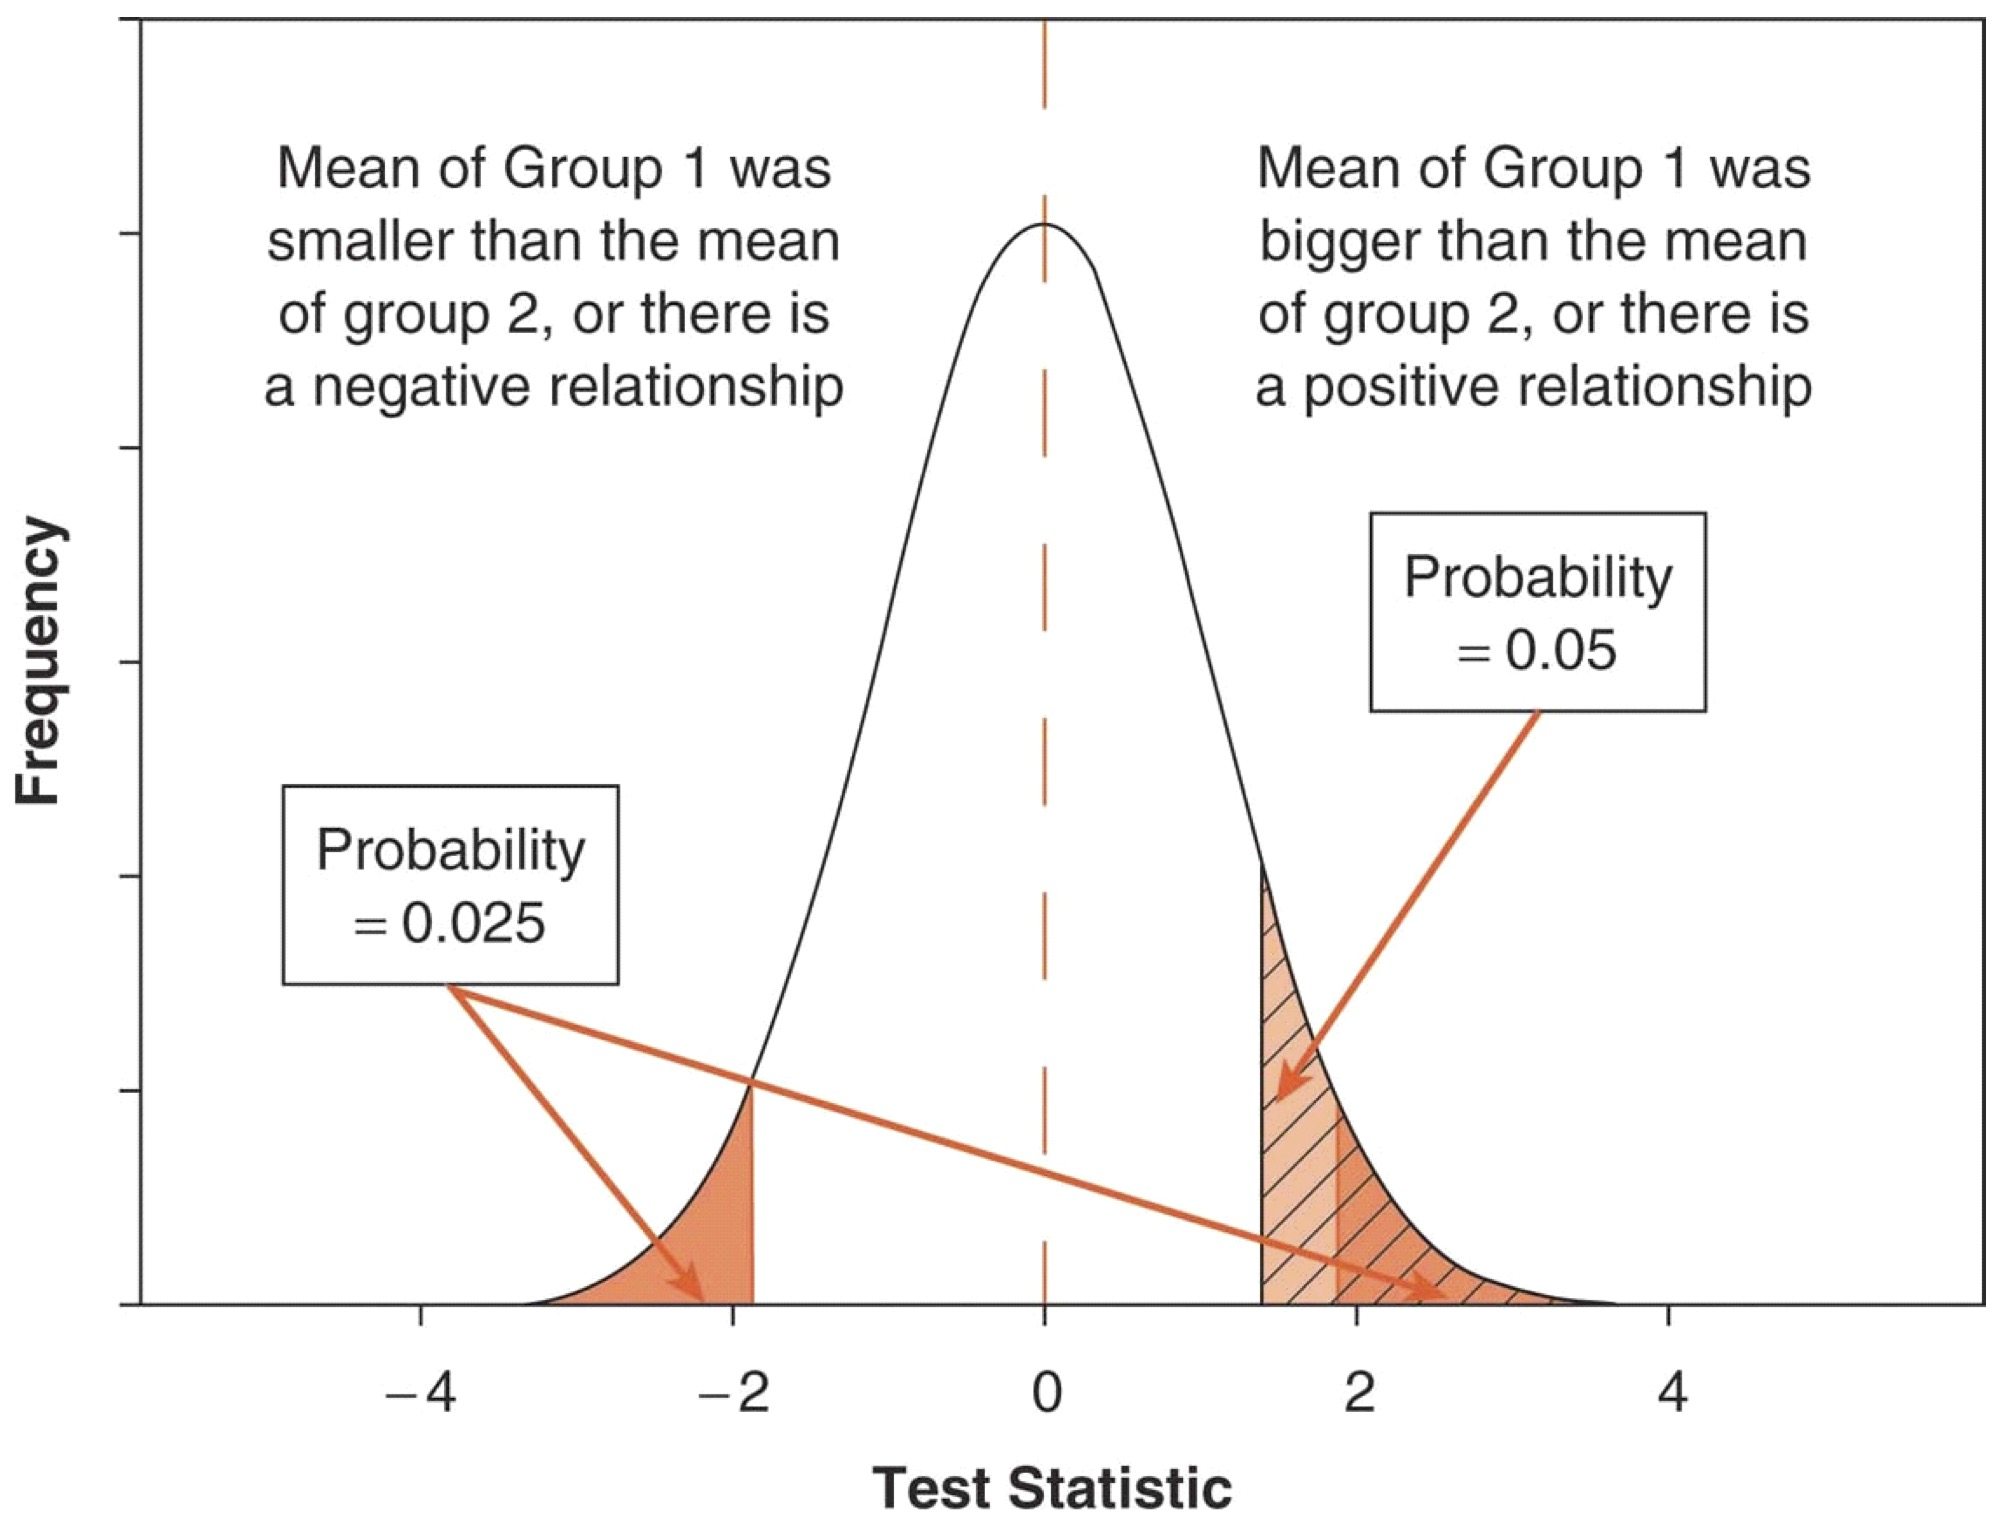
\includegraphics[width=0.8\textwidth,height=\textheight]{images/TestStat1.jpg}

}

\caption{\label{fig-Hypothesen}Hypothesentesten}

\end{figure}%

\begin{center}\rule{0.5\linewidth}{0.5pt}\end{center}

\textbf{Link zu einer guten App zum Probieren:}\\
\href{https://antoinesoetewey.shinyapps.io/statistics-201/}{\includegraphics{images/Hypothesen-testen.jpg}}
------------------------------------------------------------------------

\bookmarksetup{startatroot}

\chapter{GLM -- Regression}\label{glm-regression}

\section{Das lineare Modell (GLM)}\label{das-lineare-modell-glm}

\subsection{Die Idee vom Modell}\label{die-idee-vom-modell}

Für das Ergebnis der Datenerhebung wird ein Modell entworfen, das
Zusammenhänge einfach darstellt. Da das Modell nie zu 100\% das Ergebnis
treffen wird, bleibt ein Rest, den wir Modellfehler oder einfach Fehler
nennen.

\begin{tcolorbox}[enhanced jigsaw, coltitle=black, opacitybacktitle=0.6, toptitle=1mm, colbacktitle=quarto-callout-note-color!10!white, colback=white, toprule=.15mm, opacityback=0, bottomrule=.15mm, arc=.35mm, colframe=quarto-callout-note-color-frame, leftrule=.75mm, titlerule=0mm, breakable, left=2mm, rightrule=.15mm, title={Grundmodell}, bottomtitle=1mm]

Ergebnis = (Modell) + Fehler

Zum Beispiel ist der Mittelwert das einfachste univariate «Modell» einer
Variablen, wobei \(\overline{x}\) das Modell ist und die Abweichungen
von \(x_i\) sind die Fehler: \(x_i = \overline{x} + Fehler_i\).

\end{tcolorbox}

Das lineare Modell ist die Basis von fast allem. Auch was Sie schon
kennen, wird unter dem Konzept \enquote{lineares Modell}
zusammengefasst:

\begin{itemize}
\tightlist
\item
  Varianzanalyse
\item
  (Korrelation ist auch linear, aber eigentlich kein Modell)
\item
  Regression
\end{itemize}

Das lineare Modell ist auch nicht auf lineare Zusammenhänge beschränkt.
Es kann sehr gut mit kurvilinearen Zusammenhängen umgehen. Also, wenn
zum Beispiel bei einer Gesamtnachrichtenlage mit sehr hohem
Nachrichtenwert der Umfang des Medienkonsums steigt. Irgendwann erfährt
diese Wirkung einen Deckeneffekt, weil niemand auf Dauer 24h am Tag
Medien konsumieren kann. Vielleicht steigt der Nachrichtenkonsum mit dem
Nachrichtenwert sogar Anfangs exponentiell (wie Coronazahlen) und hat
dann bald einen Umkehrpunkt und strebt gegen ein mögliches Maximum.
Selbst solche komplexeren Zusammenhänge können in einem linearen Modell
dargestellt werden.

Die höhere Statistik wie Strukturgleichungsmodelle, Zeitreihenanalysen
(Forcastings oder Laten-Growth-Curve-Modelle) bauen alle auf dem
linearen Modell auf. Und auch Computational Science nutzt Modelle und
zwar überwiegend als Basis die linearen Modelle.

\section{Regression Einführung}\label{regression-einfuxfchrung}

Die Regression ist das einfachste und gleichzeitig mächtigste Werkzeug
multivariater Datenanalyse. Aus den Kovarianzen mehrerer Variablen wird
eine Funktion mit wenigen Kennwerten berechnet. Diese Kennwerte geben
Auskunft darüber, wie etwas, das wir erklären wollen mit Dingen
zusammenhängt, von denen wir glauben (hypothetisch annehmen), dass Sie
Erklärungen liefern können. Man muss also vorher sagen, was man erklären
will und womit man es erklären will. Die zu erklärende Grösse nennt man
in der Sozialwissenschaft (und anderen Disziplinen): abhängige Variable
(AV oder DV) und die Erklärungsgrössen nennt man: unabhängige Variablen
(UV oder IV).

Die Regression baut auf Kovarianzen auf (bzw. Korrelationen, die wir uns
besser vorstellen können). Die Regressionsgerade wird bei einer
bivariaten Regression durch eine Konstante (in der Abbildung
Abbildung~\ref{fig-KorrelationRegression} ist sie 1) und einem Anstieg
je Variable gekennzeichnet (in der Abbildung ist es 0,5 für die eine UV
= x).

\begin{figure}

\centering{

\captionsetup{labelsep=none}\includegraphics[width=0.8\textwidth,height=\textheight]{images/Korrelation_Regression.jpg}

}

\caption{\label{fig-KorrelationRegression}}

\end{figure}%

\subsection{Notation der (multivariaten)
Regression}\label{notation-der-multivariaten-regression}

Auch wenn es sinnvoll war, bei der bivariaten Regression die Konstante
«a» zu nennen, soll ab jetzt die Bezeichnung der
Regressionskoeffizienten etwas geändert werden:

\begin{tcolorbox}[enhanced jigsaw, coltitle=black, opacitybacktitle=0.6, toptitle=1mm, colbacktitle=quarto-callout-note-color!10!white, colback=white, toprule=.15mm, opacityback=0, bottomrule=.15mm, arc=.35mm, colframe=quarto-callout-note-color-frame, leftrule=.75mm, titlerule=0mm, breakable, left=2mm, rightrule=.15mm, title={Wir ändern die Notation etwas:}, bottomtitle=1mm]

\[
\begin{aligned}
 Y & = a + bX + e \\ 
 ➪ & = b_1 + b_2X_2 + e  
\end{aligned}
\]

\end{tcolorbox}

\includegraphics[width=1\textwidth,height=\textheight]{images/APA_Regression.jpeg}

\begin{tcolorbox}[enhanced jigsaw, coltitle=black, opacitybacktitle=0.6, toptitle=1mm, colbacktitle=quarto-callout-note-color!10!white, colback=white, toprule=.15mm, opacityback=0, bottomrule=.15mm, arc=.35mm, colframe=quarto-callout-note-color-frame, leftrule=.75mm, titlerule=0mm, breakable, left=2mm, rightrule=.15mm, title={Warum die Schreibweise ändern?}, bottomtitle=1mm]

\begin{itemize}
\tightlist
\item
  In Tabellen (auch in R) steht die Konstante (a) in der Spalte der b's
  (estimates).
\item
  Und weil wir im Multivariaten mehrere X und zugehörige b's haben,
  nummerieren wir sie durch, wobei wir in der ersten Zeile mit \(b_1\)
  für die Konstante anfangen.
\item
  Uuuuuund: In der Matrixschreibweise würde man B als Vector für die
  Regressionskoeffizienten nehmen, wobei die Konstante in der ersten
  Zeile steht.
\end{itemize}

\end{tcolorbox}

Das bedeutet, dass bei einer bivariaten Regression zwei b's die Lage der
Regressionsgeraden bestimmen: Das ist zum einen die Konstante \(b_1\)
und zum anderen der Anstieg \(b_2\) für die Gerade. In der
Abbildung~\ref{fig-RegressionsGeraden}\vpageref{fig-RegressionsGeraden}
sehen Sie links zwei Regressionsgeraden mit unterschiedlichen \(b_2\)
(rot positiv und grün negativ). Auf der rechten Seite sehen Sie drei
Regressionsgeraden mit unterschiedlichen \(b_1\), wobei das b der roten
Gerade am grössten ist (knapp 70), grün am kleinsten (bischen über 20)
und blau in der Mitte liegt (knapp 40).

\begin{figure}

\centering{

\includegraphics[width=0.8\textwidth,height=\textheight]{images/Regressionsgeraden.jpg}

}

\caption{\label{fig-RegressionsGeraden}b's bei bivariaten Regressionen}

\end{figure}%

\begin{center}\rule{0.5\linewidth}{0.5pt}\end{center}

\begin{center}\rule{0.5\linewidth}{0.5pt}\end{center}

\section{Das Modell und die Regressionsgleichung als
Schätzung}\label{das-modell-und-die-regressionsgleichung-als-schuxe4tzung}

Die formelle Schreibweise eines Regressionsmodells enthält griechische
Buchstaben um zu signalisieren, dass es sich hier um unbekannte Grössen,
die Parameter in der Grundgesamtheit, handelt. So lange wir über die
Qualität und die Eigenschaften von Regressionsrechnungen sprechen, wird
uns der Unterschied zwischen \(\beta\)'s und b's interessieren.

Als Gleichung heisst das, dass die Abhängige Variable \(Y_i\) durch eine
gewichtete Summe (siehe Formel Gleichung~\ref{eq-RegressionParameter})
von einer oder mehreren unabhängigen Variablen erklärt wird. Diese UVs
werden in der Regel mit X gekennzeichnet und weil es mehrere davon geben
kann, werden sie durchnummeriert. Also mit dem Subscript i für das
Durchzählen werden sie griechisch für die Parameter als
\(\beta_2X_{i2}\) bezeichnet oder eben als \(\beta_3X_{i3}\) usw. Dann
gibt es noch den Rest \(U_i\). Das ist also das theoretische
statistische Modell, dessen \textbf{Parameter} wir mit
\textbf{Kennwerten} schätzen wollen.

\begin{equation}\phantomsection\label{eq-RegressionParameter}{
   Y_i = \beta_1 + \beta_2X_{i2} + \beta_3X_{i3} + U_i
}\end{equation}

Wenn man mal genau schaut was nach der Stichprobenziehung eigentlich
noch variabel ist, dann wird klar, dass die \(Y_i\) in der Datenerhebung
gemessen wurden und damit Werte enthalten, die wir nicht mehr ändern.
Das Gleiche gilt für die \(X_i\)-Werte der Variablen \(X_2\) und
\(X_3\). Also sind diese Grössen eigentlich keine \enquote{Variablen}
mehr, sondern längst durch echte Werte \enquote{fixiert}. Zu schätzen
sind nur die b's, also \(b_1\), \(b_2\) und \(b_3\) (wie in
Gleichung~\ref{eq-RegressionsKennwerte}). Wenn wir die
Regressionskoeffizienten, die b's in unserer Stichprobe, berechnet
haben, müssen wir uns noch fragen, wie gut, also unverzerrt und genau
sie die unbekannten Parameter (\(\beta\)S) messen, also -- etwas
technischer ausgedrückt -- ob die b die \(\beta\) erwartungstreu und
effizient schätzen. Dafür gibt es einige Voraussetzungen, die wir uns
später {[}in Kapitel noch nicht da{]} noch anschauen werden. Am Ende der
Formel steht das \(e_i\) für die Fehler, also den unerklärten Rest der
Varianz, der zwischen den durch das Modell geschätzten Werten
(gekennzeichnet mit einem Dach als \(\hat{Y_i}\)) und den gemessenen
Werten liegt. Während die s's die Schätzer für die \(\beta\)s sind, ist
das \(e_i\) kein Schätzer für \(U_i\). Das liegt daran, dass das \(e_i\)
nur eine Fehlerstreuung in der Stichprobe ist und \(U_i\) viel mehr
angibt, dass unberücksichtigte Einflussgrössen und ein stochastischer
Rest nicht vom Modell abgebildet sind.

\begin{equation}\phantomsection\label{eq-RegressionsKennwerte}{
 Y_i  = b_1 + b_2X_{i2} + b_3X_{i3}+e_i
}\end{equation}

Bei einer Regression mit zwei UVs wird praktisch eine Ebene in die
Punktwolke gelegt (siehe Abbildung~\ref{fig-Regressionsebene}). Wir
schätzen aber eine multivariate Regression, damit wir bivariat
interpretieren können, also je UV sagen, wie stark der Effekt auf die AV
ist. Insofern interpretieren wir je Variable nur ein b, was dem Ansteig
(Zusammenhang) einer UV mit der AV entspricht. Das können wir machen,
weil die Statistik beziehungsweise unser Statistikprogramm die
\enquote{Kontrolle} der übrigen Variablen übernimmt und wir schön die
kontrollierte bivariate Beziehung interpretieren können. Die b's
beschreiben dabei die Gerade, die die Ebene an der Stelle bildet, die
für die andere Variable der Durchschnitt ist. Bei drei UVs spannen die
b's zusammen eigentlich einen Raum auf, was sich aber niemand mehr
visuell vorstellen kann. Die Statistik kann das aber und erledigt das so
für uns, dass wir uns immer nur die Beziehungen anhand der jeweiligen
b's der einzelnen UV's anschauen können.

\begin{figure}

\centering{

\includegraphics[width=0.75\textwidth,height=\textheight]{images/IV_Regression.png}

}

\caption{\label{fig-Regressionsebene}Regressionsebene bei zwei UVs}

\end{figure}%

\begin{center}\rule{0.5\linewidth}{0.5pt}\end{center}

Hier wird eine Regression recht gut als Punktwolke visualisiert:
\url{http://shiny.calpoly.sh/3d_regression/}.

\begin{figure}[H]

{\centering \includegraphics[width=1\textwidth,height=\textheight]{images/Regression-bivariat.jpg}

}

\caption{Regression}

\end{figure}%

\begin{center}\rule{0.5\linewidth}{0.5pt}\end{center}

\begin{center}\rule{0.5\linewidth}{0.5pt}\end{center}

\textbf{Zwischenaufgabe: Schreiben Sie die Formel für die einfache
bivariate Regression auf?}

Lösung anschauen

\[
  Y_i = b_1 + b_2X_{i2} + e_i 
\]

\begin{center}\rule{0.5\linewidth}{0.5pt}\end{center}

\begin{tcolorbox}[enhanced jigsaw, coltitle=black, opacitybacktitle=0.6, toptitle=1mm, colbacktitle=quarto-callout-important-color!10!white, colback=white, toprule=.15mm, opacityback=0, bottomrule=.15mm, arc=.35mm, colframe=quarto-callout-important-color-frame, leftrule=.75mm, titlerule=0mm, breakable, left=2mm, rightrule=.15mm, title={Q\&A: Wann genau bezeichnet man Kennwerte wie den Mittelwert, die
Varianz oder die Standardabweichung als unbekannte Parameter? Also wann
benutzt man die Symbole \(\mu\), \(\sigma^2\) oder \(\sigma\) und was
ändert das im Vergleich zu den Bezeichnung wie s und \(s^2\)?}, bottomtitle=1mm]

\(\mu\), \(\sigma^2\) oder \(\sigma\) sind Parameter der
Grundgesamtheit. Das sind \enquote{Kennwerte} der Grundgesamtheit, die
wir in der Realität allerdings eigentlich nie kennen. Deshalb wollen wir
aus den Kennwerten einer Stichprobe (z.B. Mittelwert: \(\overline{x}\),
Varianz: \(s^2\) etc.) auf die korrespondierenden Parameter der
Grundgesamtheit (Mittelwert: \(\mu\), Varianz \(\sigma^2\) etc.)
schliessen.

\begin{itemize}
\tightlist
\item
  Der Mittelwert einer Stichprobe wird mit \(\overline{x}\), die Varianz
  mit \(s^2\) bezeichnet.\\
\item
  Der Mittelwert in der Grundgesamtheit wird mit \(\mu\), die Varianz
  mit \(\sigma^2\) bezeichnet
\end{itemize}

\end{tcolorbox}

\section{Die Regressionskoeffizienten
b}\label{die-regressionskoeffizienten-b}

\subsection{Im bivariaten Modell}\label{im-bivariaten-modell}

Das b ist im bivariaten Modell:
\(b = \frac{\sum{(X- \overline{X})(Y- \overline{Y})}}{\sum{(X- \overline{X})^2}}\).
Wenn Sie genau hinsehen, erkennen Sie über dem Bruch den oberen Teil der
Kovarianz \(\sum{(X- \overline{X})(Y- \overline{Y})}\) und im unteren
Teil der Varianz von X (ohne dass jeweils durch n geteilt wird). Nachem
man das ein bisschen umgestellt hat, erhält man
\(r_{YX}\cdot \frac{s_y}{s_X}\) und wenn man durch \(\frac{s_y}{s_X}\)
geteilt hat, steht da, dass \(r_{YX} = b \cdot \frac{s_X}{s_Y}\) ist. Im
Grunde ist die Korrelation also ein standardisiertes b.

\begin{tcolorbox}[enhanced jigsaw, bottomrule=.15mm, arc=.35mm, colframe=quarto-callout-note-color-frame, leftrule=.75mm, rightrule=.15mm, breakable, left=2mm, colback=white, toprule=.15mm, opacityback=0]

\vspace{-3mm}\textbf{Regressionskoeffizient b (aka Steigungskoeffizient) und r}\vspace{3mm}

\begin{align}
  b & = \frac{\sum{(X- \overline{X})(Y- \overline{Y})}}{\sum{(X- \overline{X})^2}} \\
 {} & = \text{... Then A Miracle Occurs ...}  \\
 {} & =r_{YX}\cdot \frac{s_y}{s_X} \\
 r_{YX} & = b \cdot \frac{s_X}{s_Y}
\end{align}

\includegraphics{images/MirracleOccurse.jpeg}

\end{tcolorbox}

\subsection{Bei zwei UVs und zwei b's}\label{bei-zwei-uvs-und-zwei-bs}

Wenn wir mit Hilfe der Ordenary-Least-Squares-Methode (OLS) eine Formel
für die b's bestimmt haben, kommt folgende Formel
Gleichung~\ref{eq-FormelFuerBs} für das \(b_2\) der Variable
\(X_2\)\footnote{In den tiefergestellten Subscripten steht bei den r's
  immer nur 2. Das heisst \(r_{Y2}\) kennzeichnet die Korrelation
  zwischen \(Y\) und \(X_2\).} heraus:

\begin{equation}\phantomsection\label{eq-FormelFuerBs}{
\begin{aligned}
 b_2 & = \frac{r_{y2}-r_{23}r_{y3}}{(1-R_{2.3}^2)}\frac{s_y}{s_2}
\end{aligned}
}\end{equation}

Die Formel hat es in sich. Aber schauen Sie sich die Formel mal ganz in
Ruhe und stückchenweise an. Als eines der ersten Elemente taucht
\(r_{Y2}\) auf, was so viel heisst, wie die einfache Korrelation
zwischen Y und der ersten X-Variable (also \(x_2\)), die ja das \(b_2\)
hat und darum kurz und knapp nur noch mit dem Subscript 2 bedacht wird.
Also hängt das b mit der Korrelation zwischen der zugehörigen X-Variable
und Y zusammen. Da b skalenabhängig ist und r nicht, steht hinten noch
dieses \(\frac{S_Y}{S_2}\), also die Standardabweichung von \(Y\)
geteilt durch die Standardabweichung von \(X_2\). Dieser Bruch sorgt nur
dafür, dass b in der Skala von Y angegeben ist (darum auch multipliziert
mit \(s_Y\)) -- den Teil können Sie schon mal vergessen.

Interessanter ist der zweite Teil der Gleichung über dem Bruchstrich:
Wir ziehen da das Produkt aus \(r_{23}\) und \(r_{Y3}\) ab. Das heisst,
wir gehen von der bivariaten Korrelation aus, rechnen jetzt aber noch
die Korrelation raus, die die beiden unabhängigen Variablen \(X_2\) und
\(X_3\) untereinander haben. Wir ziehen allerdings nicht einfach
\(r_{23}\) ab, sondern multiplizieren das auch noch mit \(r_{Y3}\). Das
bedeutet, wir haben einen Zusammenhang \(r_{y2}\) und rechnen aus dem
den Anteil gemeinsamer Varianz, also der Zusammenhänge der Varialbe
\(x_2\) heraus (wir subtrahieren sie), die diese mit \(X_3\), wobei wir
nur so viel rausrechnen, wie die dritte Variable \(X_3\) wiederum mit Y
gemeinsam hat. Wären die beiden Variablen \(X_2\) und \(X_3\)
unkorrelliert, dann wäre auch das Produkt \(r_{23}r_{Y3} = 0\), weil
\(0 \cdot r_{Y3} = 0\). Wenn \(X_2\) und \(X_3\) korrellieren, aber
\(X_3\) und Y nicht, dann würden wir auch nichts von \(r_{Y2}\)
abziehen. Im Storchenbeispiel würden wir also sagen, wir sehen den
Zusammenhang zwischen Geburtenrate und Anzahl Störche. Wir müssen aber
von dieser Korrelation abziehen, dass die Drittvariable \(X_3\)
\enquote{Bevölkerungsdichte} (Stadt vs.~Land) stark mit der zu
erklärenden Geburtenrate \(Y\) korrelliert und diese mit der Anzahl der
Störche (\(X_2\)), die in einer Region leben. Wie wir wissen, ist diesem
Fall \(r_{23}r_{Y3} \approx r_{Y2}\) und darum der kausale Zusammenhang
zwischen Storchenpopulation und Geburtenrate nicht gegeben.

\subsection{Der standardisierte
Regressionskoeffizient}\label{der-standardisierte-regressionskoeffizient}

Der standardisierte Regressionskoeffizient BETA (nicht \(\beta\))
entspricht im Fall der bivariaten Regression der Korrelation \(r_{YX}\).

\begin{tcolorbox}[enhanced jigsaw, coltitle=black, opacitybacktitle=0.6, toptitle=1mm, colbacktitle=quarto-callout-note-color!10!white, colback=white, toprule=.15mm, opacityback=0, bottomrule=.15mm, arc=.35mm, colframe=quarto-callout-note-color-frame, leftrule=.75mm, titlerule=0mm, breakable, left=2mm, rightrule=.15mm, title={Der standardisierte Regressionskoeffizient BETA aka b*}, bottomtitle=1mm]

\(BETA = b\cdot\frac{s_X}{s_Y} = r_{YX}\)

Die standardisierten Regressionskoffizienten geben einen Zusammenhang in
Standardabweichungen an: Wenn x um eine Standardabweichung grösser ist,
um wie viele Standardabweichungen ist dann y grösser (kann negativ
sein)?

Die BETAs sind den Korrelationen sehr ähnlich: +1 ist ein perfekter
positiver Zusammenhang, 0 kein Zusammenhang und -1 ein perfekter
negativer Zusammenhang. Interpretieren würde ich ab 0.1, wenn sie
signifikant sind.

\end{tcolorbox}

\begin{tcolorbox}[enhanced jigsaw, coltitle=black, opacitybacktitle=0.6, toptitle=1mm, colbacktitle=quarto-callout-important-color!10!white, colback=white, toprule=.15mm, opacityback=0, bottomrule=.15mm, arc=.35mm, colframe=quarto-callout-important-color-frame, leftrule=.75mm, titlerule=0mm, breakable, left=2mm, rightrule=.15mm, title={Q\&A: Was ist der Unterschied zwischen ``b'', ``\(\beta\)''``,''std.
b'', ``b*'' und ``BETA''? In Statistik Einführung wurde der
standardisierte Regressionskoeffizient mit \(\beta\) (ungut bis falsch)
bezeichnet.}, bottomtitle=1mm]

Die anhand von Stichproben berechneten Regressionskoeffizienten heissen
immer und überall die B's oder b's (das hat noch ein bisschen was mit
Matrizen zu tun, mit den Sie sich aber nicht befassen müssen - die
Gross-/Kleinschreibung ist also egal). Die b schätzen aber Werte in der
GG und wenn wir über Voraussetzungen sprechen und Erwartungswert oder
Erwartungstreue, dann müssen wir über die Parameter reden, die mit den
b's geschätzt werden sollen. So wie zum Beispiel die Standardabweichung
s in der Stichprobe den Parameter σ schätzt, schätzen die b's das was in
der ökonometrischen Literatur schon immer mit β bezeichnet wird. Die β's
sind also unbekannte und unstandardisierte Parameter der
Grundgesamtheit, die mit Hilfe der b's geschätzt werden sollen.~

Viel später haben sich ein paar Idioten gedacht, dass es doch super
praktisch wäre, wenn man die standardisierten Regressionskoeffizienten
auch BETA nennen würde. (Das kommt meines Wissens vor allem von SPSS,
die das in ihren Outputs auch wirklich so als BETA geschrieben haben und
nicht als griechisches β). Die standardisierten Regressionskoffizienten
haben die Eigenschaften wie Korrelationskoeffizienten und gehen also von
-1 bis +1 und 0 wäre kein Zusammenhang. Das ist also ein anderer Wert
als das b und hat mithin auch nichts mit dem Parameter β zu tun. (Es
gibt sogar Pakete in R, bei denen die Autoren die unstandardisierten
Regressionskoeffizienten b als β bezeichnen). Es ist also immer eine
Challenge auch in Tabellenoutputs von R oder in Veröffentlichungen
herauszufinden, ob da b's oder BETAs stehen (die unbekannten zu
schätzenden β können nie in einer Spalte mit Werten stehen, da sie
ungekannt sind).~Üblich sind noch die Bezeichnungen «std. b», «b*»,
«BETA» und eben leider auch viel zu oft das «\(\beta\)». Wenn ein
\(\beta\) in einer Tabelle mit Wersten steht, dann kann es eigentlich
nur der standardisierte Regressionskoeffizient sein, weil wir die
tatsächlichen Parameterwerte der GG nie kennen.

In der Prüfung kann es sein, dass ich Ihnen eine Regressionstabelle gebe
und Sie für zwei Spalten (ohne Spaltenüberschrift) angeben müssen, in
welcher Spalte die b's stehen und in welcher die standardisierten b's.
Leichter ist das, wenn in einer Spalte Werte mit kleiner -1 oder grösser
+1 vorkommen, weil das nur die b's können. Wenn in beiden Spalten nur
Werte zwischen -1 und +1 stehen, ist es schwieriger. Dann wird der
Hinweis darin liegen, dass ein sehr kleiner Wert vorkommt (wie wenn zB
das Alter in Jahren als UV integriert ist) und dennoch einen sehr
kleinen p-Wert hat. Es kann nämlich nicht sein, dass ein Effekt (std. b)
sehr klein ist und dennoch signifikant, obwohl andere deutlich grössere
Werte alle nicht signifikant sind. In der Spalte mit den sehr kleinen b
und sehr kleinem p-Wert (Signifikanz) stehen also die b's.

\end{tcolorbox}

\subsection{Signifikanz der b's und
BETAs}\label{signifikanz-der-bs-und-betas}

Die b's und BETAs können daraufhin geprüft werden, ob sie signifikant
von 0 verschieden sind. Dafür wird ein t-Test gemacht, wie er auch bei
Mittelwertvergleichen oder der Korrelation verwendet wird. Der t-Test
spuckt dann einen p-Wert aus und wenn der kleiner ist als .05, dann
sagen wir, dass ein b (oder auch sein BETA) signifikant von 0
verschieden sind. Das bedeutet, dass die Wahrscheinlichkeit kleiner als
5 Prozent (0.05) ist, dass das b rein zufällig so gross ist, wie es eben
ist. Die Frage lautet also: Bei so einem gegebenem b, können wir da mit
hoher Wahrscheinlichkeit ausschliessen, dass das währe \(\beta\) in
Wirklichkeit 0 ist oder sogar das entgegengesetzte Vorzeichen hat (bei
positivem b also kleiner ist als 0)?

\begin{tcolorbox}[enhanced jigsaw, coltitle=black, opacitybacktitle=0.6, toptitle=1mm, colbacktitle=quarto-callout-caution-color!10!white, colback=white, toprule=.15mm, opacityback=0, bottomrule=.15mm, arc=.35mm, colframe=quarto-callout-caution-color-frame, leftrule=.75mm, titlerule=0mm, breakable, left=2mm, rightrule=.15mm, title={Fehlende Signifikanz sagt nicht, dass das wahre \textbf{\(\beta = 0\)}
ist!}, bottomtitle=1mm]

Wenn wir die Nullhypothese nicht zurückweisen können, weil der t-Test
nicht signifikant ist, heisst das nicht, dass das zugehörige wahre
\(\beta\) gleich 0 ist. Es heisst nur, es könnte 0 sein. Es ist sogar
so, dass die Wahrscheinlichkeit dafür, dass das wahre \(\beta = 0\) ist,
genauso gross ist, wie die Wahrscheinlichkeit dass \(\beta\) doppelt so
gross ist, wie das b, das wir gefunden haben.

\end{tcolorbox}

\begin{tcolorbox}[enhanced jigsaw, coltitle=black, opacitybacktitle=0.6, toptitle=1mm, colbacktitle=quarto-callout-important-color!10!white, colback=white, toprule=.15mm, opacityback=0, bottomrule=.15mm, arc=.35mm, colframe=quarto-callout-important-color-frame, leftrule=.75mm, titlerule=0mm, breakable, left=2mm, rightrule=.15mm, title={Q\&A: Könnten Sie noch einmal einen kurzen Input zu den
Signifikanz-Kennwerten der Regression machen?}, bottomtitle=1mm]

Mach ich! UND SPOILER:

Spoiler zu t- und p-Wert: Wenn Sie einen Effekt (z.B. einen
Mittelwertunterschied zwischen zwei Gruppen oder eine Korrelation oder
ein b einer Regression) daraufhin untersuchen wie weit der Wert von 0
verschieden ist (Nullhypothese), dann kann diese Differenz zu 0 durch
eine Standardisierung als Wert angegeben werden (z-Wert, t-Wert,
Chi\^{}2 oder F-Wert). Aus den bekannten Verteilungen dieser Werte kann
abgelesen werden, wie wahrscheinlich es ist (p-Wert), zB einen t-Wert zu
bekommen, der so gross ist (oder grösser als der t-Wert den Sie ihn in
ihrer Stichprobe gefunden haben), obwohl der Wert in der Grundgesamtheit
eigentlich 0 ist. Kurz: Ein b kann in einen t-Wert umgerechnet werden,
zu dem ein p-Wert einer Wahrscheinlichkeitsverteilung gehört, der
angibt, wie Wahrscheinlich es ist, das konkrete t (und somit das b) zu
bekommen, wenn der Effekt in Wirklichkeit 0 ist. Ist p klein (zB kleiner
als .05 bei 95\%-Signifikanzniveau), also die Richtigkeit der
Nullhypothese unwahrscheinlich, dann sagen wir b ist signifikant von 0
verschieden. Wenn p grösser ist als .05, würden wir sagen, dass wir Null
nicht ausschliessen können und selbst Parameter mit entgegengesetztem
Vorzeichen nicht zu unwahrscheinlich wären. Wir behalten also die
Nullhypothese bei und müssen zugeben, dass wir keine statistisch klare
Aussage treffen können -- traurig, aber fertig t-Test.

\end{tcolorbox}

\section{\texorpdfstring{Das Bestimttheitsmass
\(R^2\)}{Das Bestimttheitsmass R\^{}2}}\label{das-bestimttheitsmass-r2}

Das Bestimmtheitsmass gibt an, wie gut die Werte der AV durch die Werte
der UV vorhergesagt werden können. Im

Wie viel von der Varianz der AV durch ein Modell aufgeklärt werden kann,
stellt man fest, indem zunächst die Summe der quadrierten Abweichungen
(\textbf{S}um of \textbf{S}quares) für alle \(Y_i\) Werte gezählt
werden. Also die totale Varianz der AV, die geschrieben wird als
\(SS_T\) (Sum of Squares Total). Jetzt ist die Frage, wie viel von
dieser Sum of Squares Total durch die Sum of Squares des Modells
(\(SS_M\)) erklärt werden kann. Darum setzen wir diese beiden Summen der
Quadrate (wenn man jeweils durch n teilen würde, wären das die
Varianzen) ins Verhältnis zueinander und bekommen einen Prozentwert.
Also rechnen wir \(\frac{SS_M}{SS_T}\) und bekommen einen Wert zwischen
0 und 1 bzw. 0\% und 100\% (\% heisst ja \enquote{von Hundert} bzw.
\enquote{geteilt durch 100}). Das ist der aufgeklärte Varianzanteil und
den nennen wir \(R^2\).

\begin{itemize}
\tightlist
\item
  \(SS_T\): Summe der quadrierten Abweichungen für die AV (Y).
\item
  \(SS_M\): Summe der quadrierten Abweichungen des Modells (der Punkte
  auf der Geraden, bzw. die geschätzten \(\hat{Y_i}\)-Werte).
\end{itemize}

Also: \(R^2 = \frac{SS_M}{SS_T}\)

Bei dieser Gleichung~\ref{eq-Varianzaufklaerung} können wir durch n
teilen, also über und unter dem Bruch \(1/n\) ergänzen und hätten:

\begin{equation}\phantomsection\label{eq-Varianzaufklaerung}{
\begin{aligned}
 R^2 & = \frac{SS_M/n}{SS_T/n}
\end{aligned}
}\end{equation}

Was in Worten ausgedrückt bedeutet:

\begin{equation}\phantomsection\label{eq-Varianzaufklaerung-verbal}{
\begin{aligned}
 R^2 & = \frac{\text{aufgeklärte Varianz}}{\text{Gesamtvarianz}}
\end{aligned}
}\end{equation}

In der Abbildung~\ref{fig-SumOfSquares} ist im ersten Quadrat die
Abweichung der gemessenen Werte vom Mittelwert von Y dargestellt. Das
ist die Summe der quadrierten (Sum of Squares \(SS_T\)) insgesamt
(total) der AV, also Y. Würde man, wie oben, durch n teilen, wäre das
einfach die univariate Varianz von Y. Wo X dabei liegt, ist völlig
unbedeutend, da die Schätzung von Y an jeder Stelle von X gleich ist,
also die Gerade parallel zu der x-Achse verläuft. Im zweiten Quadrat
sind die Abstände zwischen der Regressionsgeraden und den tatsächlichen
Werten dargestellt. Diese Abstände geben die Fehler wieder, die wir auch
Residuen nennen, weshalb ihre Quadratsumme mit \(SS_R\) gekennzeichnet
wird. Im letzten Quadrat ist die Summe der Abstände zwischen dem
0-Modell (orange Linie parallel zur X-Achse) und den geschätzten Werten,
also denen, die auf der Modell- beziehungsweise Regressionsgeraden
liegen. Deren Quadratsumme wird als \(SS_M\) gekennzeichnet.

\begin{figure}

\centering{

\includegraphics[width=0.8\textwidth,height=\textheight]{images/SumOfSquares.jpg}

}

\caption{\label{fig-SumOfSquares}R-Quadrat}

\end{figure}%

Mit dem Bestimmtheitsmass können wir angeben, wie gut ein Modell
insgesamt ist. Wir werden später noch diskutieren, wie sinnvoll das ist.

\begin{tcolorbox}[enhanced jigsaw, coltitle=black, opacitybacktitle=0.6, toptitle=1mm, colbacktitle=quarto-callout-note-color!10!white, colback=white, toprule=.15mm, opacityback=0, bottomrule=.15mm, arc=.35mm, colframe=quarto-callout-note-color-frame, leftrule=.75mm, titlerule=0mm, breakable, left=2mm, rightrule=.15mm, title={Spoiler}, bottomtitle=1mm]

\(R^2\) ist nicht immer sehr sinnvoll, weil es eigentlich mehr eine
Stichprobeneigenschaft ist und wenig über die Welt sagt und recht
einfach hochgeschraubt werden kann, indem man triviale und langweilige
Variablen in ein Modell einbaut.

\end{tcolorbox}

\subsection{\texorpdfstring{Das korrigierte
\(R^2\)}{Das korrigierte R\^{}2}}\label{das-korrigierte-r2}

Wenn man in ein Regressionsmodell mehr und mehr UVs aufnimmt, dann kann
sich \(R^2\) nur vergrössern, weil die jeweils bestehende Aufklärung der
AV nicht verkleinert, wenn man noch fragt, was eine weitere Variable für
die Aufklärung der AV leisten kann. Im Gegenteil: Es wird selbst dann
ein bisschen von der AV erklärt, wenn es garkeinen Zusammenhang zwischen
einer UV und der AV gibt. Es gibt also zufällige
\enquote{Varianzaufklärung} (die in 95\% der Fälle nicht signifikant ist
und uns daher eigentlich egal sein könnte). Wenn man aber etliche UVs
ins Modell aufnimmt, die alle keinen Zusammenhang mit der AV haben, kann
es sein, dass \(R^2\) irreführend gross wird. Darum korrigiert man bei
kleinen Stichproben das \(R^2\) ein bisschen um die Anzahl der UVs (die
Anzahl der UVs wird mit \enquote{k} gekennzeichnet.).

\begin{tcolorbox}[enhanced jigsaw, coltitle=black, opacitybacktitle=0.6, toptitle=1mm, colbacktitle=quarto-callout-note-color!10!white, colback=white, toprule=.15mm, opacityback=0, bottomrule=.15mm, arc=.35mm, colframe=quarto-callout-note-color-frame, leftrule=.75mm, titlerule=0mm, breakable, left=2mm, rightrule=.15mm, title={\(R^2_{adj.}\)}, bottomtitle=1mm]

\(R^2_{adj.} = R^2\cdot\frac{n-k-1}{n-1}\)

\end{tcolorbox}

Wenn unser Stichprobenumfang n klein ist und k ähnlich gross, dann ist
\(n-k-1\) deutlich kleiner als \(n-1\) und damit der Korrekturfaktor
\(\frac{n-k-1}{n-1}\) klein, was zu einer starken Korrektur von \(R^2\)
führt.

\begin{tcolorbox}[enhanced jigsaw, coltitle=black, opacitybacktitle=0.6, toptitle=1mm, colbacktitle=quarto-callout-tip-color!10!white, colback=white, toprule=.15mm, opacityback=0, bottomrule=.15mm, arc=.35mm, colframe=quarto-callout-tip-color-frame, leftrule=.75mm, titlerule=0mm, breakable, left=2mm, rightrule=.15mm, title={Besipiel}, bottomtitle=1mm]

Nehmen wir als Beispiel eine Stichprobe von nur 30 Fällen. Unser \(R^2\)
sei mal 0.2, bei k = 10 UVs im Modell. Dann ist das
\(R^2_{adj.} = 0.13\), also von 0.2 deutlich nach unten korrigiert.
Hätten wir stattdessen 3000 Fälle, wäre \(R^2_{adj.} = 0.199\). Bei
(normal) grossen Stichproben tut diese Korrektur also selbst dann
nichts, selbst wenn wir einige UVs ins Modell aufgenommen haben.

\end{tcolorbox}

\subsection{\texorpdfstring{Der F-Test zum
\(R^2\)}{Der F-Test zum R\^{}2}}\label{der-f-test-zum-r2}

\begin{tcolorbox}[enhanced jigsaw, coltitle=black, opacitybacktitle=0.6, toptitle=1mm, colbacktitle=quarto-callout-note-color!10!white, colback=white, toprule=.15mm, opacityback=0, bottomrule=.15mm, arc=.35mm, colframe=quarto-callout-note-color-frame, leftrule=.75mm, titlerule=0mm, breakable, left=2mm, rightrule=.15mm, title={F-Test (\(R^2\))}, bottomtitle=1mm]

Gibt an, ob durch das Modell insgesamt überzufällig gut Varianz von der
AV aufgeklärt wurde. Also, ob die Nullhypothese zurückgewiesen werden
kann, dass die AV nicht durch sämtliche UVs im Modell erklärt werden
kann.

\end{tcolorbox}

\bookmarksetup{startatroot}

\chapter{GLM -- BLUE}\label{glm-blue}

\begin{verbatim}
Loading required package: viridisLite
\end{verbatim}

\section*{Der Vorlesungsmitschnitt}\label{der-vorlesungsmitschnitt-2}

\markright{Der Vorlesungsmitschnitt}

\section{OLS}\label{ols}

Eine der einfacheren und grundlegenden Methoden um die b's zu bestimmen
ist die Methode der kleinsten Quadrate bzw. OLS, was das Akronym für
\textbf{O}rdinary \textbf{L}east \textbf{S}quares ist. Mit dieser
Methode legt die Mathematik eine Gerade in eine Punktwolke, weil sie es
nicht visuell und intuitiv machen kann. Das Prinzip ist recht einfach:
Man versucht b's zu finden, für die die Fehler möglichst klein sind. Das
ist im Grunde die Optimierungsaufgabe der OLS-Methode. Genau das machen
wir auch, wenn wir eine Gerade in eine Punktwolke legen, wir bauen sie
so ein, dass sie \enquote{optimal reinpasst} also die Abstände zu den
einzelnen Punkten minimal sind.

\begin{center}\rule{0.5\linewidth}{0.5pt}\end{center}

\textbf{Sehr gut hier zum anschauen und spielen:}

\begin{figure}[H]

{\centering \includegraphics[width=1\textwidth,height=\textheight]{images/shiny-OLS.jpg}

}

\caption{OLS-App}

\end{figure}%

\begin{center}\rule{0.5\linewidth}{0.5pt}\end{center}

Als Beispiel hatte ich in der Vorlesung gebracht, dass man auch mal
überlegen könnte, welcher Wert eine Verteilung einer Variablen optimal
repräsentieren würde. Wenn wir dieses Optimierungsproblem an OLS
übergeben würden, dann würden wir sagen: Suche einen Wert a aus allen
möglichen a-Werten, der für eine Variable x die kleinsten quadrierten
Abstände hat. Damit es OLS versteht würden wir schreiben:
\(\text{OLS bitte minimiere folgende Gleichung:} \sum_i{(x_i-a)^2}\)

Jetzt wissen wir, dass die quadrierten Abweichungen gross sein müssen,
wenn a links vom Optimum liegt und immer kleiner wird, wenn wir uns dem
optimalen a-Wert annähern. Dann wird die Summe der quadratischen
Abstände wieder grösser. Also haben wir eine Funktion, die einer
quadratischen Funktion folgt (dass die so aussieht, müssen wir garnicht
wissen, aber es hilft vielleicht der Vorstellung). Wenn wir wissen
wollen, wo diese Funktion ihr Minimum hat, dann können wir die Funktion
ableiten und dann nach der Nullstelle der abgeleiteten Funktion suchen.
An der Stelle liegt dann der a-Wert, der die Streuung einer jeden
Variablen optimal abbildet, weil wir diese Ableitung völlig abstrakt und
ohne konkrete Werte gemacht haben und sie daher immer gilt. Also:

\begin{align}
  \frac{df}{da} = & \sum_i{(x_i-a)^2}^{\prime} = 0 \label{eq-OLS-Ableitung} \\
  0 = & \sum_i{[x_i^2 - 2x_ia + a^2]}^{\prime} \label{eq-OLS-Ableitung2}
\end{align}

In der ersten Zeile das df/da bedeutet, dass abgeleitet (differenziert)
werden soll und zwar die Funktion f nach a. In der zweiten Zeile sehen
wir dann schon die Ableitung nach Ableitungsregeln (wer extrem Bock hat,
kann sich die ja nochmal angucken) und gleich auch schon mit 0
gleichgesetzt.

In der nächsten Zeile \ref(eq-Umstellen1) wird ein bischen aufgelöst und
umgestellt (müssen Sie nicht können).

\begin{align}
  0 = & -2\sum_i{x_i} + 2na & |:2n\ |+\sum_i{x_i} \label{eq-Umstellen1}\\
  \frac{\sum_i{x_i}}{n} = & a \label{eq-Umstellen2} \\
  a = &\overline{x} \label{eq-Mittelwert-Optimum}
\end{align}

Am Ende kommt als Lösung für den nach OLS besten Repräsentanten einer
Variablen heraus: \(\frac{\sum_i{x_i}}{n} = a\) \eqref(eq-Umstellen2).
Der linke Teil ist genau die Definition von \(\overline{x}\), also dem
Mittelwert. Damit haben wir mit einer Ableitungen der OLS
herausgefunden, dass der Mittelwert die kleinste Summe der quadrierten
Abstände jedes Wertes zu einem Wert a hat, also der gesuchte beste
Repräsentant für eine Variable der Wert \(a=\overline{x}\) ist
\eqref(eq-Mittelwert-Optimum). Dasselbe könnten wir für die Formel
\(Y_i = b_1 + b_2X_i + e_i\) machen. Wenn wir (mit ein paar Annahmen)
das für jedes \(b_1\) bis \(b_3\) machen würden, dann hätten wir die b's
mit OLS bestimmt. Da das ungleich komplizierter ist als für den
Mittelwert, schlage ich vor, wir lassen das an dieser Stelle.

\begin{tcolorbox}[enhanced jigsaw, coltitle=black, opacitybacktitle=0.6, toptitle=1mm, colbacktitle=quarto-callout-warning-color!10!white, colback=white, toprule=.15mm, opacityback=0, bottomrule=.15mm, arc=.35mm, colframe=quarto-callout-warning-color-frame, leftrule=.75mm, titlerule=0mm, breakable, left=2mm, rightrule=.15mm, title={IYI (∉ Klausur): Ableitung der OLS-Funktion}, bottomtitle=1mm]

Wir suchen mit Hilfe der OLS-Funktion die b's für das Modell:

\begin{align}
Y_i = & b_1 + b_2X_{i2} + b_3X_{i3} + e_i  &&|\ -(b_1 + b_2X_{i2} + b_3X_{i3}) \\
e_i = & Y_i - b_1 - b_2X_{i2} - b_3X_{i3} \label{eq-2.41}
\end{align}

Da es gleich um die \(e_i\) gehen wird, haben wir schon mal die
Regressionsgleichung nach \(e_i\) umgestellt.

Ausgangspunkt für die Ableitung der OLS-Funktion ist die Idee, den vom
Modell nicht erklärten Rest, also die Residuen (\(e_i\)) zu minimieren.
Die Residuen sind wie folgt definiert und können nach Formel
\eqref{eq-2.41} auch als Umstellung der Regressionsgleichung geschrieben
werden:

\begin{align}
e_i=Y_i-\hat{Y}_i=Y_i-b_1-b_2 X_{i 2}-b_3 X_{i 3} \label{eq-2.4}
\end{align}

Die Residuen werden minimmiert, wenn die Summe der quadrierten Fehler
aka Residuen (auch Error e) minimiert werden, also die Summe
\(\sum_{i=1}^n e_i^2\) möglichst klein ist. Für die Summe der
quadrierten Fehler (Sum of Squared Errors: SSE) können wir schreiben:

\begin{align}
\sum_{i=1}^n e_i^2=\sum_{i=1}^n\left(Y_i-\hat{Y}_i\right)^2=\sum_{i=1}^n\left(Y_i-b_1-b_2 X_2-b_3 X_{i 3}\right)^2 \label{eq-2.5}
\end{align}

Wenn wir die Summe der quadrierten Fehler (SSE) minimieren wollen,
leiten wir die SSE nach den gesuchten b ab (das \(\partial\) steht für
differenzieren, also ableiten; das \(\partial b\) unter dem Bruchstrich
bedeutet, dass nach b abgeleitet wird und nicht etwa, dass irgendwie
durch b geteilt wird):

\begin{align}
\frac{\partial S S E}{\partial b}&=\frac{\partial\left(\sum_{i=1}^n e_i^2\right)}{\partial b}\\
{}&=\frac{\partial\left(e_1^2\right)}{\partial b}+\frac{\partial\left(e_2^2\right)}{\partial b}+\cdots+\frac{\partial\left(e_i^2\right)}{\partial b}\\
{}& =\sum_{i=1}^n \frac{\partial\left(e_i^2\right)}{\partial b} \label{eq-2.6}
\end{align}

Nach den Ableitungsregeln kann man die Ableitung einer Summe zerlegen in
die Ableitung der einzelnen Summanden. Das steht in \eqref{eq-2.6}. Nach
den ableitungsregeln kann man daraus Folgendes machen (schauen Sie nur
darauf, wonach jeweils abgeleitet wird. Alle anderen Teile fallen weg.
In \eqref{eq-2.4} wird zB nach \(b_1\) abgeleitet, und die Ableitung
einer Konstanten (\(b_1\)) ist 1 und mit dem Minuszeichen davor, bleibt
eben -1 übrig. In \eqref{eq-2.6} wird nach \(b_2\) abgeleitet. Darum
bleibt aus der Formel \(b_2X_{i 3}\) übrig, was nach Ableitungsregeln
\(X_{i 2}\) entspricht und wieder mit einem Minuszeichen aus der Formel
versehen ist.):

\begin{align}
& \frac{\partial\left(e_i^2\right)}{\partial b}=\frac{\partial\left(e_i^2\right)}{\partial e_i} \frac{\partial e_i}{\partial b}=2 e_i \frac{\partial e_i}{\partial b} \label{eq-2.7}
\end{align}

und nach Gleichung \eqref{eq-2.4},
\begin{equation}\phantomsection\label{eq-2.8}{
\begin{gathered}
\frac{\partial e_i}{\partial b_1}=\frac{\partial\left(Y_i-b_1-b_2 X_{i 2}-b_3 X_{i 3}\right)}{\partial b_1}=-1, 
\end{gathered}
}\end{equation}

\begin{equation}\phantomsection\label{eq-2.9}{
\begin{gathered}
\frac{\partial e_i}{\partial b_2}=\frac{\partial\left(Y_i-b_1-b_2 X_{i 2}-b_3 X_{i 3}\right)}{\partial b_2}=-X_{i 2}, 
\end{gathered}
}\end{equation}

\begin{equation}\phantomsection\label{eq-2.10}{
\begin{gathered}
\frac{\partial e_i}{\partial b_3}=\frac{\partial\left(Y_i-b_1-b_2 X_{i 2}-b_3 X_{i 3}\right)}{\partial b_3}=-X_{i 3} .
\end{gathered}
}\end{equation}

Jetzt müssen alle Formeln von Gleichung~\ref{eq-2.8} bis
Gleichung~\ref{eq-2.10} zusammengefügt und die einzelnen Ableitungen
gleich 0 gesetzt werden, um die Gesamtfunktion zu minimieren:

\begin{align}
\frac{\partial S S E}{\partial b_1} & =2 \sum_{i=1}^n e_i \frac{\partial e_i}{\partial b_1}=2 \sum_{i=1}^n\left(Y_i-b_1-b_2 X_{i 2}-b_3 X_{i 3}\right)(-1) \\
& =-2 \sum_i Y_i+2 \sum_i b_1+2 b_2 \sum_i X_{i 2}+2 b_3 \sum_i X_{i 3}
\end{align}

dafür können wir schreiben:
\begin{equation}\phantomsection\label{eq-2.11}{
-\sum_i Y_i+n b_1+b_2 \sum_i X_{i 2}+b_3 \sum_i X_{13}=0
}\end{equation}

Jetzt wollen wir die SSE noch für bzw. nach \(b_2\) ableiten: \[
\frac{\partial S S E}{\partial b_2}=2 \sum_{i=1}^n e_i \frac{\partial e_i}{\partial b_2}=2 \sum_{i=1}^n\left(Y_i-b_1-b_2 X_{i 2}-b_3 X_{i 3}\right)\left(-X_{i 2}\right) 
\]

oder nach der Zerlegung der Summe in die einzelnen Summanden, die
jeweils mit \(-X_{i 2}\) multipliziert wird und sich darum immer das
Vorzeichen umkehrt.

\begin{equation}\phantomsection\label{eq-2.12}{
-\sum_i Y_i X_{i 2}+b_1 \sum_i X_{i 2}+b_2 \sum_i X_{i 2}^2+b_3 \sum_i X_{i 3} X_{i 2}=0 
}\end{equation}

Nun fehlt nur noch die Ableitung der SSE nach \(b_3\): \[
\frac{\partial S S E}{\partial b_3}=2 \sum_{i=1}^n e_i \frac{\partial e_i}{\partial b_3}=2 \sum_{i=1}^n\left(Y_i-b_1-b_2 X_{i 2}-b_3 X_{i 3}\right)\left(-X_{i 3}\right) 
\]

und wie bei \(b_2\): \begin{equation}\phantomsection\label{eq-2.13}{
\begin{gathered}
-\sum_i Y_i X_{i 3}+b_1 \sum_i X_{i 3}+b_2 \sum_i X_{i 2} X_{i 3}+b_3 \sum_i X_{i 3}^2=0 .
\end{gathered}
}\end{equation}

Jetzt teilen wir jeweils die Gleichung~\ref{eq-2.11} bis
Gleichung~\ref{eq-2.13} durch die Fallzahl, also \(n\), woraus sich
ergibt (etwas konventionaller geschrieben und erstmal übersichtlicher):

\begin{align}
b_1+a_1 b_2+a_2 b_3 & =c_1, \\
a_1 b_1+a_3 b_2+a_4 b_3 & =c_2, \\
a_2 b_1+a_4 b_2+a_3 b_3 & =c_3,
\end{align}

wobei sich hinter den a's und c's folgende Elemente verbergen, die am
Ende eigentlich immer recht einfach (\(\bar{X}_2\) und so) ausfallen:

\begin{equation}\phantomsection\label{eq-2.13b}{
\begin{gathered}
a_1=\frac{1}{n} \sum X_{i 2}=\bar{X}_2, \quad a_2=\frac{1}{n} \sum X_{i 3}=\bar{X}_3, \quad a_3=\frac{1}{n} \sum X_{i 2}^2, \\
a_4=\frac{1}{n} \sum X_{i 2} X_{i 3}, \quad a_5=\frac{1}{n} \sum X_{i 3}^2, \\
c_1=\frac{1}{n} \sum Y_i=\bar{Y}, \quad c_2=\frac{1}{n} \sum Y_i X_{i 2}, \quad c_3=\frac{1}{n} \sum Y_i X_{i 3} .
\end{gathered}
}\end{equation}

Durch Einsetzten erhalten wir also:
\begin{equation}\phantomsection\label{eq-2.14}{
\bar{Y}=b_1+b_2 \bar{X}_2+b_3 \bar{X}_3 \quad \text { umgestellt } \quad b_1=\bar{Y}-b_2 \bar{X}_2-b_3 \bar{X}_3
}\end{equation}

und Gleichung~\ref{eq-2.12} sowie Gleichung~\ref{eq-2.13} sind

\begin{align}
& \bar{X}_2 b_1+\left(\frac{1}{n} \sum X_{i 2}^2\right) b_2+\left(\frac{1}{n} \sum X_{i 2} X_{i 3}\right) b_3=\frac{1}{n} \sum Y_i X_{i 2} \label{eq-2.12}\\
& \bar{X}_3 b_1+\left(\frac{1}{n} \sum X_{i 2} X_{i 3}\right) b_2+\left(\frac{1}{n} \sum X_{i 3}^2\right) b_3=\frac{1}{n} \sum Y_i X_{i 3} . \label{eq-2.13b}
\end{align}

Wenn man jetzt das \(b_1\) aus Gleichung~\ref{eq-2.14} einsetzt, ergibt
sich

\begin{align}
& b_2\left(\frac{1}{n} \sum X_{i 2}^2-\bar{X}_2^2\right)+b_3\left(\frac{1}{n} \sum X_{i 2} X_{i 3}-\bar{X}_2 \bar{X}_3\right)=\left(\frac{1}{n} \sum Y_i X_{i 2}-\bar{Y} \bar{X}_2\right) \\
& b_2\left(\frac{1}{n} \sum X_{i 2} X_{i 3}-\bar{X}_2 \bar{X}_3\right)+b_3\left(\frac{1}{n} \sum X_{i 3}^2-\bar{X}_3^2\right)=\left(\frac{1}{n} \sum Y_i X_{i 3}-\bar{Y} \bar{X}_3\right) \label{eq-2.13n1}
\end{align}

Die Varianzen der Variable X ist
\(\left[V_X=(1 / n) \sum X_i^2-\bar{X}^2\right]\) und die Kovarianz von
\(X\) und \(Y\) ist
\(\left[C_{X Y}=(1 / n) \sum X_1 Y_i-\bar{X} \bar{Y}\right]\), also kann
man für die \eqref{eq-2.13n1} etwas übersichtlicher schreiben: \[
b_2 V_{X_2}+b_3 C_{X_2 X_3}=C_{Y X_2}, \quad b_2 C_{X_2 X_3}+b_3 V_{X_3}=C_{Y X_3}
\]

Das ist damit auch das Ergebnis der ganzen Ableitung: Die b's lassen
sich aus den Varianzen und Kovarianzen der Variablen bestimmen!

Um eine noch übersichtlichere Schreibweise zu bekommen, lassen wir jetzt
noch die Subscripte der ganzen X weg. Also schreiben wir ddie Varianzt
von \(X_2\) nicht mehr als \(V_{X_2}\), sondern einfach als \(V_2\) und
die Kovarianz zwischen \(X_2\) und \(X_3\) statt \(C_{X_2 X_3}\) als
\(C_{2 3}\). Dann vereinfacht sich das Ganze für \(b_2\) zu:

\begin{align}
b_2=\left(V_3 C_{Y 2}-C_{23} C_{Y 3}\right) /\left(V_2 V_3-C_{23}^2\right) . \label{eq-2.15}
\end{align}

und für \(b_3\):

\begin{align}
& b_3=\left(V_2 C_{Y 3}-C_{23} C_{Y 2}\right) /\left(V_2 V_3-C_{23}^2\right) . \label{eq-2.16}
\end{align}

Und weil die Korrelelation \(r_{Y 2} = C_{Y 2} / S_2S_Y\) ist und die
Varianz \(V = S^2\), kann man für die \textbf{?@eq-2.15} kann man, statt
der Covarianzen und Varianzen, Korrelationen schreiben:

\begin{align}
b_2 = \frac{\left(V_3 C_{Y 2}-C_{23} C_{Y 3}\right)}{\left(V_2 V_3-C_{23}^2\right)}=\frac{r_{Y 2}-r_{23} r_{Y 3}}{\left(1-r_{23}^2\right)} \frac{S_Y}{S_2} . \label{eq-2.15}
\end{align}

(Wer Lust hat, zeigt, dass das die \eqref{eq-2.15} stimmt.)

\end{tcolorbox}

Ich habe Ihnen eine Excel-Datei gebaut, mit der Sie sich das Prinzip von
OLS interaktiv anschauen können:

\begin{figure}[H]

{\centering \includegraphics[width=1\textwidth,height=\textheight]{images/OLS_xlsx.jpg}

}

\caption{OLS-xlsx}

\end{figure}%

\begin{center}\rule{0.5\linewidth}{0.5pt}\end{center}

\begin{center}\rule{0.5\linewidth}{0.5pt}\end{center}

\textbf{Welche Funktion und Eigenschaften hat OLS}

Versuchen Sie es in Ihren Worten.

\begin{center}\rule{0.5\linewidth}{0.5pt}\end{center}

\clearpage

\section{Vorraussetzung für BLUE}\label{vorraussetzung-fuxfcr-blue}

Damit unsere b's aus der OLS die besten linearen unverzerrten Schätzer
(BLUE:\textbf{B}est \textbf{L}inear \textbf{U}nbiased
\textbf{E}stimator) für die \(\beta\)s sind, müssen ein paar
Voraussetzungen erfüllt sein. Diese Voraussetzungen gucken wir uns in
diesem Kapitel an. Zusammengefasst sind es:

V1. Die UVs und die AV dürfen keine Konstanten sein.

V2. Das Skalenniveau der UVs muss metrisch oder dichotom (0/1) sein.

V3. Die Werte der X müssen fix sein.

V4. Das Modell muss voll spezifiziert sein. D.h.: Keine Korrelation mit
externen Variablen.

V5. Es darf keine \textbf{perfekte} oder \textbf{heftige}
Multikollinearität geben.

V6. Die Residuen müssen bei jedem Wert jeder UV gleich streuen
(Homoskedastizität).

V7. Die Residuen müssen grob normalverteilt sein.

V8. Die Residuen dürfen nicht autokorreliert sein.

\begin{center}\rule{0.5\linewidth}{0.5pt}\end{center}

\textbf{Was verbirgt sich hinter demm Akronym BLUE (ausgeschrieben)?}

Lösung anschauen

\textbf{B}est \textbf{L}inear \textbf{U}nbiased \textbf{E}stimator

\begin{center}\rule{0.5\linewidth}{0.5pt}\end{center}

\begin{tcolorbox}[enhanced jigsaw, coltitle=black, opacitybacktitle=0.6, toptitle=1mm, colbacktitle=quarto-callout-important-color!10!white, colback=white, toprule=.15mm, opacityback=0, bottomrule=.15mm, arc=.35mm, colframe=quarto-callout-important-color-frame, leftrule=.75mm, titlerule=0mm, breakable, left=2mm, rightrule=.15mm, title={Q\&A: Was ist mit \(\boldsymbol{E(b_2)}\) gemeint? Erwartungstreue und
Erwartungswert erklärt:}, bottomtitle=1mm]

Ein Koeffizient soll seinen zugehörigen Parameter unverzerrt schätzen,
also zB \(b_2\) das \(\beta_2\) oder auch \(\overline{x}\) das \(\mu\).
Da wir Zufallsstichproben ziehen, sind die Koeffizienten zu ihren
Parametern sehr selten genau gleich. Vielmehr streuen die Kennwerte um
den wahren Parameter, wenn man viele Stichproben aus einer
Grundgesamtheit zieht. Diese Streuungen der Kennwerte um den wahren Wert
des Parameters kennen Sie als Normalverteilung.

In der Abbildung~\ref{fig-Kennwert-Parameter} ist ein fiktives Beispiel
für einen Parameter als rote Linie dargestellt (es könnte ein
\(\overline{x}\) oder ein \(b_2\)). Der soll geschätzt werden. Wenn wir
eine Stichprobe ziehen, kommt ein Wert der blauen Linie heraus. Wenn wir
das elendig oft machen, kommt eine Verteilung raus, die in der Regel die
Form einer Normalverteilung hat, wie sie in der Abbildung dargestellt
ist. Wenn diese Kennwertverteilung um den wahren Parameter symmetrisch
verteilt ist, also ihr Maximum gleich dem Parameter ist, sprechen wir
von einem \enquote{erwartungstreuen} Kennwert. In der Abbilung ist der
Kennwert nicht erwartungstreu. Sie fragen sich vielleicht, wann soetwas
vorkommt. Das passiert, wenn zum Beispiel eine verzerrte Stichprobe
gezogen wird. Nehmen wir an, es die Wahrscheinlichkeit geschätzt werden,
dass Leute abstimmen gehen. Die liegt im Beispiel der
Abbildung~\ref{fig-Kennwert-Parameter} bei 50\% der
Abstimmungsberechtigten. Wenn wir allerdings eine Befragung gemacht
hätten, wo wir ganz repräsentativ die gesamte Wohnbevölkerung befragt
hätten, wären viele Befragte in der Stichprobe, die nicht
abstimmungsberechtigt wären. Wir hätten also praktisch unser Modell
unterspezifiziert, weil wir nicht berücksichtigt haben, dass es in der
Wohnbevölkerung zwei Gruppen gibt, wobei eine abstimmungberechtigt ist
und die andere nicht.

Der \textbf{Erwartungswert} ist der Mittelwert der Kennwertverteilung.
Die Schreibweise \(E(b_2)\) kommt nun daher, dass wir fragen, ob ein
Kennwert \textbf{erwartungstreu} ist, also ob der Erwartungswert gleich
dem zu schätzenden Parameter ist, also bei \(b_2\) das \(\beta_2\). Ob
ein Kennwert erwartungstreu ist, können wir für jede Art von Kennwert
fragen, also zum Beispiel Korrelationskoeffizienten, Covarianz, Varianz,
Standardabweichung, Regressionskoeffizienten standardisiert oder nicht.

\begin{figure}[H]

\centering{

\includegraphics[width=0.85\textwidth,height=\textheight]{3_GLM_BLUE_files/figure-pdf/fig-Kennwert-Parameter-1.pdf}

}

\caption{\label{fig-Kennwert-Parameter}Nicht erwartungstreuer Kennwert
eines Parameters}

\end{figure}%

\end{tcolorbox}

\section{Variablenskalierung
(V1.-V2.)}\label{variablenskalierung-v1.-v2.}

Die beiden ersten Voraussetzungen (V1. und V2.) betreffen die Skalierung
der Variablen.

\subsubsection{Variablen dürfen keine Konstanten sein
(V1.)}\label{sec:V1}

Die UVs und die AV dürfen keine Konstante sein. Das ist insofern recht
trivial, als dass eine Konstante mit nichts kovariieren kann, weil
Konstanten nicht variieren. Je grösser \enquote{\(\pi\), desto \(...\)}
macht einfach keinen Sinn. Da Konstanten nicht variieren (keine Varianz
haben), können sie nicht kovariieren und können daher in keinen
Erklärungsmodellen als Variablen einbezogen werden. An dieser Stelle
klingt das sehr trivial. Und doch kommt es immer wieder vor, dass in
Hypothesen Variablen einfliessen, die in der gewählten Stichprobe
konstant sind. Zum Beispiel ist in der Hypothese \enquote{Wenn über
Sport berichtet wird, zählen Superlative besonders.} Das Konstrukt
\enquote{über Sport berichtet} ist eine Konstante, wenn nur der
Sportteil untersucht werden soll. Hypothesen sind keine Annahmen über
Zusammenhänge mehr, wenn eines der Konstrukte, die in Hypothesen
zusammengebracht werden, in den Daten eine Konstante ist. Oftmals kommen
solche Hypothesen mit Konstanten zustande, wenn der Fokus auf eine
Ausprägung einer Variablen gelegt wird und die Abweichung von dieser
Ausprägung nicht erhoben wird. Annahmen über den Wandel von
Kriegsberichterstattung kann als zeitlicher Prozess nicht untersucht
werden, wenn nur das Heute untersucht wird. Oft genug kommen Konstanten
in Hypothesen vor, wenn das Forschungsinteresse aus dem Interesse der
Forschenden eigentlich deskriptiv ist, also nur die Verteilung von
einzelnen Variablen gefragt ist, und dann posthoc Hypothesen formuliert
werden sollen, weil das von den Dozierenden oder Reviewern verlangt bzw.
erwartet wird. ;-)

\subsubsection{Variablen sollen metrisch sein
(V2.)}\label{variablen-sollen-metrisch-sein-v2.}

Die AV und die UVs sollen metrisch sein. Das klingt nach einer recht
harten Voraussetzung. Allerdings gibt es die schöne Eigenschaft von
Dummyvariablen (0/1), dass sie sich verhalten wie metrische Variablen,
weil ihr Mittelwert und ihre Streuung sinnvoll interpretierbar sind.
Dummyvariablen können also gut als UVs eingesetzt werden. Nun ist diese
spezielle Form der dichotomen Variable (zwei Ausprägungen) nur die eine
Form der nominalen Variablen. Dichotome Variablen können immer als
Dummyvariable dargestellt werden. Man muss ja nur eine Ausprägung in 0
umkodieren und die andere in 1. Bei den kategorialen Variablen gibt es
mehr Ausprägungen. Zum Beispiel Gender mit 1 = weiblich, 2 = männlich, 3
= divers\footnote{In einem offiziellen Anmeldeformular, das in
  Deutschland für Impfungen aufgeschaltet war, stand als dritte Option
  \enquote{Taucher}, was der Autor für eine nicht sehr gelungene
  Übersetzung des Wortes \enquote{divers} hält.}. Das Gute wiederum ist,
dass kategoriale Variablen vollständig mit Dummyvariablen abgebildet
werden können. Das geht dann so: Man baut eine Variable
\enquote{Weiblich}, die die Ausprägungen 1 = \enquote{trifft zu} und 0 =
\enquote{trifft nicht zu} hat. Dann gibt es eine zweite Variable für
\enquote{männlich} mit 0 und 1 und auch eine Dummy für \enquote{Divers}.
Diesem Vorgehen sind eigentlich keine Grenzen gesetzt. Man könnte also
auch noch erweitern oder differenzieren in \enquote{transgender},
\enquote{genderqueer}, \enquote{genderfluid}, \enquote{bigender},
\enquote{pangender}, \enquote{trigender}, \enquote{agender},
\enquote{demigender}, \enquote{abinär} und zur Sicherheit in Deutschland
auch \enquote{Taucher}\footnote{Noch besser ist es, wenn die
  Geschlechterfrage in Fragebögen halboffen gestaltet ist und die
  offenen Antworten in Dummys kodiert werden.}.

In den linearen Modellen können Sie also auch kategoriale Variablen
einbauen\footnote{Wenn nur kategoriale Variablen in der oder den UVs
  stecken, haben wir das, was mal Varianzanalyse genannt wurde.}. Auch
die AV kann eine Dummyvariable sein. Das führt allerdings zu ein paar
Problemen mit dem einfachen linearen Modell. Deshalb werden bei einer AV
mit nur den Ausprägungen 0 und 1 logistische Regressionen gerechnet.
Damit befassen wir uns später. Es geht auch, dass die AV kategorial ist.
Das ist dann so ähnlich wie mit den Dummys als UV, weil dann mehrere
Regressionen mit mehreren Dummys für die AV gerechnet werden. Das wird
multinominale Regression genannt (auch bekannt als Diskriminanzanalyse).

Dann bleiben im Grunde nur die ordinalen Variablen übrig, die mehr
Informationen über Ordnung der Ausprägungen (Rangordnung) enthalten,
aber die Zahlenwerte (numerisches Relativ) mit ihren identischen
Abständen (1 zu 2 wie 2 zu 3 und 3 zu 4 usw.) nicht abbilden, dass die
Abstände der gemessenen Ausrägungen (empirisches Relativ) nicht
annähernd gleich sind (1 = \enquote{arm}, zwei = \enquote{reich}, 3
gleich \enquote{superreich}). Dafür gibt es drei Lösungen, um ordinale
Variablen auch in lineare Modelle einbeziehen zu können.

\begin{enumerate}
\def\labelenumi{\arabic{enumi}.}
\item
  Ordinale Variablen werden als metrisch oder quasimetrisch behandelt
  und wie metrische in ein Modell aufgenommen. Das geschieht praktisch
  häufig, wenn z.B. Schulnoten einfach in ein lineares Modell
  aufgenommen werden. Wir wissen, dass die Abstände zwischen der
  Schweizer Bestnote 6.0 und 5.5 nicht genauso gross sind, wie zwischen
  5.5 und 5.0 oder gar 4.0 und 3.5. Dennoch sind die Schätzer der
  linearen Modelle relativ robust gegen diese Verletzung. Gerade wenn es
  eigentlich nur darum geht, zu prüfen, ob Schulnoten einen
  signifikanten Effekt auf eine AV haben, dann kann man diese ordinalen
  Variablen getrost als \enquote{quasimetrisch} verwenden. In diesen
  Fällen sollte man nur etwas vorsichtiger sein, wenn eine
  Signifikanzschwelle nur knapp gerissen wurde oder b als Effekt nur
  knapp die Schwelle der Interpretierbarkeit übersprungen hat, dann
  sollte man bescheiden sein und klar machen, dass aufgrund der
  Datenlage und dem Skalennivau der Variablen die Zahlen nicht
  überinterpretiert werden sollten.
\item
  Es gibt auch die Möglichkeit, ordinale Variablen als kategoriale
  Variablen zu behandeln (womit ihr Datenniveau aber eigentlich
  herabgestuft wird). Dann würden wir die Ausprägungen der ordinalen UVs
  wiederum in Dummyvariablen umkodieren und nur die Dummys
  interpretieren. Im besten Fall werden in solche Interpretationen die
  zugrundeliegende Rangfolge der Dummys berücksichtigt, also die erste
  Gruppe mit der zweiten, die zweite mit der Dritten und dann die erste
  mit der Dritten, aber mit Rücksicht auf die Bedeutung der Rangfolge.
\item
  Wenn eine oder mehrere UVs klar ordinal sind, also die Abstände
  zwischen den Zahlenwerte deutlich auseinandergehen oder vielleicht
  sogar variieren (Laufwettkampf mit mal sehr knappen Unterschieden und
  mal sehr grossen von Platz eins zu Platz zwei, wenn Kipchoge
  mitläuft), dann sollten die ordinalen nicht einfach als metrische
  betrachtet werden. Wenn solche ordinalen Variablen zentral sind, dann
  kann auch nicht einfach auf Dummys ausgewichen werden. Dafür gibt es
  aber inzwischen Analysemethoden der ordinalen Regression, die in
  diesen Fällen eingesetzt werden können. Mit dem Verständnis der
  normalen linearen Modelle ist es nicht mehr schwer, sich so gut
  selbständig in die ordinale Regression einzuarbeiten, dass sie
  gewinnbringend eingesetzt werden kann.
\end{enumerate}

\section{Modellspezifikation und Multikollinearität
(V3.-V5.)}\label{modellspezifikation-und-multikollinearituxe4t-v3.-v5.}

\begin{tcolorbox}[enhanced jigsaw, coltitle=black, opacitybacktitle=0.6, toptitle=1mm, colbacktitle=quarto-callout-warning-color!10!white, colback=white, toprule=.15mm, opacityback=0, bottomrule=.15mm, arc=.35mm, colframe=quarto-callout-warning-color-frame, leftrule=.75mm, titlerule=0mm, breakable, left=2mm, rightrule=.15mm, title={IYI (∉ Klausur): Standardfehler steigen bei Multikollinearität}, bottomtitle=1mm]

Die Fehlervarianz \(s^2\) ist definiert als Abstand zwischen den Fehlern
\(e_i\) und dem Durchschnitt der Fehler, wobei wir davon ausgehen, dass
wir die Fehler um 0 streuen, also die Regressionsgerade erwartungstreu
schätzt und keinen Bias hat:

\begin{equation}\phantomsection\label{eq-2.151}{
s^2=\frac{1}{n-3} \sum\left(e_i-\bar{e}\right)^2=\frac{1}{n-3} \sum e_i^2 .
}\end{equation}

Es wird also vorausgesetzt, dass \(\bar{e}=0\). Interessant ist noch der
Zähler vor der Summe mit \(n-3\) der zeigt, dass drei Kennwerte in die
Berechnung für das Regressionsmodell eingegangen sind, die alle für sich
auch eine Fehlerstreuung haben, weshalb wir nicht durch n teilen,
sondern bei n-3 Freiheitsgraden eben durch n-3.

Die Fehlervarianz (Wir machen das mit der Varianz, weil lauter Wurzeln
die Übersichtlichkeit nicht gerade steigern würden.) der
Regressionskoeffizienten, also der b's ist durch folgende Formel
definiert:

\begin{align} 
s_{b_2}^2&=\frac{s^2}{n} \frac{1 / V_2}{1-r_{23}^2} \label{eq-2.152}
\end{align}

Also ist die Fehlervarianz von \(b_2\) wie beim Standardfehler
\(s_{\bar{x}}\) gleich der der Varianz der Fehler \(s^2\) geteilt durch
n.~Die Streuung der Fehler können wir durch gute Modellbildung
verringern. Die Fallzahl n können wir durch die Vergrösserung der
Stichprobe erhöhen (das kostet einfach Ressourcen aka Geld). Wir können
also die Sicherheit bzw. Unsicherheit unserer Messungen durch die
Vergrösserung der Stichproben verkleinern.

In der \eqref{eq-2.152} steht aber mehr. Es volgt noch
\(\frac{1}{V_2}\). Das bedeutet, dass die Streuung der
Regressionskoeffizienten auch etwas mit \(V_2\) der Varianz von \(X_2\)
zu tun hat. Je mehr Varianz die Variable \(X_2\) hat, desto kleiner ist
die Streuung von \(b_2\). Anders ausgedrückt: Je mehr Varianz
beziehungsweise Unterschiede in der UV vorhanden ist, mit der
Unterschiede in der AV aufgeklärt werden können, desto besser können wir
den Zusammenhang beziehungsweise die grösse von \(b_2\) schätzen. Wenn
alle unsere Befragten fast dieselbe Antwort gegeben hätten, woran soll
man dann festmachen, wann sich \(Y\) aufgrund von \(X_2\) wie ändert?
Wenn die UV breit streut, also von allem was drin ist, dann kann man
auch schauen, was wie mit der AV, also \(Y\) einhergeht. Darum ist die
Varianz von \(V_2\) umgekehrt proportional zur Fehlerstreuung
\(s^2_{b_2}\).

Am Ende steht noch ein Faktor: \(\frac{1}{1-r^2_{23}}\). In diesem Teil
steckt die Musik für das aktuelle Kapitel: Hier wird die
Multikollinearität abgebildet. Wenn nähmlich die Quadrierte Korrelation
zwischen \(X_2\) und \(Y\) gross ist, dann wird \(1-r_{23}^2\) klein und
damit geht die Fehlervarianz \(s_{b_2}^2\) hoch. Wenn wir uns mal nur
diesen \enquote{Multikollinearitätsfaktor} anschauen, dann wird
deutlich, dass, wenn die Varianz der Variablen \(X_2\) von der Variablen
\(X_3\) sagen wir zu 50\% aufgeklärt wird, dann steht unter dem Bruch
0,5 und damit der Faktor 2 für die Varianz der Fehler von \(b_2\). Darum
wird dieser Faktor auch \enquote{Varianz-Inflations-Faktor} genann, oder
kurz: VIF. Das Prinzip ist ähnlich wie bei dem Faktor \(\frac{1}{V_2}\),
für den wir oben bemerkt haben, dass wenig Erklärungsvarianz zu
wackeligen b's führt, also solchen mit hoher Fehlerstreuung. In der
multivariaten Regression rechnen wir aber immer die gemeinsame Varianz
der UVs gegenseitig heraus. Wir nehmen also der Variablen \(X_2\) viel
Erklärungskraft, wenn wir mehrere weiter UVs in das Modell mit
aufnehmen, die \(X_2\) zu grossen Prozentanteilen Varianz klauen. Es
kann also \(V_2\) von \(X_2\) in der Erhebung mehr oder weniger Varianz
haben, oder es wird ihm durch andere UVs im Modell noch Varianz
genommen. Der VIF ist in der \eqref{eq-2.152} mit kleinem r geschrieben.
Das liegt daran, dass es sich hier um das quadrierte bivariate r
handelt, dass recht vertraut aussieht. Wenn wir mehr als zwei UVs haben,
also neben \(X_2\) und \(X_3\) noch ein \(X_4\), dann würden wir unter
dem Bruch das multiple \(R^2\) hinschreiben und im Subscipt an erster
Stelle die Kennung der Variablen zu der das \(s_{b_2}^2\) geschätzt
werden soll, also \(X_2\) und dann alle anderen UVs hinter einem Punkt.
Wir würden also schreiben: \(R^2_2.34\), wenn wir noch die Varialben
\(X_3\) und \(X_4\) im Modell berücksichtigen. Damit das nicht zu lang
wird, deuten wir das nur an und schreiben bei noch mehr Variablen
einfach \(R^2_2.34...\).

Das Gleiche gilt natürlich für die Fehlervarianz vn \(b_3\), also
\(s_{b_3}^2\) spiegelbildlich:

\begin{align} 
s_{b_3}^2=\frac{s^2}{n} \frac{1 / V_3}{1-r_{23}^2} \label{eq-2.153}
\end{align}

Die Standardfehler von \(b_2\) und \(b_3\) sind einfach die Wurzeln,
also \(\sqrt{s_{b_2}}\) beziehungsweise \(\sqrt{s_{b_3}}\).

\end{tcolorbox}

\section{V3. Fixe X}\label{v3.-fixe-x}

Dass die UVs fix sein sollen, bedeutet im Grunde nur, dass sich die UVs
nicht ständig ändern sollen, sondern in unserer GG (beziehungsweise
Auswahlgesamtheit) stabil sind. Wenn sich zum Beispiel die
Berichterstattung insgesamt häufig stark ändert, dann wäre es nicht gut,
wenn wir mit der Stichprobe einer Inhaltsanalyse arbeiten, die in einer
sehr speziellen Zeit erhoben wurde (z.B. ein Kriegsanfang). Diese
Stichprobe in einer \enquote{Spezialzeit} würde zu verzerrt geschätzten
b's in der Normalzeit führen {[}vgl. @Wolling2015{]}. Da wir nicht davon
ausgehen können und wollen, dass unsere Theorien in der
Sozialwissenschaft immer und ewig gelten, verlangen wir nur
mittelfristig gültige Theorien (\enquote{middle range theory}
{[}@Merton2012{]}) und dass unsere Variablen mittelfristig relativ
stabil bzw. fix sind. Das bedeutet insbesondere, dass wir bei der
Stichprobenziehung aufpassen müssen, dass wir nicht eine sehr spezielle
Stichprobe in einer ganz besonderen Phase erheben, die Effekte hat, die
sonst sehr untypisch sind. Das ist das, was mit fixe X gemeint ist.

\begin{tcolorbox}[enhanced jigsaw, coltitle=black, opacitybacktitle=0.6, toptitle=1mm, colbacktitle=quarto-callout-warning-color!10!white, colback=white, toprule=.15mm, opacityback=0, bottomrule=.15mm, arc=.35mm, colframe=quarto-callout-warning-color-frame, leftrule=.75mm, titlerule=0mm, breakable, left=2mm, rightrule=.15mm, title={IYI: Fixe X in Formeln abgeleitet}, bottomtitle=1mm]

Im Folgenden soll abgeleitet werden, warum die fixierten X für die
Schätzung von erwartungstreuen (also unverzerrten) b's wichtig ist.
gleich in der ersten Formel führen wir eine neue vereinfachte
Nomenklatur ein. Es soll ab hier V für die Varianz stehen und C für die
Covarianz, während die Subscripte kennzeichnen, von welcher Variablen
die Varianz gemeint ist und welche zwei Variablen die Covarianz
aufweisen. Also ist zB \$V\_3C\_\{2y\} das Produkt aus der Varianz von
\(X_3\) und der Covarianz von \(Y\) und \(X_2\). unter dem Bruch steht
ein \enquote{D} in dem wir die konstante Differenz von
\$V\_2V\_3-C\_\^{}2\{23\} erstmal verstecken, weil sie uns nicht
sonderlich interessiert.

\begin{align}
b_2 & =\frac{V_3 C_{2 Y}-C_{23} C_{3 Y}}{D} 
\end{align}

Also gut: Da wir wissen wollen, unter welchen Bedingungen unsere b's
nicht erwartungstreu wären, nehmen wir die Gleichung für die Differenz
der tatsächlichen Werte \(Y_i\) und dem tatsächlichen Mittelwert von
\(Y\), also \(\overline{Y}\):

\begin{align}
& =\frac{(1 / n) \sum_{i=1}^n\left\{\left[V_3\left(X_{i 2}-\bar{X}_2\right)-C_{23}\left(X_{i 3}-\bar{X}_3\right)\right]\left(Y_i-\bar{Y}\right)\right\}}{D}
\end{align}

Das ist viel, aber wenn man sich traut hinzuschauen, sieht man schnell,
dass oben links vom -Zeichen einfach die Regressionsgleichen für 2 UVs
steht, die wir schätzen wollen und rechts vom -Zeichen steht in Klammern
dieselbe Formel, aber immer für die Mittelwerte der UVs
(\(\overline{X_2}\) und \(\overline{X_3}\) sowie \(\overline{U}\)). In
der zweiten Zeile werden die Mittelwerte ihren UVs zugeordnet.

\begin{align}
Y_i-\bar{Y} & =\beta_1+\beta_2 X_{i 2}+\beta_3 X_{i 3}+U_i-\left(\beta_1+\beta_2 \bar{X}_2+\beta_3 \bar{X}_3+\bar{U}\right) \\
& =\beta_2\left(X_{i 2}-\bar{X}_2\right)+\beta_3\left(X_{i 3}-\bar{X}_3\right)+\left(U_i-\bar{U}\right)
\end{align}

Der Mittelwert des unbekannten Rests \(\overline{U}\) ist der Mittelwert
der Fehlerterme in der Stichprobe. Wenn wir das überall einsetzen, wird
es noch unübersichtlicher, aber, wenn Sie das Muster erkenne, wird
deutlich, dass statt der Variablen jetzt überall die Differenzen der
Variablen und ihren Mittelwerten stehen:

\begin{align}
& b_2=\frac{1}{N D}\left\{\sum_{i=1}^n\left[V_3\left(X_{i 2}-\bar{X}_2\right)-C_{23}\left(X_{i 3}-\bar{X}_3\right)\right]\right. \\
&\left.\times\left[\beta_2\left(X_{i 2}-\bar{X}_2\right)+\beta_3\left(X_{i 3}-\bar{X}_3\right)+\left(U_i-\bar{U}\right)\right]\right\} \\
&=\frac{1}{D}\left\{\frac{\beta_2}{N} V_3 \sum\left(X_{i 2}-\bar{X}_2\right)^2-\frac{\beta_2}{N} C_{23} \sum\left(X_{i 3}-\bar{X}_3\right)\left(X_{i 2}-\bar{X}_2\right)\right. \\
&+\frac{\beta_3}{N} V_3 \sum\left(X_{i 2}-\bar{X}_2\right)\left(X_{i 3}-\bar{X}_3\right)-\frac{\beta_3}{N} C_{23} \sum\left(X_{i 3}-\bar{X}_3\right)^2 \\
&\left.+\frac{1}{N} \sum\left[V_3\left(X_{i 2}-\bar{X}_2\right)-C_{23}\left(X_{i 3}-\bar{X}_3\right)\right]\left(U_i-\bar{U}\right)\right\}
\end{align}

Die erste elendige Summe kann geschrieben werden als:
\(\beta_2 V_3(1 / N) \Sigma\left(X_{i 2}-\bar{X}_2\right)^2\) was sich
zu \(\beta_2 V_3 V_2\) deuuutlich vereinfachen lässt.

Jetzt knöpfen wir uns zwei wesentliche Teile vor: Den Erwartungswert der
Covarianz aus \(X_2\) und dem unbekannten Rest \(U\) \((E(C_{2 U}))\),
sowie den Erwartungswert \(E(C_{2 U})\):

\begin{align}
E\left(C_{2 U}\right)&=\frac{1}{N} \sum\left(X_{i 2}-\bar{X}_2\right) E\left(U_i-\bar{U}\right)\\
&=\frac{1}{N} \sum\left(X_{i 2}-\bar{X}_2\right)\left(\bar{U}_i-\mu\right)\\
&=C_{2 \bar{U}_i} 
\end{align}

Das bedeutet, dass nach der Ableitung rauskommt, dass der Erwartungswert
der Covaranz zwischen \(X_2\) und dem unbekannten Rest die Covarianz
zwischen \(X_2\) und dem Mittelwert vom unbekannten Rest U ist (das
Gleiche kann man für \(E(C_{3 U})\) ableiten, aber das sparen wir uns
{[}wer will, kann ja{]}). Wenn jetzt jedes \(U_i\) gleich um \(\bar{U}\)
streut, dann ist \(E(U_i-\bar{U})=0\). Es dürfen also die UVs nicht mit
dem unbekannten Rest korrelieren. Das tun sie nicht, wenn im Rest nur
Rauschen ist und keine Erklärungsvariablen, die wir nicht im Modell
haben.

Jetzt schauen wir uns die nächsten Elemente an. Das ist zum Einen die
Konstante \(b_1\):

\begin{align}
b_1 & =\bar{Y}-b_2 \bar{X}_2-b_3 \bar{X}_3=\beta_1+\beta_2 \bar{X}_2+\beta_3 \bar{X}_3+\bar{U}=b_2 \bar{X}_2-b_3 \bar{X}_3 \\
& =\beta_1+\left(\beta_2-b_2\right) \bar{X}_2+\left(\beta_3-b_3\right) \bar{X}_3+\bar{U}
\end{align}

Wenn wir davon wieder den Erwartungswert suchen, ergibt sich:

\[
E(b_1) = E(\beta_1) + E(\beta_2-b_2)\bar{X}_2 + E(\beta_3-b_3)\bar{X}_3 + E(\bar{U})
\]

Es ist dann \(b_1\) ein erwartungstreuer Schätzer von \(\beta_1\), wenn
die \(U_i\) unabhängig sind von \(X_2\) und \(X_3\) und \(b_2\) sowie
\(b_3\) unverzerrt sind, also gilt: \(E(\beta_2-b_2) = 0\) und
\(E(\beta_3-b_3) = 0\). Und es müssen die Erwartungswerte der
Unbekannten Null sein, also \(E(\bar{U})=0\).

Wann sind also \(b_2\) und \(b_3\) erwartungstreu und unverzerrt? Wir
nehem also erstmal wieder unsere mit \(\beta\)s gespickte Formel:
\begin{align}
b_2 & =\frac{\beta_2 V_3 V_2-\beta_2 C_{23}^2+\beta_3 V_3 C_{23}-\beta_3 C_{23} V_3}{D}+\frac{V_3 C_{2 U}-C_{23} C_{3 U}}{D} \\
& =\frac{\beta_2\left(V_2 V_3-C_{23}^2\right)}{D}+\frac{V_3 C_{2 U}-C_{23} C_{3 U}}{D}\\& =\beta_2+\frac{V_3 C_{2 U}-C_{23} C_{3 U}}{D} .
\end{align}

Wichtig ist wieder die letzte Zeile der Ableitung. Hier zeigt sich, dass
\(b_2\) gleich \(\beta_2\) ist, wenn der zweite Summand rechts gleich
Null ist. Das ist er wieder, wenn es keine Covarianz zwischen \(X_2\)
und \(U\) gibt.

Für \(b_3\) gilt dasselbe: \[
b_3=\beta_3+\frac{V_2 C_{3 U}-C_{23} C_{2 U}}{D} \text {. }
\]

Wenn wir jetzt wieder den Erwartungswert suchen, um zu sehen, wovon er
abhängig ist, schreiben wir: \begin{align}
& E\left(b_2\right)=E\left(\beta_2\right)+E\left[\frac{V_3 C_{2 U}-C_{23} C_{3 U}}{D}\right] 
\end{align}

Da die wahren Regressionkoeffizienten \(\beta\) Konstanten sind, können
wir sie einfach so hinschreiben, ohne das E() drumrum. Aus Den
Ausdrücken für die Erwartungswerte können wir auch \(V_2\) und \(V_3\)
rausholen, weil das auch Konstanten sind: \begin{align}
& E\left(b_2\right)=\beta_2+\frac{V_3 E\left(C_{2 U}\right)}{D}-\frac{C_{23} E\left(C_{3 U}\right)}{D},
\end{align}

Und wieder gilt, dass es darauf ankommt, dass es keine Covarianz
zwischen den Variablen im Modell gibt und dem unbekannten Rest \(U\),
damit die b's die \(\beta\)s erwartungstreu schätzen.

Wie oben im einfachen Teil schon gesagt, können wir nicht statistisch
prüfen, ob unsere Annahmen stimmen. Wir müssen also kritisch und
erfinderisch nach Forschungsmethoden suchen, um aus dem Unbekannten die
Einflussgrössen zu holen, die eventuell noch mit unseren Konzepten in
unseren theoretischen Modellen korrelieren!

\end{tcolorbox}

\subsubsection{V4. Voll spezifizierte
Modelle}\label{v4.-voll-spezifizierte-modelle}

Unsere B's sind nur dann unverzerrt, wenn das Modell voll spezifiziert
ist in Bezug auf Einflüsse, die mit unseren B's in Wirklichkeit
zusammenhängen. Wenn wir vergessen in unsere Überlegungen und Messungen
einzubeziehen, dass die Storchenpopulation einer Gegend nur darum mit
der Geburtenrate zu tun hat, weil in ländlichen Regionen die
Geburtenrate höher ist und mehr Störche leben als in der Stadt; wenn wir
also diesen Dritteinfluss vergessen, dann scheint es einen Zusammenhang
zwischen Geburtenrate und Storchenpopulation zu geben. Wir würden
falsche Schlüsse ziehen, weil der Zusammenhang verzerrt geschätzt würde.
Journalistinnen vom Berliner Kurier könnten glauben, dass der Storch die
Kinder bringt. Wir müssen also theoretisch erarbeiten, welche Einflüsse
von Bedeutung sein könnten für unsere AV oder den Zusammenhang zwischen
den UVs und der AV beeinflussen könnten. Das ist Theoriearbeit. Dieser
Zusammenhang muss sich auch mathematisch in der Statistik abbilden, was
er auch tut.

Wenn wir mal annehmen, dass die wahren Zusammenhänge gut durch die
Formel \ref(eq-3.81) dargestellt wären, aber die Theorie zu dem Thema
auf dem Stand ist, dass die einfacheren Zusammenhänge aus der Formel
\ref(eq-3.82) gelten, also eine wichtige Einflussgrösse (\(X_4\)) nicht
berücksichtigt wurde. Wenn dem so wäre, dann würde das Unbekannte
(\(U_i\)) in Formel \ref(eq-3.82) nicht nur den einfachen stochastischen
Rest umfassen, sondern zusätzlich \(\beta_4X_{i4}\). Dann wäre der
Erwartungswert (also der Wert, um den unsere Stichprobenparameter b
streuen) nicht mehr das erhoffte \(\beta_2\) sondern
\(\beta_2 + \beta_4b_{42}\), wie in Formel \ref(eq-3.83). Das würde zu
einem Fehler führen, der bei
\(\frac{r_{42}-r_{32}r_{43}}{1-r^2_{32}}\sqrt{\frac{V_4}{V_2}}\) liegt.
Wenn wir also ewig Stichproben ziehen würden und jedes Mal ein \(b_2\)
bestimmen würden, dann würden diese \(b_2\)s nicht um \(\beta_2\)
streuen. Das Mass, um das wir uns verschätzen würden, wäre so gross wie
in \eqref(eq-Spez4) notiert. Auch unsere Signifikanztests wären falsch
und die Konfidenzintervalle würden an der falschen Stelle liegen. Unsere
ganze Analyse wäre falsch.

\begin{align}
  \text{wahr:} Y_i=&\beta_1 + \beta_2X_{i2} + \beta_3X_{i3} + \beta_4X_{i4}+U_i \label{eq-3.81} \\
  \text{geschätzt: } Y_i=&\beta_1 + \beta_2X_{i2} + \beta_3X_{i3}
                          +U^\star_i \text{\qquad wobei \quad } U^\star_i = \beta_4X_{i4}+U_i \label{eq-3.82}\\
  \text{also: } E(b_2) =& \beta_2 + \beta_4b_{42} \label{eq-3.83}\\
  \text{mit: }
  b_{42}=&\frac{r_{42}-r_{32}r_{43}}{1-r^2_{32}}\sqrt{\frac{V_4}{V_2}} \label{eq-3.84}
\end{align}

Wie geht man nun mit dieser Tyrannei um, dass man alle Einflüsse kennen
sollte, die schlicht unbekannt sind. Nur Chuck Norris weiss, wann ein
Modell voll spezifiziert ist. Wir können nie wissen, wann wir am Ende
der Wissenschaft angekommen sind, weil wir alles vollständig und für
immer gültig spezifiziert haben. Es geht bei dieser Überlegung der
Spezifikation mehr darum, dass wir die Spezifikation der bestehenden
Modelle verbessern. Das kann heissen, dass wir falsche
Alltagsvorstellungen korrigieren, indem wir den Kindern irgendwann
sagen, dass das bivariate Regressionsmodell mit den Störchen und den
Kindern, nicht voll spezifiziert ist und Sex, Verhütung und viele mehr
einen gewissen Einfluss hat auf die Geburtenrate. Wir klären aber nicht
nur in der Alltagswelt auf, sondern verbessern auch unsere Modelle
stetig, indem wir uns fragen, welche Einflussgrössen bei der Erklärung
eines Phänomens noch eine Rolle spielen könnten.

Die statistisch, mathematische Anforderung an die Modellspezifikation
bedeutet also, dass wir unsere Theorie gut und gründlich entwickeln
müssen. Bei einer schlechten Theorie und entsprechend zu wenig erfasster
oder einbezogener Modells sind unsere Ergebnisse verzerrt und damit
falsch oder mindestens nicht state of the art. Darum muss man immer erst
schauen, was der Forschungsstand ist. Der kann repliziert und damit
kontrolliert werden, und wenn wir das Modell weiter spezifizieren und
neue Ergebnisse erlangen, dann haben wir die Theorie erweitert und einen
wissenschaftlichen Mehrwert geschaffen. Es werden auch noch Generationen
nach uns und Ihnen kommen, die unsere Theorien überarbeiten und dabei
feststellen, dass wir unserer Modelle unterspezifiziert hatten. Das ist
dann der wissenschaftliche und zivilisatorische Fortschritt.
Wissenschaft wird also nicht irgendwann fertig sein und wichtig bleiben.

\begin{tcolorbox}[enhanced jigsaw, coltitle=black, opacitybacktitle=0.6, toptitle=1mm, colbacktitle=quarto-callout-warning-color!10!white, colback=white, toprule=.15mm, opacityback=0, bottomrule=.15mm, arc=.35mm, colframe=quarto-callout-warning-color-frame, leftrule=.75mm, titlerule=0mm, breakable, left=2mm, rightrule=.15mm, title={IYI (∉ Klausur): Ableitung Modellspezifikation}, bottomtitle=1mm]

Das Basismodell für die wahre zu schätzende Realität sei wieder:
\(Y_i=\beta_1+\beta_2 X_{i 2}+\beta_3 X_{i 3}+\beta_4 X_{i 4} + U_i\).
Das heisst, es kommt ein Dritteinfluss hinzu, der als \(\beta_4X_{i 4}\)
Teil des ganzen Kausalzusammenhangs ist. Im Folgenden untersuchen wir,
was passiert, wenn eben dieses \(\beta_4X_{i 4}\) nicht im Modell ist,
dieses also unterspezifiziert ist. Also: \[
Y_i=\beta_1+\beta_2 X_{i 2}+\beta_3 X_{i 3}+\beta_4 X_{i 4}+U_i,
\]

Aber statt dieses vollständige Modell zu schätzen, nehmen wir mal ein
unterspezifziertes Modell, wobei im \(U_i^*\) das \(\beta_4X_{i 4}\)
steckt, also:

\[
Y_i=\beta_1+\beta_2 X_{i 2}+\beta_3 X_{i 3}+U_i^* \quad \text { wobei } \quad U_i^*=\beta_4 X_{i 4}+U_i
\]

Auch das schauen wir uns genauer für \(b_2\) an und tauschen alles
entsprechend aus, wenn wir das auch noch für \(b_3\) machen wollten:

\begin{align}
& b_2=\frac{V_3 C_{2 Y}-C_{23} C_{3 Y}}{V_2 V_3-C_{23}^2}=\beta_2+\frac{V_3 C_{2 U^*}-C_{23} C_{3 U^*}}{V_2 V_3-C_{23}^2}, 
\end{align}

Wenn man jetzt \(U_i^*=\beta_4 X_{i 4}+U_i\) an den Stellen einsetzt, wo
\(U^*\) stand, wird es wieder voll, vereinfacht sich aber auch gleich
wieder:

\begin{align}
C_{2 U^*} & =\frac{1}{n} \sum\left(X_{i 2}-\bar{X}_2\right)\left(U_i^*-\bar{U}^*\right)\\
&=\frac{1}{n} \sum\left(X_{i 2}-\bar{X}_2\right)\left(\beta_4 X_{i 4}+U_i-\beta_4 \bar{X}_4-\bar{U}\right) \\
& =\frac{1}{n} \beta_4 \sum\left(X_{i 2}-\bar{X}_2\right)\left(X_{i 4}-\bar{X}_4\right)+\frac{1}{n} \sum\left(X_{i 2}-\bar{X}_2\right)\left(U_i-\bar{U}\right) \\
& =\beta_4 C_{24}+C_{2 U} 
\end{align}

Nehmen wir jetzt wieder die Erwartungswerte von \(b_2\) und \(b_3\), mit
der Grundannahme, dass die \(X\) fix sind und \(E\left(U_i\right)=0\),
dann geht es gut weiter mit: \begin{align}
& E\left(b_2\right)=\beta_2+\beta_4\left(\frac{V_3 C_{24}-C_{23} C_{34}}{V_2 V_3-C_{23}^2}\right)+E\left[\frac{V_3 C_{2 U}-C_{23} C_{3 U}}{V_2 V_3-C_{23}^2}\right]=\beta_2+\beta_4 b_{42} 
\end{align}

Und genau das bringt uns zu der Formel, die beschreibt, um wie viel wir
das \(b_2\) verzerrt schätzen, wenn wir die wichtige Einflussgrösse
\(X_4\) nicht mit im Modell haben (für \(b_3\) gilt wieder das Gleiche
mit ein bisschen ausgetauschten Subscripten.):

\[
b_{42}=\frac{\left(r_{42}-r_{32} r_{43}\right)}{1-r_{32}^2} \sqrt{\frac{V_4}{V_2}} 
\]

\end{tcolorbox}

\subsubsection{Keine perfekte oder heftige Multikollinearität
(V5.)}\label{keine-perfekte-oder-heftige-multikollinearituxe4t-v5.}

Wenn perfekte Multikollinearität vorliegt, dann kann eine Variable
perfekt aus den übrigen Variablen vorhergesagt werden (technischer: eine
UV ist eine Linearkombination der übrigen UVs). Ein lineares Modell gibt
dann keine Antwort auf die ihm gestellte Frage, wenn zwei UVs identisch
sind, also untrennbar verwoben. Das liegt daran, dass die Frage an das
lineare Modell ist: \enquote{Wie starkt ist der Effekt jeder einzelnen
UV, wenn die Effekte der übrigen UV herausgerechnet werden?}. Wenn eine
Variable eine Linearkombination der übrigen Variablen ist, dann bleibt
von ihr exakt nichts übrig, wenn die Linearkombination der übrigen
Variablen aus ihr herausgerechnet werden. Ist ihre Varianz dadurch 0,
ist sie im Grunde eine Konstante, und wie in \hyperref[sec:V1]{V1.}
diskutiert, kann mit Konstanten keine Kovarianz und damit auch kein
lineares Modell gerechnet werden. Jedes Statistikprogramm würde also an
dieser Stelle aussteigen und ihnen sagen, dass das Modell so nicht
gerechnet werden kann, weil perfekte Multikollinearität vorliegt. Das
muss also nicht extra getestet werden.

Perfekte Multikollinearität entsteht meistens, wenn eine Variable aus
dem Rohdatensatz umkodiert wurde und die Originalvariable und die
einfach umkodierte mit im Modell sind. Die schuldige Variable findet man
recht schnell. Etwas weniger direkt ersichtlich ist so eine perfekte
Multikollinearität durch Datenaufbereitung, wenn ein Index und alle
Variablen, aus denen der Index berechnet wurden, mit in das Modell
aufgenommen wurden. Wenn Sie also z.B. die Durchschnittsnote im Abi in
das Modell packen und alle Noten der einzelnen Fächer auch, die zusammen
exakt die Durchschnittsnote ergeben. Suchen Sie in solchen Fällen nach
den Indizes. Wenn Sie in dem Beispiel die Durchschnittsnote rausnehmen
oder ein paar Fächer, die ihnen für die Erklärung der AV nicht so
wichtig erscheinen, dann wird das Problem der perfekten
Multikollinearität schnell gelöst sein.

Etwas Multikollinearität ist allerdings nicht nur erlaubt, sondern der
Grund dafür, dass wir multivariate Modelle rechnen. Wären die UVs
untereinander alle unkorreliert, dann wären alle B's dieselben, wenn nur
bivariate Regressionen gerechnet werden würden. In der Formel
\eqref(eq-Bs1) für \(b_2\) sieht man das auch sehr gut: Wenn
\(r_{23} = 0\), also keine Multikollinearität beim Modell mit zwei UVs
(\(X_2\) und \(X_3\)), dann kommt für \(b_2\) dasselbe raus, wie ohne
\(X_3\) (in \eqref(eq-Bs1) wird \$r\_\{23\} = 0 gesetzt und in
\eqref(eq-Bs3) sieht man, dass \(X_3\) oder \(r_3\) keine Rolle
spielen).

\begin{align}
   b_2& = \frac{r_{Y2}-r_{23}r_{Y3}}{(1-r_{23}^2)}\frac{S_y}{S_2} \label{eq-Bs1}\\
   b_2& = \frac{r_{Y2}-0\cdot r_{Y3}}{(1-0^2)}\frac{S_y}{S_2} \label{eq-Bs2}\\
   b_2& = r_{Y2}\frac{S_y}{S_2} \label{eq-Bs3}
\end{align}

Wenn es etwas Multikollinearität gibt, wird das Produkt aus
\(r_{23}r_{Y3}\) aus dem bivariaten \(b_2\) subtrahiert
(herausgerechnet). Zusätzlich wird mit einer Korrektur unter dem
Bruchstrich von \(1-r^2_{23}\) angepasst. In Worten bedeutet das so viel
wie: Wenn wir untersuchen wollen, ob der Storch (UV) die Kinder bringt
(AV), aber wissen, dass das auch noch mit Urbanität (\(X_3\))
zusammenhängt, dann müssen wir berücksichtigen (herausrechnen) wie stark
Urbanität (\(X_3\)) und Storchenpopulation (\(X_2\)) zusammenhängen
(\(r_23\)), wenn bzw. in dem Masse, wie auch die Geburtenrate (Y) mit
der Urbanität zusammenhängt (\(r_{Y2}\)). Das steht über dem Bruch der
Formel \eqref(eq-Bs1). Da wir nicht mehr mit den vollen 100\% der
Varianz von \(X_2\) rechnen können, wird unter dem Bruchstrich der
Formel \eqref(eq-Bs1) auch noch herausgerechnet, um wie viel \(X_2\)
durch \(X_3\) beklaut wird (\(1-r^2_{23}\)). Über diesen Teil der Formel
lohnt es sich, etwas länger nachzudenken.

\textbf{Toleranz und VIF}

Wenn Multikollinearität bedeutet, dass eine Variable durch eine andere
stark bestimmt wird, haben wir für die Bestimmtheit einer Variablen
durch andere ein Mass: Das Bestimmtheitsmass \(R^2\). In der Formel
\eqref(eq-Bs1) steht unter dem Bruch ein \(r^2_{23}\), das man besser
auch schreiben könnte als \(R^2_{2.3}\), einfach um deutlicher zu
machen, dass es um eine multiple Korrelation geht und darum, dass die
Regression auf \(X_2\) gemeint ist, von allen übrigen Variablen. Wenn es
mehr als nur die \(X_3\) gibt, würden wir in der Formel für \(b_2\)
schreiben \(R^2_{2.34567...}\) und bei \(b_3\) \(R^2_{3.24567...}\). Nun
ist Multikollinearität nichts Gutes, sondern ein Problem. Darum steht in
Formel \eqref(eq-Bs1) auch \(1-r^2_{23}\). Hier ist also angegeben, wie
viel von den 100\% Varianz von \(b_2\) übrig bleiben, wenn man
herausgerechnet hat, wie stark die übrigen UVs die Variable \(X_2\)
bestimmen (\(R^2_{2.34567...}\)). Man könnte auch sagen, dass damit für
die Multikollinearität angegeben ist, wie stark ihre Toleranz gegenüber
den übrigen Variablen ist. Wenn also zum Beispiel die übrigen Variablen
40\% der Variable \(X_2\) erklären, dann wäre die Toleranz \(1-0.4\),
also 60\%. Diesen Toleranzwert (TOL) sollte man sich bei jeder
Regression mit rausgeben lassen, um zu prüfen, wie stark die einzelnen
Variablen von Multikollinearität betroffen sind. In Publikationen sieht
man diese Werte oft nicht, weil sie von den Forschenden geprüft und für
nicht problematisch befunden wurden (wenn diese Forschenden gründlich
arbeiten).

Multikollinearität hat vor allem auch eine Bedeutung für die
Fehlervarianz der B's, also wie unsicher oder wackelig die b's sind.
Darum steckt in der Formel für die \(s_{b_2}^2\) auch das \(1-R_{23}^2\)
unter dem Bruchstrich des Faktors drin, der hinten steht. Dieser hintere
Faktor ist demnach der Faktor, um den die Fehlervarianz der B's steigt,
wenn die Toleranz (\(1-R_{2.3}^2\)) klein ist, weil die jeweilige UV
stark durch die übrigen Variablen bestimmt wird (\(R_{2.3}^2\)). Mit
diesem Faktor wird auch gearbeitet, indem in Regressionsanalysen in
Outputs häufig der \textbf{V}arianz-\textbf{I}nflations-\textbf{F}aktor
(VIF) mit angezeigt wird. Wenn also zum Beispiel die Varianz der
Variablen \(X_2\) zu 90\% durch die übrigen Variablen im Modell
aufgeklärt wird, dann ist die Wert TOL nur noch \(1-.9 = .1\). Der
Variablen \(X_2\) würden also nur noch 10\% seiner Ursprungsvarianz
bleiben, um die AV erklären zu können. Das ist nicht viel, worauf eine
stabile Regressionsgerade angepasst werden könnte. Darum wackelt das
\(b_2\) viel mehr, als wenn die anderen Variablen nicht berücksichtigt
worden wären. Die Unsicherheit wurde um den Faktor
\(\frac{1}{1-R^2_{2.34567...}}\) inflationiert, also um das Zehnfache!
Da muss man sich dann schon fragen, was da eigentlich übrig bleibt.

\begin{align}
  s_{b_2}^2&=\frac{s^2}{n}\cdot\frac{1}{V_2}\cdot\frac{1}{1-R_{2.3}^2} \label{eq-sb1}\\
  s_{b_3}^2&=\frac{s^2}{n}\cdot\frac{1}{V_3}\cdot\frac{1}{1-R_{3.2}^2} \label{eq-sb2}
\end{align}

\section{Homoskedastizität (V6.)}\label{homoskedastizituxe4t-v6.}

\begin{tcolorbox}[enhanced jigsaw, coltitle=black, opacitybacktitle=0.6, toptitle=1mm, colbacktitle=quarto-callout-warning-color!10!white, colback=white, toprule=.15mm, opacityback=0, bottomrule=.15mm, arc=.35mm, colframe=quarto-callout-warning-color-frame, leftrule=.75mm, titlerule=0mm, breakable, left=2mm, rightrule=.15mm, title={IYI (∉ Klausur): Effizienz als Varianz von \(b_2\) und \(b_3\)}, bottomtitle=1mm]

Gehen wir davon aus, dass \(b_2\) unverzerrt ist, entspricht ist die
Fehlervarianz durch die Streuung der \(b_2\) um den wahren Wert
\(\beta_2\) definiert:

\begin{align}
b_2-\beta_2&=\frac{V_3 C_{2 U}-C_{23} C_{3 U}}{D} \\
\operatorname{var}\left(b_2\right)&=E\left[b_2-E\left(b_2\right)\right]^2\\
{}&=E\left(b_2-\beta_2\right)^2\\
{}&=E\left(\frac{V_3 C_{2 U}-C_{23} C_{3 U}}{D}\right)^2 \\
{}&=\frac{1}{D^2} E\left(V_3^2 C_{2 U}^2-2 V_3 C_{23} C_{2 U} C_{3 U}+C_{23}^2 C_{3 U}^2\right) \\
{}&=\frac{1}{D^2}\left[V_3^2 E\left(C_{2 U}^2\right)-2 V_3 C_{23} E\left(C_{2 U} C_{3 U}\right)+C_{23}^2 E\left(C_{3 U}^2\right)\right]
\end{align} \{\#eq-3.5\}

Um das Problem in Teile zu zerlegen, die uns Auskunft über die Streuung
der b's geben, ziehen wir nacheinander die Teile der Formel heraus, die
mit Erwartungen \(E()\) versehen sind, also \(E(C_{2U}^2)\) (für
\(E(C_{3U}^2)\) spiegelbildlich) und \(E(C_{2U} C_{3U})\). Es geht also
wieder darum, wie die Covarianz der UVs mit dem unbekannten Rest
aussieht und wie es um das Produkt dieser Covarianzen bestellt ist.

\textbf{Auflösen von \(E(C_{2U}^2)\)}

Für die Covarianz setzen wir erstmal die bekannte Formel ein. Da der
Erwartungswert ja gedanklich die Wiederholung von Stichproben ist,
ergeben sich lauter Covaranzen mit jeweils unterschiedlichen
\(U_i-\bar{U}\) in einer laaaangen Summe.

\begin{align}
E\left(C_{2 U}^2\right) &=E\left\{\frac{1}{n^2}\left[\sum\left(X_{i 2}-\bar{X}_2\right)\left(U_i-\bar{U}\right)\right]^2\right\} \\
&=\frac{1}{n^2} E {\left[\left(X_{12}-\bar{X}_2\right)\left(U_1-\bar{U}\right)+\left(X_{22}-\bar{X}_2\right)\left(U_2-\bar{U}\right)\right.} \\
&\left.+\cdots+\left(X_{n 2}-\bar{X}_2\right)\left(U_T-\bar{U}\right)\right]^2
\end{align}

Um die ganze lange Summe herum steht ein Quadrat. Das lösen wir jetzt
auf, indem wir es in die Klammer reinziehen und nach binomischer Formel
umstellen:

\begin{align}
&=\frac{1}{n^2} E\left[\sum_{i=1}^n\left(X_{i 2}-\bar{X}_2\right)^2\left(U_i-\bar{U}\right)^2\right. \\
&\left.+2 \sum_{i=1}^{n-1} \sum_{s=i+1}^n\left(X_{i 2}-\bar{X}_2\right)\left(X_{s 2}-\bar{X}_2\right)\left(U_i-\bar{U}\right)\left(U_s-\bar{U}\right)\right]
\end{align}

Das Ziel der Übung ist, dass wir die Erwartungswerte definieren als
Erwartungswert der Streuung von \(X_2\) und einem Teil, wo der
Erwartungswert nur für U's drinsteht. Dann können wir nämlich etwas über
Bedingungen für die U's sagen. Also:

\begin{align}
&=\frac{1}{n^2}[\sum_{i=1}^n(X_{i 2}-\bar{X}_2)^2 E(U_i-\bar{U})^2 \\
.+2 \sum_{i=1}^n \sum_{s=t+1}^n(X_{i 2}-\bar{X}_2)(X_{s 2}-\bar{X}_2) E(U_i-\bar{U})(U_s-\bar{U})] 
\end{align}

Aus der Bedingung der fixierten X können wir für
\(E(U_i-\bar{U})(U_s-\bar{U})\) das \(\sigma_{is}\) einsetzen. Damit
verschwinden also die U's aus der Gleichung, was ja unser Ziel war:

Das gilt also, wenn \(\sigma_i^2=E\left(U_i-\bar{U}\right)^2\) und
\(\sigma_{i s}=E\left(U_i-\bar{U}\right)\left(U_s-\bar{U}\right)\). Wenn
wir diese Umstellung für \(E\left(C_{2 U} C_{3 U}\right)\) und
\(E\left(C_{3 U}^2\right)\) ebenfalls durchführen kommen wir zu:
\begin{align}
 E\left(C_{3 U}^2\right)&=\frac{1}{n^2}\left[\sum\left(X_{i 3}-\bar{X}_3\right)^2 \sigma_i^2+2 \sum \sum\left(X_{i 3}-\bar{X}_3\right)\left(X_{s 3}-\bar{X}_3\right) \sigma_{i s}\right], \\
E\left(C_{2 U} C_{3 U}\right)&=\frac{1}{n^2}\left[\sum\left(X_{i 2}-\bar{X}_2\right)\left(X_{i 3}-\bar{X}_3\right) \sigma_i^2\right. \\
&\left.+2 \sum \sum\left(X_{i 2}-\bar{X}_2\right)\left(X_{s 3}-\bar{X}_3\right) \sigma_{i s}\right] \text {. } \\
&
\end{align}

OK, das sind schon sehr komplizierte Formeln. Mit weiteren Annahmen über
die Fehlerverteilung können wir das aber weiter vereinfachen. Damit
erhalten wir Auskünfte über weitere Eigenschaften der OLS-Schätzer im
Vergleich zu anderen Schätzern. Wenn die Fehlerterme homoskedastisch
sind, also überall gleich (und überall denselben Mittelwert haben), dann
ergibt sich folgende Vorraussetzung, die wir \enquote{Homoskedastizität}
nennen:

\[
E\left(U_i-\bar{U}\right)^2=\sigma_i^2=\sigma^2 \quad \text { für alle } i.
\]

Heisst also, dass die Streuung der b's für alle Fälle gleich sein soll
und nicht in Abhängigkeit der \(X_i\) mal schmaler und mal breiter um
den wahren Wert \(\beta\) streuen.

Wenn nun alle Fälle unabhängig voneinander, also in einer ordentlichen
Zufallsstichprobe gezogen wurden, dann sind sie unabhängig voneinander
und korrelieren nicht miteinander. Das bedeutet, die Covarianz im
unbekannten Rest ist 0, für unterschiedliche Fälle: \[
E\left(U_i-\bar{U}\right)\left(U_s-\bar{U}\right)=\sigma_{i s}=0 \quad \text { für } \quad i \neq s .
\]

Wenn wir diese beiden Annahmen haben, dass die Fehler überall gleich
sind (Homoskedastizität) und die Fehler unkorreliert sind, dann
vereinfachen sich die Terme der Erwartungswerte von oben zu:

\begin{align}
& E\left(C_{2 U}^2\right)=\frac{1}{n^2} \sum\left(X_i-X_2\right)^2 \sigma^2=\frac{\sigma^2 V_2}{n}, \\
& E\left(C_{3 U}^2\right)=\frac{\sigma^2 V_3}{n},
\end{align}

Wenn wir die jetzt wieder in die \textbf{?@eq-3.5} einsetzen, dann wird
es wieder komplizierter, aber bei Weitem nicht so kompliziert wie oben:
\begin{align}
\operatorname{var}\left(b_2\right) & =\frac{\sigma^2}{n D^2}\left[V_3^2 V_2-2 V_3 C_{23}^2+C_{23}^2 V_3\right]=\frac{\sigma^2 V_3}{n D^2}\left[V_3 V_2-C_{23}^2\right] \\
& =\frac{\sigma^2 V_3}{n D}=\frac{1}{n} \sigma^2\left[\frac{V_3}{V_2 V_3-C_{23}^2}\right]=\frac{\sigma^2}{n}\left[\frac{1 / V_2}{1-r_{23}^2}\right] .
\end{align}

Für \(b_3\) wieder nach demselben Prinzip: \[
\operatorname{var}\left(b_3\right)=\frac{1}{n} \sigma^2\left[\frac{V_2}{V_2 V_3-C_{23}^2}\right]=\frac{\sigma^2}{n}\left[\frac{1 / V_3}{1-r_{23}^2}\right] .
\]

\textbf{Nur zum Spass}: Was Sie jetzt probieren könnten: Zeigen Sie,
dass im bivariaten Fall (also nur \(X_2\) als UV) Folgendes gilt, indem
Sie alles rauskürzen, was die Beziehung der UVs untereinander
wiedergibt:

\(\operatorname{var}\left(b_2\right)=\sigma^2 / \Sigma\left(X_i-\bar{X}\right)^2=\sigma^2 / n \operatorname{var}(X).\)

\end{tcolorbox}

Homoskedastizität bedeutet, dass die Streuung der Fehler um die
Regressionsgerade überall ungefähr gleich (homo) gross sein sollte.
Heteroskedastizität bedeutet, dass die Fehlerstreuung um unsere
Regressionsgerade mit der grösse unserer UVs unterschiedlich ist, also
z.B. grösser wird, weil Kodierer:innen wenn sie sehr lange nacheinander
(weil vielleicht in letzter Minute) kodieren, mit der Zeit immer mehr
Fehler machen. Oder weil Kodierer:innen regelmässig ein bisschen
kodieren und dabei immer besser werden und immer weniger Fehlerstreuung
entsteht. Wenn diese Streuung um die Regressionsgerade mit einer
Variablen korreliert wie in Abb. @ref(fig:Heteroskedastizitaet), dann
sind die Standardfehler der b's nicht gut und gültig geschätzt. Mithin
sind die t-Werte nicht korrekt, damit die p-Werte und
Konfidenzintervalle falsch und schliesslich unsere Entscheidung über die
Gültigkeit oder auch die Entscheidbarkeit der Hypothese (H0 oder H1)
falsch.

\begin{figure}[H]

{\centering \includegraphics[width=1\textwidth,height=\textheight]{images/Heteroskedastizitaet.jpg}

}

\caption{Heteroskedastizität}

\end{figure}%

Neben diesem breiter oder schmaler werden der Streuung um die
Regressionsgerade entsteht Heteroskedastizität oftmals, wenn wir eine
Gerade in einen kurvlinearen Zusammenhang einpassen. In der Abb.
@ref(fig:Hetero-Nicht-Linearitaet) ist gut zu erkennen, dass in (a) die
Verteilung der standardisierten Fehler recht gleichmässig ist. In (b)
geht eben die Schultüte (bzw. Tüte Marroni) auseinander und stellt damit
Heteroskedastizität dar. In (c) kommt die Heteroskedastizität durch eine
erzwungene Gerade bei gegebener kurvlinearer Beziehung zwischen den
Variablen (das sieht in (b) recht kubisch aus). In (d) wäre es beides
zusammen, also ein (vermutlich quadratischer) Zusammenhang, bei dem mit
steigendem X auch noch die Streuung steigt.

\begin{figure}[H]

{\centering \includegraphics[width=1\textwidth,height=\textheight]{images/HeteroskedastizitaetUndLinearitaet.png}

}

\caption{Nicht-Linearität der Beziehungen}

\end{figure}%

Lösen kann man die Probleme mit der Heteroskedastizität, indem man GLS
rechnet, also (\textbf{G}eneralized \textbf{L}east \textbf{Squares}) und
dabei zunächst das korrekte b bestimmst, dann die Streuung berechnet und
im 2-Stage-Least-Squares mit den gewichteten Residuen rechnen würde. Das
zu vermitteln geht über diesen Kurs hinaus. Einfacher ist es mit den
kurvilinearen Beziehungen. Die können wir linearisieren. Wir schauen uns
also die Verteilung der Residuen an und wenn wir da so eine kurvlineare
Beziehung sehen, dann modellieren wir die so, dass sie linear geschätzt
werden kann. Das ist gut in Abb. @ref(fig:Kurvlineare) abgebildet. Dabei
ist nicht entscheidend, dass Sie jetzt schon den Aufbau der Formel
verstehen, sondern, dass es komplexere Formeln gibt als die einfache
additiv lineare, und durch diese Formeln doch wieder das lineare Modell
angewendet werden kann, weil die Formeln für eine
\enquote{Linearisierung} (Transformation) sorgen.

\begin{figure}[H]

{\centering \includegraphics[width=0.9\textwidth,height=\textheight]{images/HJTeil4.jpg}

}

\caption{Linearisierung kurvlinearer Beziehungen}

\end{figure}%

\begin{tcolorbox}[enhanced jigsaw, coltitle=black, opacitybacktitle=0.6, toptitle=1mm, colbacktitle=quarto-callout-warning-color!10!white, colback=white, toprule=.15mm, opacityback=0, bottomrule=.15mm, arc=.35mm, colframe=quarto-callout-warning-color-frame, leftrule=.75mm, titlerule=0mm, breakable, left=2mm, rightrule=.15mm, title={IYI (∉ Klausur): Herleitung, wann OLS ``Best'' ist}, bottomtitle=1mm]

The proof that \(b_2\) is best is only sketched here. A complete proof
is shown in Appendix 5.1. The proposition to be demonstrated is that,
among all linear and unbiased estimators of \(\beta_2\) and \(\beta_3\),
the least squares estimators \(b_2\) and \(b_3\) have the minimum
variance when assumptions A.1-A.4 hold. We first define an arbitrary
linear estimator \(b_2^{\#}\). Linear refers to the fact that the
estimator is a linear function of the
\(Y_i, b_2^{\#}=\Sigma C_{i 2}^{\#}\left(Y_i-\bar{Y}\right)\), where
\(C_{i 2}^{\#}\) is any set of weights. (The weights are \[
C_{i 2}=\frac{1}{n} \frac{V_3\left(X_{i 2}-\bar{X}_2\right)-C_{23}\left(X_{i 3}-\bar{X}_3\right)}{D}
\]

for the least squares estimator of \(\beta_2\).) With complete
generality, we can write \(C_{i 2}^{\#}\) as the least squares weight
plus an arbitrary number \(g_{i 2}, C_{i 2}^{\#}=C_{i 2}+g_{i 2}\). The
restriction of unbiasedness implies that
\(E\left[\Sigma C_{i 2}^{\#}\left(Y_i-\bar{Y}\right)\right]=\beta_2\).
However, for OLS we showed that
\(E\left[\Sigma C_{i 2}\left(Y_i-\bar{Y}\right)\right]=\beta_2\). This
implies that \(E\left[\Sigma g_{i 2}\left(Y_i-\right.\right.\)
\(\bar{Y})]=0\) since
\(E\left[\Sigma C_{i 2}^{\#}\left(Y_i-\bar{Y}\right)\right]=E\left[\Sigma C_{i 2}\left(Y_i-\bar{Y}\right)+\Sigma g_{i 2}\left(Y_i-\bar{Y}\right)\right]\).
Using this restriction and assumption A.4, the variance of \(b_2^{\#}\)
is

\[
\operatorname{var}\left(b_2^{\#}\right)=\operatorname{var}\left(b_2\right)+\sigma^2 \sum_{i=1}^n g_{i 2}^2,
\]

where \(\operatorname{var}\left(b_2\right)\) is the variance of the
least squares estimator. Since \(g_{i 2}^2 \geqslant 0\),
\(\operatorname{var}\left(b_2^{\#}\right)\) cannot be less than the
variance of the least squares estimator \(b_2\). Further, it can equal
\(\operatorname{var}\left(b_2\right)\) only if each perturbation
\(\left(g_{i 2}\right)\) from the least squares weight is identically
zero. (Similar developments can be done for \(b_1\) and \(b_3\).)

An important aspect of this development, however, is that we have
accepted and used the assumptions about the error distribution and fixed
\(X\) 's. That is, this proof holds when
\(E\left(U_i-\bar{U}\right)=0, E\left(U_i-\bar{U}\right)^2=\sigma^2\),
and \(E\left(U_i-\right.\) \(\bar{U})\left(U_s-\bar{U}\right)=0\) for
all \(i\) and \(s \neq i\).

\end{tcolorbox}

\section{Verteilung der Residuen (V7. und
V8.)}\label{verteilung-der-residuen-v7.-und-v8.}

Ein Modell und die zugrundeliegenden Beziehungen ist oft dann gut, wenn
die Verteilung der nicht erklärten Varianzanteile sich wie eine einfache
Zufallsverteilung verhält bzw. wie Schrott.

\subsection{Normalverteilung der Fehler
(V7.)}\label{normalverteilung-der-fehler-v7.}

Die Residuen (also der nicht erklärte Rest bzw. Modellfehler oder
einfach Fehler) bezieht sich immer auf die nicht erklärte Streuung in
der AV. Wenn wir also unser Modell haben und mit unseren Daten
berechnen, dann bekommen wir vorhergesagte Werte und den Rest. Wenn wir
den Rest anschauen, dann sollte der nicht zu stark von einer
Normalverteilung abweichen.

In der Abb. @ref(fig:Hetero1) sieht man recht gut, dass links eine
relativ gleichmässige Verteilung vorliegt, also kein Zusammenhang
zwischen Fehlern und geschätzten Werten zu erkennen ist (Wäre perfekt 0,
wenn die rote Linie exakt auf der gestrichelten Null-linie liegen
würde.). Im zweiten Fall namens \enquote{Case 2} sieht man deutlich,
dass es hier eine kuvlineare Abweichung gibt. Hier würde es sich sicher
lohnen, ein quadratisches Modell anzupassen.

\begin{figure}[H]

{\centering \includegraphics[width=1\textwidth,height=\textheight]{images/diagnostics1.jpeg}

}

\caption{Residuen gegenüber Modell}

\end{figure}%

In der Grafik @ref(fig:Hetero2) sind Normal Q-Q-Plots abgebildet. Bei
dieser visuellen Darstellung werden die standardisierten Residuen gegen
die theoretischen Quantile abgetragen, wobei \enquote{theoretisch} hier
die zu erwartende Verteilung nach Wahrscheinlichkeitstheorie also nach
Normalverteilung. Wenn die Punkte alle auf der Gerade liegen, dann ist
der Normalverteilung der Residuen nicht stark widersprochen. Wenn sie,
wie im zweiten Fall (typisch Case 2!) abweichen, dann ist die Annahme
der Normalverteilung verletzt. Dann würden wir nach einem R-Paket
suchen, das mit diesem Problem umgehen kann.

\begin{figure}[H]

{\centering \includegraphics[width=1\textwidth,height=\textheight]{images/diagnostics2.jpeg}

}

\caption{Normal Q-Q}

\end{figure}%

\begin{tcolorbox}[enhanced jigsaw, coltitle=black, opacitybacktitle=0.6, toptitle=1mm, colbacktitle=quarto-callout-warning-color!10!white, colback=white, toprule=.15mm, opacityback=0, bottomrule=.15mm, arc=.35mm, colframe=quarto-callout-warning-color-frame, leftrule=.75mm, titlerule=0mm, breakable, left=2mm, rightrule=.15mm, title={IYI (∉ Klausur): Ableitung für \(U_i \sim N\left(0, \sigma^2\right)\) .}, bottomtitle=1mm]

If \(U_i \sim N\left(0, \sigma^2\right)\), and independent of \(U_s\),
then the \(b\) 's, which are linear functions of \(U_i\), are normally
distributed with a variance given in Eq. (3.5a), that is,
\(b_2 \sim N\left(\beta_2, \sigma^2 / n V_2\left(1-r_{23}^2\right)\right)\).
This implies that \[
Z_2=\left(b_2-\beta_2\right) / \sigma_{b_2} \quad \text { and } \quad Z_3=\left(b_3-\beta_3\right) / \sigma_{b_3}
\]

are distributed according to the standard normal distribution
\(N(0,1)\). (This distribution is discussed in Appendix I.) Since the
Z's are \(N(0,1)\), standard tables of cumulative normal distributions
would yield the probability of \(Z\) being greater than any given value,
or in turn would give the probability of the estimated value being more
than any given distance from the true value of \(\beta\), i.e.,
\(b-\beta\). However, (3.16) depends upon \(\sigma\), which is unknown.
\(s^2\) is an unbiased estimator of \(\sigma^2\) and is substituted for
\(\sigma\) in our expression for \(\sigma_b\). However, any inferences
employing \(s^2\) will not be as precise as they would be if we knew
\(\sigma^2\) and did not have to rely upon the random variable \(s^2\).
In order to allow for this additional imprecision, we do not use
probabilities from the normal distribution. Instead, we shall rely upon
the \(t\)-distribution. The definition of the \(t\)-distribution is as
follows: if \(Z\) is a standard normal variable, i.e., \(Z\) is
\(N(0,1)\), and if \(W^2\) is an independently distributed chisquared
with \(n-3\) degrees of freedom, then \(Z / \sqrt{W^2 /(n-3)}\) is
distributed according to the \(t\)-distribution with \(n-3\) degrees of
freedom. We have demonstrated that \((b-\beta) / \sigma_b\) is
\(N(0,1)\). It can further be shown that (Hoel, 1962, pp.~262-268) \[
W^2=\sum e_i^2 / \sigma^2 \quad \text { is } \quad \chi_{n-3}^2 .
\]

For \(b_2\) we get \begin{align}
t_{b_2} & =\frac{Z}{\sqrt{W^2 /(n-3)}}=\frac{\left(b_2-\beta_2\right) / \sigma_{b_2}}{\sqrt{\sum e_i^2 / \sigma^2(n-3)}} \\
& =\frac{\left(b_2-\beta_2\right)}{(\sigma / n)\left[1 / V_2\left(1-r_{23}^2\right)\right]} \frac{1}{\sqrt{\sum e_i^2} / \sigma \sqrt{n-3}}=\frac{b_2-\beta_2}{(s / n)\left(\left(1 / V_2\right) /\left(1-r_{23}^2\right)\right)} \\
& =\frac{b_2-\beta_2}{s_{b_2}},
\end{align} where \(s^2=\sum e_i^2 /(n-3)\). This variable \(t_{b_2}\)
is distributed as Student's \(t\) with \(n-3\) degrees of freedom.

\[
t_b=|b| / s_b>t_{\text {crit }(\alpha / 2, n-3)},
\]

\(t_{\text {crit }(\alpha / 2, n-3)}\) is the critical value for \(n-3\)
degrees of freedon ificance level of \(\alpha\). The significance level
\(\alpha\) is the size of a type I probability of rejecting the null
hypothesis when it is in fact ole terms, the further \(b\) is from zero
(i.e., the higher \(t_b\) ), the less lik \(\beta\) is really zero. The
general form of the hypothesis test for \(H_0\) : \[
t_b=\left|b-\beta^*\right| / s_b .
\]

\(>t_{\text {crit }(\alpha / 2, n-3)}\), the null hypothesis is
rejected. In other words

\end{tcolorbox}

\subsection{Unabhängigkeit der Fehler
(V8.)}\label{unabhuxe4ngigkeit-der-fehler-v8.}

Die Unabhängigkeit der Fehler ist eigentlich nur dann ein echtes
Problem, wenn die Fehler in eine Reihenfolge gebracht werden können. Das
wiederum passiert eher nur bei Zeitreihen, also wenn die Werte einer
Erhebung zeitlich angeordnet sind. Dafür gibt es dann allerdings die
recht komplexen Zeitreihenanalysen, die eher Statistik IV im Master
darstellen. Wir können uns in der R-Übung mal den Durbin-Watson-Test
anschauen (zum Spass die Formel \eqref(eq-DWT), wo man schon sieht, dass
nicht der Index i für Fälle, sondern t durchläuft für \textbf{t}ime),
der prüft, ob die Fehler autokorreliert sind, also hoch mit der um eine
Zeiteinheit versetzten Version ihrer selbst korrelieren. Was Sie
mitnehmen sollten ist, dass sie bei Erhebungen über die Zeit
(Longitudinalstudien), noch prüfen müssen, ob bzw. inwieweit die Fehler
miteinander korrelieren.

\begin{align}
  d =& \frac{\sum_{i=2}^n(e_i-e_{i-1})^2}{\sum_{i=1}^n e^2_i} \label{eq-DWT}
\end{align}

\bookmarksetup{startatroot}

\chapter{Übung: GLM I}\label{uxfcbung-glm-i}

Die Inhalte zur R-Übung finden Sie derzeit nur online.

Wer Probleme mit dem import der Daten von \enquote{SosciSurvey} hat,
kann die Daten auch hier herunterladen. Speichern Sie die im Unterordner
\enquote{data} in dem Ordner, in dem auch Ihre
\enquote{Uebung\_1\_ab.qmd} liegt, also die Datei, die Sie für die Übung
angelegt haben. Wer die Lösung der Übung als Quarto-Datei
(Uebung\_1\_ab.qmd) insgesamt runterladen möchte, kann das hier tun
(speichern Sie sich die Datei in einem für die Übung geeigneten Ordner
auf Ihrem Recher ab). Und Sie können hier eine die Installation.R
herunterladen , die Ihnen im besten Fall noch bei der Installation
hilft. Inzwischen ist das aber auch in der Uebung\_1\_ab.qmd von oben
integriert, so dass Sie nach dem Ausführen des entsprechenden Chunks zum
Download der Installation.R, diese Datei in Ihrem Projektunterordner
\enquote{files} finden sollten.

\bookmarksetup{startatroot}

\chapter{GLM -- kategoriale UV}\label{glm-kategoriale-uv}

Auch als Gruppenvergleiche oder Varianzanalyse (ANOVA) bzw. Multivariate
Varianzanalyse (MANOVA/MANCOVA) bekannt.

\section{Gruppenvergleiche (ANCOVA)}\label{gruppenvergleiche-ancova}

Nominale UVs sind dichotome Variablen (zwei Ausprägungen) oder
kategoriale (mehr als zwei Ausprägungen). Wenn wir mit solchen nominalen
Variablen Unterschiede erklären wollen (die auf Zusammenhänge bzw.
Kausalität zurückgehen), bilden wir mit diesen Variablen Gruppen der
Fälle, die wir dann vergleichen. Der Vergleich besteht in der Regel in
der Prüfung der Signifikanz von Unterschieden. Das können t-Tests für
Mittelwertunterschiede sein. Varianzanalysen für zwei oder mehr Gruppen.
Oder auch Regressionen, wo die nominalen Variablen als UV bzw. UVs
eingehen.

Der Datensatz, der für dieses Beispiel herangezogen wird, ist von Andy
Field. Er hatte einen Artikel darüber gelesen, dass Ingineure einen
Stoff entwickeln, der wie unsichtbar macht, indem irgendwie der
Hintergrund auf den Umhang projeziert wird oder so. Jedenfalls hat sich
Andy Field dann überlegt, was die Leute mit so einem
Unsichtbarkeitsumhang (Cloak) wohl für Schabernack (Mischief) anstellen
würden, wenn sie von ihrer Umgegung nicht mehr beobachtet werden. Dafür
hat Andy Field ein Experiment in der Zukunft imaginiert, bei dem 12
Personen kein Umhang gegeben wird und 12 ein Tarnmantel, der unsichtbar
macht. Dann wird gemessen, wie viel Unsinn die Leute jeweils anstellen.
Die durchschnittliche Anzahl von Schabernackstaten (Mischief) wird dafür
zwischen der Experimental- (hat einen Cloak an) und der Kontrollgruppe
(kein Cloak) verglichen.

\section{Visualisierung und
Deskriptives}\label{visualisierung-und-deskriptives}

Gruppenvergleiche können schon gut mit Boxplots gemacht werden. Dabei
wird der Mittelwert in einer Box als Linie dargestellt und die das
untere sowie das obere Quartil (25\% bzw. 95\% der Verteilung) als
Ränder der Box.

\begin{figure}[H]

{\centering \includegraphics[width=18.75in,height=\textheight]{5_GLM_kat_UV_files/figure-pdf/Invisibility-Daten-laden-1.pdf}

}

\caption{Mittelwerte (Boxplot) für Gruppenvergleich}

\end{figure}%

Es können aber auch Histogramme erstellt werden, mit Mittelwerten für
zwei Gruppen, wobei die Balken für die einzelnen Werte bzw. Wertegruppen
überlagert sind.

\begin{figure}[H]

{\centering \includegraphics[width=18.75in,height=\textheight]{5_GLM_kat_UV_files/figure-pdf/Invisibility-1.pdf}

}

\caption{Mittelwertvergleich der Unsichtbarkeit}

\end{figure}%

Spätestens an dieser Stelle sollte man sich die Ausgangsvariablen mal
angucken, um zu sehen, wie die verteilt ist und wo ihr Mittelwert liegt
und wie sie um ihren Mittelwert streut und all das. Dafür ist es immer
sinnvoll sich die Variablen als Häufigkeitsauszählung anzusehen.

\begin{verbatim}
## Cloak of invisibility (Cloak) <numeric> 
## # total N=24 valid N=24 mean=0.50 sd=0.51
## 
## Value |    Label |  N | Raw % | Valid % | Cum. %
## ------------------------------------------------
##     0 | No Cloak | 12 |    50 |      50 |     50
##     1 |    Cloak | 12 |    50 |      50 |    100
##  <NA> |     <NA> |  0 |     0 |    <NA> |   <NA>
## 
## Mischievous Acts (Mischief) <numeric> 
## # total N=24 valid N=24 mean=4.38 sd=1.86
## 
## Value | N | Raw % | Valid % | Cum. %
## ------------------------------------
##     0 | 1 |  4.17 |    4.17 |   4.17
##     1 | 1 |  4.17 |    4.17 |   8.33
##     2 | 2 |  8.33 |    8.33 |  16.67
##     3 | 2 |  8.33 |    8.33 |  25.00
##     4 | 5 | 20.83 |   20.83 |  45.83
##     5 | 7 | 29.17 |   29.17 |  75.00
##     6 | 4 | 16.67 |   16.67 |  91.67
##     7 | 1 |  4.17 |    4.17 |  95.83
##     8 | 1 |  4.17 |    4.17 | 100.00
##  <NA> | 0 |  0.00 |    <NA> |   <NA>
\end{verbatim}

Und man sollte sich die Mittelwerte der AV (hier Mischief) und die
Gruppierungsvariable (auch UV und hier Cloak) ausgeben lassen.

\begin{verbatim}
## # A tibble: 2 x 2
##   Cloak        Mittelwerte
##   <dbl+lbl>          <dbl>
## 1 0 [No Cloak]        3.75
## 2 1 [Cloak]           5
\end{verbatim}

\section{Mittelwertvergleich für zwei
Gruppen}\label{mittelwertvergleich-fuxfcr-zwei-gruppen}

\subsection{mit dem t-Test}\label{mit-dem-t-test}

Mit dem t-Test kann geprüft werden, ob sich die Mittelwerte der beiden
Gruppen unterscheiden. Es wird ein t-Test für unabhängige Stichproben
gemacht. Dabei wird die Differenz der beiden Mittelwerte berechnet und
gegen die H0 getestet, dass sie 0 sein könnte, also in der GG kein
Unterschied zwischen der Gruppe Cloak = 1 und der Gruppe Cloak = 0.

\begin{verbatim}
## 
##  Welch Two Sample t-test
## 
## data:  Mischief by Cloak
## t = -1.7135, df = 21.541, p-value = 0.101
## alternative hypothesis: true difference in means between group 0 and group 1 is not equal to 0
## 95 percent confidence interval:
##  -2.764798  0.264798
## sample estimates:
## mean in group 0 mean in group 1 
##            3.75            5.00
\end{verbatim}

Der Output sagt uns, dass die Mittelwerte von Mischief aufgeteilt nach
Cloak angeschaut werden. Der t-Wert unter Annahme der Nullhypothese H0
ist -1.7135 und der zugehörige p-Wert ist 0.101. Im Text steht noch,
dass die Alternativhypothese lautet: Der wahre Mittelwertunterschied
zwischen der 0-Gruppe und der 1-Gruppe ist nicht gleich 0. Darunter
steht das 95-prozentige Konfidenzintervall der Mittelwertdifferenz. In
der untersten Zeile werden die beiden Mittelwerte der beiden Gruppen
nochmals ausgegeben.

\subsection{Mit Korrelation}\label{mit-korrelation}

Wenn die Gruppenvariable eine Dummyvariable ist (also dichotom und nur
aus 0 und 1 bestehend), dann kann auch eine Korrelation gerechnet
werden, wobei der t-Wert dann derselbe ist, wie beim t-Test von
Mittelwertvergleichen für unabhängige Stichproben.

\begin{verbatim}
## 
##  Pearson's product-moment correlation
## 
## data:  Invisibility$Mischief and Invisibility$Cloak
## t = 1.7135, df = 22, p-value = 0.1007
## alternative hypothesis: true correlation is not equal to 0
## 95 percent confidence interval:
##  -0.06994687  0.65575942
## sample estimates:
##       cor 
## 0.3431318
\end{verbatim}

Vergleichen Sie mal den t-Wert und den p-Wert der Korrelation mit dem
des t-Test für Mittelwertunterschiede. Die sind (bis auf
Rundungsunterschiede) identisch.

Es gibt die einfache Varianzanalyse. Dabei wird geprüft, ob die
Gruppierungsvariable signifikant Varianz der AV aufklärt. Der p-Wert ist
derselbe, wie oben beim t-Test und der Korrelation, weil es dieselben
Daten und Variablen sind.

\subsection{Gruppenvergleich mit
Varianzanalyse}\label{gruppenvergleich-mit-varianzanalyse}

\begin{Shaded}
\begin{Highlighting}[]

\CommentTok{\# Mache eine Varianzanalyse (Analysis of Varian (aov bzw. ANOVA)) mit einer}
\CommentTok{\# UV (one.way)}
\NormalTok{one.way }\OtherTok{\textless{}{-}} \FunctionTok{aov}\NormalTok{(Mischief }\SpecialCharTok{\textasciitilde{}}\NormalTok{ Cloak, }\AttributeTok{data =}\NormalTok{ Invisibility)}

\CommentTok{\# Gib die Zusammenfassung der aov raus}
\FunctionTok{summary}\NormalTok{(one.way)}
\DocumentationTok{\#\#             Df Sum Sq Mean Sq F value Pr(\textgreater{}F)}
\DocumentationTok{\#\# Cloak        1   9.38   9.375   2.936  0.101}
\DocumentationTok{\#\# Residuals   22  70.25   3.193}

\CommentTok{\# Berechne mal das R\^{}2 durch die Quadratsumme (Sum Sq), die die Gruppierung}
\CommentTok{\# (hier nach Cloak) aufklärt, durch die Gesamtquadratsumme (Sum Sq der Cloak + }
\CommentTok{\#der der Residuals). Dann runde auf 4 Nachkommastellen.}

\NormalTok{R2 }\OtherTok{\textless{}{-}} \FunctionTok{round}\NormalTok{(}\FloatTok{9.38}\SpecialCharTok{/}\NormalTok{(}\FloatTok{9.38} \SpecialCharTok{+} \FloatTok{70.25}\NormalTok{),}\DecValTok{4}\NormalTok{)}

\CommentTok{\# Binde das R\^{}2 in die Ausgabe ein, einfach für später}
\FunctionTok{paste0}\NormalTok{(}\StringTok{"R2 = Sum\_Sq\_Cloak / (Sum\_Sq\_Cloak + Risiduals\_SumSq): "}\NormalTok{, R2,}\StringTok{" (12\%)"}\NormalTok{)}
\DocumentationTok{\#\# [1] "R2 = Sum\_Sq\_Cloak / (Sum\_Sq\_Cloak + Risiduals\_SumSq): 0.1178 (12\%)"}
\end{Highlighting}
\end{Shaded}

Die Varainzanalyse prüft, ob die Mittelwerte in einer AV für jede der
UV-Gruppen identisch ist. Was in der Tabelle steht, sind lauter
Hilfswerte für den einen relevantenn Wert: dem p-Wert (hier
``Pr(\textgreater F)). Der p-Wert ist wieder derselbe wie oben bei der
Korrelation und dem Mittelwertvergleich.

\section{Mittelwertvergleich mit
Regression}\label{mittelwertvergleich-mit-regression}

Am besten kann mit einer Regression ein Mittelwertvergleich durchgeführt
werden. Das \(R^2\) entspricht dem Quadrat der Korrelation. Der F-Wert
zum \(R^2\) ist gleich dem F-Wert aus der Varianzanalyse. Der b-Wert
(hier von \enquote{Cloak of invisibility}) in der Regression entspricht
dem Mittelwertunterschied zwischen den beiden Gruppen. Der
\enquote{Intercept} entspricht dem Mittelwert der 0-Gruppe (keine
Cloak). Mit der Regression kann also alles abgedeckt werden, was mit den
anderen Auwertungsmethoden auch erledigt wird. Die Regression kann aber
mehr!

\begin{table}
\caption{Regression mit einer Dummmy als UV}\tabularnewline

\centering\begingroup\fontsize{10}{12}\selectfont

\begin{tabular}{l|r|r|r|r|r}
\hline
UVs & B & std. B & se & t & p\\
\hline
Intercept & 3.75 & NA & 0.516 & 7.270 & <0.001\\
\hline
Cloak & 1.25 & 0.343 & 0.730 & 1.713 & 0.101\\
\hline
\multicolumn{6}{l}{\rule{0pt}{1em}$R^2$ = 0.12; adj. $R^2$ = 0.08; F = 2.94; p = 0.10}\\
\end{tabular}
\endgroup{}
\end{table}

\section{Interaktionseffekte}\label{interaktionseffekte}

Werden wir mal erwachsen und schauen uns ein anderes Beispiel an, das
auf eine Medienwirkgungsfrage zurück geht. Gehen wir also jetzt der
Frage nach, ob gewalthaltige Videospiele antisozial machen. Dazu hat das
britische Ofcom (Office of Communication) 2008 eine Studie herausgegeben
{[}@Ofcom2008{]}. Für die Studie wurden 442 Jugendliche befragt. Im
folgenden Chunkg wird der dazugehörige Datensatz heruntergeladen,
umgewandelt und im Datenobjekt \enquote{Video\_Games} gespeichert. Den
analysieren wir im Folgenden. Die Variablen sind \enquote{Aggression}
als Messung aggressiver Verhaltensweisen, \enquote{CaUnTs} als callous
unemotional traits (affektiv-soziale defizite) und \enquote{Vid\_Games}
in Stunden Nutzung von Videospielen.

\begin{verbatim}
## # A tibble: 442 x 4
##      ID Aggression Vid_Games CaUnTs
##   <dbl>      <dbl>     <dbl>  <dbl>
## 1    69         13        16      0
## 2    55         38        12      0
## 3     7         30        32      0
## 4    96         23        10      1
## 5   130         25        11      1
## 6   124         46        29      1
## # i 436 more rows
\end{verbatim}

Schauen wir uns das mal genauer an:

\begin{verbatim}
## Warning: There was 1 warning in `mutate()`.
## i In argument: `Anti_Sozial = sjmisc::rec(CaUnTs, rec = "0:10 = 1 [gering]; 11:30 = 2
##   [mittel]; 31:max = NA [hoch]")`.
## Caused by warning in `FUN()`:
## ! NAs introduced by coercion
## `geom_smooth()` using formula = 'y ~ x'
\end{verbatim}

\includegraphics[width=18.75in,height=\textheight]{5_GLM_kat_UV_files/figure-pdf/unnamed-chunk-7-1.pdf}

Wie man sieht gibt es die zwei Gruppen. Wenn die Tage pro Woche mit
Videospielen steigt, dann steigt die Aggression kaum an. Das ist für
beide Gruppen so, ber für die 2-er-Gruppe (mittleres Antisoziales
Verhalten) liegen die Werte im Mittel höher. Das haben wir jetzt
gesehen, aber geschätzt und getestet haben wir es noch nicht. Das geht
aber gut mit der Regression.

\section{Eine Dummy als UV}\label{eine-dummy-als-uv}

Wenn wir eine Dummyvariable als UV haben, dann haben wir es eigentlich
mit einem Unterschiedstest zu tun, also einem Mittelwertvergleich.
Vergleichen werden dabei die Mittelwerte der UV für zwei Gruppen. Die
Gruppen wiederum werden durch in der Dummyvariable festgelegt: Die eine
Gruppe (G0) hat die 0 und die andere Gruppe (G1) die 1. Es wird also die
Differenz in den Y-Werten (Y\_Diff) durch die Dummyvariable erklärt.

\begin{align}
\overline{Y}_{Diff}&=\overline{Y}_{G1}-\overline{Y}_{G0}&\\
      Y_i&=b_1 + b_2X_{i2}\\
      Y_i&=b_1 &\text{ wenn } X_{i2}=0\\
      Y_i&=b_1  + b_2 &\text{ wenn } X_{i2}=1\\
  \text{Also ist:}\overline{Y}_{Diff}&=b_2\\
  t&=\frac{\overline{Y}_{G1}-\overline{Y}_{G0}}{se_{\overline{Y}_{Diff}}}=\frac{b_2}{se_b}
\end{align}

\includegraphics[width=1\textwidth,height=\textheight]{images/HJTeil1.png}

Hier ist nur \enquote{Anti\_Soz\_mittel} als UV im Modell.

~

Agression

Predictors

b

std. b

CI

standardized CI

p

(Intercept)

30.76

-0.00

28.71~--~32.81

-0.09~--~0.09

\textless0.001

Callous UnemotionalTraits

10.33

0.40

7.91~--~12.75

0.30~--~0.49

\textless0.001

Observations

381

R2 / R2 adjusted

0.157 / 0.155

Regression mit einer Dummy als UV

Interpretation der Regression: Der (Intercept) hat im b eine 30.76 und
zeigt daher in diesem Modell an, wie gross der Mittelwert für die
Referenzgruppe ist (0 für Anti\_Soz\_mittel \enquote{nicht mittel}). Das
b für die \enquote{Callous Unemotional Traits} liegt bei 10.33. Das
bedeutet, dass der Mittelwert der Gruppe Anti\_Soz\_mittel = 1 um 10.33
grösser ist als der Mittelwert der 0-Gruppe, also 41.09. Dieser
Unterschied entspricht einem Zusammenhang von .4 als Korrelation, was an
dem standardisierten b abgelesen werden kann, weil die standardisierten
Regressionskoeffizienten (oft auch als BETA bezeichnet) sehr dicht an
den Korrelationskoeffizienten sind. Das Konfidenzintervall für den
Mittelwertunterschied liegt zwischen 7.91 und 12.75. Da 0 nicht mit im
Intervall liegt, sehen wir schon, dass der Mittelwertunterschied
signifikant ist. Wir sehen aber nicht nur, dass der
Mittelwertunterschied signifikant von 0 verschieden ist, sondern auch,
dass er signifikant von z.B. 5 verschieden ist. Wenn jetzt zum Beispiel
andere Forscherinnen das Phänomen vorher schon untersucht gehabt hätten
und die Mittelwertunterschied zwischen 1.93 und 4.25 gefunden hätten,
dann könnten wir mit der Analyse hier sagen, dass sich die beiden
Konfidenzintervalle nicht überschneiden, also unser Ergebnis signifikant
von dem der anderen Forscher ist. Das geht schon in die Richtung
Metaanalyse. Wenn wir nochmal in die Tabelle schauen, dann sehen wir
hinten auch, dass die p-Werte unter .05 liegen, was eine Signifikanz auf
dem 95\%-igem Signifikanzniveau anzeigt. Das wussten wir über die CI
aber auch schon vorher und da wussten wir sogar mehr!

\subsection{Dummykodierung}\label{dummykodierung}

\begin{tcolorbox}[enhanced jigsaw, coltitle=black, opacitybacktitle=0.6, toptitle=1mm, colbacktitle=quarto-callout-important-color!10!white, colback=white, toprule=.15mm, opacityback=0, bottomrule=.15mm, arc=.35mm, colframe=quarto-callout-important-color-frame, leftrule=.75mm, titlerule=0mm, breakable, left=2mm, rightrule=.15mm, title={Q\&A: Wie viele Dummyvariablen brauchen Sie, um die volle Information
einer kategorialen Variablen mit vier Ausprägungen abzubilden?}, bottomtitle=1mm]

Sie brauchen 3 Dummys im Modell. Das kommt daher, dass Sie 4
Ausprägungen einer kategorialen in 4 Dummys umkodieren würden. Wenn Sie
zum Beispiel die Sprachregionen der Schweiz abgefragt haben, bestünde
die kategoriale Variable aus 1. Deutsch, 2. Französisch, 3. Italienisch,
4. Rätoromanisch. Da Sie nach den Sprachregionen gefragt haben, in denen
die Befragten ihren Wohnsitz haben, schliessen sich die
Antwortmöglichkeiten aus (sind disjunkt). Nur deshalb können Sie
überhaupt in einer Variable erfasst werden. Würden Sie danach fragen,
welche Sprachen die Leute verstehen, würden Sie 4 Variablen anlegen, bei
der jede:r Befragte auch zwei, drei oder alle vier Sprachen angeben
könnte. Jede Sprache würde durch eine Dummyvariable gekennzeichnet sein,
also eine Dummy für DE, eine für FR, eine für IT und eine für RR.
Jeweils hätten die eine 1, wenn die jeweilige Sprache verstandne wird
und eine 0, wenn nicht. So eine Dummykodierung können Sie aber auch für
die Sprachregion machen, also die kategoriale Variable in vier Dummys
für die Sprachregion umkodieren, in der die Leute leben. Das können Sie
durch Umkodierung machen, indem man je Sprachregion sagt:

Für die Deutschschweiz DS:

\begin{itemize}
\tightlist
\item
  Wenn in der (kategorialen) Sprachregion eine 1 (für DS), dann in der
  Dummy DS eine 1, sonst immer eine 0.
\item
  Wenn in der Sprachregion eine 2 (für FS), dann in der nächsten Dummy
  FS eine 1, sonst immer 0.
\item
  Wenn in der Sprachregion eine 3 (für IS), dann in der nächsten Dummy
  IS eine 1, sonst immer 0.
\item
  Wenn in der Sprachregion eine 4 (für RRS), dann in der nächsten Dummy
  RRS eine 1, sonst immer 0.
\end{itemize}

Damit hätten Sie die Kategoriale in 4 Dummys umkodiert und könnten die
in eine Regression integrieren. R (und kein anderes Regressionsprogramm)
würde das dann berechnen, weil es eine 100\% Multikollinearität zwischen
den Variablen gäbe: Wenn Sie die Ausprägungen von drei der Dummys
kennen, können Sie exakt sagen, welche Ausprägung die Vierte hat. Also
müssen Sie in der Regression eine Dummy weglassen. Das sollte immer am
besten die grösste Gruppe sein, die damit zur Referenzgruppe wird. Im
Beispiel würde man also die DS rauslassen.

Antwortsatz in der Klausur: Eine kategoriale Variable mit 4 Ausprägungen
wird in Form von 3 Dummyvariablen in das Modell integriert (weil sie in
4 Dummys kodiert würde und eine der Dummys weggelassen wird, die damit
die Referenzkategorie darstellt).

\begin{longtable}[]{@{}ccccc@{}}
\caption{Dummmykodierung einer kategorialen Variable mit 4
Ausprägungen}\tabularnewline
\toprule\noalign{}
Region & Dummy\_DS & Dummy\_FS & Dummy\_IT & Dummy\_RRS \\
\midrule\noalign{}
\endfirsthead
\toprule\noalign{}
Region & Dummy\_DS & Dummy\_FS & Dummy\_IT & Dummy\_RRS \\
\midrule\noalign{}
\endhead
\bottomrule\noalign{}
\endlastfoot
DS & 1 & 0 & 0 & 0 \\
FS & 0 & 1 & 0 & 0 \\
IS & 0 & 0 & 1 & 0 \\
RRS & 0 & 0 & 0 & 1 \\
\end{longtable}

\end{tcolorbox}

\begin{tcolorbox}[enhanced jigsaw, coltitle=black, opacitybacktitle=0.6, toptitle=1mm, colbacktitle=quarto-callout-note-color!10!white, colback=white, toprule=.15mm, opacityback=0, bottomrule=.15mm, arc=.35mm, colframe=quarto-callout-note-color-frame, leftrule=.75mm, titlerule=0mm, breakable, left=2mm, rightrule=.15mm, title={IYI: Effektkodierung}, bottomtitle=1mm]

Bei der Dummykodierung muss man immer eine Referenzkategorie rauslassen,
mit der dann die b's der Dummys verglichen werden (Mittelwertunterschied
zwischen den Gruppen die in den Dummys eine 1 haben und der
Referenzgruppe, wenn es keine Interaktionen gibt). Nun möchte man
vielleicht nicht immer eine Gruppe raus haben und gegen die Gruppe
vergleichen, sondern Aussagen darüber treffen, ob die einzelnen Gruppen
signifikant über oder unter dem Gesamtdurchschnitt liegen. Das geht,
indem man eine sogenannte «Effektkodierung» vornimmt.

Bei der Effektkodierung bekommt immer eine Gruppe bei allen Zugehörigen
eine -1 und die anderen Gruppen eine 1. Dann werden alle Dummys in das
Modell mitaufgenommen. Die b's dieser Effektkodierten Dummys geben
immmer den Abstand zum Gesamtmittelwert wieder. Sind die b's
signifikant, ist der Unterschied zum Gesamtdurchschnitt signifikant.

\begin{longtable}[]{@{}ccccc@{}}
\caption{Effektkodierung einer kategorialen Variable mit 4
Ausprägungen}\tabularnewline
\toprule\noalign{}
Region & Dummy\_DS & Dummy\_FS & Dummy\_IT & Dummy\_RRS \\
\midrule\noalign{}
\endfirsthead
\toprule\noalign{}
Region & Dummy\_DS & Dummy\_FS & Dummy\_IT & Dummy\_RRS \\
\midrule\noalign{}
\endhead
\bottomrule\noalign{}
\endlastfoot
1 & 1 & 0 & 0 & 0 \\
2 & 0 & 1 & 0 & 0 \\
3 & 0 & 0 & 1 & 0 \\
4 & 0 & 0 & 0 & -1 \\
\end{longtable}

\end{tcolorbox}

\section{Dummy und Covariate}\label{dummy-und-covariate}

Jetzt wird das Modell um eine Covariate ergänzt. Mit
\texttt{olsrr::ols\_vif\_tol(Modell3)} werden die Toleranz und der VIF
berechnet.

\begin{verbatim}
##       Variables Tolerance     VIF
## 1     Vid_Games 0.9998605 1.00014
## 2 Anti_Soz_hoch 0.9998605 1.00014
\end{verbatim}

\begin{longtable}[]{@{}
  >{\centering\arraybackslash}p{(\columnwidth - 10\tabcolsep) * \real{0.1667}}
  >{\centering\arraybackslash}p{(\columnwidth - 10\tabcolsep) * \real{0.1667}}
  >{\centering\arraybackslash}p{(\columnwidth - 10\tabcolsep) * \real{0.1667}}
  >{\centering\arraybackslash}p{(\columnwidth - 10\tabcolsep) * \real{0.1667}}
  >{\centering\arraybackslash}p{(\columnwidth - 10\tabcolsep) * \real{0.1667}}
  >{\centering\arraybackslash}p{(\columnwidth - 10\tabcolsep) * \real{0.1667}}@{}}
\toprule\noalign{}
\endhead
\bottomrule\noalign{}
\endlastfoot
~ &
\multicolumn{5}{>{\centering\arraybackslash}p{(\columnwidth - 10\tabcolsep) * \real{0.8333} + 8\tabcolsep}@{}}{%
Agression} \\
Predictors & b & std. b & CI & standardized CI & p \\
(Intercept) & 33.13 & -0.00 & 29.54~--~36.73 & -0.09~--~0.09 &
\textbf{\textless0.001} \\
\begin{minipage}[t]{\linewidth}\raggedright
Video Games(Hours per\\
week)\strut
\end{minipage} & 0.23 & 0.13 & 0.07~--~0.39 & 0.04~--~0.21 &
\textbf{0.004} \\
\begin{minipage}[t]{\linewidth}\raggedright
Callous Unemotional\\
Traits\strut
\end{minipage} & 13.65 & 0.37 & 10.51~--~16.79 & 0.29~--~0.46 &
\textbf{\textless0.001} \\
Observations &
\multicolumn{5}{>{\raggedright\arraybackslash}p{(\columnwidth - 10\tabcolsep) * \real{0.8333} + 8\tabcolsep}@{}}{%
442} \\
R\textsuperscript{2} / R\textsuperscript{2} adjusted &
\multicolumn{5}{>{\raggedright\arraybackslash}p{(\columnwidth - 10\tabcolsep) * \real{0.8333} + 8\tabcolsep}@{}}{%
0.157 / 0.153} \\
\end{longtable}

Die Toleranzwerte sind sehr hoch und daher völlig ok. Der
Varianzinflationsfaktor ist fast genau 1. Es gibt also eigentlich keine
Inflation der Fehlerstreuung der b's (und allem was darauf aufbaut, wie
die standardisierten Regressionskoeffizienten, Konfidenzintervalle,
t-Wert zum t-Test und also auch die p-Werte). Also ist hier alles gut.

\bookmarksetup{startatroot}

\chapter{GLM -- Interaktionen}\label{glm-interaktionen}

\section{Interaktion mit Slope-Dummy}\label{interaktion-mit-slope-dummy}

Eine Slope-Dummy ist ein Produkt aus einer metrischen Variable und einer
Dummyvariabeblen. Durch diese Kombination wird es möglich, dass nicht
nur der Mittelwert von zwei Gruppen unterschiedlich sein kann, sondern
auch die Anstiege der Regressionsgeraden unterschiedlich sein können.
Das bedeutet im Grunde, dass man prüfen kann, ob der Zusammenhang einer
metrischen Variable für Gruppen unterschiedlich ist. Anders gesagt kann
die Fragestellung beantwortet werden, ob zwei Gruppen sich in der Stärke
des Zusammenhangs unterscheiden. Also zum Beispiel, ob ein
Nachrichtenfaktor bei einer Rezipient:innengruppe anders wirkt (ein
anderes Gewicht hat) als bei einer anderen Gruppe.

In der Grafik ist gut zu erkennen, dass die grüne Gruppe und die pinke
Gruppe unterschiedliche Anstiege haben und damit die Lage der Werte
besser abbilden kann, als würde man nur erlauben, dass die Mittelwerte
unterschiedlich sind.

\includegraphics[width=0.8\textwidth,height=\textheight]{images/slope_Dummy.png}

Das \(b_1\) steht für den Schnittpunkt mit der Y-Achse (\(X_2=\)) der
0-Gruppe (grün) und \(b_3\) für den Schnittpunkt der pinken mit der
Y-Achse. Diese beiden Werte sind nicht ohne Weiteres interpretierbar und
sorgen nur dafür, dass die Regressionsgeraden sich frei an die Werte der
Gruppen anpassen könnnen. Interpretierbar wird das Ganze, wenn man die
metrische Variable \(X_2\) zentriert, also in ihren Mittelwert
verschiebt. Dann ist das \(b_1\) der Mittelwert der grünen 0-Gruppe und
das \(b_3\) der Mittelwertunterschied zwischen der pinken 1-Gruppe und
der 0-Gruppe.

In Worten bedeteutet das also:

\includegraphics{images/slope_dummy_beschrieben.png}

Setzt man einzelne Werte gedanklich auf 0, wird die Formel jeweils
klarer. Beachten Sie, dass auch das *1 weggelassen wird, wenn D = 1 ist.

\includegraphics{images/slop_dummy_formeln.png}

\section{Beispiel zu Videospielen und
Aggression}\label{beispiel-zu-videospielen-und-aggression}

Mit dem folgenden Beispiel läuft auch die Übung 2. Sie werden also
selbst mit denselben Daten arbeiten. Dafür müssen sie zunächst geladen
werden.

Wie Sie am Kopf der Datendatei sehen, besteht sie aus drei inhaltlichen
Variablen und einer ID.

\begin{enumerate}
\def\labelenumi{\arabic{enumi}.}
\tightlist
\item
  Agression: wurde auf einer breit angelegten Skala gemessen.
\item
  Vid\_Games: wurde als Stunden pro Woche abgefragt.
\item
  Antisoziales Varhalten wurde ebenfalls mit einer Skala gemessen und
  kann daher hohe Werte annehmen und ist metrisch.
\end{enumerate}

\begin{Shaded}
\begin{Highlighting}[]
\FunctionTok{download.file}\NormalTok{(}
  \StringTok{"http://www.discoveringstatistics.com/docs/ds\_data\_files/SPSS\%20Data\%20Files/Video\%20Games.sav"}\NormalTok{, }
  \StringTok{"data/Video\_Games.sav"}\NormalTok{, }\AttributeTok{quiet =} \ConstantTok{TRUE}\NormalTok{)}

\NormalTok{DATEN }\OtherTok{\textless{}{-}}\NormalTok{ haven}\SpecialCharTok{::}\FunctionTok{read\_spss}\NormalTok{(}\StringTok{"data/Video\_Games.sav"}\NormalTok{)}

\FunctionTok{head}\NormalTok{(DATEN)}
\DocumentationTok{\#\# \# A tibble: 6 x 4}
\DocumentationTok{\#\#      ID Aggression Vid\_Games CaUnTs}
\DocumentationTok{\#\#   \textless{}dbl\textgreater{}      \textless{}dbl\textgreater{}     \textless{}dbl\textgreater{}  \textless{}dbl\textgreater{}}
\DocumentationTok{\#\# 1    69         13        16      0}
\DocumentationTok{\#\# 2    55         38        12      0}
\DocumentationTok{\#\# 3     7         30        32      0}
\DocumentationTok{\#\# 4    96         23        10      1}
\DocumentationTok{\#\# 5   130         25        11      1}
\DocumentationTok{\#\# 6   124         46        29      1}
\end{Highlighting}
\end{Shaded}

\section{Zusammenhang Videospiele und
Aggression}\label{zusammenhang-videospiele-und-aggression}

Die Variable \enquote{CaUnTs} wird zunächst in einer kategoriale
Variable umkodiert, wobei die 1 für geringes antisoziales Verhalten
steht, die 2 für mittleres und die 3 für hohes. Ganz aggressionsfrei ist
kaum jemand, aber etwa ein Viertel der Befragten zeigte eher tiefe Werte
in der neu gebildeten Variable \enquote{Antisozial}. Die meisten liegen
in der Mitte (62\%) und zum Glück nur wenige bei hohen Werten für
antisoziales Verhalten (14\%).

\begin{Shaded}
\begin{Highlighting}[]
\NormalTok{DATEN }\OtherTok{\textless{}{-}}\NormalTok{ DATEN  }\SpecialCharTok{|\textgreater{}}
  \FunctionTok{mutate}\NormalTok{(}\AttributeTok{Anti\_Sozial =} \FunctionTok{case\_match}\NormalTok{(CaUnTs,}
    \FunctionTok{c}\NormalTok{(}\DecValTok{0}\SpecialCharTok{:}\DecValTok{10}\NormalTok{) }\SpecialCharTok{\textasciitilde{}} \DecValTok{1}\NormalTok{,}
    \FunctionTok{c}\NormalTok{(}\DecValTok{11}\SpecialCharTok{:}\DecValTok{30}\NormalTok{) }\SpecialCharTok{\textasciitilde{}} \DecValTok{2}\NormalTok{,}
    \FunctionTok{c}\NormalTok{(}\DecValTok{31}\SpecialCharTok{:}\DecValTok{200}\NormalTok{) }\SpecialCharTok{\textasciitilde{}} \DecValTok{3}\NormalTok{, }
    \AttributeTok{.default =} \ConstantTok{NA}
\NormalTok{  )) }\SpecialCharTok{|\textgreater{}}
\NormalTok{  sjlabelled}\SpecialCharTok{::}\FunctionTok{var\_labels}\NormalTok{(}\AttributeTok{Anti\_Sozial =} \StringTok{"Antisoziales Verhalten"}\NormalTok{)}

\NormalTok{DATEN }\SpecialCharTok{|\textgreater{}}\NormalTok{ sjmisc}\SpecialCharTok{::}\FunctionTok{frq}\NormalTok{(Anti\_Sozial)}
\DocumentationTok{\#\# Antisoziales Verhalten (Anti\_Sozial) \textless{}numeric\textgreater{} }
\DocumentationTok{\#\# \# total N=442 valid N=442 mean=1.89 sd=0.61}
\DocumentationTok{\#\# }
\DocumentationTok{\#\# Value |   N | Raw \% | Valid \% | Cum. \%}
\DocumentationTok{\#\# {-}{-}{-}{-}{-}{-}{-}{-}{-}{-}{-}{-}{-}{-}{-}{-}{-}{-}{-}{-}{-}{-}{-}{-}{-}{-}{-}{-}{-}{-}{-}{-}{-}{-}{-}{-}{-}{-}}
\DocumentationTok{\#\#     1 | 108 | 24.43 |   24.43 |  24.43}
\DocumentationTok{\#\#     2 | 273 | 61.76 |   61.76 |  86.20}
\DocumentationTok{\#\#     3 |  61 | 13.80 |   13.80 | 100.00}
\DocumentationTok{\#\#  \textless{}NA\textgreater{} |   0 |  0.00 |    \textless{}NA\textgreater{} |   \textless{}NA\textgreater{}}
\end{Highlighting}
\end{Shaded}

\begin{Shaded}
\begin{Highlighting}[]
\CommentTok{\# Speichere in dem Datensatz Video\_Games\_AS\_gering man nur die Fälle mit mittlerer }
\CommentTok{\# oder geringem Antisozialem Verhalten.}

\NormalTok{Video\_Games\_AS\_gering }\OtherTok{\textless{}{-}}\NormalTok{ DATEN  }\SpecialCharTok{|\textgreater{}}
  \FunctionTok{filter}\NormalTok{(CaUnTs }\SpecialCharTok{\textless{}} \DecValTok{31}\NormalTok{)}

\CommentTok{\# Mache einen Scatterplot (geom\_point) für Vid\_Games und Agression, unterteilt nach }
\CommentTok{\# Anti\_Sozial und lege da mit geom\_smooth jeweils eine Regressionsgerade rein.}

\NormalTok{Video\_Games\_AS\_gering  }\SpecialCharTok{|\textgreater{}} 
\NormalTok{  ggplot2}\SpecialCharTok{::}\FunctionTok{ggplot}\NormalTok{(}\FunctionTok{aes}\NormalTok{(}\AttributeTok{x =}\NormalTok{ Vid\_Games, }\AttributeTok{y =}\NormalTok{ Aggression, }\AttributeTok{color =} \FunctionTok{as.factor}\NormalTok{(Anti\_Sozial))) }\SpecialCharTok{+}
  \FunctionTok{geom\_point}\NormalTok{()}\SpecialCharTok{+} 
  \FunctionTok{scale\_color\_manual}\NormalTok{(}\AttributeTok{values=}\FunctionTok{c}\NormalTok{(}\FunctionTok{c}\NormalTok{(Farben[}\DecValTok{3}\NormalTok{], Farben[}\DecValTok{4}\NormalTok{]))) }\SpecialCharTok{+} 
  \FunctionTok{geom\_smooth}\NormalTok{(}\AttributeTok{method=}\NormalTok{lm, }\AttributeTok{se=}\ConstantTok{FALSE}\NormalTok{, }\AttributeTok{fullrange=}\ConstantTok{TRUE}\NormalTok{) }\SpecialCharTok{+} 
  \FunctionTok{theme\_minimal}\NormalTok{()}
\DocumentationTok{\#\# \textasciigrave{}geom\_smooth()\textasciigrave{} using formula = \textquotesingle{}y \textasciitilde{} x\textquotesingle{}}
\end{Highlighting}
\end{Shaded}

\begin{figure}[H]

{\centering \includegraphics[width=18.75in,height=\textheight]{6_GLM_Interaktion_files/figure-pdf/unnamed-chunk-5-1.pdf}

}

\caption{Antisoziales Verhalten und Aggression}

\end{figure}%

In der Grafik sind die Punktverteilungen gut zu sehen und auch, dass die
Gruppe mit hohem Werten in \enquote{Antisozial} einen deutlich stärkeren
Zusammenhang zwischen der Nutzung von Videospielen und Aggression
zeigen.

{[}Mehr wird hier erstm nicht gespoilert, weil die Interpreltationen der
Werte Teil der Übung sind 😃{]}

\subsection{Grafik Videogames}\label{grafik-videogames}

\begin{Shaded}
\begin{Highlighting}[]
\NormalTok{DATEN }\OtherTok{\textless{}{-}}\NormalTok{ DATEN  }\SpecialCharTok{|\textgreater{}}
  \FunctionTok{mutate}\NormalTok{(}\AttributeTok{Anti\_Soz\_hoch =} \FunctionTok{case\_match}\NormalTok{(Anti\_Sozial,}
   \DecValTok{3} \SpecialCharTok{\textasciitilde{}} \DecValTok{1}\NormalTok{,}
   \AttributeTok{.default =} \DecValTok{0}
\NormalTok{  ), }
  \AttributeTok{Anti\_Soz\_mittel =} \FunctionTok{case\_match}\NormalTok{(Anti\_Sozial, }
  \DecValTok{2} \SpecialCharTok{\textasciitilde{}} \DecValTok{1}\NormalTok{, }
  \AttributeTok{.default =} \DecValTok{0}\NormalTok{))}

\NormalTok{DATEN  }\SpecialCharTok{|\textgreater{}}\NormalTok{ sjmisc}\SpecialCharTok{::}\FunctionTok{frq}\NormalTok{(Anti\_Soz\_hoch)}
\DocumentationTok{\#\# Anti\_Soz\_hoch \textless{}numeric\textgreater{} }
\DocumentationTok{\#\# \# total N=442 valid N=442 mean=0.14 sd=0.35}
\DocumentationTok{\#\# }
\DocumentationTok{\#\# Value |   N | Raw \% | Valid \% | Cum. \%}
\DocumentationTok{\#\# {-}{-}{-}{-}{-}{-}{-}{-}{-}{-}{-}{-}{-}{-}{-}{-}{-}{-}{-}{-}{-}{-}{-}{-}{-}{-}{-}{-}{-}{-}{-}{-}{-}{-}{-}{-}{-}{-}}
\DocumentationTok{\#\#     0 | 381 | 86.20 |   86.20 |  86.20}
\DocumentationTok{\#\#     1 |  61 | 13.80 |   13.80 | 100.00}
\DocumentationTok{\#\#  \textless{}NA\textgreater{} |   0 |  0.00 |    \textless{}NA\textgreater{} |   \textless{}NA\textgreater{}}

\NormalTok{DATEN  }\SpecialCharTok{|\textgreater{}}
\NormalTok{  ggplot2}\SpecialCharTok{::}\FunctionTok{ggplot}\NormalTok{(}\FunctionTok{aes}\NormalTok{(}\AttributeTok{x =}\NormalTok{ Vid\_Games, }\AttributeTok{y =}\NormalTok{ Aggression, }
                \AttributeTok{color =} \FunctionTok{as.factor}\NormalTok{(Anti\_Soz\_hoch))) }\SpecialCharTok{+}
  \FunctionTok{geom\_point}\NormalTok{()}\SpecialCharTok{+} 
  \FunctionTok{scale\_color\_manual}\NormalTok{(}\AttributeTok{values=}\FunctionTok{c}\NormalTok{(}\FunctionTok{c}\NormalTok{(Farben[}\DecValTok{3}\NormalTok{], Farben[}\DecValTok{4}\NormalTok{]))) }\SpecialCharTok{+} 
  \FunctionTok{geom\_smooth}\NormalTok{(}\AttributeTok{method=}\NormalTok{lm, }\AttributeTok{se=}\ConstantTok{FALSE}\NormalTok{, }\AttributeTok{fullrange=}\ConstantTok{TRUE}\NormalTok{) }\SpecialCharTok{+} 
  \FunctionTok{theme\_minimal}\NormalTok{()}
\DocumentationTok{\#\# \textasciigrave{}geom\_smooth()\textasciigrave{} using formula = \textquotesingle{}y \textasciitilde{} x\textquotesingle{}}
\end{Highlighting}
\end{Shaded}

\begin{figure}[H]

{\centering \includegraphics[width=18.75in,height=\textheight]{6_GLM_Interaktion_files/figure-pdf/unnamed-chunk-6-1.pdf}

}

\caption{Zusammenhang Videospiele zu Aggression für Menschen mit hohem
vs.~geringerem antisozialen Verhalten}

\end{figure}%

\subsection{Multikollinearität bei Slope-Dummys und
Lösungsansätze}\label{multikollinearituxe4t-bei-slope-dummys-und-luxf6sungsansuxe4tze}

\begin{tcolorbox}[enhanced jigsaw, coltitle=black, opacitybacktitle=0.6, toptitle=1mm, colbacktitle=quarto-callout-important-color!10!white, colback=white, toprule=.15mm, opacityback=0, bottomrule=.15mm, arc=.35mm, colframe=quarto-callout-important-color-frame, leftrule=.75mm, titlerule=0mm, breakable, left=2mm, rightrule=.15mm, title={Q\&A: Welches besondere Problem gibt es bei Slop-Dummys mit
Multikollinearität und wie löst man es?}, bottomtitle=1mm]

Die Slope Dummy ist das Produkt aus der ursprünglichen Dummy und der
metrischen. Da die Metrische und die Dummy aber auch noch im Modell sein
müssen, korreliert die Slope-Dummy, wie Sie richtig sagen, mit der
Metrischen, aber eben auch mit der Dummy, da die Slope-Dummy bei allen
Fällen eine 0 hat, wo die Dummy eine 0 hat und immer dann, wenn die
Slope-Dummy positiv ist, die Dummy auch positiv ist (eine 1) hat. Das
ist das besondere (eher technische) Problem der Multikollinearität der
Slope-Dummy. Das können wir lösen, indem wir die Metrische vorher
zentrieren. Dann ist die Slope-Dummy zwar immernoch 0, wenn die Dummy 0
ist, aber sie streut um 0, wenn die Dummy 1 ist. Damit gibt es für den
Fall diese technische Multikollinearität nicht mehr. Es bleibt noch,
dass die Slope-Dummy mit der Metrischen identisch ist, wenn die Dummy 1
ist. Das ist dann problematisch, wenn die 1-en viel sind, weil die
Metrische dann in vielen Fällen mit der Slope-Dummy übereinstimmt. Das
können wir lösen, indem wir die Dummy umdrehen (und gut im Kopf
behalten, dass wir sie umgedreht haben), also die selteneren 0-en zur 1
machen und die 1-en zur 0. Wir würden also nicht

Beispiel: Wenn wir die Wahrscheinlichkeit zu wählen damit vorhersagen
wollten, dass jemand gebürtige:r Schweier:in ist und wie viele Minuten
Nachrichten er:sie in der Woche konsumiert, wäre die Annahme sicher,
dass gebürtige Schweizer:innen eher wählen gehen und der Umfang des
Nachrichtenkonsums auch positiv mit der Wahrscheinlichkeit zu tun hat,
dass jemand wählen gehen würde Variable WAHL. Wenn wir dann noch
annehmen, dass der Umfang des Nachrichtenkonsums einen stärkeren
Zusammenhang für Schweizerinnen hat als auf die Nicht-Schweizer:innen,
dann bauen wir noch die Interaktion ein CH\emph{Nachrichten\_Dauer. Die
Interaktionsvariable CH}Nachrichten\_Dauer korelliert dann mit CH und
Nachrichten\_dauer. Wenn wir vorher Nachrichten\_dauer zentrieren (also
minus ihrem Mittelwert), dann korelliert CH\emph{Nachrichten\_Dauer
nicht mehr mit CH, aber noch recht stark mit Nachrichten\_dauer. Also
kodieren wir um und machen aus der Dummy CH die Dummy Nicht\_CH. Dann
korelliert die Nicht\_CH kaum noch mit der Nicht\_CH}Nachrichten\_Dauer.
Wenn die Slope-Dummy dann signifikant negativ ist, würden wir sagen,
dass der Zusammenhang zwischen dem Umfang der Nachrichtennutzung bei
Nicht-Schweizer:innen geringer ist als bei gebürtigen Schweizer:innen.

\textbf{Antwortsatz in der Klausur:} Da die Slope-Dummy stark mit der
Dummy korelliert, wenn die Metrische immer im positiven (oder negativen)
Bereich liegt, gibt es hohe Multikollinearität, die dadurch verringert
werden kann, dass die Metrische vorher zentriert wird. Überwiegen in der
Dummy die 1-en deutlich, ist die Multikollinearität zwischen der
Metrischen und der Slope-Dummy eventuell noch ein Problem. Dann sollte
die Dummy umkodiert werden.

\end{tcolorbox}

\section{Regression (unzentriert)}\label{regression-unzentriert}

\begin{Shaded}
\begin{Highlighting}[]

\NormalTok{Modell4 }\OtherTok{\textless{}{-}} \FunctionTok{lm}\NormalTok{(Aggression }\SpecialCharTok{\textasciitilde{}}\NormalTok{ Vid\_Games }\SpecialCharTok{+}\NormalTok{ Vid\_Games }\SpecialCharTok{*}\NormalTok{ Anti\_Soz\_hoch, }\AttributeTok{data =}\NormalTok{ DATEN)}

\NormalTok{olsrr}\SpecialCharTok{::}\FunctionTok{ols\_vif\_tol}\NormalTok{(Modell4)}
\DocumentationTok{\#\#                 Variables Tolerance      VIF}
\DocumentationTok{\#\# 1               Vid\_Games 0.8318770 1.202101}
\DocumentationTok{\#\# 2           Anti\_Soz\_hoch 0.1049793 9.525692}
\DocumentationTok{\#\# 3 Vid\_Games:Anti\_Soz\_hoch 0.1024746 9.758512}

\NormalTok{sjPlot}\SpecialCharTok{::}\FunctionTok{tab\_model}\NormalTok{(Modell4, }
                  \AttributeTok{show.ci =} \ConstantTok{FALSE}\NormalTok{,}
                  \AttributeTok{show.std =} \ConstantTok{TRUE}\NormalTok{, }\CommentTok{\# zeige die standardisierten Koeffizienten}
                  \AttributeTok{show.est =} \ConstantTok{TRUE}\NormalTok{, }\CommentTok{\# zeige die unstandardisierten estimates}
                  \AttributeTok{show.r2 =} \ConstantTok{TRUE} \CommentTok{\# zeige R\^{}2}
\NormalTok{                  )}
\end{Highlighting}
\end{Shaded}

\begin{longtable}[]{@{}
  >{\centering\arraybackslash}p{(\columnwidth - 8\tabcolsep) * \real{0.2000}}
  >{\centering\arraybackslash}p{(\columnwidth - 8\tabcolsep) * \real{0.2000}}
  >{\centering\arraybackslash}p{(\columnwidth - 8\tabcolsep) * \real{0.2000}}
  >{\centering\arraybackslash}p{(\columnwidth - 8\tabcolsep) * \real{0.2000}}
  >{\centering\arraybackslash}p{(\columnwidth - 8\tabcolsep) * \real{0.2000}}@{}}
\toprule\noalign{}
\endhead
\bottomrule\noalign{}
\endlastfoot
~ &
\multicolumn{4}{>{\centering\arraybackslash}p{(\columnwidth - 8\tabcolsep) * \real{0.8000} + 6\tabcolsep}@{}}{%
Agression} \\
Predictors & Estimates & std. Beta & p & std. p \\
(Intercept) & 35.95 & -0.00 & \textbf{\textless0.001} & 0.968 \\
\begin{minipage}[t]{\linewidth}\raggedright
Video Games(Hours per\\
week)\strut
\end{minipage} & 0.10 & 0.11 & 0.238 & \textbf{0.008} \\
Anti Soz hoch & -3.28 & 0.37 & 0.501 & \textbf{\textless0.001} \\
Vid\_Games:Anti\_Soz\_hoch & 0.77 & 0.15 & \textbf{\textless0.001} &
\textbf{\textless0.001} \\
Observations &
\multicolumn{4}{>{\raggedright\arraybackslash}p{(\columnwidth - 8\tabcolsep) * \real{0.8000} + 6\tabcolsep}@{}}{%
442} \\
R\textsuperscript{2} / R\textsuperscript{2} adjusted &
\multicolumn{4}{>{\raggedright\arraybackslash}p{(\columnwidth - 8\tabcolsep) * \real{0.8000} + 6\tabcolsep}@{}}{%
0.183 / 0.177} \\
\end{longtable}

\section{Regression nach Zentrierung}\label{regression-nach-zentrierung}

\begin{Shaded}
\begin{Highlighting}[]
\NormalTok{DATEN }\SpecialCharTok{|\textgreater{}}
  \FunctionTok{summarize}\NormalTok{(}\AttributeTok{Aggressions\_Mittel =} \FunctionTok{mean}\NormalTok{(Aggression, }\AttributeTok{na.rm =} \ConstantTok{TRUE}\NormalTok{), }\AttributeTok{.by =}\NormalTok{ Anti\_Soz\_hoch) }
\DocumentationTok{\#\# \# A tibble: 2 x 2}
\DocumentationTok{\#\#   Anti\_Soz\_hoch Aggressions\_Mittel}
\DocumentationTok{\#\#           \textless{}dbl\textgreater{}              \textless{}dbl\textgreater{}}
\DocumentationTok{\#\# 1             0               38.2}
\DocumentationTok{\#\# 2             1               51.9}

\FloatTok{51.9} \SpecialCharTok{{-}} \FloatTok{38.2}
\DocumentationTok{\#\# [1] 13.7}

\CommentTok{\# zentriere Vid\_Games (Mittelwert = 0):}
\NormalTok{DATEN\_z }\OtherTok{\textless{}{-}}\NormalTok{ DATEN }\SpecialCharTok{\%\textgreater{}\%} 
  \FunctionTok{mutate}\NormalTok{(}\AttributeTok{Vid\_Games =}\NormalTok{ Vid\_Games }\SpecialCharTok{{-}} \FunctionTok{mean}\NormalTok{(Vid\_Games, }\AttributeTok{na.rm =} \ConstantTok{TRUE}\NormalTok{)) }

\NormalTok{Modell4 }\OtherTok{\textless{}{-}} \FunctionTok{lm}\NormalTok{(Aggression }\SpecialCharTok{\textasciitilde{}}\NormalTok{ Vid\_Games }\SpecialCharTok{+} 
\NormalTok{                            Anti\_Soz\_hoch }\SpecialCharTok{+} 
\NormalTok{                            Vid\_Games }\SpecialCharTok{*}\NormalTok{ Anti\_Soz\_hoch,}
                            \AttributeTok{data =}\NormalTok{ DATEN\_z)}

\NormalTok{olsrr}\SpecialCharTok{::}\FunctionTok{ols\_vif\_tol}\NormalTok{(Modell4)}
\DocumentationTok{\#\#                 Variables Tolerance      VIF}
\DocumentationTok{\#\# 1               Vid\_Games 0.8318770 1.202101}
\DocumentationTok{\#\# 2           Anti\_Soz\_hoch 0.9993801 1.000620}
\DocumentationTok{\#\# 3 Vid\_Games:Anti\_Soz\_hoch 0.8314800 1.202675}

\NormalTok{sjPlot}\SpecialCharTok{::}\FunctionTok{tab\_model}\NormalTok{(Modell4, }
                  \AttributeTok{show.ci =} \ConstantTok{FALSE}\NormalTok{,}
                  \AttributeTok{show.std =} \ConstantTok{TRUE}\NormalTok{, }\CommentTok{\# zeige die standardisierten Koeffizienten}
                  \AttributeTok{show.est =} \ConstantTok{TRUE}\NormalTok{, }\CommentTok{\# zeige die unstandardisierten estimates}
                  \AttributeTok{show.r2 =} \ConstantTok{TRUE}\NormalTok{, }\CommentTok{\# zeige R\^{}2}
                  \AttributeTok{show.fstat =} \ConstantTok{TRUE}
\NormalTok{                  )}
\end{Highlighting}
\end{Shaded}

\begin{longtable}[]{@{}
  >{\centering\arraybackslash}p{(\columnwidth - 8\tabcolsep) * \real{0.2000}}
  >{\centering\arraybackslash}p{(\columnwidth - 8\tabcolsep) * \real{0.2000}}
  >{\centering\arraybackslash}p{(\columnwidth - 8\tabcolsep) * \real{0.2000}}
  >{\centering\arraybackslash}p{(\columnwidth - 8\tabcolsep) * \real{0.2000}}
  >{\centering\arraybackslash}p{(\columnwidth - 8\tabcolsep) * \real{0.2000}}@{}}
\toprule\noalign{}
\endhead
\bottomrule\noalign{}
\endlastfoot
~ &
\multicolumn{4}{>{\centering\arraybackslash}p{(\columnwidth - 8\tabcolsep) * \real{0.8000} + 6\tabcolsep}@{}}{%
Agression} \\
Predictors & Estimates & std. Beta & p & std. p \\
(Intercept) & 38.17 & -0.00 & \textbf{\textless0.001} & 0.968 \\
\begin{minipage}[t]{\linewidth}\raggedright
Video Games(Hours per\\
week)\strut
\end{minipage} & 0.10 & 0.11 & 0.238 & \textbf{0.008} \\
Anti Soz hoch & 13.52 & 0.37 & \textbf{\textless0.001} &
\textbf{\textless0.001} \\
Vid\_Games:Anti\_Soz\_hoch & 0.77 & 0.15 & \textbf{\textless0.001} &
\textbf{\textless0.001} \\
Observations &
\multicolumn{4}{>{\raggedright\arraybackslash}p{(\columnwidth - 8\tabcolsep) * \real{0.8000} + 6\tabcolsep}@{}}{%
442} \\
R\textsuperscript{2} / R\textsuperscript{2} adjusted &
\multicolumn{4}{>{\raggedright\arraybackslash}p{(\columnwidth - 8\tabcolsep) * \real{0.8000} + 6\tabcolsep}@{}}{%
0.183 / 0.177} \\
\end{longtable}

\section{Kategoriale UV}\label{kategoriale-uv}

\begin{Shaded}
\begin{Highlighting}[]
\NormalTok{Modell5 }\OtherTok{\textless{}{-}} \FunctionTok{lm}\NormalTok{(Aggression }\SpecialCharTok{\textasciitilde{}}\NormalTok{ Vid\_Games }\SpecialCharTok{+}\NormalTok{ Anti\_Soz\_hoch }\SpecialCharTok{+}\NormalTok{ Anti\_Soz\_mittel }\SpecialCharTok{+}
\NormalTok{                Vid\_Games }\SpecialCharTok{*}\NormalTok{ Anti\_Soz\_hoch }\SpecialCharTok{+}\NormalTok{ Vid\_Games }\SpecialCharTok{*}\NormalTok{ Anti\_Soz\_mittel,}
              \AttributeTok{data =}\NormalTok{ DATEN\_z)}

\NormalTok{olsrr}\SpecialCharTok{::}\FunctionTok{ols\_vif\_tol}\NormalTok{(Modell5)}
\DocumentationTok{\#\#                   Variables Tolerance      VIF}
\DocumentationTok{\#\# 1                 Vid\_Games 0.2266636 4.411824}
\DocumentationTok{\#\# 2             Anti\_Soz\_hoch 0.7390622 1.353066}
\DocumentationTok{\#\# 3           Anti\_Soz\_mittel 0.7373241 1.356256}
\DocumentationTok{\#\# 4   Vid\_Games:Anti\_Soz\_hoch 0.5739909 1.742188}
\DocumentationTok{\#\# 5 Vid\_Games:Anti\_Soz\_mittel 0.2730809 3.661919}

\NormalTok{sjPlot}\SpecialCharTok{::}\FunctionTok{tab\_model}\NormalTok{(Modell5, }
                  \AttributeTok{show.std =} \ConstantTok{TRUE}\NormalTok{, }\CommentTok{\# zeige die standardisierten Koeffizienten}
                  \AttributeTok{show.est =} \ConstantTok{TRUE}\NormalTok{, }\CommentTok{\# zeige die unstandardisierten estimates}
                  \AttributeTok{show.ci =} \ConstantTok{FALSE}\NormalTok{,}
                  \AttributeTok{show.r2 =} \ConstantTok{TRUE}\NormalTok{, }\CommentTok{\# zeige R\^{}2}
                  \AttributeTok{show.fstat =} \ConstantTok{TRUE}\NormalTok{,}
                  \AttributeTok{string.est =} \StringTok{"b"}\NormalTok{,}
                  \AttributeTok{string.std =} \StringTok{"std. b"}
\NormalTok{                  )}
\end{Highlighting}
\end{Shaded}

\begin{longtable}[]{@{}
  >{\centering\arraybackslash}p{(\columnwidth - 8\tabcolsep) * \real{0.2000}}
  >{\centering\arraybackslash}p{(\columnwidth - 8\tabcolsep) * \real{0.2000}}
  >{\centering\arraybackslash}p{(\columnwidth - 8\tabcolsep) * \real{0.2000}}
  >{\centering\arraybackslash}p{(\columnwidth - 8\tabcolsep) * \real{0.2000}}
  >{\centering\arraybackslash}p{(\columnwidth - 8\tabcolsep) * \real{0.2000}}@{}}
\toprule\noalign{}
\endhead
\bottomrule\noalign{}
\endlastfoot
~ &
\multicolumn{4}{>{\centering\arraybackslash}p{(\columnwidth - 8\tabcolsep) * \real{0.8000} + 6\tabcolsep}@{}}{%
Agression} \\
Predictors & b & std. b & p & std. p \\
(Intercept) & 30.79 & -0.00 & \textbf{\textless0.001} & 0.958 \\
\begin{minipage}[t]{\linewidth}\raggedright
Video Games(Hours per\\
week)\strut
\end{minipage} & 0.05 & 0.10 & 0.766 & \textbf{0.015} \\
Anti Soz hoch & 20.90 & 0.57 & \textbf{\textless0.001} &
\textbf{\textless0.001} \\
Anti Soz mittel & 10.29 & 0.40 & \textbf{\textless0.001} &
\textbf{\textless0.001} \\
Vid\_Games:Anti\_Soz\_hoch & 0.82 & 0.16 & \textbf{\textless0.001} &
\textbf{\textless0.001} \\
Vid\_Games:Anti\_Soz\_mittel & 0.03 & 0.01 & 0.865 & 0.865 \\
Observations &
\multicolumn{4}{>{\raggedright\arraybackslash}p{(\columnwidth - 8\tabcolsep) * \real{0.8000} + 6\tabcolsep}@{}}{%
442} \\
R\textsuperscript{2} / R\textsuperscript{2} adjusted &
\multicolumn{4}{>{\raggedright\arraybackslash}p{(\columnwidth - 8\tabcolsep) * \real{0.8000} + 6\tabcolsep}@{}}{%
0.299 / 0.291} \\
\end{longtable}

\bookmarksetup{startatroot}

\chapter{Interaktion zweier metrischer
Variablen}\label{interaktion-zweier-metrischer-variablen}

\includegraphics{index_files/mediabag/images/interaktion.pdf}

\subsection*{Interaktion zweier metrischer Variablen (in
Worten)}\label{interaktion-zweier-metrischer-variablen-in-worten}

\begin{figure*}

\begin{Shaded}
\begin{Highlighting}[]

\CommentTok{\# verändere alle numerischen Variablen, indem sie z{-}transformiert werden (scale)}
\NormalTok{DATEN\_z }\OtherTok{\textless{}{-}}\NormalTok{ DATEN  }\SpecialCharTok{|\textgreater{}}
  \FunctionTok{mutate}\NormalTok{(}\FunctionTok{across}\NormalTok{(}\FunctionTok{everything}\NormalTok{(), }\SpecialCharTok{\textasciitilde{}}\NormalTok{.x }\SpecialCharTok{{-}} \FunctionTok{mean}\NormalTok{(.x, }\AttributeTok{na.rm =} \ConstantTok{TRUE}\NormalTok{))) }

\NormalTok{Modell5 }\OtherTok{\textless{}{-}} \FunctionTok{lm}\NormalTok{(Aggression }\SpecialCharTok{\textasciitilde{}}\NormalTok{ Vid\_Games }\SpecialCharTok{*}\NormalTok{ CaUnTs,}
              \AttributeTok{data =}\NormalTok{ DATEN\_z)}

\NormalTok{olsrr}\SpecialCharTok{::}\FunctionTok{ols\_vif\_tol}\NormalTok{(Modell5)}
\DocumentationTok{\#\#          Variables Tolerance      VIF}
\DocumentationTok{\#\# 1        Vid\_Games 0.9930553 1.006993}
\DocumentationTok{\#\# 2           CaUnTs 0.9974262 1.002580}
\DocumentationTok{\#\# 3 Vid\_Games:CaUnTs 0.9950094 1.005016}

\NormalTok{sjPlot}\SpecialCharTok{::}\FunctionTok{tab\_model}\NormalTok{(Modell5, }
                  \AttributeTok{show.std =} \ConstantTok{TRUE}\NormalTok{, }\CommentTok{\# zeige die standardisierten Koeffizienten}
                  \AttributeTok{show.est =} \ConstantTok{TRUE}\NormalTok{, }\CommentTok{\# zeige die unstandardisierten estimates}
                  \AttributeTok{show.ci =} \ConstantTok{FALSE}\NormalTok{,}
                  \AttributeTok{show.r2 =} \ConstantTok{TRUE}\NormalTok{, }\CommentTok{\# zeige R\^{}2}
                  \AttributeTok{show.fstat =} \ConstantTok{TRUE}\NormalTok{,}
                  \AttributeTok{string.est =} \StringTok{"b"}\NormalTok{,}
                  \AttributeTok{string.std =} \StringTok{"std. b"}
\NormalTok{                  )}
\end{Highlighting}
\end{Shaded}

\begin{longtable}[]{@{}
  >{\centering\arraybackslash}p{(\columnwidth - 6\tabcolsep) * \real{0.2500}}
  >{\centering\arraybackslash}p{(\columnwidth - 6\tabcolsep) * \real{0.2500}}
  >{\centering\arraybackslash}p{(\columnwidth - 6\tabcolsep) * \real{0.2500}}
  >{\centering\arraybackslash}p{(\columnwidth - 6\tabcolsep) * \real{0.2500}}@{}}
\toprule\noalign{}
\endhead
\bottomrule\noalign{}
\endlastfoot
~ &
\multicolumn{3}{>{\centering\arraybackslash}p{(\columnwidth - 6\tabcolsep) * \real{0.7500} + 4\tabcolsep}@{}}{%
Agression} \\
Predictors & b & std. b & p \\
(Intercept) & -0.09 & -0.01 & 0.854 \\
\begin{minipage}[t]{\linewidth}\raggedright
Video Games(Hours per\\
week)\strut
\end{minipage} & 0.17 & 0.09 & \textbf{0.014} \\
\begin{minipage}[t]{\linewidth}\raggedright
Callous Unemotional\\
Traits\strut
\end{minipage} & 0.76 & 0.58 & \textbf{\textless0.001} \\
Vid\_Games:CaUnTs & 0.03 & 0.14 & \textbf{\textless0.001} \\
Observations &
\multicolumn{3}{>{\raggedright\arraybackslash}p{(\columnwidth - 6\tabcolsep) * \real{0.7500} + 4\tabcolsep}@{}}{%
442} \\
R\textsuperscript{2} / R\textsuperscript{2} adjusted &
\multicolumn{3}{>{\raggedright\arraybackslash}p{(\columnwidth - 6\tabcolsep) * \real{0.7500} + 4\tabcolsep}@{}}{%
0.377 / 0.373} \\
\end{longtable}

Interaktionen zwischen metrischen Variablen zeigen an, inwiefern der
Anstieg der einen UV mit dem grösser werden der anderen UV steigt. Also:

\begin{itemize}
\tightlist
\item
  Die Nutzung von Videogames hat einen signifikanten, aber sehr geringen
  Einfluss auf Aggression.
\item
  Antisoziale Persönlichkeitsmerkmale korrelieren stark mit Aggression
\item
  Je höher die antisozialen Persönlichkeitsmerkmale, desto stärker wird
  der Zusammenhang zwischen der Nutzung von Video-Games und Aggression
\item
  und: Je mehr Videospiele jemand spielt, desto grösser wird der
  Zusammenhang zwischen Antisozialen Merkmalen und Aggression.
\end{itemize}

\end{figure*}%

\bookmarksetup{startatroot}

\chapter{Übung: GLM II}\label{uxfcbung-glm-ii}

Hier schonmal die Uebung\_02.qmd zum Download. Im Vorlesungspodcast habe
ich die Datei etwas verändert. Das Resultat können Sie hier
herunterladen

\section{Vorlesungspodcast (online
only)}\label{vorlesungspodcast-online-only}

In dem Podcast spreche ich die Übung\_2 anhand der oben verlinkten Datei
durch und verändere sie, bis sie so aussieht wie der zweite
Downloadlink. Es geht auch viel um die R-Befehle und Tipps, wie man mit
R gut arbeiten kann und wie Sie besser mit den Herausforderungen in der
Arbeit mit R umgehen können. Der Input dauert etwas über 90 Minuten. Ich
rate Ihnen, ihn sich eher in Etappen anzusehen und vielleicht erstmal
den ersten Teil anzuschauen und dann vielleicht nochmal in die Aufgaben
der Übung 2 und versuchen Sie, die noch übrigen Aufgaben zu lösen. Oder
Sie schauen es sich nach und nach ganz an und machen danach Änderungen
an der Übungsdatei und versuchen es nochmal, wenn Sie im ersten
Durchgang Probleme hatten. Dabei lernen Sie mehr als nur mit der Übung
allein. :-)

\url{https://www.youtube.com/embed/QE11BYuTXaI}

\bookmarksetup{startatroot}

\chapter{Faktorenanalysen}\label{faktorenanalysen}

Auch als (explorative) Faktorenanalyse bekannt.

\section{Multikollinearität und
Dimensionsreduktion}\label{multikollinearituxe4t-und-dimensionsreduktion}

Wenn zwei oder mehr Variablen stark miteinander zusammenhängen, ergibt
sich eine hohe Multikollinearität. Bei zwei Variablen ergib sich also
keine Punktwolke in einem zweidimensionalen Koordinatensystem, sondern
eher eine Reihe Punkte die sehr nahe um eine (Regressions)Gerade liegen.
Im Grunde kann man sie statt auf zweidimensionalen Ebene auf einer
eindimensionalen Gerade darstellen. Wenn wir zB 5 UV's hätten, die alle
sehr hoch miteinander korrelieren (die r's \textgreater{} .7), dann
können wir diese fünf Dimensionen ohne grosse Verluste auf einer
Dimension darstellen. Wir könnten einen Index bauen, der diese fünf UV's
abbildet, ohne das wir viele Informationen verlieren würden (wir hoffen,
dass wir nur Messrauschen \enquote{verlieren} und kaum substantielle
Varianz).

\section{Indices}\label{indices}

Indices sind Variablen, die viele andere zusammenfassen. Das ist bei
Aktienindices so und bei Mittelwert- oder Summenindices in der Statistik
auch. Die Faktoren als Ergebnis einer explorativen Faktorenanalyse sind
auch Indices, die die zugrundeliegenden (latenten) Variablen optimal
abbilden, und zwar in dem Sinne, dass sie die Varianz aller Variablen
optimal erfassen (also nicht alle gleichberechtigt, sondern die
bevorzugt, die untereinander stark korrelieren).

\section{Faktorenanalyse in Worten}\label{faktorenanalyse-in-worten}

In einem ersten Schritt wird eine Regressionsgerade so in die
\enquote{Punktwolke} aller Dimensionen gelegt, dass diese Gerade alle
Variablen möglichst gut abbildet, also ihre Varianz maximal abbildet. In
der Regel bleibt dabei einige Varianz übrig, da die Punkte der Wolke
nicht alle beziehungsweise mehrheiltich nicht auf der Geraden liegen.
Diese ganze Varianz kann nun eine zweite Gerade haben, die so in die
übrigen Punkte gelegt wird, dass sie nicht (steht senkrecht auf der
ersten Geraden) oder kaum mit der ersten Gerade korreliert (Winkel
gleich oder nahe 90°).

\section{Explorative Faktorenanalyse (Principal Component Analysis --
PCA)}\label{explorative-faktorenanalyse-principal-component-analysis-pca}

Merkmale von Fällen wie Personen, Gruppen oder Inhalten usw. werden
gemessen und als Variablen gespeichert. Die möglichen Merkmale einer zu
messenden Population (GG) spannen einen Merkmalsraum mit vielen
Merkmalsdimensionen auf. Das kann man sich tatsächlich auch räumlich
vorstellen. Wenn zum Beispiel allen Befragten mehrere Fragen zu ihrer
Medienzufriedenheit auf einer 5er-Skala gestellt werden, dann kann jeder
bei jedem zu bewertenden Medium. Zum Beispiel könnte Axel bei der SRG1
eine 2 vergeben, weil er sie nicht so gut findet, Bernd eine 4 für eine
bessere Bewertung usw. Bei der Bewertung von 3+ gibt Axel eine 4 und
Bernd eine 3. Die Bewertungen für die SRG1 könnten wir auf eine X-Achse
legen und die Bewertungen für 3+ auf eine Y-Achse. Damit hätten wir
einen Merkmalsraum von zwei Dimensionen (da klingt es mit dem Raum noch
komisch, wird aber einfach immer so genannt). Hätten wir noch ein
drittes Medium, wie zum Beispiel RTL+, dann könnte man das auf eine
Z-Achse packen, die dann die dritte Dimension wäre und damit auch im
alltagssprachlichen ein schöner Merkmalsraum mit drei
Merkmalsdimensionen. Allerdings gibt es da noch TV-Ostschweiz, tele
bärn, 4+, Pro7, ARD, SRG2 usw. Das heisst, wir haben in der Normalität
einen viel grösseren Merkmalsraum mit etlichen Merkmalsdimensionen. Nun
kann es interessant sein, ob hinter den unterschiedlichen Bewertungen
der Medien unterschiedliche zugrundeliegende Vorlieben stecken. Es
könnte doch sein, dass viele Leute aus einem bildungsbürgerlichen
Anspruch heraus eher Arte, 3SAT, öffentlich rechtlichen wie die Sender
der SRG oder ARD und ZDF besser bewertet als die privaten kommerziellen
bzw. regionalen Sender. Andere finden vielleicht generell die öffentlich
rechtlichen Sender blöd, weil sie ihnen Staatsnähe unterstellen oder sie
Gebühren zahlen müssen. Es könnte also zugrundeliegende bzw. latente
Merkmale geben, die zu den Einzelbewertungen auf den Dimensionen führen.
Wenn dem so ist, dann müssten die Variablen, die zu einer latenten
Dimension gehören, stark miteinander korrelieren, also z.B. alle
Bewertungen zu den öffentlich-rechtlichen Sendern. Das bedeutet, wir
könnten diese Bewertungen auch auf diese latente Dimension reduzieren.
Zack fertig: Dimensionsreduktion!

Faktorenanalysen dienen genau dieser Dimensionsreduktion. Sie werden
eingesetzt, um latente Konstrukte zu identifizieren, die die
Ausprägungen der gemessenen (manifesten) Variablen bestimmen bzw.
determinieren. Wir setzen die Faktorenanalyse aber auch ein, um z.B. das
Problem der Multikolliniearität bei Regressionsanalysen in den Griff zu
kriegen. Das Ziel der Faktorenanalyse ist es daher, eien Vielzahl an
Variablen auf wenige zugrundeliegende Faktoren zu reduzieren, die man
dann gut und klar unterscheiden kann, die also nicht oder nur wenig
miteinander korrelieren.

\section{Ablauf einer
Faktorenanalyse}\label{ablauf-einer-faktorenanalyse}

Die Schritte der Faktorenanalyse sind: 1. Voranalyse über
Korrelationstabellen (Ausschluss von Variablen, die mit keiner anderen
korrelieren) 2. Extraktion der Faktoren 3. Bestimmung der Anzahl
Faktoren (Scree Plots der Eigenwerte) 4. Rotation der Faktoren (bessere
Verteilung der Varianzaufklärung) 5. Eignung für die Variablen über
Kommunalitäten (ggf. Ausschluss gering abgebildeter Variablen mit
Kommunalitäten \textless{} .4) 6. Interpretation und Benennung der
Faktoren 7. Speichern der Faktoren (eine Form der Indizes) für weitere
Analysen, wie Regressionen

Um eine explorative Faktorenanalyse durchzuführen, müssen:

\begin{enumerate}
\def\labelenumi{\arabic{enumi}.}
\tightlist
\item
  die Variablen~ausgewählt werden, für die Faktoren extrahiert werden
  sollen.
\item
  Vor der eigentlichen Faktorenanalyse sollte man sich die
  Korrelationsmatrix~ anschauen, sowie
\item
  KMO und Bartlett-Test~ durchlaufen lassen, um festzustellen, ob die
  Variablen für eine FA geeignet sind.
\item
  Im Anschluss wählt man die Extraktionsmethode und
  Rotationsmethode~aus, die verwendet werden sollen.
\item
  Dann werden die Faktoren extrahiert und man erstellt einen Screeplot,
  um anhand des Ellenbogenkriteriums~zu bestimmen, wie viele
  Faktoren~eine gute Faktorlösung ergeben. Ein gängiges Kriterium ist,
  dass die Eigenwerte~ der Faktoren grösser als 1 sein sollen.
\item
  Die Rotation der Faktoren ist nicht zwingend, aber so üblich und
  empfohlen, dass sie im Grunde dazugehört. Die Faktoren können
  orthogonal (unkorreliert) oder oblique (leichte Korrelationen
  zugelassen) rotiert werden.
\item
  Dann kann man anhand der Faktorladungen~ jeder Variable~ die Faktoren
  interpretieren. Dabei charakterisieren hohe Faktorladungen~ die
  Faktoren.
\item
  Haben einzelne Variablen~kleine Kommunalitäten (\textless.4)~und eine
  hohe Uniqueness (\textgreater.6), entfernt man diese Variablen aus den
  Faktorenanalysemodell und führt die Schritte 2. bis 6. nochmals ohne
  die entsprechenden Variablen aus.
\item
  Am Ende schaut man sich noch die Gesamtvarianzaufklärung der
  Faktorlösung an, die Auskunft darüber gibt, wie gut die Faktoren~
  insgesamt die Variablen~ abbilden.
\item
  Will man die Faktorwerte~ als Indizes weiterverarbeiten, speichert man
  sie am Ende in seinen Daten ab.
\end{enumerate}

\section{The R Anxiety}\label{the-r-anxiety}

Als Beispiel wird hierfür die R-Angst-Skala von Andy Field
{[}@Field2022{]} verwendet. Die Fragen und zugehörigen Variablen sind:

\begin{enumerate}
\def\labelenumi{\arabic{enumi}.}
\tightlist
\item
  \textbf{raq\_01}: \emph{Statistics make me cry}
\item
  \textbf{raq\_02}: \emph{My friends will think I'm stupid for not being
  able to cope with R}
\item
  \textbf{raq\_03}: \emph{Standard deviations excite me}
\item
  \textbf{raq\_04}: \emph{I dream that Pearson is attacking me with
  correlation coefficients}
\item
  \textbf{raq\_05}: \emph{I don't understand statistics}
\item
  \textbf{raq\_06}: \emph{I have little experience of computers}
\item
  \textbf{raq\_07}: \emph{All computers hate me}
\item
  \textbf{raq\_08}: \emph{I have never been good at mathematics}
\item
  \textbf{raq\_09}: \emph{My friends are better at statistics than me}
\item
  \textbf{raq\_10}: \emph{Computers are useful only for playing games}
\item
  \textbf{raq\_11}: \emph{I did badly at mathematics at school}
\item
  \textbf{raq\_12}: \emph{People try to tell you that R makes statistics
  easier to understand but it doesn't}
\item
  \textbf{raq\_13}: \emph{I worry that I will cause irreparable damage
  because of my incompetence with computers}
\item
  \textbf{raq\_14}: \emph{Computers have minds of their own and
  deliberately go wrong whenever I use them}
\item
  \textbf{raq\_15}: \emph{Computers are out to get me}
\item
  \textbf{raq\_16}: \emph{I weep openly at the mention of central
  tendency}
\item
  \textbf{raq\_17}: \emph{I slip into a coma whenever I see an equation}
\item
  \textbf{raq\_18}: \emph{R always crashes when I try to use it}
\item
  \textbf{raq\_19}: \emph{Everybody looks at me when I use R}
\item
  \textbf{raq\_20}: \emph{I can't sleep for thoughts of eigenvectors}
\item
  \textbf{raq\_21}: \emph{I wake up under my duvet thinking that I am
  trapped under a normal distribution}
\item
  \textbf{raq\_22}: \emph{My friends are better at R than I am}
\item
  \textbf{raq\_23}: \emph{If I am good at statistics people will think I
  am a nerd}
\end{enumerate}

\section{Korrelationsmatrix}\label{korrelationsmatrix}

Die Korrelationsmatrix ist die Basis für Faktorenanalysen (im Grunde
braucht man nur die Korrelationsmatrix (+ Fallzahl) und die
ursprünglichen Daten nicht). Mit dem folgenden Befehlen kann man sich
die Korrelationsmatrix rausgeben lassen.

\begin{Shaded}
\begin{Highlighting}[]
\CommentTok{\# Lade den Datensatz "raq.csv" aus dem Ordner discovr\_csv, den man hier }
\CommentTok{\# herunterladen kann: https://www.discovr.rocks/csv/discovr\_csv.zip}
\NormalTok{raq.tib }\OtherTok{\textless{}{-}}\NormalTok{ readr}\SpecialCharTok{::}\FunctionTok{read\_csv}\NormalTok{(}\StringTok{"data/discovr\_csv/raq.csv"}\NormalTok{)}
\DocumentationTok{\#\# Rows: 2571 Columns: 24}
\DocumentationTok{\#\# {-}{-} Column specification {-}{-}{-}{-}{-}{-}{-}{-}{-}{-}{-}{-}{-}{-}{-}{-}{-}{-}{-}{-}{-}{-}{-}{-}{-}{-}{-}{-}{-}{-}{-}{-}{-}{-}{-}{-}{-}{-}{-}{-}{-}{-}{-}{-}{-}{-}{-}{-}{-}{-}{-}{-}{-}{-}{-}{-}{-}{-}{-}{-}{-}{-}{-}{-}{-}{-}}
\DocumentationTok{\#\# Delimiter: ","}
\DocumentationTok{\#\# chr  (1): id}
\DocumentationTok{\#\# dbl (23): raq\_01, raq\_02, raq\_03, raq\_04, raq\_05, raq\_06, raq\_07, raq\_08, raq\_09, raq\_...}
\DocumentationTok{\#\# }
\DocumentationTok{\#\# i Use \textasciigrave{}spec()\textasciigrave{} to retrieve the full column specification for this data.}
\DocumentationTok{\#\# i Specify the column types or set \textasciigrave{}show\_col\_types = FALSE\textasciigrave{} to quiet this message.}

\CommentTok{\# Lösche die Variable "id", die ganz vorne im Datensatz steht}
\NormalTok{raq\_items\_tib }\OtherTok{\textless{}{-}}\NormalTok{ raq.tib }\SpecialCharTok{|\textgreater{}} 
  \FunctionTok{select}\NormalTok{(}\SpecialCharTok{{-}}\NormalTok{id)}

\CommentTok{\# Berechne die Korrelationen für alle Variablen mit allen Variablen (items)}
\NormalTok{raq\_cor }\OtherTok{\textless{}{-}}\NormalTok{ raq\_items\_tib }\SpecialCharTok{|\textgreater{}} 
  \FunctionTok{cor}\NormalTok{()}

\CommentTok{\# Gebe einen Korrelationsplot mit dem Paket "psych" raus. }
\CommentTok{\#psych::corPlot(raq\_cor, upper = FALSE)}

\CommentTok{\# Sortiere die Variablen danach, wie stark sie miteinander korrelieren}
\NormalTok{order.FPC }\OtherTok{\textless{}{-}}\NormalTok{ corrplot}\SpecialCharTok{::}\FunctionTok{corrMatOrder}\NormalTok{(raq\_cor, }\AttributeTok{order =} \StringTok{\textquotesingle{}FPC\textquotesingle{}}\NormalTok{)}
\NormalTok{order.hc }\OtherTok{\textless{}{-}}\NormalTok{ corrplot}\SpecialCharTok{::}\FunctionTok{corrMatOrder}\NormalTok{(raq\_cor, }\AttributeTok{order =} \StringTok{\textquotesingle{}hclust\textquotesingle{}}\NormalTok{)}

\CommentTok{\# Speichere die Ordnung als Matrix}
\NormalTok{raq\_cor.FPC }\OtherTok{\textless{}{-}}\NormalTok{ raq\_cor[order.hc, order.hc]}

\CommentTok{\# Schönere Korrelationsplots gibt es mit dem Paket "corrplot" und dem Befehl "corrplot"}
\NormalTok{corrplot}\SpecialCharTok{::}\FunctionTok{corrplot}\NormalTok{(raq\_cor.FPC, }\AttributeTok{tl.col=}\StringTok{\textquotesingle{}black\textquotesingle{}}\NormalTok{, }\AttributeTok{tl.cex=}\NormalTok{.}\DecValTok{75}\NormalTok{) }
\end{Highlighting}
\end{Shaded}

\begin{figure}[H]

{\centering \includegraphics[width=1\textwidth,height=\textheight]{8_Dimred_files/figure-pdf/Korrelation-Plots-1.pdf}

}

\caption{Korrelationsplot}

\end{figure}%

Man sieht hier schon, dass die Korrelationen nicht wahnsinnig gross
sind, aber sich wie Haufen bilden. Die Variablengruppen, die
untereinander hoch korrelieren, gehen vermutlich auf ein gemeinsames
latentes Konstrukt zurück. Diese latenten Konstrukte werden im Folgenden
auch als Faktoren bezeichnet.

\section{Anzahl Faktoren bestimmen}\label{anzahl-faktoren-bestimmen}

Wenn wir eine Faktorenlösung suchen, müssen wir erstmal die Anzahl
sinnvoller Faktoren bestimmen. Das geht mit dem \enquote{psych}-Paket
und der Analyse \enquote{fa.parallel}. Dort werden die Eigenwerte (eigen
values) der Faktoren angezeigt. Die Eigenwerte sind der Anteil der
Varianzaufklärung eines Faktors relativ zur Anzahl der Variablen in der
Faktorenanalyse. Wenn also ein Eigenvalue bei 1 ist, erklärt ein Faktor
so viel wie eine einzelne Variable.

\begin{verbatim}
## Parallel analysis suggests that the number of factors =  4  and the number of components =  NA
\end{verbatim}

\begin{figure}[H]

{\centering \includegraphics[width=1\textwidth,height=\textheight]{8_Dimred_files/figure-pdf/Parallelanalyse-1.pdf}

}

\caption{Analyse zur Bestimmung der Faktoren (über roter Linie)}

\end{figure}%

Im Plot kann man sehen, dass der erste Faktor einen Eigenwert von knapp
6 hat, also so viel Varianz aufnimmt, wie sechs Variablen im Ursprung.
Der zweite Faktor ist noch über 1. Das bedeutet, er erklärt etwas mehr
als eine Ursprungsvariable. Der dritte und der vierte Faktor erklären
etwas weniger als eine Variable. Da das alte Kaiser-Kriterium
(Eigenwerte müssen über 1 sein) etwas sehr holzschnittartig ist, haben
sich findige Statistiker ausgedacht, dass man die FA simulieren könnte,
unter der Annahme, dass die Faktoren nichts erklären. Diese Simulation
durch mehrfaches ziehen von Stichproben aus den Daten (FA Resampled
Data) ergibt, dass 4 Faktoren mehr besser sind als die informationslose
Simulation. Also ist die Faktorlösung 4.

\section{Faktorladungen und
Uniqueness}\label{faktorladungen-und-uniqueness}

Mit dieser Analyse können wir jetzt die Faktorenanalyse rechnen. Als
Anzahl \enquote{n} der Faktoren (nfactors) geben wir die 4 aus der
Analyse von oben ein (siehe Abbildung
@ref(fig-Parallelanalyse)\vpageref{fig-Parallelanalyse}).

Die Uniqueness ist der Varianzanteil, den eine Variable ganz alleine
hat, also nicht mit den anderen teilt. Die Uniqueness ist das Gegenteil
von Kommunalität (Communality), also der gemeinsamen Varianz mit der
Faktorenlösung. Rechnerisch ergibt sich je Variable die Uniqueness aus 1
- Kommunalität. Hohe Uniqueness bedeutet, dass eine Variable nicht gut
in die Faktorenanalyse passt, weil sie eben nicht gut durch die Faktoren
abgebildet wird, sondern einzigartig (unique) ist. Für die Variable
selbst und ggf. für ihre Integration in ein Modell ist eine hohe
Uniqueness gut, da sie auch bedeutet, dass es keine Probleme mit
Multikollinearität gibt. Die Variable kann also getrost aus der
Faktorenanalyse entfernt und als eigenständige Variable in eine Modell
aufgenommen werden.

Die Complexity gibt an, wie viele Faktoren gebraucht werden, um die
Variable abzubilden. Wenn sie 1 ist, dann wird eine Variable von einem
Faktor abgebildet. Ist sie zum Beispiel 1.97 braucht es zwei Faktoren,
um die Variable darzustellen. Geringe Komplexität ist in dem Fall gut,
da sie zu einer klaren Faktorenlösung führt.

\begin{verbatim}
## Loading required namespace: GPArotation
## # Rotated loadings from Factor Analysis (oblimin-rotation)
## 
## Variable | MR1  | MR2  |  MR4  | MR3  | Complexity | Uniqueness
## ---------------------------------------------------------------
## raq_06   | 0.84 |      |       |      |    1.00    |    0.27   
## raq_18   | 0.63 |      |       |      |    1.03    |    0.57   
## raq_13   | 0.57 |      |       |      |    1.02    |    0.66   
## raq_07   | 0.56 |      |       |      |    1.02    |    0.65   
## raq_10   | 0.49 |      |       |      |    1.08    |    0.74   
## raq_15   | 0.48 |      |       |      |    1.04    |    0.71   
## raq_05   | 0.45 |      | 0.39  |      |    1.97    |    0.46   
## raq_14   | 0.42 |      |       |      |    1.06    |    0.78   
## raq_09   |      | 0.81 |       |      |    1.02    |    0.38   
## raq_23   |      | 0.79 |       |      |    1.02    |    0.41   
## raq_19   | 0.26 | 0.56 |       |      |    1.41    |    0.50   
## raq_22   |      | 0.52 |       |      |    1.29    |    0.59   
## raq_02   | 0.25 | 0.48 |       |      |    1.54    |    0.62   
## raq_21   |      |      | 0.59  |      |    1.04    |    0.60   
## raq_04   |      |      | 0.56  |      |    1.01    |    0.67   
## raq_20   |      |      | 0.54  |      |    1.02    |    0.68   
## raq_16   |      |      | 0.51  |      |    1.02    |    0.77   
## raq_03   |      |      | -0.43 |      |    1.01    |    0.80   
## raq_01   |      |      | 0.39  |      |    1.06    |    0.83   
## raq_12   |      |      | 0.37  |      |    1.07    |    0.89   
## raq_08   |      |      |       | 0.88 |    1.00    |    0.25   
## raq_11   |      |      |       | 0.72 |    1.00    |    0.45   
## raq_17   |      |      |       | 0.68 |    1.00    |    0.51   
## 
## The 4 latent factors (oblimin rotation) accounted for 40.12% of the total variance of the original data (MR1 = 13.23%, MR2 = 9.76%, MR4 = 8.83%, MR3 = 8.29%).
\end{verbatim}

\section{Interpretation der
Faktorenanalyse}\label{interpretation-der-faktorenanalyse}

Mit dieser Faktorenlösung können wir jetzt die Faktoren interpretieren.

Der erste Faktor lädt hoch auf folgenden Items. Wir können diesen Faktor
als \emph{l} \enquote{Probleme mit Computern}** labeln:

\begin{itemize}
\tightlist
\item
  \textbf{raq\_05}: \emph{I don't understand statistics}
\item
  \textbf{raq\_06}: \emph{I have little experience of computers}
\item
  \textbf{raq\_07}: \emph{All computers hate me}
\item
  \textbf{raq\_10}: \emph{Computers are useful only for playing games}
\item
  \textbf{raq\_13}: \emph{I worry that I will cause irreparable damage
  because of my incompetence with computers}
\item
  \textbf{raq\_14}: \emph{Computers have minds of their own and
  deliberately go wrong whenever I use them}
\item
  \textbf{raq\_15}: \emph{Computers are out to get me}
\item
  \textbf{raq\_18}: \emph{R always crashes when I try to use it}
\end{itemize}

Beachte: Das Item \textbf{\enquote{raq\_05}} lädt auch hoch auf dem
zweiten Faktor MR2.

Wenn man die Fragen anschaut, die hoch auf dem zweiten Faktor MR2 laden,
deuten darauf hin, dass es die Befragten Angst haben, von ihren Peers
komisch angesehen zu werden. Nennen wir diesen Faktor
\textbf{\enquote{Angst vor sozialer Bewertung}}:

\begin{itemize}
\tightlist
\item
  \textbf{raq\_02}: \emph{My friends will think I'm stupid for not being
  able to cope with R}
\item
  \textbf{raq\_09}: \emph{My friends are better at statistics than me}
\item
  \textbf{raq\_19}: \emph{Everybody looks at me when I use R}
\item
  \textbf{raq\_22}: \emph{My friends are better at R than I am}
\item
  \textbf{raq\_23}: \emph{If I am good at statistics people will think I
  am a nerd}
\end{itemize}

Beim Faktor MR3 wird deutlich, dass es hier eine Angst vor Statistik
gibt. Nennen wir den Faktor \textbf{\enquote{Angst vor Stastik}}:

\begin{itemize}
\tightlist
\item
  \textbf{raq\_01}: \emph{Statistics make me cry}
\item
  \textbf{raq\_03}: \emph{Standard deviations excite me}
\item
  \textbf{raq\_04}: \emph{I dream that Pearson is attacking me with
  correlation coefficients}
\item
  \textbf{raq\_05}: \emph{I don't understand statistics}
\item
  \textbf{raq\_12}: \emph{People try to tell you that R makes statistics
  easier to understand but it doesn't}
\item
  \textbf{raq\_16}: \emph{I weep openly at the mention of central
  tendency}
\item
  \textbf{raq\_20}: \emph{I can't sleep for thoughts of eigenvectors}
\item
  \textbf{raq\_21}: \emph{I wake up under my duvet thinking that I am
  trapped under a normal distribution}
\end{itemize}

Bei den übrigen Fragen, die auf dem Faktor MR4 laden, geht es eher um
Mathematik. Wir könnten also sagen der Faktor MR4 ist
\textbf{\enquote{Angst vor Mathe}}.

\begin{itemize}
\tightlist
\item
  \textbf{raq\_08}: \emph{I have never been good at mathematics}
\item
  \textbf{raq\_11}: \emph{I did badly at mathematics at school}
\item
  \textbf{raq\_17}: \emph{I slip into a coma whenever I see an equation}
\end{itemize}

Wir können noch schauen, ob die Variablen mit Doppelladungen plausibel
sind. Also schauen wir zum Beispiel auf das Item \textbf{raq\_05}
\enquote{\emph{I don't understand statistics}}. Das scheint mit einer
geringen Selbstwirksamkeit in Bezug auf Computer und Statistik
zusammenzuhängen. Es spiegelt die Selbsteinschätzung wieder, dass man
Statistik und Computer \enquote{nicht kann}.

\section{Faktorendiagramm}\label{faktorendiagramm}

Faktorenanalysen kann man mit solchen Diagrammen darstellen. Hier sieht
man auch, wie stark die einzelnen Faktoren miteinander korrelieren, wenn
man die Faktoren nicht gezwungen hat, orthogonal zu sein, also
unkorrliert.

\begin{figure}[H]

{\centering \includegraphics[width=1\textwidth,height=\textheight]{8_Dimred_files/figure-pdf/Faktorendiagramm-1.pdf}

}

\caption{Faktorendiagramm}

\end{figure}%

\begin{verbatim}
## Saving 6 x 4 in image
\end{verbatim}

\begin{figure}[H]

{\centering \includegraphics[width=1\textwidth,height=\textheight]{8_Dimred_files/figure-pdf/Variablen-PCA-1.pdf}

}

\caption{Variablen PCA}

\end{figure}%

\bookmarksetup{startatroot}

\chapter{Übung: Dimensionsreduktion}\label{uxfcbung-dimensionsreduktion}

\bookmarksetup{startatroot}

\chapter{Machine Learning und logistische
Regression}\label{machine-learning-und-logistische-regression}

\section{Learn from Desaster
(Titanic)}\label{learn-from-desaster-titanic}

In diesem Kapitel beschäftigen wir uns mit Daten des Untergangs der
Titanic.

\subsection{Daten einlesen}\label{daten-einlesen}

Hier können Sie den Datensatz und die Beschreibung der Daten finden.
Suchen und speichern Sie den Datensatz \enquote{train.csv}.

Downlaod der Daten: https://www.kaggle.com/competitions/titanic/data

\begin{Shaded}
\begin{Highlighting}[]
\CommentTok{\# lese beim ersten Mal die Daten ein}
\CommentTok{\# DATEN\_titanic \textless{}{-} read\_csv("data/titanic/train.csv") }

\FunctionTok{source}\NormalTok{(}\StringTok{"files/\_common.R"}\NormalTok{)}
\end{Highlighting}
\end{Shaded}

\begin{verbatim}
Loading required package: viridisLite
\end{verbatim}

\begin{Shaded}
\begin{Highlighting}[]
\CommentTok{\# Lese nach dem ersten Mal so die Daten ein.}
\NormalTok{DATEN\_titanic }\OtherTok{\textless{}{-}} \FunctionTok{readRDS}\NormalTok{(}\StringTok{"data/titanic/train.RDS"}\NormalTok{)}

\CommentTok{\# speichere die Daten}
\FunctionTok{saveRDS}\NormalTok{(DATEN\_titanic, }\StringTok{"data/titanic/train.RDS"}\NormalTok{) }

\CommentTok{\# DATEN\_titanic |\textgreater{} \# mache eine Zusammenfassung der Daten}
\CommentTok{\#   summary()}
\end{Highlighting}
\end{Shaded}

Die PassengerId ist einefach eine Identifikationsnummer. Es gibt dann
eine Variable, die \enquote{Survived} heisst, die ein Minimum von 0 hat
und ein Maximum von 1. Das deutet sehr auf eine Dummy hin. Da der
Durchschnitt (\enquote{Mean}) = 0.38 ist, wissen wir jetzt schon, dass
38 Prozent der Passagiere überlebt haben (der Mittelwert einer Dummy ist
immer der Prozentsatz der 1er-Gruppe). Dann kommt noch der Name als
Zeichenvariable, das Alter, das von 0.42 bis 80 geht. Von 177 Personen
fehlen die Altersangaben. Bei den übrigen Variablen muss man nochmal
nachschauen auf \enquote{kaggle}. Dort steht:

\begin{table}
\centering
\begin{tabular}{l|l|l}
\hline
Variable & Definition & Key\\
\hline
survival & Survival & 0 = No, 1 = Yes\\
\hline
pclass & Ticket class & 1 = 1st, 2 = 2nd, 3 = 3rd\\
\hline
sex & Sex & \\
\hline
Age & Age in years & \\
\hline
sibsp & \# of siblings / spouses aboard the Titanic & \\
\hline
parch & \# of parents / children aboard the Titanic & \\
\hline
ticket & Ticket number & \\
\hline
fare & Passenger fare & \\
\hline
cabin & Cabin number & \\
\hline
embarked & Port of Embarkation & C = Cherbourg, Q = Queenstown, S = Southampton\\
\hline
\end{tabular}
\end{table}

\subsection{Daten in Trainings- und Testdaten
aufteilen}\label{daten-in-trainings--und-testdaten-aufteilen}

Wenn von Machine Learning (ML) die Rede ist, dann wird (wenn es um
supervised learning geht) zunächst ein Modell an Trainingsdaten
trainiert bzw. angelernt und später an Testdaten getestet. Darum nehmen
wir den vorliegenden Datensatz mal auseinander und teilen die Fälle
(Passagiere) zufällig den Trainingsdaten zu und später zu verwendenden
Testdaten. In der Regel wird der Trainingsdatensatz grösser gewählt: Ich
habe ihn auf 75\% des Ursprungsdatensatzes festgelegt. Der Rest
(\#anti\_join) wird für später als Testdatensatz aufbewahrt.

\begin{Shaded}
\begin{Highlighting}[]
\CommentTok{\# Setze eine Zufallszahl, damit die Ergebnisse replizierbar sind, also nicht jedes Mal}
\CommentTok{\# eine neue Zufallszahl gesetzt wird und die Ergebnisse (bisschen) abweichen}
\FunctionTok{set.seed}\NormalTok{(}\DecValTok{12345}\NormalTok{)}

\CommentTok{\# Ziehe eine Zufallsstichprobe aus dem Filmdatensatz und bezeichne ihn als "train", also }
\CommentTok{\# Trainingsdatensatz, mit dem die "Maschine" trainiert wird}
\NormalTok{train }\OtherTok{\textless{}{-}}\NormalTok{ DATEN\_titanic }\SpecialCharTok{|\textgreater{}} 
  \FunctionTok{sample\_frac}\NormalTok{(.}\DecValTok{75}\NormalTok{)}

\CommentTok{\# Bilde aus dem Rest der nicht für "train" gezogenen Fälle einen Test{-}Datensatz, indem nach}
\CommentTok{\# \textquotesingle{}id\textquotesingle{} die Fälle aus "Filme" das Gegenteil (anti) von zusammengetan (join) werden.}
\NormalTok{test  }\OtherTok{\textless{}{-}} \FunctionTok{anti\_join}\NormalTok{(DATEN\_titanic, train, }\AttributeTok{by =} \StringTok{\textquotesingle{}PassengerId\textquotesingle{}}\NormalTok{)}
\end{Highlighting}
\end{Shaded}

Sehen kann man nach diesem r-Chunk übrigens nichts, weil nur Datensätze
im Hintergrund aufgeteilt wurden. Also suchen wir mal nach guten
Datenvisualisierungen.

\subsection{Datenvisualisierung}\label{datenvisualisierung}

Eine einfache Darstellungsmöglichkeit ist ein sogenannter
\enquote{Scatterplot} der die Lage von Fällen in ein Koordinatensystem
einteilt, das durch zwei Variablen gebildet wird. Im Beispiel ist es das
Alter der Passagiere \enquote{Age} und der Fahrpreis \enquote{Fare}. Als
Zweites haben wir ein Balkendiagramm für die Passagierklassen. Im
letzten sehr aufwendigen Plotgrafik werden die Zweierbeziehungen aller
Variablen dargestellt, also wie sie miteinander korrelieren (obere
Nebendiagonalen), wie ihre Verteilung ist (auf der Diagonale mit Namen)
und wie ihre gemeinsame Streuung ist, also ein Scatterplot in der
unteren Nebendiagonalen. Mehr zu diesen SPLOM finden Sie hier:
https://cran.r-project.org/web/packages/psych/vignettes/intro.pdf.

\begin{figure}

\centering{

\captionsetup{labelsep=none}\includegraphics[width=18.75in,height=\textheight]{10_Logreg_files/figure-pdf/fig-titanic-Datenvisualisierungen-1.pdf}

}

\caption{\label{fig-titanic-Datenvisualisierungen-1}}

\end{figure}%

\begin{figure}

\centering{

\captionsetup{labelsep=none}\includegraphics[width=18.75in,height=\textheight]{10_Logreg_files/figure-pdf/fig-titanic-Datenvisualisierungen-2.pdf}

}

\caption{\label{fig-titanic-Datenvisualisierungen-2}}

\end{figure}%

\section{Modellbildung für den
Fahrpreis}\label{modellbildung-fuxfcr-den-fahrpreis}

Jetzt kommt das erste Modell. Wenn Sie mit diesem Syntax
experimentieren, dann kopieren Sie sich mal die Zeile für das Modell,
löschen aus von \enquote{Age\_z} \ldots{} bis \enquote{Kinder} heraus
und schätzen Sie mal das mit den summarys. Schauen Sie sich die gut an
und achten Sie darauf, was passiert, wenn Sie die Summanden für
I(Age\_z\^{}2) usw. wieder in das Modell tun. Am Ende können Sie
versuchen das Modell durch weitere Variablen ergänzen und verbessern
oder andere Teile wieder herausnehmen. \footnote{Manche Variablen wurden
  erst noch erstellt (zB \enquote{Kinder} oder \enquote{Age\_z}). Die
  entsprechende Datenaufbereitung.Rmd können Sie hier schnell}.

\begin{Shaded}
\begin{Highlighting}[]
\NormalTok{fit\_titanic }\OtherTok{\textless{}{-}} \FunctionTok{lm}\NormalTok{(}\FunctionTok{log}\NormalTok{(Fare }\SpecialCharTok{+} \DecValTok{1}\NormalTok{) }\SpecialCharTok{\textasciitilde{}} 
\NormalTok{                                  Sex }\SpecialCharTok{+}\NormalTok{ Age\_z }\SpecialCharTok{+} 
                                  \FunctionTok{I}\NormalTok{(Age\_z}\SpecialCharTok{\^{}}\DecValTok{2}\NormalTok{) }\SpecialCharTok{+} 
\NormalTok{                                  Survived }\SpecialCharTok{+}\NormalTok{ Pclass\_f }\SpecialCharTok{+} 
\NormalTok{                                  Kinder,}
                                   \AttributeTok{data =}\NormalTok{ train)}

\CommentTok{\# summary(fit\_titanic)}
\end{Highlighting}
\end{Shaded}

In der Summary des fits\_titanic sehen wir zunächst ganz oben die
Formel. Da der Preis schnell hoch ging, wird für den Preis mit
\enquote{log} der natürliche Logarithmus gebildet (Es wird Fare + 1
gerechnet, weil der log für 0 nicht definiert ist und für einige
Passagiere angegeben ist, dass ihr Fahrpreis 0 war.) Das Geschlecht ist
eine Dummyvariable mit 1 für männlich. Das Alter ist eine zentrierte
Variante der Variable Age. Die Zentrierung machen wir, weil die
resultierende zentrierte Variable nicht mehr sehr stark mit ihrer
quadrierten Version. Den Befehl für die Zentrierung finden Sie in der
\enquote{Datenaufbereitung.Rmd}. Dann folgt der etwas komische Ausdruck
für die quadrierte Version der Altersvariable \enquote{I(Age\_z\^{}2)}.
Die Quadrierung machen wir, weil die Beziehung zwischen Alter und
Fahrpreis vermutlich nicht linear ist, sondern kurvilinear quadratisch
(Alter hat oft einen quadratischen Einfluss, weil in der Regel Ältere
und Jüngere etwas weniger Geld haben als die mittlere Altersgruppe).
Wenn nur das Alter als quadratische Funktion in der Gleichung wäre, dann
müsste die quadratische Funktion einer um 0 zentrierten Variable immer
wie eine summetrische Schüssel aussehen, die um 0 liegt. In der Regel
ist die Schüssel aber gekippt. Dafür wird noch gebraucht, dass die
Altersvariable \enquote{Age\_z} auch noch in ihrer nichttransformierten
Form Teil der Gleichung ist.

Wir lesen nun in der Tabelle die b, die in der Spalte \enquote{Estimate}
stehen. Der Intercept hat ein \(b_1\) von 2.66 und keiner weiss, wie man
das interpretieren soll. Ist aber auch nicht wichtig. Dann kommt schon
die Variable \enquote{Sex} für das Geschlecht mit 1 für
\enquote{männlich}. Wir können hier sehen, dass männliche Mitreisende
einen tieferen Fahrpreis gezahlt haben und zwar das auch signifikant, da
der Pr(\textgreater\textbar t\textbar) bzw. einfach der p-Wert kleiner
ist als .05 (Die \enquote{wissenschaftliche} Schreibweise ist etwas
mühsam zu lesen. Der p-Wert für Sexmale ist 0.00000763). Der Einfluss
des linearen Alters ist klein, negativ und nicht signifikant. In der
Stichprobe findet es sich also, dass die Regressionsgerade für das Alter
leicht nach unten schräg ist. Die \enquote{Schüssel}, die vom
nachfolgenden quadrierten Alter gebildet wird, neigt also leicht nach
rechts. Da das quadrierte Alter auch negativ ist, sieht es aus als wäre
die Beziehung zwischen Alter und Fahrpreis ein umgekehrter Bogen einer
quadratischen Funktion, die sehr flach ist und rechts ein bischen
stärker nach unten gebogen als links. Allerdings ist auch der Einfluss
des quadrierten Alters nicht signifikant. Probieren Sie es mal ohne das
quadrierte Alter, was dann passiert.

Dann folgt die Variable \enquote{Survived}, die anscheinend angibt, dass
Passagiere, die überlebt haben, etwas weniger zahlen mussten. Das ist
intuitiv und theoretisch natürlich Quatsch, da hier die Kausalität
zeitlich auf den Kopf gestellt wird. Die Varialbe müsste aus einem
seriösen Modell wieder raus. Gut also, dass Sie das hier gelesen haben.

Dann kommen noch zwei Varialben für die Passagierklasse
\enquote{Pclass}. Hier hat R automatisch die Variable Pclass, die drei
Ausprägungengen hatte in drei Dummys aufgeteilt, wobei die Ausprägung
die im Level des Faktors an erster Stelle steht, als Referenzkategorie
genommen wird, was im Titanicmodell die Klasse 3 ist. Wäre die auch im
Modell, hätten wir perfekte Multikollinearität, weil wir immer schon
wüssten, in welcher Klasse jemand eingecheckt sein musste, wenn es nicht
die \enquote{first class} oder \enquote{second class} war. Wir sehen
nun, dass die Passagiere der zweiten Klasse mit einem b von 0.49 einen
signifikant höheren Preis bezahlt haben als die Personen der 3. Klasse.
Der Unterschied ist vergleichsweise stark, was man daran erkennen kann,
dass der t-Wert vergleichsweise hoch ist bei 6.859. Allerdings ist der
t-Wert für den Unterschied zwischen 3. Klasse und 1. Klasse noch viel
grösser. Für die \enquote{first class} musste also noch deutlich mehr
gezahlt werden. Interessanterweise haben auch Kinder etwas mehr bezahlt
als Erwachsene, obwohl die Zugehörigkeit der Klasse schon rausgerechnet
ist. Offenbar waren Kinder auf dem Schiff eher besser untergebracht als
der Schnitt oder wie würden Sie sich das erklären?

Der Summary-Befehl gibt keinen sehr guten Output raus und lässt sich
auch nicht gut anpassen. Für einen Abdruck in einem Forschungsbericht
eignet sich das noch weniger. Daher versuchen wir hier eine schönere
Ausgaben hinzubekommen

\subsection{Regressionsoutput}\label{regressionsoutput}

Mit der Funktion von \texttt{sjPlot::tab\_model} können wir die
standardisierten Regressionkoeffizienten rausgeben lassen (und sie auch
als std. b bezeichnen). Zudem werden uns ein Konfidenzintervall
\enquote{CI} für die b rausgegeben und eine \enquote{standardized CI}
für die standardisierten Regressionskoeffizienten. Speziell ist, dass
einfach p rausgegeben werden und standardisierte p.~R gibt dazu als
Hinweis, dass die p-Werte hier unteschiedlich sein können, weil in der
Formel logarithmen und quadrierte Beziehungen drin sind. Im Zweifel
interpretieren Sie besser die einfachen p und nicht die standardisierten
\enquote{std. p}.

\begin{longtable}[]{@{}ccccccc@{}}
\toprule\noalign{}
\endhead
\bottomrule\noalign{}
\endlastfoot
~ & \multicolumn{6}{c@{}}{%
log(Fare+1)} \\
Predictors & b & std. b & CI & standardized CI & p & std. p \\
(Intercept) & 2.66 & 0.83 & 2.51~--~2.81 & 0.80~--~0.87 &
\textbf{\textless0.001} & \textbf{\textless0.001} \\
Sex {[}male{]} & -0.32 & -0.06 & -0.45~--~-0.18 & -0.10~--~-0.02 &
\textbf{\textless0.001} & \textbf{0.003} \\
Age z & -0.00 & -0.02 & -0.01~--~0.00 & -0.05~--~0.00 & 0.314 & 0.063 \\
Age z\^{}2 & -0.00 & -0.00 & -0.00~--~0.00 & -0.02~--~0.01 & 0.685 &
0.639 \\
Survived & -0.08 & -0.00 & -0.22~--~0.07 & -0.02~--~0.02 & 0.294 &
0.914 \\
Pclass f {[}2{]} & 0.49 & 0.06 & 0.35~--~0.63 & 0.02~--~0.10 &
\textbf{\textless0.001} & \textbf{0.004} \\
Pclass f {[}1{]} & 1.78 & 0.44 & 1.63~--~1.93 & 0.39~--~0.48 &
\textbf{\textless0.001} & \textbf{\textless0.001} \\
KinderTRUE & 0.61 & 0.05 & 0.27~--~0.95 & -0.04~--~0.15 &
\textbf{\textless0.001} & 0.272 \\
Observations & \multicolumn{6}{l@{}}{%
536} \\
R\textsuperscript{2} / R\textsuperscript{2} adjusted &
\multicolumn{6}{l@{}}{%
0.578 / 0.572} \\
\end{longtable}

Als auch nicht ganz schlechte Alternative kann
gtsummary::tbl\_regression benutzt werden, was durch weitere gepipte
Befehle angepasst und ergänzt werden kann. Hier sind die b zu sehen und
deren CI, sowie die p-Werte und gleich noch zwei Varianzinflationswerte.
Wenn Sie schauen wollen, ob es ein Problem gibt, helfen die
\enquote{Adjusted GVIF} schon, weil sie für grössere Stichproben kleiner
sind als die VIF und damit die Probleme durch Multikollinearität
angemessener abbilden {[}@Fox1992{]}. Ein Adjusted GVIF wird unangenehm,
wenn es über 2 ist, also der VIF etwa bei 4. Schön an der Tabelle
@ref(tab:gtsummary-tabelle) ist auch, dass immer auch die
Referenzkategorie mit ausgewiesen wird, auch wenn sie immer die
Ausstriche für die Tabellen aufweisen, wie zB bei Sex:female. Unter der
Tabelle stehen noch einige Gütemasse für das Modell, wie \(R^2\) (.578)
und die zugehörige F-Statistik als p-Wert (schön als \textless0.001,
wobei ich die führende 0 weglassen würde, wenn die Werte praktisch immer
etwas mit nach dem Komma sind).

Recht blöd finde ich an gtsummary, dass die \emph{unstandardisierten}
Regressionskoeffizienten als \enquote{beta} bezeichnet werden und die
\emph{standardisierten} Regressionskoeffizienten (die hin und wieder
auch als \enquote{BETA} bezeichnet werden) garnicht in die Ausgabe
gepackt werden können.

\begin{verbatim}
## Table printed with `knitr::kable()`, not {gt}. Learn why at
## https://www.danieldsjoberg.com/gtsummary/articles/rmarkdown.html
## To suppress this message, include `message = FALSE` in code chunk header.
\end{verbatim}

\begin{tabular}{l|c|c|c|c|c}
\hline
**Characteristic** & **b** & **95\% CI** & **p-value** & **GVIF** & **Adjusted GVIF**\\
\hline
Sex &  &  &  & 1.5 & 1.2\\
\hline
female & — & — &  &  & \\
\hline
male & -0.32 & -0.45, -0.18 & <0.001 &  & \\
\hline
Age\_z & 0.00 & -0.01, 0.00 & 0.3 & 3.1 & 1.8\\
\hline
I(Age\_z\textasciicircum{}2) & 0.00 & 0.00, 0.00 & 0.7 & 2.5 & 1.6\\
\hline
Survived & -0.08 & -0.22, 0.07 & 0.3 & 1.7 & 1.3\\
\hline
Pclass\_f &  &  &  & 1.4 & 1.1\\
\hline
3 & — & — &  &  & \\
\hline
2 & 0.49 & 0.35, 0.63 & <0.001 &  & \\
\hline
1 & 1.8 & 1.6, 1.9 & <0.001 &  & \\
\hline
Kinder &  &  &  & 3.5 & 1.9\\
\hline
FALSE & — & — &  &  & \\
\hline
TRUE & 0.61 & 0.27, 0.95 & <0.001 &  & \\
\hline
\end{tabular}

Bevor wir unsere Therie anhand unserer Ergebnisse auf den Prüfstand
stellen können, müssen wir die Voraussetzungen für die
Regressionsmodelle überprüfen.

\subsection{Voraussetzungschecks}\label{voraussetzungschecks}

Die möglichen Verletzungen der Voraussetzungen sind:

\begin{itemize}
\tightlist
\item
  Modellspezifikation
\item
  Multikollinearität
\item
  Deutliche Abweichung von der Normalverteilung in den Fehlern
\item
  Heteroskedastizität
\end{itemize}

\subsubsection{Modellspezifikation}\label{modellspezifikation}

An dieser Stelle müsste die Forschungsliteratur aufgearbeitet werden.
Der Stand der Erkenntnis über die Zusammenhänge wird dann in einem
Modell formuliert. Dann würde man weiter darüber nachdenken, ob das
Modell aus den eigenen Erfahrungen und Erkenntnissen mit dem aktuellen
Stand der Forschung voll spezifiziert ist oder aus unserer Sicht
wichtige Einflussgrössen bisher nicht berücksichtigt wurden, die wir
dann kunstvoll hinzufügen (erstmal erheben und dann in der Analyse
ergänzen). Wenn das Grundmodell mit dem Stand der Forschung hinreichend
korrespondiert, gehen wir davon aus, dass wir den Stand der Theorie
bestätigen. Dann fügen wir unserer neuen argumentativ hergeleiteten
Einflussgrössen als Variablen in das Modell ein. Wenn das dazu führt,
dass die AV besser erklärt werden kann und/oder andere (bisher als
wichtig erachtete) UVs an Erklärungskraft verlieren, dann können wir
sagen, dass wir einen wissenschaftlichen Mehrwert geschaffen haben, da
wir ein bestehendes Modell verbessert beziehungsweise korrigiert haben.
Das heisst, wir haben ein unterspezifiziertes Modell (unzureichende
Theorie) besser spezifiziert und unsere verbesserte oder neue Theorie
hat sich sogar an Daten bewährt. Der Anspruch, einen wissenschaftlichen
Mehrwert zu schaffen, wird nicht an Bachelorstudierende gestellt und in
der Regel auch nicht an Masterstudierende. Das ist ein Anspruch, der in
der Regel erst an Dissertationen gerichtet ist.

\subsubsection{Multikollinearität}\label{multikollinearituxe4t}

Die Toleranzen bei Age\_z und I(Age\_z\^{}2) sind nur knapp über .3 und
knapp .4, also schon recht klein, auch wenn die VIF noch nicht zu sehr
quietschen. Da aber beide Altersvariablen keine signifikanten Werte
gezeigt haben, würde ich eine der beiden eliminieren und zwar das
quadrierte Alter \enquote{I(Age\_z\^{}2)}. Dann sollte sich auch der
sehr kleine Toleranzwert bei \enquote{KinderTRUE} erledigt haben bzw.
kleiner sein - vielleicht auch nicht. Schauen Sie sich das mal an! Wenn
Age\_z auch ohne die quadrierte Altersvariable nicht signifikant ist,
würde ich nur \enquote{KinderTRUE} im Modell lassen. Könnte man eine
Faktorenanalyse für die zwei aufgrund der Altersvariablen gebildeten
Variablen machen? Neeeee! Was soll da für ein latenter Faktor
rauskommen? Wieder das Alter? Das macht keinen Sinn. Die Variable
\enquote{Kinder} ist ja direkt aus dem Alter bestimmt worden. Da
brauchen wir nicht nach latenten Faktoren zu suchen.

\begin{Shaded}
\begin{Highlighting}[]

\DocumentationTok{\#\# Es gibt ein Paket "olsrr" für die Prüfung der OLS{-}Voraussetzungen, }
\DocumentationTok{\#\# wo man sich den VIF und die Toleranz rauslassen kann:s}

\NormalTok{olsrr}\SpecialCharTok{::}\FunctionTok{ols\_vif\_tol}\NormalTok{(fit\_titanic) }\SpecialCharTok{|\textgreater{}}
\NormalTok{  kableExtra}\SpecialCharTok{::}\FunctionTok{kable}\NormalTok{()}\SpecialCharTok{|\textgreater{}}
\NormalTok{  kableExtra}\SpecialCharTok{::}\FunctionTok{kable\_styling}\NormalTok{()}
\end{Highlighting}
\end{Shaded}

\begin{table}
\centering
\begin{tabular}{l|r|r}
\hline
Variables & Tolerance & VIF\\
\hline
Sexmale & 0.6817534 & 1.466806\\
\hline
Age\_z & 0.3252169 & 3.074871\\
\hline
I(Age\_z\textasciicircum{}2) & 0.3995618 & 2.502742\\
\hline
Survived & 0.5967148 & 1.675842\\
\hline
Pclass\_f2 & 0.8292064 & 1.205972\\
\hline
Pclass\_f1 & 0.6550188 & 1.526674\\
\hline
KinderTRUE & 0.2878347 & 3.474217\\
\hline
\end{tabular}
\end{table}

\subsubsection{Residualplot}\label{residualplot}

\begin{Shaded}
\begin{Highlighting}[]

\CommentTok{\# Mache mal ein Histogramm der Residuen. Die sollten annähernd normalverteilt sein. }
\NormalTok{olsrr}\SpecialCharTok{::}\FunctionTok{ols\_plot\_resid\_hist}\NormalTok{(fit\_titanic)}
\end{Highlighting}
\end{Shaded}

\begin{figure}[H]

{\centering \includegraphics[width=18.75in,height=\textheight]{10_Logreg_files/figure-pdf/Hist-Res-1.pdf}

}

\caption{Histogramm der Residuen}

\end{figure}%

Im Residualplot ohne den Logarithmus für die AV \enquote{Fare} war schon
ganz schön schief. Hier sieht es etwas besser aus mit der Verteilung.
Das ist ja schon fast normalverteilt, auch wenn die mittlere Kategorie
wie ein Stinkefinger in der Landschaft steht. Schauen wir mal den
N-Q-Q-Plot an, wie der aussieht \ldots{}

\subsubsection{N-Q-Q}\label{n-q-q}

\begin{Shaded}
\begin{Highlighting}[]
\CommentTok{\# Führe einen Normal{-}Q{-}Q{-}Plot aus}
\NormalTok{olsrr}\SpecialCharTok{::}\FunctionTok{ols\_plot\_resid\_qq}\NormalTok{(fit\_titanic)}
\end{Highlighting}
\end{Shaded}

\includegraphics[width=18.75in,height=\textheight]{10_Logreg_files/figure-pdf/N-Q-Q-Survived-1.pdf}

OK, es gibt rechts eine paar Werte über der Referenzlinie, die für die
Normalverteilung steht und links ein paar unter der Referenzlinie. Das
heisst, die Normalverteilung ist nicht perfekt getroffen. Wir sollten
also zunächst die Resultate unseres Modells nicht überinterpretieren. Es
gibt noch viele Anpassungen, mit denen man diese kleineren Verletzungen
der Voraussetzungen für die Regression auflösen kann. Das geht aber für
die Flughöhe dieser Veranstaltung zu hoch bzw. zu tief, wie Sie wollen.

\subsubsection{Heteroskedastizität}\label{heteroskedastizituxe4t}

\begin{Shaded}
\begin{Highlighting}[]
\CommentTok{\# Plotte die geschätzten Werte auf der Regressionsgeraden (Y{-}Hut) }
\CommentTok{\# auf der X{-}Achse und die Residuen auf der Y{-}Achse}
\NormalTok{olsrr}\SpecialCharTok{::}\FunctionTok{ols\_plot\_resid\_fit}\NormalTok{(fit\_titanic)}
\end{Highlighting}
\end{Shaded}

\begin{figure}[H]

{\centering \includegraphics[width=18.75in,height=\textheight]{10_Logreg_files/figure-pdf/Homosk-1.pdf}

}

\caption{Plot für Fit und Residuen}

\end{figure}%

Es gibt auch hier eine gewisse Heteroskedastizität, aber eigentlich sind
die Werte schon relativ gleichmässig um 0 verteilt. Wir können das ja
mal testen.

\begin{verbatim}
## 
##  Breusch Pagan Test for Heteroskedasticity
##  -----------------------------------------
##  Ho: the variance is constant            
##  Ha: the variance is not constant        
## 
##                   Data                    
##  -----------------------------------------
##  Response : log(Fare + 1) 
##  Variables: fitted values of log(Fare + 1) 
## 
##          Test Summary           
##  -------------------------------
##  DF            =    1 
##  Chi2          =    51.25669 
##  Prob > Chi2   =    8.104396e-13
\end{verbatim}

Oha, Breusch und Pagan finden, dass unsere Varianz der Residuen heftig
heterogen ist. Der p-Wert des Chi2 ist sehr weit von 0 entfernt. Das ist
allerdings schnell so, wenn die Stichprobe recht gross ist. Dann wird
irgendwann jedes Chi2 signifikant. Also auch hier: Wir gehen vorsichtig
mit den Ergebnissen um, interpretieren nicht exakt die Nachkommastellen
von bs und sagen auch bei einem p-Wert von .03, dass die Signifikanz
hier nicht ganz klar ist (vor dem Hintergrund, dass einige
Voraussetzungen verletzt sind).

\subsection{Algorithmus für den
Fahrpreis}\label{algorithmus-fuxfcr-den-fahrpreis}

Wir haben jetzt also ein Modell und festegstellt, dass unsere Regression
mit der log-Transformation für die AV und einer quadrierten UV nicht
super durch die Prüfung der Voraussetzungen kommt. Also sind wir
vorsichtig, lassen aber trotzdem mal einen Schätzalgorithmus für den
Fahrpreis raus. Der Algorithmus ist schon da: Es ist der Fit des
Modells. Dieses gefittete Modell können wir jetzt auf den Testdatensatz
ansetzen und mal schauen, wie gut das Modell zu den Testdaten passt,
anhand derer es nicht gebaut wurde, die aber auch die Outcomes
enthalten, also den Fahrpreis.

Wir berechnen als vorhergesagte Werte die \enquote{preds} mit
\texttt{predict(fit\_titanic,\ test)}. Dann Binden wir die an den
Test-Datensatz \enquote{test}, wobei wir dort auch noch schnell den
natürlichen Logarithmus für \enquote{Fare} bilden, indem wir
\texttt{log(test\$Fare)} einsetzen, mit cbind (Spalten zusammenbinden)
zusammenfassen und als tibble (tidydatentabelle) speichern. In der
Grafik sieht man, das die Prognosen nicht perfekt sind, aber ok. Wenn
Sie es mal ohne den schwieriger zu interpretierenden log machen, dann
sehen Sie spätestens hier die Probleme, weil die hohen Fahrpreise schwer
kalkuliert werden können.

\begin{Shaded}
\begin{Highlighting}[]
\CommentTok{\# mache aufgrund der Testdaten mit dem Modell "fit\_titanic" eine }
\CommentTok{\# Vorhersage (prediction) }
\NormalTok{preds }\OtherTok{\textless{}{-}} \FunctionTok{predict}\NormalTok{(fit\_titanic, test) }\SpecialCharTok{|\textgreater{}}
  \FunctionTok{as\_tibble}\NormalTok{()}

\CommentTok{\# Binde die tatsächliche logarithmierte Fare{-}Variable aus test mit den }
\CommentTok{\# Vorhergesagten Werten zusammen }
\CommentTok{\# und mit rename die Spaltenbeschriftung sinnvoller}

\NormalTok{modelEval }\OtherTok{\textless{}{-}} \FunctionTok{cbind}\NormalTok{(}\FunctionTok{log}\NormalTok{(test}\SpecialCharTok{$}\NormalTok{Fare), preds) }\SpecialCharTok{|\textgreater{}} 
  \FunctionTok{rename}\NormalTok{(}\AttributeTok{actual =} \StringTok{"log(test$Fare)"}\NormalTok{, }\AttributeTok{predicted =} \StringTok{"value"}\NormalTok{)}

\NormalTok{plot }\OtherTok{\textless{}{-}}\NormalTok{ modelEval }\SpecialCharTok{|\textgreater{}}
  \FunctionTok{na.omit}\NormalTok{()}\SpecialCharTok{|\textgreater{}}
  \FunctionTok{ggplot}\NormalTok{(}\FunctionTok{aes}\NormalTok{(}\AttributeTok{x =}\NormalTok{ predicted, }\AttributeTok{y =}\NormalTok{ actual)) }\SpecialCharTok{+} 
  \CommentTok{\# Create a diagonal line:}
  \FunctionTok{geom\_abline}\NormalTok{(}\AttributeTok{lty =} \DecValTok{2}\NormalTok{) }\SpecialCharTok{+} 
  \FunctionTok{geom\_point}\NormalTok{(}\AttributeTok{alpha =} \FloatTok{0.5}\NormalTok{) }\SpecialCharTok{+} 
  \FunctionTok{labs}\NormalTok{(}\AttributeTok{y =} \StringTok{"Tatsächliche Werte"}\NormalTok{, }\AttributeTok{x =} \StringTok{"Vorhergesagte Werte"}\NormalTok{) }

\NormalTok{plot}
\end{Highlighting}
\end{Shaded}

\includegraphics[width=18.75in,height=\textheight]{10_Logreg_files/figure-pdf/unnamed-chunk-13-1.pdf}

Jetzt hätten Sie also einen Algorithmus, den Sie nicht nur auf
Test-Daten anlegen könnten, sondern an jede andere Konstellation von
Daten, die die UVs enthält. Sie könnten also mit neuen Daten über
\texttt{predict(fit\_titanic,\ neudaten)} festlegen, was jede Person im
Datensatz schätzungsweise für einen Preis für die Titanicüberfahrt
gezahlt hätte. Das Modell ist nicht perfekt, aber Sie könnten es mit
etwas Nachsteuern fair gestalten und jedem sagen, dass das die beste
Anlehnung an die damalige (sicher eher analogen) Preisgestaltung ist.

Das ist zwar nicht völlkommen überflüssig, aber wenn wir an
\enquote{Titanic} denken, denken wir an Leonardo DiCaprio und an das
Überleben und Sterben vor dem Fernseher und natürlich damals auf der
Titanic. Damit haben wir nicht gleich angefangen, weil das
\enquote{Überleben} eine dichotome Variable ist und damit eine Dummy als
AV. Das macht das Ganze schon etwas komplizierter, aber klar, schauen
wir uns das an.

\section{Logistische Regression}\label{logistische-regression}

Wenn man an die Titanic denkt, grübelt man in der Regel nicht lange, wie
wohl die Preise auf der Titanic waren. Viel mehr ist \enquote{Titanic}
mit dem Schiffsunglück verbunden (ok und mehr oder weniger guten
Verfilmungen). Wenn wir von dem Unglück etwas lernen wollen
(\enquote{Learning from Desaster}), dann ist es sinnvoll,
Prognosemodelle für die Überlebenswahrscheinlichkeit zu machen. Die
Überlebenschancen für verschiedene Personengruppen auf der Titanic
ergeben sich daraus, wie viele Personen der Gruppen überlebt haben. Ein
Erklärungsmodell hat also zur abhängigen Variable (AV), ob eine Person
überlebt hat (1) oder nicht (0). Die AV ist also eine Dummyvariable.
Wenn die AV eine Dummyvariable ist, dann verweigert es R nicht, eine
lineare Regression zu rechnen (das macht es ein bischen
\enquote{gefährlich}, weil viele Kolleg:innen und Reviewer:innen normale
lineare Regressionen bei Dummys in der AV als grossen
Spezifikations-Fehler betrachten).

\begin{Shaded}
\begin{Highlighting}[]

\NormalTok{DATEN\_titanic }\OtherTok{\textless{}{-}} \FunctionTok{readRDS}\NormalTok{(}\StringTok{"data/titanic/train.RDS"}\NormalTok{)}

\NormalTok{model }\OtherTok{\textless{}{-}} \FunctionTok{lm}\NormalTok{(Survived }\SpecialCharTok{\textasciitilde{}}\NormalTok{ Pclass\_f }\SpecialCharTok{+}\NormalTok{ Sex }\SpecialCharTok{+}\NormalTok{ Age\_z }\SpecialCharTok{+} \FunctionTok{I}\NormalTok{(Age\_z}\SpecialCharTok{\^{}}\DecValTok{2}\NormalTok{) }\SpecialCharTok{+}\NormalTok{ Kinder, }
            \AttributeTok{data=}\NormalTok{train)}

\FunctionTok{summary}\NormalTok{(model)}
\DocumentationTok{\#\# }
\DocumentationTok{\#\# Call:}
\DocumentationTok{\#\# lm(formula = Survived \textasciitilde{} Pclass\_f + Sex + Age\_z + I(Age\_z\^{}2) + }
\DocumentationTok{\#\#     Kinder, data = train)}
\DocumentationTok{\#\# }
\DocumentationTok{\#\# Residuals:}
\DocumentationTok{\#\#      Min       1Q   Median       3Q      Max }
\DocumentationTok{\#\# {-}0.96849 {-}0.25350 {-}0.06132  0.22493  0.97743 }
\DocumentationTok{\#\# }
\DocumentationTok{\#\# Coefficients:}
\DocumentationTok{\#\#                Estimate  Std. Error t value  Pr(\textgreater{}|t|)    }
\DocumentationTok{\#\# (Intercept)  0.57899126  0.03753055  15.427   \textless{} 2e{-}16 ***}
\DocumentationTok{\#\# Pclass\_f2    0.17998008  0.04200296   4.285 0.0000217 ***}
\DocumentationTok{\#\# Pclass\_f1    0.37609658  0.04287552   8.772   \textless{} 2e{-}16 ***}
\DocumentationTok{\#\# Sexmale     {-}0.50783615  0.03528671 {-}14.392   \textless{} 2e{-}16 ***}
\DocumentationTok{\#\# Age\_z       {-}0.00292748  0.00200019  {-}1.464     0.144    }
\DocumentationTok{\#\# I(Age\_z\^{}2)  {-}0.00001618  0.00008790  {-}0.184     0.854    }
\DocumentationTok{\#\# KinderTRUE   0.12521089  0.10287435   1.217     0.224    }
\DocumentationTok{\#\# {-}{-}{-}}
\DocumentationTok{\#\# Signif. codes:  0 \textquotesingle{}***\textquotesingle{} 0.001 \textquotesingle{}**\textquotesingle{} 0.01 \textquotesingle{}*\textquotesingle{} 0.05 \textquotesingle{}.\textquotesingle{} 0.1 \textquotesingle{} \textquotesingle{} 1}
\DocumentationTok{\#\# }
\DocumentationTok{\#\# Residual standard error: 0.382 on 529 degrees of freedom}
\DocumentationTok{\#\#   (132 observations deleted due to missingness)}
\DocumentationTok{\#\# Multiple R{-}squared:  0.4033, Adjusted R{-}squared:  0.3965 }
\DocumentationTok{\#\# F{-}statistic: 59.59 on 6 and 529 DF,  p{-}value: \textless{} 2.2e{-}16}
\end{Highlighting}
\end{Shaded}

Die Werte sind jedenfalls nicht intuitiv interpretierbar, weil die AV
nur 0 und 1 annehmen kann und keine Zwischenwerte. Zudem streuen die
Fehler stark um die Normalverteilungskurve (N-Q-Q-Plot), sind also stark
heteroskedastisch.

\subsection{Grundidee und
Herangehensweise}\label{grundidee-und-herangehensweise}

Da eine lineare Regression b-Werte zur Folge hätte, die für reale Werte
in den UVs Werte unter 0 und über 1 für die AV vorhersagen würde, wird
eine logistische Regression gerechnet. Werte unter 0 und über 1 können
nicht existieren, weil die AV eben eine Dummy ist und nur die Werte 0
und 1 kennt.

Die Formel einer logistischen Regression sieht eigentlich so aus:

\begin{align}
    P(y = 1)  = & \frac{1}{1+e^{-z}} \quad \text{der Logit z ist die Regressionsgleichung}\\
    Y_i= & b_1 + b_2X_{i2} + b_3X_{i3}+e_i\\
    P(Y_i) = & \frac{1}{1+e^{-(b_1+b_2X_{2i})}}\\
    P(Y_i) = & \frac{1}{1+e^{-(b_1+b_2X_{2i}+b_3X_{3i} + \dots +  b_nX_{ni})}}
\end{align}

Die Gerade ist keine Gerade mehr, sondern eine S-Kurve und sieht ein
bisschen idealisiert so aus:

\begin{figure}

\centering{

\captionsetup{labelsep=none}\includegraphics[width=18.75in,height=\textheight]{10_Logreg_files/figure-pdf/fig-LogRegSimulation-1.pdf}

}

\caption{\label{fig-LogRegSimulation}}

\end{figure}%

In der Abbildung~\ref{fig-LogRegSimulation} ist die UV auf der X-Achse
sehr schön metrisch. Hier ist die Verteilung von UV und AV noch durch
Histogramme dargestellt. In der Verteilung unten sieht man, dass die
meisten Fälle mit einer 0 in der AV (darum ja unten) in der UV um den
Wert 5 herum streuen; ein paar wenige Werte gibt es sogar unter 0 und
auch ein paar über 10. Die Fälle mit einer 1 in der AV streuen etwas
mehr nach rechtsalso eher um die 10 und schöpfen das ganze Spektrum von
0 bis 20 in der UV aus. Man sieht also schon, dass mit höheren Werten in
der UV die Wahrscheinlichkeit steigt, eine 1 zu haben. Darum ist die
logistische Schätzkurve auch wie ein gedehntes S geformt und nicht
umgekehrt wie ein Fragezeichen. Das wäre eben dann der Fall, wenn die 0
eher bei hohen UV-Werten vorkäme und die 1 bei niedrigen Werten in der
UV.

Die berechneten b's sind kaum inhaltlich interpretierbar. Im
\enquote{summary} Output stehen in der Spalte \enquote{Estimates} die
b's. Was man sehen und sagen kann ist, dass die Mitfahrenden der 2.
Klasse, im Vergleich zur 3. Klasse, eine bessere Chance hatten, zu
überleben (der Estimate (b und keine OR) ist signifikant positiv). Die
Mitreisenden der ersten Klasse hatten eine noch grössere Chance zu
überleben (b ist positiv, grösser als bei Pclass\_f2, hat auch einen
grösseren z-Wert und einen kleineren p-Wert).

\begin{verbatim}
## 
## Call:
## glm(formula = Survived ~ Pclass_f + Sex + Kinder, family = binomial, 
##     data = train)
## 
## Coefficients:
##             Estimate Std. Error z value Pr(>|z|)    
## (Intercept)   0.2353     0.2209   1.065  0.28684    
## Pclass_f2     1.1302     0.2864   3.946 7.94e-05 ***
## Pclass_f1     2.1581     0.2871   7.518 5.57e-14 ***
## Sexmale      -2.7026     0.2438 -11.087  < 2e-16 ***
## KinderTRUE    1.1727     0.3732   3.142  0.00168 ** 
## ---
## Signif. codes:  0 '***' 0.001 '**' 0.01 '*' 0.05 '.' 0.1 ' ' 1
## 
## (Dispersion parameter for binomial family taken to be 1)
## 
##     Null deviance: 724.29  on 535  degrees of freedom
## Residual deviance: 483.87  on 531  degrees of freedom
##   (132 observations deleted due to missingness)
## AIC: 493.87
## 
## Number of Fisher Scoring iterations: 5
\end{verbatim}

Besser als die b's können die exponentiellen b's EXP(B) gelesen werden.
Sie geben eine \enquote{Odds Ratio} an. Das kann so gelesen werden, wie
Multiplikatoren von Wahrscheinlichkeiten. Die \enquote{Odds Ratios} in
Tabelle @ref(tab:Publikationsoutput1) bwz. die \enquote{OR} in Tabelle
@ref(tab:Publikationsoutput2) geben diese Werte raus, die man mit
(Wett)quoten übersetzen könnte. Sie fangen bei \textgreater0 an und
können unendlich gross werden. Wenn eine Variable keinen Einfluss auf
die Wahrscheinlichkeit des Ausgangs der AV hat, dann ist ihr b = 1. Im
Beipspiel kann man ablesen, dass im Vergleich zur 3. Passagierklasse
(Pclass\_f ist die Referenz und darum in Tabelle
@ref(tab:Publikationsoutput1) gar nicht zu sehen und in Tabelle
@ref(tab:Publikationsoutput2) ausgestrichen) die 2. Passagierklasse eine
3.1-fache Überlebenschance hatte und die 1. Passagierklasse eine
8.65-fache.

\begin{longtable}[]{@{}cccc@{}}
\caption{Überlebensanalyse zum Titanicunglück mit sjPlot}\tabularnewline
\toprule\noalign{}
\endfirsthead
\endhead
\bottomrule\noalign{}
\endlastfoot
~ & \multicolumn{3}{c@{}}{%
Survived} \\
Predictors & Odds Ratios & CI & p \\
(Intercept) & 1.27 & 0.82~--~1.96 & 0.287 \\
Pclass f {[}2{]} & 3.10 & 1.77~--~5.47 & \textbf{\textless0.001} \\
Pclass f {[}1{]} & 8.65 & 4.99~--~15.41 & \textbf{\textless0.001} \\
Sex {[}male{]} & 0.07 & 0.04~--~0.11 & \textbf{\textless0.001} \\
KinderTRUE & 3.23 & 1.56~--~6.78 & \textbf{0.002} \\
Observations & \multicolumn{3}{l@{}}{%
536} \\
R\textsuperscript{2} Tjur & \multicolumn{3}{l@{}}{%
0.404} \\
\end{longtable}

Die Modellausgabe kann auch mit \texttt{gtsummary} erfolgen (und es gibt
einige weitere Pakete). Bei gtsummary werden die Spalten für die Analyse
durch Befehle in der Pipe ergänzt. In der folgenden Variante werden die
Odds-Ratios (OR) rausgelassen und ihre Konfidenzintervalle (CI) sowie
die p-Werte und den (generalisierten) Varianzinflationsfaktor. Der kommt
sogar noch mit einer Anpassung, dem \enquote{Adjusted GVIF}. So lange
der unter 2 liegt, wird die Analyse nicht zu sehr von Multikollinearität
gestört.

\begin{Shaded}
\begin{Highlighting}[]
\NormalTok{model }\SpecialCharTok{|\textgreater{}} 
\NormalTok{  gtsummary}\SpecialCharTok{::}\FunctionTok{tbl\_regression}\NormalTok{(}\AttributeTok{exponentiate =} \ConstantTok{TRUE}\NormalTok{) }\SpecialCharTok{|\textgreater{}} 
\NormalTok{  gtsummary}\SpecialCharTok{::}\FunctionTok{add\_vif}\NormalTok{() }\SpecialCharTok{|\textgreater{}} 
\CommentTok{\#  gtsummary::add\_global\_p() |\textgreater{} \# damit könnte man die Signifikanz ganzer }
                                \CommentTok{\# Faktoren testen, statt jede Ausprägung gegen}
                                \CommentTok{\# die Referenz}
\NormalTok{  gtsummary}\SpecialCharTok{::}\FunctionTok{add\_glance\_source\_note}\NormalTok{() }\SpecialCharTok{|\textgreater{}} 
\NormalTok{  gtsummary}\SpecialCharTok{::}\FunctionTok{modify\_caption}\NormalTok{(}
    \StringTok{"**Überlebensanalyse zum Titanicunglück mit gtsummary**"}\NormalTok{)}
\end{Highlighting}
\end{Shaded}

\section{Voraussetzungschecks}\label{voraussetzungschecks-1}

\subsubsection{Multikollinearität}\label{multikollinearituxe4t-1}

\begin{Shaded}
\begin{Highlighting}[]
\DocumentationTok{\#\# Es gibt ein Paket "olsrr" für die Prüfung der OLS{-}Voraussetzungen, }
\DocumentationTok{\#\# wo man sich den VIF und die Toleranz rauslassen kann:s}
\FunctionTok{lm}\NormalTok{(Survived }\SpecialCharTok{\textasciitilde{}}\NormalTok{ Pclass\_f }\SpecialCharTok{+}\NormalTok{ Sex }\SpecialCharTok{+}\NormalTok{ Age\_z }\SpecialCharTok{+} \FunctionTok{I}\NormalTok{(Age\_z}\SpecialCharTok{\^{}}\DecValTok{2}\NormalTok{) }\SpecialCharTok{+}\NormalTok{ Kinder,  }\AttributeTok{family=}\NormalTok{binomial, }
          \AttributeTok{data=}\NormalTok{train) }\SpecialCharTok{|\textgreater{}} 
\NormalTok{  olsrr}\SpecialCharTok{::}\FunctionTok{ols\_vif\_tol}\NormalTok{() }
\DocumentationTok{\#\# Warning: In lm.fit(x, y, offset = offset, singular.ok = singular.ok, ...) :}
\DocumentationTok{\#\#  extra argument \textquotesingle{}family\textquotesingle{} will be disregarded}
\DocumentationTok{\#\#    Variables Tolerance      VIF}
\DocumentationTok{\#\# 1  Pclass\_f2 0.8579868 1.165519}
\DocumentationTok{\#\# 2  Pclass\_f1 0.7502936 1.332811}
\DocumentationTok{\#\# 3    Sexmale 0.9486830 1.054093}
\DocumentationTok{\#\# 4      Age\_z 0.3265338 3.062470}
\DocumentationTok{\#\# 5 I(Age\_z\^{}2) 0.3995874 2.502582}
\DocumentationTok{\#\# 6 KinderTRUE 0.2886407 3.464515}
\end{Highlighting}
\end{Shaded}

\subsection{Residualplot}\label{residualplot-1}

\begin{Shaded}
\begin{Highlighting}[]
\FunctionTok{plot}\NormalTok{(model)}
\end{Highlighting}
\end{Shaded}

\begin{figure}[H]

\centering{

\includegraphics[width=18.75in,height=\textheight]{10_Logreg_files/figure-pdf/fig-Verteilungschecks-1.pdf}

}

\caption{\label{fig-Verteilungschecks-1}Histogramm der Residuen}

\end{figure}%

\begin{figure}[H]

\centering{

\includegraphics[width=18.75in,height=\textheight]{10_Logreg_files/figure-pdf/fig-Verteilungschecks-2.pdf}

}

\caption{\label{fig-Verteilungschecks-2}Histogramm der Residuen}

\end{figure}%

\begin{figure}[H]

\centering{

\includegraphics[width=18.75in,height=\textheight]{10_Logreg_files/figure-pdf/fig-Verteilungschecks-3.pdf}

}

\caption{\label{fig-Verteilungschecks-3}Histogramm der Residuen}

\end{figure}%

\begin{figure}[H]

\centering{

\includegraphics[width=18.75in,height=\textheight]{10_Logreg_files/figure-pdf/fig-Verteilungschecks-4.pdf}

}

\caption{\label{fig-Verteilungschecks-4}Histogramm der Residuen}

\end{figure}%

\subsubsection{Vorhersagetest}\label{vorhersagetest}

\begin{Shaded}
\begin{Highlighting}[]
\NormalTok{preds }\OtherTok{\textless{}{-}} \FunctionTok{predict}\NormalTok{(model, test) }

\NormalTok{modelEval }\OtherTok{\textless{}{-}} \FunctionTok{cbind}\NormalTok{(test}\SpecialCharTok{$}\NormalTok{Survived, preds) }\SpecialCharTok{|\textgreater{}} 
  \FunctionTok{as\_tibble}\NormalTok{() }\SpecialCharTok{|\textgreater{}} 
  \FunctionTok{mutate}\NormalTok{(}\AttributeTok{preds =} \FunctionTok{ifelse}\NormalTok{(preds }\SpecialCharTok{\textgreater{}} \FloatTok{0.5}\NormalTok{,}\DecValTok{1}\NormalTok{,}\DecValTok{0}\NormalTok{)) }\SpecialCharTok{|\textgreater{}}
  \FunctionTok{rename}\NormalTok{(}\AttributeTok{actual =} \StringTok{\textquotesingle{}V1\textquotesingle{}}\NormalTok{, }\AttributeTok{predicted =} \StringTok{\textquotesingle{}preds\textquotesingle{}}\NormalTok{)}

\NormalTok{modelEval }\SpecialCharTok{|\textgreater{}} \CommentTok{\# sjmisc::flat\_table()}
  \FunctionTok{count}\NormalTok{(actual, predicted) }\SpecialCharTok{|\textgreater{}}
  \FunctionTok{pivot\_wider}\NormalTok{(}\AttributeTok{names\_from =}\NormalTok{ predicted, }\AttributeTok{values\_from =}\NormalTok{ n)}\SpecialCharTok{|\textgreater{}}
\NormalTok{  kableExtra}\SpecialCharTok{::}\FunctionTok{kable}\NormalTok{()}\SpecialCharTok{|\textgreater{}}
\NormalTok{  kableExtra}\SpecialCharTok{::}\FunctionTok{kable\_styling}\NormalTok{()}\SpecialCharTok{|\textgreater{}}
\NormalTok{  kableExtra}\SpecialCharTok{::}\FunctionTok{add\_header\_above}\NormalTok{(}\FunctionTok{c}\NormalTok{(}\StringTok{""}\NormalTok{, }\StringTok{"predicted"} \OtherTok{=} \DecValTok{3}\NormalTok{))}
\end{Highlighting}
\end{Shaded}

\begin{table}
\centering
\begin{tabular}{r|r|r|r}
\hline
\multicolumn{1}{c|}{} & \multicolumn{3}{c}{predicted} \\
\cline{2-4}
actual & 0 & 1 & NA\\
\hline
0 & 100 & 6 & 33\\
\hline
1 & 31 & 41 & 12\\
\hline
\end{tabular}
\end{table}

\begin{Shaded}
\begin{Highlighting}[]

\NormalTok{modelEval }\SpecialCharTok{|\textgreater{}} 
\NormalTok{  dplyr}\SpecialCharTok{::}\FunctionTok{filter}\NormalTok{(}\SpecialCharTok{!}\FunctionTok{is.na}\NormalTok{(predicted)) }\SpecialCharTok{|\textgreater{}} 
  \FunctionTok{mutate}\NormalTok{(}\AttributeTok{test =}\NormalTok{ actual }\SpecialCharTok{==}\NormalTok{ predicted, }\AttributeTok{na.rm =} \ConstantTok{TRUE}\NormalTok{) }\SpecialCharTok{|\textgreater{}} 
  \FunctionTok{summarise}\NormalTok{(}\AttributeTok{Accuracy =} \FunctionTok{mean}\NormalTok{(test)) }
\DocumentationTok{\#\# \# A tibble: 1 x 1}
\DocumentationTok{\#\#   Accuracy}
\DocumentationTok{\#\#      \textless{}dbl\textgreater{}}
\DocumentationTok{\#\# 1    0.792}
\end{Highlighting}
\end{Shaded}

\bookmarksetup{startatroot}

\chapter{Übung: Machine Learning}\label{uxfcbung-machine-learning}

Zum Termin bitte durchgehen: Übung 4 und Text Zerback Wirz! lesen!
(liegt beides auch in OLAT unter Materialien bzw. Texte)

\bookmarksetup{startatroot}

\chapter*{Übung 4}\label{uxfcbung-4}
\addcontentsline{toc}{chapter}{Übung 4}

\markboth{Übung 4}{Übung 4}

In der Übung beschäftigen wir uns mit Daten des Untergangs der Titanic.
Schauen Sie sich jeweils die Befehle an und finden Sie heraus, was die
Befehle machen. Machen Sie sich Notizen, wenn Sie etwas nicht verstehen.

\section*{Daten einlesen}\label{daten-einlesen-1}

\markright{Daten einlesen}

Legen Sie für diese Übung einen Ordner an, erstellen Sie dort eine qmd
und kopieren Sie die Folgenden Daten in einen dortigen Unterordner
«data»:

Suchen und nehmen Sie den Datensatz \enquote{train.csv}: Downlaod der
Daten: https://www.kaggle.com/competitions/titanic/data

\begin{Shaded}
\begin{Highlighting}[]
\CommentTok{\# DATEN\_titanic \textless{}{-} read\_csv("data/titanic/train.csv") \# lese beim ersten Mal die Daten ein}

\NormalTok{DATEN\_titanic }\OtherTok{\textless{}{-}} \FunctionTok{readRDS}\NormalTok{(}\StringTok{"data/titanic/train.RDS"}\NormalTok{) }\CommentTok{\# Lese nach dem ersten Mal so die Daten ein.}
\FunctionTok{saveRDS}\NormalTok{(DATEN\_titanic, }\StringTok{"data/titanic/train.RDS"}\NormalTok{) }\CommentTok{\# speichere die Daten}
\end{Highlighting}
\end{Shaded}

\section{Datenaufbereitung}\label{datenaufbereitung}

\begin{Shaded}
\begin{Highlighting}[]
\NormalTok{DATEN\_titanic }\OtherTok{\textless{}{-}}\NormalTok{ DATEN\_titanic }\SpecialCharTok{|\textgreater{}} 
    \FunctionTok{mutate}\NormalTok{(}\AttributeTok{Kinder =}\NormalTok{ Age }\SpecialCharTok{\textless{}} \DecValTok{14}\NormalTok{) }\SpecialCharTok{|\textgreater{}} \CommentTok{\# Kinder werden als unter 14 Jährige definiert}
    \FunctionTok{mutate}\NormalTok{(}\AttributeTok{Age\_z =}\NormalTok{ Age }\SpecialCharTok{{-}} \FunctionTok{mean}\NormalTok{(Age, }\AttributeTok{na.rm =} \ConstantTok{TRUE}\NormalTok{)) }\SpecialCharTok{|\textgreater{}} \CommentTok{\# Das alter um den Mittelwert verschieben (zentrieren)}
    \FunctionTok{mutate}\NormalTok{(}\AttributeTok{Pclass\_f =} \FunctionTok{factor}\NormalTok{(Pclass, }\AttributeTok{levels =} \FunctionTok{c}\NormalTok{(}\DecValTok{3}\NormalTok{, }\DecValTok{2}\NormalTok{, }\DecValTok{1}\NormalTok{)), }
           \AttributeTok{Cabin\_D =} \FunctionTok{ifelse}\NormalTok{(}\FunctionTok{is.na}\NormalTok{(Cabin), }\DecValTok{0}\NormalTok{, }\DecValTok{1}\NormalTok{))}
\end{Highlighting}
\end{Shaded}

\ldots{} und mal die Daten angucken:

\begin{Shaded}
\begin{Highlighting}[]
\NormalTok{DATEN\_titanic }\SpecialCharTok{|\textgreater{}} \CommentTok{\# mache eine Zusammenfassung der Daten}
  \FunctionTok{summary}\NormalTok{() }
\DocumentationTok{\#\#   PassengerId       Survived          Pclass          Name               Sex           }
\DocumentationTok{\#\#  Min.   :  1.0   Min.   :0.0000   Min.   :1.000   Length:891         Length:891        }
\DocumentationTok{\#\#  1st Qu.:223.5   1st Qu.:0.0000   1st Qu.:2.000   Class :character   Class :character  }
\DocumentationTok{\#\#  Median :446.0   Median :0.0000   Median :3.000   Mode  :character   Mode  :character  }
\DocumentationTok{\#\#  Mean   :446.0   Mean   :0.3838   Mean   :2.309                                        }
\DocumentationTok{\#\#  3rd Qu.:668.5   3rd Qu.:1.0000   3rd Qu.:3.000                                        }
\DocumentationTok{\#\#  Max.   :891.0   Max.   :1.0000   Max.   :3.000                                        }
\DocumentationTok{\#\#                                                                                        }
\DocumentationTok{\#\#       Age            SibSp           Parch           Ticket               Fare       }
\DocumentationTok{\#\#  Min.   : 0.42   Min.   :0.000   Min.   :0.0000   Length:891         Min.   :  0.00  }
\DocumentationTok{\#\#  1st Qu.:20.12   1st Qu.:0.000   1st Qu.:0.0000   Class :character   1st Qu.:  7.91  }
\DocumentationTok{\#\#  Median :28.00   Median :0.000   Median :0.0000   Mode  :character   Median : 14.45  }
\DocumentationTok{\#\#  Mean   :29.70   Mean   :0.523   Mean   :0.3816                      Mean   : 32.20  }
\DocumentationTok{\#\#  3rd Qu.:38.00   3rd Qu.:1.000   3rd Qu.:0.0000                      3rd Qu.: 31.00  }
\DocumentationTok{\#\#  Max.   :80.00   Max.   :8.000   Max.   :6.0000                      Max.   :512.33  }
\DocumentationTok{\#\#  NA\textquotesingle{}s   :177                                                                         }
\DocumentationTok{\#\#     Cabin           Embarked     Kinder            Age\_z         Pclass\_f    Cabin\_D     }
\DocumentationTok{\#\#  Length:891         S   :644   Mode :logical   Min.   :{-}29.279   3:491    Min.   :0.000  }
\DocumentationTok{\#\#  Class :character   C   :168   FALSE:643       1st Qu.: {-}9.574   2:184    1st Qu.:0.000  }
\DocumentationTok{\#\#  Mode  :character   Q   : 77   TRUE :71        Median : {-}1.699   1:216    Median :0.000  }
\DocumentationTok{\#\#                     NA\textquotesingle{}s:  2   NA\textquotesingle{}s :177       Mean   :  0.000            Mean   :0.229  }
\DocumentationTok{\#\#                                                3rd Qu.:  8.301            3rd Qu.:0.000  }
\DocumentationTok{\#\#                                                Max.   : 50.301            Max.   :1.000  }
\DocumentationTok{\#\#                                                NA\textquotesingle{}s   :177}
\end{Highlighting}
\end{Shaded}

Die PassengerId ist einefach eine Identifikationsnummer.

\begin{itemize}
\tightlist
\item
  Es gibt dann eine Variable, die \enquote{Survived} heisst, die ein
  Minimum von 0 hat und ein Maximum von 1. Das deutet sehr auf eine
  Dummy hin. Da der Durchschnitt (\enquote{Mean}) = 0.38 ist, wissen wir
  jetzt schon, dass 38 Prozent der Passagiere überlebt haben (der
  Mittelwert einer Dummy ist immer der Prozentsatz der 1er-Gruppe).
\item
  Dann kommt noch der Name als Zeichenvariable,
\item
  das Alter, das von 0.42 bis 80 geht. Von 177 Personen fehlen die
  Altersangaben.
\end{itemize}

Informieren Sie sich über die übrigen Variablen auf
(https://www.kaggle.com/competitions/titanic/data){[}«Kaggle»{]}.

\section*{Daten in Trainings- und Testdaten
aufteilen}\label{daten-in-trainings--und-testdaten-aufteilen-1}

\markright{Daten in Trainings- und Testdaten aufteilen}

Was passiert hier?

\begin{Shaded}
\begin{Highlighting}[]
\CommentTok{\# Setze eine Zufallszahl, damit die Ergebnisse replizierbar sind, also nicht jedes Mal eine neue Zufallszahl gesetzt wird und die Ergebnisse (bisschen) abweichen}
\FunctionTok{set.seed}\NormalTok{(}\DecValTok{12345}\NormalTok{)}

\CommentTok{\# Ziehe eine Zufallsstichprobe aus dem Filmdatensatz und bezeichne ihn als "train", also Trainingsdatensatz, mit dem die "Maschine" trainiert wird}
\NormalTok{train }\OtherTok{\textless{}{-}}\NormalTok{ DATEN\_titanic }\SpecialCharTok{|\textgreater{}} 
  \FunctionTok{sample\_frac}\NormalTok{(.}\DecValTok{75}\NormalTok{)}

\CommentTok{\# Bilde aus dem Rest der nicht für "train" gezogenen Fälle einen Test{-}Datensatz, indem nach \textquotesingle{}id\textquotesingle{} die Fälle aus "Filme" das Gegenteil (anti) von zusammengetan (join) werden.}
\NormalTok{test  }\OtherTok{\textless{}{-}} \FunctionTok{anti\_join}\NormalTok{(DATEN\_titanic, train, }\AttributeTok{by =} \StringTok{\textquotesingle{}PassengerId\textquotesingle{}}\NormalTok{)}
\end{Highlighting}
\end{Shaded}

Sehen kann man nach diesem r-Chunk übrigens nichts, weil nur Datensätze
im Hintergrund aufgeteilt wurden. Also suchen wir mal nach guten
Datenvisualisierungen.

\textbf{Übung}: Experimentieren Sie mit verschiedenen Zahlen in
set.seed() und grösseren und kleineren Werten in sample\_frac().

\subsection*{Datenvisualisierung}\label{datenvisualisierung-1}

Eine einfache Darstellungsmöglichkeit ist ein sogenannter
\enquote{Scatterplot} der die Lage von Fällen in ein Koordinatensystem
einteilt, das durch zwei Variablen gebildet wird. Im Beispiel (Abbildung
@ref(titanic-Datenvisualisierungen)\vpageref{titanic-Datenvisualisierungen})
ist es das Alter der Passagiere \enquote{Age} und der Fahrpreis
\enquote{Fare}. Als Zweites haben wir ein Balkendiagramm für die
Passagierklassen. Im letzten sehr aufwendigen Plotgrafik werden die
Zweierbeziehungen aller Variablen dargestellt, also wie sie miteinander
korrelieren (obere Nebendiagonalen), wie ihre Verteilung ist (auf der
Diagonale mit Namen) und wie ihre gemeinsame Streuung ist, also ein
Scatterplot in der unteren Nebendiagonalen. Mehr zu diesen SPLOM finden
Sie hier:
https://cran.r-project.org/web/packages/psych/vignettes/intro.pdf.

\begin{Shaded}
\begin{Highlighting}[]
\CommentTok{\# Erstelle einen Scatterplot (Punktewolke)}

\NormalTok{DATEN\_titanic }\SpecialCharTok{|\textgreater{}} 
  \FunctionTok{ggplot}\NormalTok{(}\FunctionTok{aes}\NormalTok{(}\AttributeTok{x =}\NormalTok{ Age, }\AttributeTok{y =}\NormalTok{ Fare)) }\SpecialCharTok{+} 
  \FunctionTok{geom\_point}\NormalTok{() }
\DocumentationTok{\#\# Warning: Removed 177 rows containing missing values (\textasciigrave{}geom\_point()\textasciigrave{}).}

\CommentTok{\# Erstelle ein Balkendiagramm}
\NormalTok{DATEN\_titanic }\SpecialCharTok{|\textgreater{}} 
  \FunctionTok{ggplot}\NormalTok{(}\FunctionTok{aes}\NormalTok{(}\AttributeTok{x=}\NormalTok{Pclass)) }\SpecialCharTok{+}
  \FunctionTok{geom\_bar}\NormalTok{()}

\CommentTok{\# Alle auf einmal}
\NormalTok{psych}\SpecialCharTok{::}\FunctionTok{pairs.panels}\NormalTok{(DATEN\_titanic) }
\DocumentationTok{\#\# Warning in cor(x, y, use = "pairwise", method = method): the standard deviation is zero}
\DocumentationTok{\#\# Warning in cor(x, y, use = "pairwise", method = method): the standard deviation is zero}
\end{Highlighting}
\end{Shaded}

\includegraphics[width=18.75in,height=\textheight]{11_Uebung_ML_files/figure-pdf/unnamed-chunk-6-1.pdf}

\includegraphics[width=18.75in,height=\textheight]{11_Uebung_ML_files/figure-pdf/unnamed-chunk-6-2.pdf}

\includegraphics[width=18.75in,height=\textheight]{11_Uebung_ML_files/figure-pdf/unnamed-chunk-6-3.pdf}

\subsection*{Modellbildung für den
Fahrpreis}\label{modellbildung-fuxfcr-den-fahrpreis-1}

\textbf{Übung:} Experimentieren Sie mit dem Syntax! Kopieren Sie sich
die Zeile für das Modell, löschen von \enquote{Age\_z} bis
\enquote{Kinder} alles heraus und schätzen Sie mal. Schauen Sie sich das
Ergebnis gut an und achten Sie darauf, was passiert, wenn Sie die
Summanden für I(Age\_z\^{}2) usw. wieder in das Modell tun. Am Ende
können Sie versuchen das Modell durch weitere Variablen ergänzen und
verbessern oder andere Teile wieder herausnehmen. Manche Variablen
wurden erst noch erstellt (zB \enquote{Kinder} oder \enquote{Age\_z}).
Die entsprechende Datenaufbereitung.qmd können Sie hier abrufen .

\textbf{Übung:} Interpretieren Sie den Output!

\begin{Shaded}
\begin{Highlighting}[]
\NormalTok{fit\_titanic }\OtherTok{\textless{}{-}} \FunctionTok{lm}\NormalTok{(}\FunctionTok{log}\NormalTok{(Fare }\SpecialCharTok{+} \DecValTok{1}\NormalTok{) }\SpecialCharTok{\textasciitilde{}}\NormalTok{ Sex }\SpecialCharTok{+}\NormalTok{ Age\_z }\SpecialCharTok{+} \FunctionTok{I}\NormalTok{(Age\_z}\SpecialCharTok{\^{}}\DecValTok{2}\NormalTok{) }\SpecialCharTok{+}\NormalTok{ Survived }\SpecialCharTok{+}\NormalTok{ Pclass\_f }\SpecialCharTok{+}\NormalTok{ Kinder, }\AttributeTok{data =}\NormalTok{ train)}

\NormalTok{broom}\SpecialCharTok{::}\FunctionTok{tidy}\NormalTok{(fit\_titanic) }\SpecialCharTok{|\textgreater{}}
  \FunctionTok{mutate}\NormalTok{(}\FunctionTok{across}\NormalTok{(}\FunctionTok{where}\NormalTok{(is.numeric), }\SpecialCharTok{\textasciitilde{}}\FunctionTok{round}\NormalTok{(.,}\DecValTok{3}\NormalTok{)))}\SpecialCharTok{|\textgreater{}}
\NormalTok{  gt}\SpecialCharTok{::}\FunctionTok{gt}\NormalTok{()}
\end{Highlighting}
\end{Shaded}

\begin{longtable*}{lrrrr}
\toprule
term & estimate & std.error & statistic & p.value \\ 
\midrule\addlinespace[2.5pt]
(Intercept) & 2.657 & 0.076 & 35.047 & 0.000 \\ 
Sexmale & -0.316 & 0.070 & -4.520 & 0.000 \\ 
Age\_z & -0.003 & 0.003 & -1.009 & 0.314 \\ 
I(Age\_z\textasciicircum{}2) & 0.000 & 0.000 & -0.406 & 0.685 \\ 
Survived & -0.077 & 0.073 & -1.050 & 0.294 \\ 
Pclass\_f2 & 0.492 & 0.072 & 6.859 & 0.000 \\ 
Pclass\_f1 & 1.778 & 0.077 & 23.104 & 0.000 \\ 
KinderTRUE & 0.607 & 0.173 & 3.515 & 0.000 \\ 
\bottomrule
\end{longtable*}

\begin{Shaded}
\begin{Highlighting}[]

\NormalTok{broom}\SpecialCharTok{::}\FunctionTok{glance}\NormalTok{(fit\_titanic)}\SpecialCharTok{|\textgreater{}} 
  \FunctionTok{round}\NormalTok{(}\DecValTok{2}\NormalTok{)}\SpecialCharTok{|\textgreater{}}
\NormalTok{  gt}\SpecialCharTok{::}\FunctionTok{gt}\NormalTok{()}
\end{Highlighting}
\end{Shaded}

\begin{longtable*}{rrrrrrrrrrrr}
\toprule
r.squared & adj.r.squared & sigma & statistic & p.value & df & logLik & AIC & BIC & deviance & df.residual & nobs \\ 
\midrule\addlinespace[2.5pt]
0.58 & 0.57 & 0.64 & 103.29 & 0 & 7 & -517.85 & 1053.7 & 1092.26 & 216.7 & 528 & 536 \\ 
\bottomrule
\end{longtable*}

\subsection*{\texorpdfstring{Regressionsoutput mit
\texttt{sjPlot::tab\_model}}{Regressionsoutput mit sjPlot::tab\_model}}\label{regressionsoutput-mit-sjplottab_model}

\begin{Shaded}
\begin{Highlighting}[]
\NormalTok{sjPlot}\SpecialCharTok{::}\FunctionTok{tab\_model}\NormalTok{(fit\_titanic,}
                  \AttributeTok{show.std =} \ConstantTok{TRUE}\NormalTok{, }\CommentTok{\# zeige die standardisierten Koeffizienten}
                  \AttributeTok{show.est =} \ConstantTok{TRUE}\NormalTok{, }\CommentTok{\# zeige die unstandardisierten estimates}
                  \AttributeTok{show.r2 =} \ConstantTok{TRUE}\NormalTok{, }\CommentTok{\# zeige R\^{}2}
                  \AttributeTok{show.fstat =} \ConstantTok{FALSE}\NormalTok{, }\CommentTok{\# zeige die F{-}Statistik}
                  \AttributeTok{string.est =} \StringTok{"b"}\NormalTok{, }\CommentTok{\# beschrifte die Estimator mit b}
                  \AttributeTok{string.std =} \StringTok{"std. b"} \CommentTok{\# beschrifte die standardisierten b mit std. b}
\NormalTok{                  )}
\DocumentationTok{\#\# Formula contains log{-} or sqrt{-}terms.}
\DocumentationTok{\#\#   See help("standardize") for how such terms are standardized.}
\end{Highlighting}
\end{Shaded}

\begin{longtable}[]{@{}ccccccc@{}}
\toprule\noalign{}
\endhead
\bottomrule\noalign{}
\endlastfoot
~ & \multicolumn{6}{c@{}}{%
log(Fare+1)} \\
Predictors & b & std. b & CI & standardized CI & p & std. p \\
(Intercept) & 2.66 & 0.83 & 2.51~--~2.81 & 0.80~--~0.87 &
\textbf{\textless0.001} & \textbf{\textless0.001} \\
Sex {[}male{]} & -0.32 & -0.06 & -0.45~--~-0.18 & -0.10~--~-0.02 &
\textbf{\textless0.001} & \textbf{0.003} \\
Age z & -0.00 & -0.02 & -0.01~--~0.00 & -0.05~--~0.00 & 0.314 & 0.063 \\
Age z\^{}2 & -0.00 & -0.00 & -0.00~--~0.00 & -0.02~--~0.01 & 0.685 &
0.639 \\
Survived & -0.08 & -0.00 & -0.22~--~0.07 & -0.02~--~0.02 & 0.294 &
0.914 \\
Pclass f {[}2{]} & 0.49 & 0.06 & 0.35~--~0.63 & 0.02~--~0.10 &
\textbf{\textless0.001} & \textbf{0.004} \\
Pclass f {[}1{]} & 1.78 & 0.44 & 1.63~--~1.93 & 0.39~--~0.48 &
\textbf{\textless0.001} & \textbf{\textless0.001} \\
KinderTRUE & 0.61 & 0.05 & 0.27~--~0.95 & -0.04~--~0.15 &
\textbf{\textless0.001} & 0.272 \\
Observations & \multicolumn{6}{l@{}}{%
536} \\
R\textsuperscript{2} / R\textsuperscript{2} adjusted &
\multicolumn{6}{l@{}}{%
0.578 / 0.572} \\
\end{longtable}

Als auch nicht ganz schlechte Alternative kann
gtsummary::tbl\_regression benutzt werden, was durch weitere gepipte
Befehle angepasst und ergänzt werden kann.

\subsection*{\texorpdfstring{Regressionsoutput mit
\texttt{gtsummary::tbl\_regression}}{Regressionsoutput mit gtsummary::tbl\_regression}}\label{regressionsoutput-mit-gtsummarytbl_regression}

\textbf{Übung:} Was für ein Problem sehen Sie im folgenden Output? Bei
welcher Befehlszeile müssten Sie das \# wegnehmen, um das Problem zu
lösen?

\begin{Shaded}
\begin{Highlighting}[]
\DocumentationTok{\#\# Alternative zum sjPlot{-}Ouptut. Sie können entscheiden, was Sie besser finden. }
\NormalTok{fit\_titanic }\SpecialCharTok{|\textgreater{}} 
\NormalTok{  gtsummary}\SpecialCharTok{::}\FunctionTok{tbl\_regression}\NormalTok{() }\SpecialCharTok{|\textgreater{}} 
\NormalTok{  gtsummary}\SpecialCharTok{::}\FunctionTok{add\_vif}\NormalTok{() }\SpecialCharTok{|\textgreater{}} 
\CommentTok{\#  gtsummary::add\_global\_p() |\textgreater{} \# Gebe die Signifikanzen je Variable raus (Varianzaufklärung)}
\CommentTok{\#  gtsummary::modify\_header(estimate = "**b**")   |\textgreater{} \# Sorgt dafür, dass die b\textquotesingle{}s nicht Beta heissen, sondern b}
\NormalTok{  gtsummary}\SpecialCharTok{::}\FunctionTok{add\_glance\_source\_note}\NormalTok{()}
\DocumentationTok{\#\# Table printed with \textasciigrave{}knitr::kable()\textasciigrave{}, not \{gt\}. Learn why at}
\DocumentationTok{\#\# https://www.danieldsjoberg.com/gtsummary/articles/rmarkdown.html}
\DocumentationTok{\#\# To suppress this message, include \textasciigrave{}message = FALSE\textasciigrave{} in code chunk header.}
\end{Highlighting}
\end{Shaded}

\begin{longtable}[]{@{}
  >{\raggedright\arraybackslash}p{(\columnwidth - 10\tabcolsep) * \real{0.2235}}
  >{\centering\arraybackslash}p{(\columnwidth - 10\tabcolsep) * \real{0.1176}}
  >{\centering\arraybackslash}p{(\columnwidth - 10\tabcolsep) * \real{0.1647}}
  >{\centering\arraybackslash}p{(\columnwidth - 10\tabcolsep) * \real{0.1529}}
  >{\centering\arraybackslash}p{(\columnwidth - 10\tabcolsep) * \real{0.1176}}
  >{\centering\arraybackslash}p{(\columnwidth - 10\tabcolsep) * \real{0.2235}}@{}}
\toprule\noalign{}
\begin{minipage}[b]{\linewidth}\raggedright
\textbf{Characteristic}
\end{minipage} & \begin{minipage}[b]{\linewidth}\centering
\textbf{Beta}
\end{minipage} & \begin{minipage}[b]{\linewidth}\centering
\textbf{95\% CI}
\end{minipage} & \begin{minipage}[b]{\linewidth}\centering
\textbf{p-value}
\end{minipage} & \begin{minipage}[b]{\linewidth}\centering
\textbf{GVIF}
\end{minipage} & \begin{minipage}[b]{\linewidth}\centering
\textbf{Adjusted GVIF}
\end{minipage} \\
\midrule\noalign{}
\endhead
\bottomrule\noalign{}
\endlastfoot
Sex & & & & 1.5 & 1.2 \\
female & --- & --- & & & \\
male & -0.32 & -0.45, -0.18 & \textless0.001 & & \\
Age\_z & 0.00 & -0.01, 0.00 & 0.3 & 3.1 & 1.8 \\
I(Age\_z\^{}2) & 0.00 & 0.00, 0.00 & 0.7 & 2.5 & 1.6 \\
Survived & -0.08 & -0.22, 0.07 & 0.3 & 1.7 & 1.3 \\
Pclass\_f & & & & 1.4 & 1.1 \\
3 & --- & --- & & & \\
2 & 0.49 & 0.35, 0.63 & \textless0.001 & & \\
1 & 1.8 & 1.6, 1.9 & \textless0.001 & & \\
Kinder & & & & 3.5 & 1.9 \\
FALSE & --- & --- & & & \\
TRUE & 0.61 & 0.27, 0.95 & \textless0.001 & & \\
\end{longtable}

\subsection*{Voraussetzungschecks}\label{voraussetzungschecks-2}

\textbf{Übung:} Suchen Sie die Befehle und führen Sie sie aus:

Die möglichen Verletzungen der Voraussetzungen sind:

\begin{itemize}
\tightlist
\item
  Multikollinearität
\item
  Deutliche Abweichung von der Normalverteilung in den Fehlern
\item
  Heteroskedastizität
\item
  Outlier
\end{itemize}

\subsection*{Algorithmus für den
Fahrpreis}\label{algorithmus-fuxfcr-den-fahrpreis-1}

Prognosewerte erstellen:

\begin{Shaded}
\begin{Highlighting}[]
\NormalTok{preds }\OtherTok{\textless{}{-}} \FunctionTok{predict}\NormalTok{(fit\_titanic, test) }

\NormalTok{modelEval }\OtherTok{\textless{}{-}} \FunctionTok{cbind}\NormalTok{(}\FunctionTok{log}\NormalTok{(test}\SpecialCharTok{$}\NormalTok{Fare), preds) }\SpecialCharTok{|\textgreater{}} 
  \FunctionTok{as\_tibble}\NormalTok{() }
\DocumentationTok{\#\# Warning: The \textasciigrave{}x\textasciigrave{} argument of \textasciigrave{}as\_tibble.matrix()\textasciigrave{} must have unique column names if \textasciigrave{}.name\_repair\textasciigrave{}}
\DocumentationTok{\#\# is omitted as of tibble 2.0.0.}
\DocumentationTok{\#\# i Using compatibility \textasciigrave{}.name\_repair\textasciigrave{}.}

\CommentTok{\# Beschrifte die Spalten}
\FunctionTok{colnames}\NormalTok{(modelEval) }\OtherTok{\textless{}{-}} \FunctionTok{c}\NormalTok{(}\StringTok{\textquotesingle{}actual\textquotesingle{}}\NormalTok{, }\StringTok{\textquotesingle{}predicted\textquotesingle{}}\NormalTok{)}

\NormalTok{plot }\OtherTok{\textless{}{-}} \FunctionTok{ggplot}\NormalTok{(modelEval, }\FunctionTok{aes}\NormalTok{(}\AttributeTok{x =}\NormalTok{ predicted, }\AttributeTok{y =}\NormalTok{ actual)) }\SpecialCharTok{+} 
  \CommentTok{\# Create a diagonal line:}
  \FunctionTok{geom\_abline}\NormalTok{(}\AttributeTok{lty =} \DecValTok{2}\NormalTok{) }\SpecialCharTok{+} 
  \FunctionTok{geom\_point}\NormalTok{(}\AttributeTok{alpha =} \FloatTok{0.5}\NormalTok{) }\SpecialCharTok{+} 
  \FunctionTok{labs}\NormalTok{(}\AttributeTok{y =} \StringTok{"Tatsächliche Werte"}\NormalTok{, }\AttributeTok{x =} \StringTok{"Vorhergesagte Werte"}\NormalTok{) }

\NormalTok{plot}
\DocumentationTok{\#\# Warning: Removed 45 rows containing missing values (\textasciigrave{}geom\_point()\textasciigrave{}).}
\end{Highlighting}
\end{Shaded}

\includegraphics[width=18.75in,height=\textheight]{11_Uebung_ML_files/figure-pdf/unnamed-chunk-10-1.pdf}

\subsection*{Überlebensprognose}\label{uxfcberlebensprognose}

Zweite Analyse: Überlebensprognose (Dummy) mit linearer Regression. Was
denken Sie?

\begin{Shaded}
\begin{Highlighting}[]
\NormalTok{DATEN\_titanic }\OtherTok{\textless{}{-}} \FunctionTok{readRDS}\NormalTok{(}\StringTok{"data/titanic/train.RDS"}\NormalTok{)}

\NormalTok{model1 }\OtherTok{\textless{}{-}} \FunctionTok{lm}\NormalTok{(Survived }\SpecialCharTok{\textasciitilde{}}\NormalTok{ Pclass\_f }\SpecialCharTok{+}\NormalTok{ Sex }\SpecialCharTok{+}\NormalTok{ Age\_z }\SpecialCharTok{+} \FunctionTok{I}\NormalTok{(Age\_z}\SpecialCharTok{\^{}}\DecValTok{2}\NormalTok{) }\SpecialCharTok{+}\NormalTok{ Kinder, }\AttributeTok{data=}\NormalTok{train)}

\NormalTok{broom}\SpecialCharTok{::}\FunctionTok{tidy}\NormalTok{(model1) }\SpecialCharTok{|\textgreater{}}
 \FunctionTok{mutate}\NormalTok{(}\AttributeTok{p.value =}\NormalTok{ scales}\SpecialCharTok{::}\FunctionTok{pvalue}\NormalTok{(p.value)) }\SpecialCharTok{|\textgreater{}} \CommentTok{\# damit der p{-}Wert nicht mit endlosen Nullen dargestellt wird}
 \FunctionTok{mutate}\NormalTok{(}\FunctionTok{across}\NormalTok{(}\FunctionTok{where}\NormalTok{(is.numeric), }\SpecialCharTok{\textasciitilde{}}\FunctionTok{round}\NormalTok{(.x, }\DecValTok{3}\NormalTok{))) }\SpecialCharTok{|\textgreater{}} \CommentTok{\# über alle numerischen Variablen hinweg, runde sie auf 3 Stellen}
\NormalTok{ gt}\SpecialCharTok{::}\FunctionTok{gt}\NormalTok{()}
\end{Highlighting}
\end{Shaded}

\begin{longtable*}{lrrrl}
\toprule
term & estimate & std.error & statistic & p.value \\ 
\midrule\addlinespace[2.5pt]
(Intercept) & 0.579 & 0.038 & 15.427 & <0.001 \\ 
Pclass\_f2 & 0.180 & 0.042 & 4.285 & <0.001 \\ 
Pclass\_f1 & 0.376 & 0.043 & 8.772 & <0.001 \\ 
Sexmale & -0.508 & 0.035 & -14.392 & <0.001 \\ 
Age\_z & -0.003 & 0.002 & -1.464 & 0.144 \\ 
I(Age\_z\textasciicircum{}2) & 0.000 & 0.000 & -0.184 & 0.854 \\ 
KinderTRUE & 0.125 & 0.103 & 1.217 & 0.224 \\ 
\bottomrule
\end{longtable*}

\begin{Shaded}
\begin{Highlighting}[]

\NormalTok{broom}\SpecialCharTok{::}\FunctionTok{glance}\NormalTok{(model1)}\SpecialCharTok{|\textgreater{}}
 \FunctionTok{mutate}\NormalTok{(}\AttributeTok{p.value =}\NormalTok{ scales}\SpecialCharTok{::}\FunctionTok{pvalue}\NormalTok{(p.value)) }\SpecialCharTok{|\textgreater{}} \CommentTok{\# damit der p{-}Wert nicht mit endlosen Nullen dargestellt wird}
 \FunctionTok{mutate}\NormalTok{(}\FunctionTok{across}\NormalTok{(}\FunctionTok{where}\NormalTok{(is.numeric), }\SpecialCharTok{\textasciitilde{}}\FunctionTok{round}\NormalTok{(.x, }\DecValTok{3}\NormalTok{))) }\SpecialCharTok{|\textgreater{}} \CommentTok{\# über alle numerischen Variablen hinweg, runde sie auf 3 Stellen}
\NormalTok{ gt}\SpecialCharTok{::}\FunctionTok{gt}\NormalTok{()}
\end{Highlighting}
\end{Shaded}

\begin{longtable*}{rrrrlrrrrrrr}
\toprule
r.squared & adj.r.squared & sigma & statistic & p.value & df & logLik & AIC & BIC & deviance & df.residual & nobs \\ 
\midrule\addlinespace[2.5pt]
0.403 & 0.397 & 0.382 & 59.587 & <0.001 & 6 & -241.157 & 498.314 & 532.587 & 77.177 & 529 & 536 \\ 
\bottomrule
\end{longtable*}

\section*{Logistische Regression}\label{logistische-regression-1}

\markright{Logistische Regression}

\begin{Shaded}
\begin{Highlighting}[]
\NormalTok{model2 }\OtherTok{\textless{}{-}} \FunctionTok{glm}\NormalTok{(Survived }\SpecialCharTok{\textasciitilde{}}\NormalTok{ Pclass\_f }\SpecialCharTok{+}\NormalTok{ Sex }\SpecialCharTok{+}\NormalTok{ Kinder,  }\AttributeTok{family=}\NormalTok{binomial, }\AttributeTok{data=}\NormalTok{train)}

\CommentTok{\# Berechnung der Odds{-}Ratios (OR) für Pclass\_f2 und Pclass\_f1 um sie unten im Text verwenden zu können}
\NormalTok{OR\_Pclass\_f2 }\OtherTok{\textless{}{-}} \FunctionTok{round}\NormalTok{(}\FunctionTok{exp}\NormalTok{(}\FunctionTok{summary}\NormalTok{(model2)}\SpecialCharTok{$}\NormalTok{coefficients[}\StringTok{"Pclass\_f2"}\NormalTok{, }\DecValTok{1}\NormalTok{]), }\DecValTok{2}\NormalTok{) }
\NormalTok{OR\_Pclass\_f1 }\OtherTok{\textless{}{-}} \FunctionTok{round}\NormalTok{(}\FunctionTok{exp}\NormalTok{(}\FunctionTok{summary}\NormalTok{(model2)}\SpecialCharTok{$}\NormalTok{coefficients[}\StringTok{"Pclass\_f1"}\NormalTok{, }\DecValTok{1}\NormalTok{]), }\DecValTok{2}\NormalTok{)}

\NormalTok{broom}\SpecialCharTok{::}\FunctionTok{tidy}\NormalTok{(model2)}\SpecialCharTok{|\textgreater{}}
 \FunctionTok{mutate}\NormalTok{(}\AttributeTok{p.value =}\NormalTok{ scales}\SpecialCharTok{::}\FunctionTok{pvalue}\NormalTok{(p.value)) }\SpecialCharTok{|\textgreater{}} \CommentTok{\# damit der p{-}Wert nicht mit endlosen Nullen dargestellt wird}
 \FunctionTok{mutate}\NormalTok{(}\FunctionTok{across}\NormalTok{(}\FunctionTok{where}\NormalTok{(is.numeric), }\SpecialCharTok{\textasciitilde{}}\FunctionTok{round}\NormalTok{(.x, }\DecValTok{3}\NormalTok{))) }\SpecialCharTok{|\textgreater{}} \CommentTok{\# über alle numerischen Variablen hinweg, runde sie auf 3 Stellen}
\NormalTok{ gt}\SpecialCharTok{::}\FunctionTok{gt}\NormalTok{()}
\end{Highlighting}
\end{Shaded}

\begin{longtable*}{lrrrl}
\toprule
term & estimate & std.error & statistic & p.value \\ 
\midrule\addlinespace[2.5pt]
(Intercept) & 0.235 & 0.221 & 1.065 & 0.287 \\ 
Pclass\_f2 & 1.130 & 0.286 & 3.946 & <0.001 \\ 
Pclass\_f1 & 2.158 & 0.287 & 7.518 & <0.001 \\ 
Sexmale & -2.703 & 0.244 & -11.087 & <0.001 \\ 
KinderTRUE & 1.173 & 0.373 & 3.142 & 0.002 \\ 
\bottomrule
\end{longtable*}

\begin{Shaded}
\begin{Highlighting}[]

\NormalTok{broom}\SpecialCharTok{::}\FunctionTok{glance}\NormalTok{(model2)}\SpecialCharTok{|\textgreater{}} 
 \FunctionTok{mutate}\NormalTok{(}\FunctionTok{across}\NormalTok{(}\FunctionTok{where}\NormalTok{(is.numeric), }\SpecialCharTok{\textasciitilde{}}\FunctionTok{round}\NormalTok{(.x, }\DecValTok{3}\NormalTok{))) }\SpecialCharTok{|\textgreater{}} \CommentTok{\# damit der p{-}Wert nicht mit endlosen Nullen dargestellt wird}
\NormalTok{  gt}\SpecialCharTok{::}\FunctionTok{gt}\NormalTok{()}
\end{Highlighting}
\end{Shaded}

\begin{longtable*}{rrrrrrrr}
\toprule
null.deviance & df.null & logLik & AIC & BIC & deviance & df.residual & nobs \\ 
\midrule\addlinespace[2.5pt]
724.287 & 535 & -241.935 & 493.871 & 515.291 & 483.871 & 531 & 536 \\ 
\bottomrule
\end{longtable*}

\subsection*{Kennwerte}\label{kennwerte}

\textbf{Übung:} Interpretieren Sie den Output

\begin{Shaded}
\begin{Highlighting}[]
\NormalTok{model2 }\OtherTok{\textless{}{-}} \FunctionTok{glm}\NormalTok{(Survived }\SpecialCharTok{\textasciitilde{}}\NormalTok{ Pclass\_f }\SpecialCharTok{+}\NormalTok{ Sex }\SpecialCharTok{+}\NormalTok{  Kinder,  }\AttributeTok{family=}\NormalTok{binomial, }\AttributeTok{data=}\NormalTok{train)}

\NormalTok{sjPlot}\SpecialCharTok{::}\FunctionTok{tab\_model}\NormalTok{(model2,}\AttributeTok{title =} \StringTok{"Überlebensanalyse zum Titanicunglück mit sjPlot"}\NormalTok{,}
                  \AttributeTok{show.est =} \ConstantTok{TRUE}\NormalTok{, }\CommentTok{\# zeige die estimates}
                  \AttributeTok{show.r2 =} \ConstantTok{TRUE}\NormalTok{, }\CommentTok{\# zeige R\^{}2}
                  \AttributeTok{show.fstat =} \ConstantTok{TRUE} \CommentTok{\# zeige die F{-}Statistik}
\NormalTok{                  )}
\end{Highlighting}
\end{Shaded}

\begin{longtable}[]{@{}cccc@{}}
\caption{Überlebensanalyse zum Titanicunglück mit sjPlot}\tabularnewline
\toprule\noalign{}
\endfirsthead
\endhead
\bottomrule\noalign{}
\endlastfoot
~ & \multicolumn{3}{c@{}}{%
Survived} \\
Predictors & Odds Ratios & CI & p \\
(Intercept) & 1.27 & 0.82~--~1.96 & 0.287 \\
Pclass f {[}2{]} & 3.10 & 1.77~--~5.47 & \textbf{\textless0.001} \\
Pclass f {[}1{]} & 8.65 & 4.99~--~15.41 & \textbf{\textless0.001} \\
Sex {[}male{]} & 0.07 & 0.04~--~0.11 & \textbf{\textless0.001} \\
KinderTRUE & 3.23 & 1.56~--~6.78 & \textbf{0.002} \\
Observations & \multicolumn{3}{l@{}}{%
536} \\
R\textsuperscript{2} Tjur & \multicolumn{3}{l@{}}{%
0.404} \\
\end{longtable}

\subsection*{\texorpdfstring{Wieder auch mit
\texttt{gtsummary::}}{Wieder auch mit gtsummary::}}\label{wieder-auch-mit-gtsummary}

\begin{Shaded}
\begin{Highlighting}[]
\NormalTok{model2 }\SpecialCharTok{|\textgreater{}} 
\NormalTok{  gtsummary}\SpecialCharTok{::}\FunctionTok{tbl\_regression}\NormalTok{(}\AttributeTok{exponentiate =} \ConstantTok{TRUE}\NormalTok{) }\SpecialCharTok{|\textgreater{}} 
\NormalTok{  gtsummary}\SpecialCharTok{::}\FunctionTok{add\_vif}\NormalTok{() }\SpecialCharTok{|\textgreater{}} 
\CommentTok{\#  gtsummary::add\_global\_p() |\textgreater{} \# damit könnte man die Signifikanz ganzer Faktoren testen, statt jede Ausprägung gegen die Referenz}
\NormalTok{  gtsummary}\SpecialCharTok{::}\FunctionTok{add\_glance\_source\_note}\NormalTok{() }\SpecialCharTok{|\textgreater{}} 
\NormalTok{  gtsummary}\SpecialCharTok{::}\FunctionTok{modify\_caption}\NormalTok{(}\StringTok{"**Überlebensanalyse zum Titanicunglück mit gtsummary**"}\NormalTok{)}
\DocumentationTok{\#\# Table printed with \textasciigrave{}knitr::kable()\textasciigrave{}, not \{gt\}. Learn why at}
\DocumentationTok{\#\# https://www.danieldsjoberg.com/gtsummary/articles/rmarkdown.html}
\DocumentationTok{\#\# To suppress this message, include \textasciigrave{}message = FALSE\textasciigrave{} in code chunk header.}
\end{Highlighting}
\end{Shaded}

\begin{longtable}[]{@{}
  >{\raggedright\arraybackslash}p{(\columnwidth - 10\tabcolsep) * \real{0.2346}}
  >{\centering\arraybackslash}p{(\columnwidth - 10\tabcolsep) * \real{0.0988}}
  >{\centering\arraybackslash}p{(\columnwidth - 10\tabcolsep) * \real{0.1481}}
  >{\centering\arraybackslash}p{(\columnwidth - 10\tabcolsep) * \real{0.1605}}
  >{\centering\arraybackslash}p{(\columnwidth - 10\tabcolsep) * \real{0.1235}}
  >{\centering\arraybackslash}p{(\columnwidth - 10\tabcolsep) * \real{0.2346}}@{}}
\caption{\textbf{Überlebensanalyse zum Titanicunglück mit
gtsummary}}\tabularnewline
\toprule\noalign{}
\begin{minipage}[b]{\linewidth}\raggedright
\textbf{Characteristic}
\end{minipage} & \begin{minipage}[b]{\linewidth}\centering
\textbf{OR}
\end{minipage} & \begin{minipage}[b]{\linewidth}\centering
\textbf{95\% CI}
\end{minipage} & \begin{minipage}[b]{\linewidth}\centering
\textbf{p-value}
\end{minipage} & \begin{minipage}[b]{\linewidth}\centering
\textbf{GVIF}
\end{minipage} & \begin{minipage}[b]{\linewidth}\centering
\textbf{Adjusted GVIF}
\end{minipage} \\
\midrule\noalign{}
\endfirsthead
\toprule\noalign{}
\begin{minipage}[b]{\linewidth}\raggedright
\textbf{Characteristic}
\end{minipage} & \begin{minipage}[b]{\linewidth}\centering
\textbf{OR}
\end{minipage} & \begin{minipage}[b]{\linewidth}\centering
\textbf{95\% CI}
\end{minipage} & \begin{minipage}[b]{\linewidth}\centering
\textbf{p-value}
\end{minipage} & \begin{minipage}[b]{\linewidth}\centering
\textbf{GVIF}
\end{minipage} & \begin{minipage}[b]{\linewidth}\centering
\textbf{Adjusted GVIF}
\end{minipage} \\
\midrule\noalign{}
\endhead
\bottomrule\noalign{}
\endlastfoot
Pclass\_f & & & & 1.2 & 1.0 \\
3 & --- & --- & & & \\
2 & 3.10 & 1.77, 5.47 & \textless0.001 & & \\
1 & 8.65 & 4.99, 15.4 & \textless0.001 & & \\
Sex & & & & 1.1 & 1.0 \\
female & --- & --- & & & \\
male & 0.07 & 0.04, 0.11 & \textless0.001 & & \\
Kinder & & & & 1.1 & 1.0 \\
FALSE & --- & --- & & & \\
TRUE & 3.23 & 1.56, 6.78 & 0.002 & & \\
\end{longtable}

\section*{Voraussetzungschecks}\label{voraussetzungschecks-3}

\markright{Voraussetzungschecks}

\textbf{Übung:} Führen Sie die Checks für die Voraussetzungen aus!

\section*{Vorhersagetest}\label{vorhersagetest-1}

\markright{Vorhersagetest}

Was sagt dieser Test?

\begin{Shaded}
\begin{Highlighting}[]
\NormalTok{preds }\OtherTok{\textless{}{-}} \FunctionTok{predict}\NormalTok{(model2, test) }

\NormalTok{modelEval }\OtherTok{\textless{}{-}} \FunctionTok{cbind}\NormalTok{(test}\SpecialCharTok{$}\NormalTok{Survived, preds) }\SpecialCharTok{|\textgreater{}} 
  \FunctionTok{as.tibble}\NormalTok{() }\SpecialCharTok{|\textgreater{}} 
  \FunctionTok{mutate}\NormalTok{(}\AttributeTok{preds =} \FunctionTok{ifelse}\NormalTok{(preds }\SpecialCharTok{\textgreater{}} \FloatTok{0.5}\NormalTok{,}\DecValTok{1}\NormalTok{,}\DecValTok{0}\NormalTok{))}

\CommentTok{\# Beschrifte die Spalten}
\FunctionTok{colnames}\NormalTok{(modelEval) }\OtherTok{\textless{}{-}} \FunctionTok{c}\NormalTok{(}\StringTok{\textquotesingle{}actual\textquotesingle{}}\NormalTok{, }\StringTok{\textquotesingle{}predicted\textquotesingle{}}\NormalTok{)}

\NormalTok{modelEval }\SpecialCharTok{|\textgreater{}} 
\NormalTok{sjmisc}\SpecialCharTok{::}\FunctionTok{flat\_table}\NormalTok{() }

\NormalTok{modelEval }\SpecialCharTok{|\textgreater{}} 
  \FunctionTok{filter}\NormalTok{(}\SpecialCharTok{!}\FunctionTok{is.na}\NormalTok{(predicted)) }\SpecialCharTok{|\textgreater{}} 
  \FunctionTok{mutate}\NormalTok{(}\AttributeTok{test =}\NormalTok{ actual }\SpecialCharTok{==}\NormalTok{ predicted, }\AttributeTok{na.rm =} \ConstantTok{TRUE}\NormalTok{) }\SpecialCharTok{|\textgreater{}} 
  \FunctionTok{summarise}\NormalTok{(}\AttributeTok{Accuracy =} \FunctionTok{mean}\NormalTok{(test))}
\end{Highlighting}
\end{Shaded}

\bookmarksetup{startatroot}

\chapter{Clusteranalyse}\label{clusteranalyse}

\hfill\break

Mit der Clusteranalyse wird versucht, Elemente (Fälle) nach ihren
Merkmalen (mehrere Variablen) in Gruppen (Clustern) zusammenzufassen.
Die Problemstellung lautet als: Wie können Fälle in einem Datensatz nach
mehreren Variablen gruppiert werden?

Die Clusteranalyse gehört zu den explorativen Verfahren. Im Kontext des
Machine Learnings (ML) wird sie auch zu den \enquote{unsupervised
learning}-Verfahren gezählt.

Das Grundsätzliche Vorgehen ist bei allen Arten von Clusteranalysen
gleich bzw. ähnlich: Wir suchen Gruppen (Cluster) von Fällen, die sich
untereinander so stark wie möglich ähneln (homoge Cluster) und so stark
von den anderen Gruppen unterscheiden wie möglich. Es geht also um
Segmentierung anhand von Mustern in den Daten und nicht um Sortierung
anhand vorgegebener Kategorien. Wir wollen also stark Vereinfachen
(wenige Cluster), aber auch wenig Heterogenität in den Clustern, wobei
die eben immer kleiner wird, je mehr Cluster man bildet. Das führt zu
einem Optimierungsproblem (siehe
Abbildung~\ref{fig-Clusteroptimierung}), das die Clusteranalyse ganz gut
lösen kann, da in der Regel die Heterogenität innerhalb der Cluster
stark sinkt, wenn man ein Cluster in zwei aufteilt und auch dann, wenn
man drei Cluster versucht zu finden und zu optimieren, aber schon etwas
weniger als von eins auf zwei. Wenn man statt drei, vier Cluster zulässt
und verteilt, dann sinkt die Heterogenität nochmals weiter, aber wieder
etwas weniger als im Schritt davor. Das schauen wir weiter unten nochmal
technisch an, wenn es um den \enquote{Heterogenitätsknick} geht, der als
\enquote{Ellenbogen} gesehen werden und damit als Kriterium für eine
gute Clusterlösung herhalten kann.

\begin{figure}

\centering{

\includegraphics{index_files/mediabag/images/Clusteroptimierung.pdf}

}

\caption{\label{fig-Clusteroptimierung}Optimierungsproblem der
Clusteranalyse}

\end{figure}%

\section{Voraussetzungen von Clusteranalysen
generell}\label{voraussetzungen-von-clusteranalysen-generell}

\begin{enumerate}
\def\labelenumi{\arabic{enumi}.}
\item
  Nicht zu viele fehlende Werte, da fehlende Werte die Clusterbildung
  verzerren.
\item
  Das Skalenniveau spielt grundsätzlich keine Rolle, da Methoden der
  Clusteranalyse gibt (hierarchische Clusteranalyse), die auch mit
  kategorialen (nominale mit mehreren Ausprägungen) Variablen und
  ordinalen Variablen gut umgehen kann. Bei Clusteranalysemethoden mit
  Distanzmassen (wie k-Means-Clustering) müssen die Distanzen
  interpretierbar sein und mithin metrisch skaliert, was aber auch von
  den Dummys erfüllt wird.
\item
  Die Fallzahl sollte nicht zu klein sein. Es werden für brauchbare
  Clusteranalysen ordentliche Fallzahlen benötigt. Vor allem gilt das,
  wenn einzelne Variablenkombinationen (wichtig für die Gruppenbildung)
  dünn besetzt sind.
\item
  Die Variablen sollten ähnlich skaliert sein, damit nicht eine Variable
  mit einem deutlich grösserem Gewicht in die Clusteranalyse eingeht,
  nur weil sie breiter skaliert ist. Bei sehr unterschiedlichen
  Skalierungen empfiehlt sich eine vorherige Standardisierung
  (z-Transformation bzw. scale) der Variablen (bei vorheriger
  Faktorenanalyse ist das schon gegeben, weil Faktoren immer
  standardisiert sind (\(\overline{x}\) = 0, sd = 1)).\footnote{Wenn man
    einzelne Variablen besonders wichtig findet in der Clusteranalyse,
    kann man sie erstmal standardisieren und dann mit einem Faktor
    multiplizieren, damit sie um den Faktor mit höherem Gewicht in die
    Analyse eingehen.}
\end{enumerate}

\section{Vorgehensweise}\label{vorgehensweise}

\begin{enumerate}
\def\labelenumi{\arabic{enumi}.}
\item
  Als Grundlage von Clusteranalysen dienen Variablen im Datensatz. Man
  wählt Variablen aus, von denen man annimmt, dass sie charackteristisch
  sind für die Gruppenbildung, die man anstrebt.
\item
  Aufbereitung der Variablen:
\end{enumerate}

\begin{itemize}
\tightlist
\item
  Die Variablen für die Clusteranalyse sollten nicht zu stark
  korrelieren. Sollte das der Fall sein, kann eine explorative
  Faktorenanalyse durchgeführt werden, um dann die Clusteranalyse mit
  den Faktoren und separaten Variablen durchzuführen, die eine hohe
  Uniqueness (kleine Kommunalitäten) in der Faktorenenalyse haben (siehe
  \textbf{?@sec-factorenanalyse}).
\item
  Sind die Variablen sehr unterschiedlich skaliert (zB Alter 15-107 und
  Wahlabsicht 0 und 1), sollte man die Variablen standardisieren
  (z-transformieren), damit jede Variable in die Clusteranalyse mit
  demselben Gewicht eingeht (Es sei denn, man möchte einzelen Variablen
  höher gewichten. In dem Fall empfehle ich, die Variablen nach der
  Standardisierung mit einem Faktor zu multiplizieren, also zB das
  standardisierte Alter mit 0.5 und die standardisierte Wahlabsicht mit
  2, wenn die höher gewichtet sein soll.)
\end{itemize}

\begin{enumerate}
\def\labelenumi{\arabic{enumi}.}
\setcounter{enumi}{2}
\item
  Bevor man zur eigentlichen Clusteranalyse schreitet, muss man ein
  gutes Mass für die Ähnlichkeit oder die Distanz wählen
  (\enquote{Proximitätsmasse}).
\item
  An dieser Stelle weichen verschiedene Clusteranalysen voneinander ab.
\end{enumerate}

\begin{itemize}
\tightlist
\item
  Bei der \textbf{hierarchischen Clusteranalyse} werden an diesem Punkt
  die Cluster zusammengelegt, also vom Ausgangspunkt, dass jeder Fall
  ein Cluster ist, bis dahin, dass alle Fälle in einem Cluster
  zusammenglegt sind. Das passiert schrittweise, indem in jedem Schritt
  alle Cluster miteinander verglichen werden und jeweils die beiden
  ähnlichsten zusammengelegt werden.
\item
  Bei der \textbf{K-mean-Clusteranalyse} muss an dieser Stelle mit Hilfe
  eines Screeplots bestimmt und festgelegt werden, wie viele Cluster es
  geben soll.
\end{itemize}

\begin{enumerate}
\def\labelenumi{\arabic{enumi}.}
\setcounter{enumi}{4}
\tightlist
\item
  Da der Schritt 4 für verschiedene Clusteranalysen unterschiedlich ist,
  ist es auch der Schritt 5.
\end{enumerate}

\begin{itemize}
\tightlist
\item
  Bei der \textbf{hierarchischen Clusteranalyse} wird hier die Anzahl
  Cluster anhand eines Screeplots bestimmt.
\item
  Bei der \textbf{K-mean-Clusteranalyse} werden in diesem Schritt die
  Cluster extrahiert, indem zunächst die Clusterzentren zufällig in den
  Merkmalsraum (multidimensionales Koordinatensystem aller Variablen in
  der Analyse) gelegt werden. Dann werden diesen Clusterzentren alle
  ihnen jeweils nächsten Fälle zugeordnet. Dann werden die
  Clusterzentren ins Zentrum ihrer Fälle verschoben und dann die Fälle
  neu zugeordnet. Das passiert so oft, bis die Clusterzentren nicht mehr
  ihre Position verändern (und alle Fälle in ihren Clustern verbleiben).
\end{itemize}

\begin{enumerate}
\def\labelenumi{\arabic{enumi}.}
\setcounter{enumi}{5}
\item
  Die Clusterzuorndung wird in den Daten gespeichert.
\item
  Jetzt werden die Cluster charakterisiert (interpretiert), indem
  geschaut wird, wie die Variablen in den verschiedenen Clustern
  aussehen, welche Mittelwerte sie zum Beispiel haben oder wie hoch die
  Prozentanteile einzelner Werte (1 bei Dummys) sind.
\end{enumerate}

\section{Proximitätsmasse}\label{proximituxe4tsmasse}

Diese \enquote{Proximitätsmasse} können folgende Distanzmasse sein:
euklidische Distanzen bei metrischen Variablen:

\begin{quote}
Die Distanz d ist die Wurzel der Summe aller quadrierten Abstände in den
Richtungen der Variablendimensionen:
\(d = \sqrt{(q_1-p_1)^2 + (q_2-p_2)^2}\). Das kommt aus der euklidischen
Geometrie und kennen Sie sicher aus der Formel für die Seitenlängen in
rechtwinkligen Dreiecken mit \(a^2 + b^2 = c^2\), also Ankathete zum
Quadrat plus Gegenkathete zum Quadrat ist gleich der Hypothenuse zum
Quadrat. Das nur schnell als Antwort auf ihre alte Frage aus
Schulzeiten, wozu sie das wohl jemals brauchen würden. 😃 Siehe auch
Abbildung~\ref{fig-euclidiean-distance}.
\end{quote}

\begin{figure}

\centering{

\includegraphics{index_files/mediabag/images/Euclidean_distance_2d.pdf}

}

\caption{\label{fig-euclidiean-distance}Euklidische Distanz}

\end{figure}%

Es gibt weitere Distanzmasse auch für metrische Variablen. Bei
dichotomen Variablen gibt es noch den M-Koeffizienten, der schlicht die
Übereinstimmungen wiedergibt (also in allen Variablen eine 1 oder in
allen Variablen eine 0 oder nur in Teilen usw.).

Neben diesen Massen für die Distanz bzw. Nähe im geometrischen Sinne,
gibt es noch Ähnlichkeitsmasse. Dazu zählt zum Beispiel der
Q-Korrelationskoeffizient, der dasselbe ist, wie Pearsons
Korrelationskoeffizient. Die Korrelationen können bei stetigen Variablen
verwendet werden. Bei kategoriellen Merkmalen kann \(\chi^2\) verwendet
werden. Eine kleine Systematik der Clusteranalyse findet sich in
Abbildung~\ref{fig-Clustersystematik}.

\begin{figure}

\centering{

\includegraphics{index_files/mediabag/images/Clusterverfahren.pdf}

}

\caption{\label{fig-Clustersystematik}Cluster-Analyse-Systematik}

\end{figure}%

Dann muss noch der Cluster-Algorithmus gewählt werden. Es gibt die
\enquote{Hierarchische Clusteranalyse} mit \enquote{Single-Linkage} und
mit \enquote{Complete Linkage}. Für metrische Variablen können
partionierende Clusteranalysen eingesetzt werden, wie der
k-Means-Algorithmus oder der Two-Stage-Algorithmus. Die einfachste
Methode ist im Grunde die k-Means-Cluster-Methode, die daher hier als
erste etwas genauer angeschaut und in R berechnet werden sollte.

Nehmen Sie also den Code und probieren Sie es aus. So können Sie
praktisch üben.

\section{Die k-Means-Cluster-Methode}\label{die-k-means-cluster-methode}

In der schrittweisen \enquote{Animation} der k-Means-Clusterung sieht
man, wenn man genau hinschaut, wie die Cluster am Anfang zufällig
verteilt werden, dann alle Fälle, den ihnen am nächsten gelegenen
Clusterzentrum zugeordnet werden und die \enquote{Clusterzentren}
eigentlich erst dann in das Zentrum ihres Clusters gelegt werden. Dann
kann es vorkommen, dass einzelne Fälle dichter an einem anderen Cluster
liegen und werden deshalb eben dem Cluster zugeordnet, in dessen Nähe
sie liegen. Danach liegen die Clusterzentren wieder nicht mehr genau im
Zentrum ihres eigenen Clusters und werden erneut so verschoben, dass sie
genau in dessen Mitte liegen. Das \enquote{konvergiert} dann in der
Regel irgendwann. Das heisst, bei jedem neuen Schritt würde kein Fall
sein Cluster wechseln und darum auch die Clusterzentren unbewegt da
bleiben wo sie sind. Das ist dann die Lösung!

\begin{figure}

\centering{

\includegraphics[width=18.75in,height=\textheight]{12_Clusteranalyse_files/figure-pdf/fig-kmeans-Animation-1.pdf}

}

\caption{\label{fig-kmeans-Animation-1}k-means-Cluster Prinzip}

\end{figure}%

\begin{figure}

\centering{

\includegraphics[width=18.75in,height=\textheight]{12_Clusteranalyse_files/figure-pdf/fig-kmeans-Animation-2.pdf}

}

\caption{\label{fig-kmeans-Animation-2}k-means-Cluster Prinzip}

\end{figure}%

\begin{figure}

\centering{

\includegraphics[width=18.75in,height=\textheight]{12_Clusteranalyse_files/figure-pdf/fig-kmeans-Animation-3.pdf}

}

\caption{\label{fig-kmeans-Animation-3}k-means-Cluster Prinzip}

\end{figure}%

\begin{figure}

\centering{

\includegraphics[width=18.75in,height=\textheight]{12_Clusteranalyse_files/figure-pdf/fig-kmeans-Animation-4.pdf}

}

\caption{\label{fig-kmeans-Animation-4}k-means-Cluster Prinzip}

\end{figure}%

\begin{figure}

\centering{

\includegraphics[width=18.75in,height=\textheight]{12_Clusteranalyse_files/figure-pdf/fig-kmeans-Animation-5.pdf}

}

\caption{\label{fig-kmeans-Animation-5}k-means-Cluster Prinzip}

\end{figure}%

\begin{figure}

\centering{

\includegraphics[width=18.75in,height=\textheight]{12_Clusteranalyse_files/figure-pdf/fig-kmeans-Animation-6.pdf}

}

\caption{\label{fig-kmeans-Animation-6}k-means-Cluster Prinzip}

\end{figure}%

Mit diesen Befehlen kann man eine schöne Clusteranalyse laufen lassen.

\begin{Shaded}
\begin{Highlighting}[]
\NormalTok{DATEN }\OtherTok{\textless{}{-}}\NormalTok{ iris }\SpecialCharTok{|\textgreater{}} 
  \FunctionTok{select}\NormalTok{(}\SpecialCharTok{{-}}\NormalTok{Species)}

\CommentTok{\# Compute k{-}means with k = 3}
\FunctionTok{set.seed}\NormalTok{(}\DecValTok{123}\NormalTok{)}
\NormalTok{res.km }\OtherTok{\textless{}{-}} \FunctionTok{kmeans}\NormalTok{(}\FunctionTok{scale}\NormalTok{(DATEN), }\DecValTok{3}\NormalTok{, }\AttributeTok{nstart =} \DecValTok{25}\NormalTok{)}

\CommentTok{\# Dimension reduction using PCA}
\NormalTok{res.pca }\OtherTok{\textless{}{-}} \FunctionTok{prcomp}\NormalTok{(DATEN,  }\AttributeTok{scale =} \ConstantTok{TRUE}\NormalTok{)}

\CommentTok{\# Coordinates of individuals}
\NormalTok{ind.coord }\OtherTok{\textless{}{-}} \FunctionTok{as.data.frame}\NormalTok{(factoextra}\SpecialCharTok{::}\FunctionTok{get\_pca\_ind}\NormalTok{(res.pca)}\SpecialCharTok{$}\NormalTok{coord)}
\CommentTok{\# Add clusters obtained using the K{-}means algorithm}
\NormalTok{ind.coord}\SpecialCharTok{$}\NormalTok{cluster }\OtherTok{\textless{}{-}} \FunctionTok{factor}\NormalTok{(res.km}\SpecialCharTok{$}\NormalTok{cluster)}
\CommentTok{\# Add Species groups from the original data sett}
\NormalTok{ind.coord}\SpecialCharTok{$}\NormalTok{Species }\OtherTok{\textless{}{-}}\NormalTok{ iris}\SpecialCharTok{$}\NormalTok{Species}
\CommentTok{\# Data inspection}
\CommentTok{\# head(ind.coord)}

\CommentTok{\# Percentage of variance explained by dimensions}
\NormalTok{eigenvalue }\OtherTok{\textless{}{-}} \FunctionTok{round}\NormalTok{(factoextra}\SpecialCharTok{::}\FunctionTok{get\_eigenvalue}\NormalTok{(res.pca), }\DecValTok{1}\NormalTok{)}
\NormalTok{variance.percent }\OtherTok{\textless{}{-}}\NormalTok{ eigenvalue}\SpecialCharTok{$}\NormalTok{variance.percent}

\CommentTok{\# head(eigenvalue)}

\NormalTok{ggpubr}\SpecialCharTok{::}\FunctionTok{ggscatter}\NormalTok{(}
\NormalTok{  ind.coord, }\AttributeTok{x =} \StringTok{"Dim.1"}\NormalTok{, }\AttributeTok{y =} \StringTok{"Dim.2"}\NormalTok{, }
  \AttributeTok{color =} \StringTok{"cluster"}\NormalTok{, }\AttributeTok{palette =} \StringTok{"npg"}\NormalTok{, }\AttributeTok{ellipse =} \ConstantTok{TRUE}\NormalTok{, }\AttributeTok{ellipse.type =} \StringTok{"convex"}\NormalTok{,}
  \AttributeTok{shape =} \StringTok{"Species"}\NormalTok{, }\AttributeTok{size =} \FloatTok{1.5}\NormalTok{,  }\AttributeTok{legend =} \StringTok{"right"}\NormalTok{, }\AttributeTok{ggtheme =} \FunctionTok{theme\_bw}\NormalTok{(),}
  \AttributeTok{xlab =} \FunctionTok{paste0}\NormalTok{(}\StringTok{"Dim 1 ("}\NormalTok{, variance.percent[}\DecValTok{1}\NormalTok{], }\StringTok{"\% )"}\NormalTok{ ),}
  \AttributeTok{ylab =} \FunctionTok{paste0}\NormalTok{(}\StringTok{"Dim 2 ("}\NormalTok{, variance.percent[}\DecValTok{2}\NormalTok{], }\StringTok{"\% )"}\NormalTok{ )}
\NormalTok{) }\SpecialCharTok{+}
\NormalTok{  ggpubr}\SpecialCharTok{::}\FunctionTok{stat\_mean}\NormalTok{(}\FunctionTok{aes}\NormalTok{(}\AttributeTok{color =}\NormalTok{ cluster), }\AttributeTok{size =} \DecValTok{4}\NormalTok{)}
\end{Highlighting}
\end{Shaded}

\includegraphics[width=18.75in,height=\textheight]{12_Clusteranalyse_files/figure-pdf/unnamed-chunk-3-1.pdf}

\bookmarksetup{startatroot}

\chapter{Fokussierte Zusammenfassung}\label{fokussierte-zusammenfassung}

\section*{Die Folien zur Sitzung}\label{die-folien-zur-sitzung-10}

\markright{Die Folien zur Sitzung}

\section*{Vodcast Zusammenfassung}\label{vodcast-zusammenfassung}

\markright{Vodcast Zusammenfassung}

\url{https://www.youtube.com/embed/gz0x-WSROe4?si=wb3Bd6qydbgmw0sS}
(\href{https://www.youtube.com/watch?v=gz0x-WSROe4}{Unter dem Video auf
Youtube.com} finden Sie das Inhaltsverzeichnis ebenfalls verlinkt.)

\textbf{Einstieg}\\
\href{https://www.youtube.com/watch?v=gz0x-WSROe4&t=8s}{00:08} Hinweise
zur Prüfung ~\\
\href{https://www.youtube.com/watch?v=gz0x-WSROe4&t=726s}{12:06} - Intro
und Überblick über die erlernten Verfahren\\
\textbf{Bivariates}\\
\href{https://www.youtube.com/watch?v=gz0x-WSROe4&t=1528s}{25:28} -
Covarianz und Korrelation\\
\href{https://www.youtube.com/watch?v=gz0x-WSROe4&t=1756s}{29:16} -
Regression bivariat\\
\href{https://www.youtube.com/watch?v=gz0x-WSROe4&t=2041s}{34:01} - b's
(bivariat)\\
\href{https://www.youtube.com/watch?v=gz0x-WSROe4&t=2210s}{36:50} -
BETAs bivariat\\
\href{https://www.youtube.com/watch?v=gz0x-WSROe4&t=2552s}{42:32} -
Standardfehler der b's bivariat\\
\href{https://www.youtube.com/watch?v=gz0x-WSROe4&t=2795s}{46:35} - R²
Modellgüte bivariat\\
\href{https://www.youtube.com/watch?v=gz0x-WSROe4&t=3287s}{54:47} -
t-Tests der b's bivariat\\
\href{https://www.youtube.com/watch?v=gz0x-WSROe4&t=3422s}{57:02} -
R-Output Regression bivariat\\
\textbf{Multivariates lineares Modell (GLM)}\\
\href{https://www.youtube.com/watch?v=gz0x-WSROe4&t=3711s}{01:01:51} -
Multivariate Regression\\
\href{https://www.youtube.com/watch?v=gz0x-WSROe4&t=4049s}{01:07:29} -
OLS\\
\href{https://www.youtube.com/watch?v=gz0x-WSROe4&t=4134s}{01:08:54} -
b's multivariat\\
\emph{Voraussetzungen OLS}\\
\href{https://www.youtube.com/watch?v=gz0x-WSROe4&t=4463s}{01:14:23} -
Voraussetzungen OLS für BLUE\\
\href{https://www.youtube.com/watch?v=gz0x-WSROe4&t=4811s}{01:20:11} -
Multikollinearität\\
\href{https://www.youtube.com/watch?v=gz0x-WSROe4&t=5179s}{01:26:19} -
Lineartransformation\\
\href{https://www.youtube.com/watch?v=gz0x-WSROe4&t=5265s}{01:27:45} -
Heteroskedastizität\\
\href{https://www.youtube.com/watch?v=gz0x-WSROe4&t=5453s}{01:30:53} -
Residualverteilung\\
\textbf{Dummys als UV}\\
\href{https://www.youtube.com/watch?v=gz0x-WSROe4&t=5548s}{01:32:28} -
Dummy UVs\\
\href{https://www.youtube.com/watch?v=gz0x-WSROe4&t=6127s}{01:42:07} -
Slope-Dummys\\
\textbf{Interaktionen}\\
\href{https://www.youtube.com/watch?v=gz0x-WSROe4&t=6745s}{01:52:25} -
Interaktion zweier metrischer\\
\textbf{Weitere Analysemethoden}\\
\href{https://www.youtube.com/watch?v=gz0x-WSROe4&t=6855s}{01:54:15} -
Faktorenanalysen\\
\href{https://www.youtube.com/watch?v=gz0x-WSROe4&t=7783s}{02:09:43} -
Logistische Regression\\
\href{https://www.youtube.com/watch?v=gz0x-WSROe4&t=8295s}{02:18:15} -
Machine Learning ML\\
\href{https://www.youtube.com/watch?v=gz0x-WSROe4&t=8411s}{02:20:11} -
Clusteranalysen\\
\href{https://www.youtube.com/watch?v=gz0x-WSROe4&t=9349s}{02:35:49} -
Nächste Woche

Die verschiedenen Analysemethoden, die Sie in diesem Semester
kennengelernt haben, ermöglichen es, Daten aus unterschiedlichen
Blickwinkeln zu analysieren. Man kann also mit denselben Variablen eine
Zusammenhangsanalyse machen oder sie auf Unterschiede hin analysieren
oder schauen, ob es Interdependenzen gibt, sie als Gruppen bilden. Die
zugrundeliegenden Beziehungen in den Daten sind natürlich immer
dieselben. Das liegt daran, dass Unterschiede durch Zusammenhänge
entstehen und Zusammenhänge aufgrund von Unterschieden. Beides finden
seine Ursache darin, dass Variablen und Fälle Gruppen bilden; und
gleichzeitig entstehen die Gruppen durch die Zusammenhänge und
Unterschiede.

Die Kennwerte, die aufgrund von Unterschiedsanalysen entstehen sind
nicht sehr hoch verdichtet. Daher sind sie leichter zu lernen und für
den Einstieg in die Statistik gut geeignet. Sie haben bereits
Unterschiedsanalysen kennengelernt, die Masse (gesprochen Maße :-) der
zentralen Tendenz auswerten, also zum Beispiel den t-Test für
Mittelwertunterschiede zwischen zwei Gruppen. Wir können dabei Variablen
aus verschiedenen Teilstichproben (Gruppe der Wähler:innen und
Nichtwähler:innen) untersuchen, also \enquote{unabhängige Stichproben}.
Oder wir untersuchen \enquote{verbundene Stichproben}, wenn zum Beispiel
die Mittelwerte von zwei Variablen verglichen werden sollen, die jeweils
für die ganze Stichprobe erhoben wurden (zB vor und nach einem
experimentellem Eingriff aka Treatment). Oder wir untersuchen die
Varianzen von Variablen mit Hilfe von \(\chi^2\) oder einem F-Test.

Wenn Sie genau auf die Grafik schauen, finden Sie den \(\chi^2\) -Test
einmal bei den Unterschieden und einmal bei den \enquote{bivariaten}
Zusammenhangsanalysen. Das liegt an der oben angesprochenen
Verbundenheit der Konzepte: Unterschiede entstehen, wenn Dinge
miteinander zusmamenhängen. Bei den Zusammenhangsanyalysen unterscheiden
wir die \enquote{bivariten} von den \enquote{multivariten Modellen}. Die
bivariten bringen nur zwei Variablen in Beziehung zueinander, was sie
einfacher macht, aber im Grunde zu einfach, um die komplexeren
Zusammenhänge in unserer Welt zu erklären. Menschen sind einfach nicht
bivariat und unsere Welt ist nicht monokausal. Die multivariaten Modelle
sind Erweiterungen der bivariaten Analysemethoden. Bei den
\enquote{Generalisierten Linearen Modellen} (GLM) geht es also weiter.
Analysestrategien der GLM werden nach den Skalenniveaus der Variablen
unterschieden, die erklärt werden sollen (also die abhängigen Variablen
aka AV) und nach den Skalenniveaus der erklärenden (unabhängigen
Variablen aka UV).

Die Analysemethoden sind dann einfacher, wenn das Skalenniveau hoch ist.
Darum machen wir den Einstieg auch mit der Regression, bei der die AV
und die UVs metrisch sind. Wenn die UVs nominal sind (bzw. nominale
vorkommen), wird oft auch von Varianzanalysen (Analysis of Variance aka
ANOVA) gesprochen. Wenn die AV nominal ist (dichotom oder polytom)
werden logistische Regressionen gerechnet. Wenn Sie nach dem
Bachelorstudium mit dem Master weitermachen, lernen Sie die
multivariaten Analysemethoden auf dem \enquote{Next Level} kennen --
also zumindest einige davon. Wenn Sie dann auch noch in die Wissenschaft
weitergehen, befassen Sie sich sicher spezialisierter mit bestimmten
Verfahren der statistischen Datenanalyse, die für Ihre Forschung die am
besten geeignete ist.

In diesem Semester werden wir uns auch mit Verfahren befassen, die
Gruppierungen (aka Interdependenzen) untersuchen. Dazu gehört an erster
Stelle die Faktorenanalyse, mit deren Hilfe Faktoren extrahiert werden
sollen, die -- so die Vermutung -- die gemeinsame Ursache für gemessene
Variablen sind. Die Idee ist also, dass manifest gemessene Variablen
aufgrund von latenten Variablen miteinander zusammenhängen
beziehungsweise korrelieren. Das ist schon an sich interessant genug.
Darüber hinausgehend, können wir mit Hilfe einer Faktorenanalyse Indizes
bauen, die mehrere Variablen auf einmal abbilden. Während die
Faktorenanalyse Eigenschaften von Fällen auf zugrundeliegende
Gemeinsamkeiten hin untersucht, werden mit Clusteranalysen Fallgruppen
gebildet. Zum Beispiel könnten wir untersuchen, ob die Begeisterung und
Abneigung gegenüber Mathemaitik, Statistik, Computer-Programmierung, R
usw. einen gemeinsamen Kern haben, wie schlechter Matheunterricht oder
Identitiätsbildung. Und dann könnten wir mit Clusteranalysen Gruppen
identifizieren, je nachdem, wie gross die Begeisterung für Mathe is, für
Computer und für Programmiersprachen wie R. Da gibt es sicher die einen
und die anderen. Solche, die tollen Matheunterricht hatten und trotzdem
mit R auf Kriegsfuss stehen usw. Also, Sie sehen, wir können viel damit
anstellen. Das lohnt sich, auch wenn der Weg teils beschwerlich ist.

\begin{figure}[H]

{\centering \includegraphics[width=1\textwidth,height=\textheight]{images/Analyseschema-total2.png}

}

\caption{Systematik gesamt}

\end{figure}%

\bookmarksetup{startatroot}

\chapter{Besprechung der LEF}\label{sec-LEF}

\bookmarksetup{startatroot}

\chapter*{Formelsammlung}\label{formelsammlung}
\addcontentsline{toc}{chapter}{Formelsammlung}

\markboth{Formelsammlung}{Formelsammlung}

\section*{Univariat}\label{univariat}
\addcontentsline{toc}{section}{Univariat}

\markright{Univariat}

\subsection*{\texorpdfstring{Mittelwert \(\bar{x}\) und
\(\mu\)}{Mittelwert \textbackslash bar\{x\} und \textbackslash mu}}\label{mittelwert-barx-und-mu}

\begin{itemize}
\tightlist
\item
  \(\mu\) ist der Parameter \enquote{Mittelwert} in der Grundgesamtheit
  GG, den wir nicht kennen
\item
  \(\overline{x}\) ist der Kennwert \enquote{Mittelwert} in der
  Stichprobe
\end{itemize}

\begin{align}    
 \mu = & \frac{1}{N}\sum_i^N(x_i) \\
 \overline{x} = & \frac{1}{n}\sum_i^n(x_i) 
\end{align}

\subsection*{Varianz und
Standardabweichung}\label{varianz-und-standardabweichung}

\begin{align}    
    s^2 = V = & \frac{1}{n} \sum_i^n(x_i-\overline{x})^2 \\    
    s  = & \sqrt{\frac{1}{n} \sum_i^n(x_i-\overline{x})^2}\\
    \hat{\sigma}^2 = & \frac{1}{n-1} \sum_i^n(x_i-\overline{x})^2\\
    \hat{\sigma} = & \sqrt{\frac{1}{n-1} \sum_i^n(x_i-\overline{x})^2}\\
\end{align}

\subsection*{Standardfehler}\label{standardfehler}

\begin{align}
s_{\bar{x}} = & \frac{s_x}{\sqrt{n}}
\end{align}

\subsection*{z-Transformation}\label{z-transformation-1}

\begin{align}    
      z_i= &\frac{x_i-\overline{x}}{s} \label{eq:z-Transformation} 
\end{align}

\subsection*{Konfidenzintervalle der
Mittelwerte}\label{konfidenzintervalle-der-mittelwerte}

\begin{align}
   \text{ KI:}& \overline{X}\pm z_1 \cdot se \label{eq:Konfidenz-Intervall-1}\\
   \text{KI:}& \overline{X}\pm z_1 \cdot \frac{s_x}{\sqrt{n}} \label{eq:Konfidenz-Intervall-2}\\
   \text{KI}_{l.05} =& \overline{x} - 1.96 \cdot \frac{s_x}{\sqrt{n}} \label{eq:Konfidenz-Intervall-3}\\
   \text{KI}_{r.05} =& \overline{x} + 1.96 \cdot \frac{s_x}{\sqrt{n}}\label{eq:Konfidenz-Intervall-4}
\end{align}

\section*{Bivariat}\label{bivariat}
\addcontentsline{toc}{section}{Bivariat}

\markright{Bivariat}

\subsection*{Kovarianz und Korrelation}\label{kovarianz-und-korrelation}
\addcontentsline{toc}{subsection}{Kovarianz und Korrelation}

\begin{align}
      cov = C =  & \frac{1}{n}\sum_i^n(x_i-\overline{x}) (y_i-\overline{y}) \label{eq:Covarianz} \\
      r = &  \frac{\sum_i^n(x_i-\overline{x})
          (y_i-\overline{y})}{n \cdot s_x \cdot s_y} \label{eq:Korrelation}
\end{align}

\subsection*{Bivariate Regression}\label{bivariate-regression-1}

\begin{align}
  Y_i & = \overline{Y} + e_i  \label{eq:Mittelwert-Modell} \\
  Y_i & = b_1 + b_2X_i + e_i \label{eq:Regressions-gleichung} \\ 
  \hat{Y_i} & = b_1 + b_2X_i \label{eq:Regressions-Modell} \\
  Y_i & = \hat{Y_i}+e_i \label{eq:Varianz-Modell-Residuum}
\end{align}

\section*{Multivariate Regression}\label{multivariate-regression}
\addcontentsline{toc}{section}{Multivariate Regression}

\markright{Multivariate Regression}

\subsection*{Das Basismodell}\label{das-basismodell}

\[
   Y_i = \beta_1 + \beta_2X_{i2} + \beta_3X_{i3} + U_i
\]

\[
 Y_i  = b_1 + b_2X_{i2} + b_3X_{i3}+e_i
\]

\subsection*{Die b's}\label{die-bs}

\begin{align}
 b_2 & = \frac{r_{y2}-r_{23}r_{y3}}{(1-R_{2.3}^2)}\frac{s_y}{s_2}
\end{align}

\subsection*{BETAs}\label{betas}

\begin{align}
  BETA = b\cdot\frac{s_X}{s_Y} = r_{YX}
\end{align}

\subsection*{\texorpdfstring{\(R^2\)}{R\^{}2}}\label{r2}

\begin{align}
 R^2 & = \frac{SS_M/n}{SS_T/n}
\end{align}

\subsection*{\texorpdfstring{\(R^2_{adj.}\)}{R\^{}2\_\{adj.\}}}\label{r2_adj.}

\(R^2_{adj.} = R^2\cdot\frac{n-k-1}{n-1}\)

\subsection*{Die Residuen}\label{die-residuen}

\begin{align}
e_i= & Y_i-\hat{Y}_i=Y_i-b_1-b_2 X_{i 2}-b_3 X_{i 3}
\end{align}

\subsection*{Standardfehler der Regressionskoeffizienten
b}\label{standardfehler-der-regressionskoeffizienten-b}

\begin{align} 
s_{b_2}^2&=\frac{s^2}{n} \frac{1 / s^2_2}{1-R_{2.3}^2} 
\end{align}

mit \(s^2\):

\begin{align}
s^2=\frac{1}{n-3} \sum\left(e_i-\bar{e}\right)^2=\frac{1}{n-3} \sum e_i^2 
\end{align}

\begin{align} 
s_{b_3}^2=\frac{s^2}{n} \frac{1 / V_3}{1-r_{23}^2}
\end{align}

\subsection*{\texorpdfstring{Erwartungstreue
\(b_2\)}{Erwartungstreue b\_2}}\label{erwartungstreue-b_2}

\begin{align}
E\left(b_2\right)=&\beta_2+\frac{V_3 E\left(C_{2 U}\right)}{D}-\frac{C_{23} E\left(C_{3 U}\right)}{D},
\end{align}

\subsection*{Toleranz (TOL)}\label{toleranz-tol}

\begin{align}
  TOL_{b_2} &=1-R_{2.3}^2 \label{eq:TOL2}\\
  TOL_{b_3} &=1-R_{3.2}^2 \label{eq:TOL3}
\end{align}

\subsection*{Varianz-Inflationsfaktor
(VIF)}\label{varianz-inflationsfaktor-vif}

\begin{align}
  VIF_{b_2} = \frac{1}{TOL_{b_2}}  &=\frac{1}{1-R_{2.3}^2} \label{eq:VIF2}\\
  VIF_{b_3} = \frac{1}{TOL_{b_3}}  &=\frac{1}{1-R_{3.2}^2} \label{eq:VIF3}
\end{align}

\bookmarksetup{startatroot}

\chapter*{Glossar}\label{glossar}
\addcontentsline{toc}{chapter}{Glossar}

\markboth{Glossar}{Glossar}

\begingroup\fontsize{7}{9}\selectfont

\begin{longtable*}{rlll}
\toprule
Sitzung & Inhalt & Deutsch & Englisch\\
\midrule
\endfirsthead
\multicolumn{4}{@{}l}{\textit{(continued)}}\\
\toprule
Sitzung & Inhalt & Deutsch & Englisch\\
\midrule
\endhead

\endfoot
\bottomrule
\endlastfoot
4 & Statistiken mit R, R-Studio & AV & dependent variable (dv)\\
3 & Voraussetzungen & Allgemeine kleinste Quadrate & Generalized Least Squares (GLS)\\
1 & Wiederholung & Auswahlgesamtheit & sampling population\\
3 & Voraussetzungen & BLUE & BLUE\\
3 & Voraussetzungen & Bias & Bias\\
\addlinespace
10 & Clusteranalyse & Cluster & cluster\\
10 & Clusteranalyse & Clusteranalyse (CA) & cluster analysis\\
10 & Clusteranalyse & Clusterzentren & cluster center\\
1 & Wiederholung & Codebuch & codebook, CB\\
7 & EFA, CFA, Lesekompetenz & Cronbachs \$\textbackslash{}alpha\$ & Cronbachs \$\textbackslash{}alpha\$\\
\addlinespace
8 & ML, Logit-Modelle, Multinominal & Datensplit & data splitting\\
6 & Faktorenanalysen & Dimensionsreduktion & dimensional reduction\\
10 & Clusteranalyse & Distanzmasse & distance metrics\\
5 & Kategoriale im linearen Modell & Dummy & dummy\\
3 & Voraussetzungen & Effizienz & efficiency\\
\addlinespace
6 & Faktorenanalysen & Eigenwerte & eigenvalues\\
10 & Clusteranalyse & Ellbogenkriterium & elbow criterion\\
10 & Clusteranalyse & Euklidische Distanz & euclidean distance\\
8 & ML, Logit-Modelle, Multinominal & Exponentielle Beta & exponential beta\\
6 & Faktorenanalysen & Faktorenanalyse & factor analysis\\
\addlinespace
6 & Faktorenanalysen & Faktorladung & factor loadings\\
6 & Faktorenanalysen & Faktorlösung & Solution\\
6 & Faktorenanalysen & Faktorrotation & factor rotation\\
8 & ML, Logit-Modelle, Multinominal & Feature Engineering & Feature Engineering\\
3 & Voraussetzungen & Fehlervarianz & error variance\\
\addlinespace
8 & ML, Logit-Modelle, Multinominal & Generalisiertes Lineares Modell & Generalized Linear Model (GLM)\\
1 & Wiederholung & Grundgesamtheit & population\\
6 & Faktorenanalysen & Hauptkomponentenanalyse & Principle Component Analyisis (PCA)\\
10 & Clusteranalyse & Heterogenität & heterogeneity\\
3 & Voraussetzungen & Heteroskedastizität & heteroscedasticity\\
\addlinespace
10 & Clusteranalyse & Hierarchische Clusteranalyse & hierarchical cluster analysis\\
10 & Clusteranalyse & Homogenität & homogeneity\\
3 & Voraussetzungen & Homoskedastizität & homoscedasticity\\
1 & Wiederholung & Hypothese & hypothesis\\
2 & Regression & Hypothesentest & hypothesis testing\\
\addlinespace
1 & Wiederholung & Kennwerte & characteristic\\
6 & Faktorenanalysen & Kommunalitäten & communalities\\
2 & Regression & Konfidenzintervall & confidence interval\\
2 & Regression & Korrelation & correlation\\
2 & Regression & Kovarianz & covariance\\
\addlinespace
5 & Kategoriale im linearen Modell & Kovariate & covariates\\
2 & Regression & Lineares Modell & linear model (lm)\\
8 & ML, Logit-Modelle, Multinominal & Logistische Regression & logistic regression\\
8 & ML, Logit-Modelle, Multinominal & Machine Learning (ML) & machine learning (ML)\\
8 & ML, Logit-Modelle, Multinominal & Machine Learning, reinforcement & machine learning, reinforcement\\
\addlinespace
8 & ML, Logit-Modelle, Multinominal & Machine Learning, supervised & machine learning, supervised\\
8 & ML, Logit-Modelle, Multinominal & Machine Learning, unsupervised & machine learning, unsupervised\\
4 & Statistiken mit R, R-Studio & Markdown & Markdown\\
1 & Wiederholung & Messniveau (Skalenniveau) & level of measurement\\
1 & Wiederholung & Mittelwert & mean (value)\\
\addlinespace
2 & Regression & Mittlerer quadratischer Fehler & mean squared error\\
4 & Statistiken mit R, R-Studio & Modell & model\\
3 & Voraussetzungen & Modellspezifikation & model specification\\
3 & Voraussetzungen & Multikollinearität & multicollinearity\\
8 & ML, Logit-Modelle, Multinominal & Multinominale Regression & multinominal logistic Regression\\
\addlinespace
2 & Regression & Multivariate Regression & multivariate regression\\
2 & Regression & Nullhypothese & null hypothesis\\
10 & Clusteranalyse & Nächster Nachbar & single linkage\\
2 & Regression & Parameter & parameter\\
10 & Clusteranalyse & Proximitätsmass & proximity\\
\addlinespace
2 & Regression & Quadratsumme & sum of squares\\
4 & Statistiken mit R, R-Studio & Quarto & Quarto\\
8 & ML, Logit-Modelle, Multinominal & Quote & Odds Ratio (OR)\\
4 & Statistiken mit R, R-Studio & R-Chunks & R-Chunks\\
2 & Regression & Regression & regression\\
\addlinespace
2 & Regression & Regressionsgerade & regression line\\
4 & Statistiken mit R, R-Studio & Regressionskoeffizient & regression coefficient\\
1 & Wiederholung & Schätzen & estimate\\
6 & Faktorenanalysen & Scree Plot & Scree Plot\\
1 & Wiederholung & Signifikanz & significance\\
\addlinespace
1 & Wiederholung & Skala & scale\\
1 & Wiederholung & Skala, Interval- & interval scale\\
1 & Wiederholung & Skala, Nominal- & nominal scale\\
1 & Wiederholung & Skala, Ordinal- & ordinal scale\\
1 & Wiederholung & Skala, Ratio- & ratio scale\\
\addlinespace
1 & Wiederholung & Skala, metrische & metric scale\\
1 & Wiederholung & Skalenniveau & level of measurement\\
7 & EFA, CFA, Lesekompetenz & Skalenreliabilität & scale reliability\\
1 & Wiederholung & Standardabweichung & standard deviation\\
2 & Regression & Standardisierung & Standardization\\
\addlinespace
1 & Wiederholung & Stichprobe & sample\\
1 & Wiederholung & Stichprobenumfang & sample / sampling size\\
6 & Faktorenanalysen & Strukturgleichungsmodell (SEM) & structural equation model (SEM)\\
8 & ML, Logit-Modelle, Multinominal & Testdaten & test data\\
1 & Wiederholung & Testen & testing\\
\addlinespace
3 & Voraussetzungen & Toleranz (TOL) & tolerance\\
8 & ML, Logit-Modelle, Multinominal & Trainingsdaten & train data\\
6 & Faktorenanalysen & Uniqueness & Uniqueness\\
3 & Voraussetzungen & Unterspezifikation & under estimation\\
8 & ML, Logit-Modelle, Multinominal & Unterspezifikation & under fitting\\
\addlinespace
3 & Voraussetzungen & Unverzerrtheit & unbiasedness\\
1 & Wiederholung & Variable & variable\\
1 & Wiederholung & Variable, dichotome & dichotomous variable\\
1 & Wiederholung & Variable, polytom & polytomous variable\\
2 & Regression & Varianz & variance\\
\addlinespace
3 & Voraussetzungen & Varianzinflationsfaktor (VIF) & variance inflation factor\\
10 & Clusteranalyse & Weitester Nachbar & complete linkage\\
1 & Wiederholung & Zentrale Tendenz & central tendency\\
1 & Wiederholung & Zufallsstichprobe & random sample / sampling\\
1 & Wiederholung & abhängige Variable (AV) & dependent variable\\
\addlinespace
2 & Regression & bivariate Regression & bivariate regression\\
4 & Statistiken mit R, R-Studio & dplyr::arrange() & dplyr::arrange()\\
4 & Statistiken mit R, R-Studio & dplyr::filter() & dplyr::filter()\\
4 & Statistiken mit R, R-Studio & dplyr::group\textbackslash{}\_by() & dplyr::group\textbackslash{}\_by()\\
4 & Statistiken mit R, R-Studio & dplyr::mutate() & dplyr::mutate()\\
\addlinespace
4 & Statistiken mit R, R-Studio & dplyr::select() & dplyr::select()\\
4 & Statistiken mit R, R-Studio & dplyr::summarise() & dplyr::summarise()\\
10 & Clusteranalyse & explorativ & explorative\\
6 & Faktorenanalysen & explorative Faktorenanalyse & explorative factor analysis (EFA)\\
10 & Clusteranalyse & k-means & k-means\\
\addlinespace
6 & Faktorenanalysen & konfirmatorische Faktorenanalyse & confirmatory factor analysis (CFA)\\
6 & Faktorenanalysen & latente Variablen & latent variable\\
4 & Statistiken mit R, R-Studio & lm & lm\\
10 & Clusteranalyse & monothetisch & monothetic\\
6 & Faktorenanalysen & oblique Rotation & oblique rotation\\
\addlinespace
6 & Faktorenanalysen & orthogonale Rotation & orthogonal rotation\\
10 & Clusteranalyse & polythetisch & polythetic\\
10 & Clusteranalyse & Ähnlichkeitsmasse & similarity measure\\
3 & Voraussetzungen & Überspezifikation & over estimation\\
8 & ML, Logit-Modelle, Multinominal & Überspezifikation & over fitting\\*
\end{longtable*}
\endgroup{}

\bookmarksetup{startatroot}

\chapter*{Literatur}\label{literatur}
\addcontentsline{toc}{chapter}{Literatur}

\markboth{Literatur}{Literatur}


% 
\end{document}
